\documentclass[
	twoside,
	12pt,
	a4paper,
	BCOR10mm,
	%chapterprefix,
	DIV14,
	listof=totoc,
	bibliography=totoc,
	headsepline
]{scrreprt}

\usepackage[T1]{fontenc}
\usepackage[utf8]{inputenc}
%\usepackage{ngerman}

\usepackage{lmodern}
\usepackage[german]{babel}

\usepackage[footnote]{acronym}
\usepackage[page,toc]{appendix}
\usepackage{fancyhdr}
\usepackage{float}
\usepackage{graphicx}
\usepackage[pdfborder={0 0 0}]{hyperref}
\usepackage[htt]{hyphenat}
\usepackage{listings}
\usepackage{lscape}
\usepackage{microtype}
\usepackage{nicefrac}
\usepackage{subfig}
\usepackage{textcomp}
\usepackage[subfigure,titles]{tocloft}
\usepackage{units}
\usepackage{amssymb}
\usepackage{pgfplots}
\usepackage{amsmath}
\usepackage{csvsimple}
\usepackage[export]{adjustbox}
\usepackage[T1]{fontenc}
\usepackage{mwe}    % loads »blindtext« and »graphicx«
\usepackage{subfig}
\usepackage[hmarginratio=1:1]{geometry}

\restylefloat{table}

\lstset{
	basicstyle=\ttfamily,
	frame=single,
	numbers=left,
	language=C,
	breaklines=true,
	breakatwhitespace=true,
	postbreak=\hbox{$\hookrightarrow$ },
	showstringspaces=false,
	tabsize=4
}

\renewcommand*{\lstlistlistingname}{Listingverzeichnis}

\renewcommand*{\appendixname}{Anhang}
\renewcommand*{\appendixtocname}{Anhänge}
\renewcommand*{\appendixpagename}{Anhänge}

\begin{document}
	
\pagenumbering{Roman}

\begin{titlepage}
	\begin{center}
		{\titlefont\huge Vorhersage von E/A-Leistung im Hochleistungsrechnen unter der Verwendung von neuronalen Netzen\par}

		\bigskip
		\bigskip

		{\titlefont\Large --- Bachelorarbeit ---\par}

		\bigskip
		\bigskip

		{\large Arbeitsbereich Wissenschaftliches Rechnen\\
		Fachbereich Informatik\\
		Fakultät für Mathematik, Informatik und Naturwissenschaften\\
		Universität Hamburg\par}
	\end{center}

	\vfill

	{\large \begin{tabular}{ll}
		Vorgelegt von: & Jan Fabian Schmid \\
		E-Mail-Adresse: & \href{mailto:2schmid@informatik.uni-hamburg.de}{2schmid@informatik.uni-hamburg.de} \\
		Matrikelnummer: & 6440383 \\
		Studiengang: & Computing in Science - SP. Physik \\
		\\
		Erstgutachter: & Dr. Julian Kunkel \\
		Zweitgutachter: & Prof. Dr. Thomas Ludwig\\ \\
		Betreuer: & Dr. Julian Kunkel \\
		\\
		Hamburg, den 17.12.2015
	\end{tabular}\par}
\end{titlepage}

\cleardoublepage

\chapter*{Abstract}
Die Vorhersage der Laufzeit von Dateizugriffen im Hochleistungsrechner ist wichtig für die Entwicklung von Analysewerkzeugen, die Wissenschaftler bei der effizienten Nutzung der gegebenen Ressourcen unterstützen können.\\
In dieser Bachelorarbeit wird das parallele Dateisystem eines Hochleistungsrechners analysiert und unter dem Einsatz künstlicher neuronaler Netze werden verschiedene Ansätze zur Modellierung der Ein-/Ausgabe-Leistung entwickelt und getestet.
Dabei erreichen die entwickelten künstlichen neuronalen Netze bei der Vorhersage von Zugriffszeiten geringere Modellabweichungen gegenüber den tatsächlichen Zugriffszeiten als lineare Modelle.\\
Es stellt sich heraus, dass der entscheidende Faktor für eine gute Modellierung des Ein-/Ausgabe-Systems darin liegt, zwischen gleichartigen Dateizugriffen, die allerdings zu verschiedenen Zugriffszeiten führen, zu unterscheiden.
Die Laufzeitdifferenzen zwischen Dateizugriffen mit gleichen Aufrufparametern können durch die unterschiedliche Verarbeitung im System erklärt werden.
Da diese Verarbeitungspfade nicht bekannt oder aus direkt messbaren Attributen ableitbar sind, zeigt sich, dass die Vorhersage der Zugriffszeiten eine nicht triviale Aufgabe ist.\\
Ein Ansatz besteht darin, periodische Verhaltensmuster des Systems auszunutzen, um den Verarbeitungspfad eines Zugriffs vorauszusagen. Dieses periodische Verhalten gezielt für genauere Vorhersagen zu verwenden, erweist sich allerdings als schwierig.\\
Um eine Näherung der Verarbeitungspfade zu bestimmen, wird in dieser Bachelorarbeit ein Verfahren eingeführt, bei dem die Residuen eines Modells zur Erstellung von Klassen genutzt werden, welche wiederum mit den Verarbeitungspfaden korrelieren sollten.\\
Bei der Analyse dieser Klassen können Hinweise auf ihren Zusammenhang mit den Verarbeitungspfaden gefunden werden.
So sind Modellierungen, die diese Klassenzuordnungen verwenden, in der Lage, wesentlich genauere Vorhersagen zu machen als andere Modelle. 
\thispagestyle{empty}


\tableofcontents

\chapter{Einleitung}
\label{Einleitung}
%\textit{%
%Im folgenden wird zunächst kurz dargelegt mit welcher Problemstellung sich diese %Thesis befasst, welches Ziel verfolgt wird, und wie sie im Weiteren aufgebaut %sein wird.
%}
%\bigskip

\pagenumbering{arabic}

\section{Motivation}
Hochleistungsrechnen ist in der Wissenschaft ein Thema mit zunehmender Bedeutung; viele komplexere Fragestellungen, insbesondere in den Naturwissenschaften und der Informatik, können in einer effizienten Weise nur durch eine abstrakte Modellierung des Problems mit anschließender Computersimulation gelöst werden. Der hohe Rechenaufwand solcher Modellberechnungen erfordert, dass Wissenschaftler für ihre Simulationsprogramme die Dienste eines Hochleistungsrechenzentrums in Anspruch nehmen. 
Die Entwicklung der Computer-Hardware in den vergangen Jahrzehnten drängte die Hochleistungsrechenzentren dazu, für den gewünschten Rechenleistungszuwachs in massiv parallelisierte Systeme zu investieren. Sodass, statt einzelner sehr schneller Prozessoren, heutzutage viele Tausend Prozessoren vernetzt arbeiten. Diese horizontale Leistungssteigerung am Hochleistungsrechner umgeht die technischen Flaschenhälse, welche die Leistung eines einzelnen Prozessors beschränken.
Die zur Verfügung stehende Leistung wird dadurch allerdings schwieriger nutzbar. 
Einerseits liegt dies am großen  technische Aufwand, der zur Vernetzung der Recheneinheiten notwendig ist, andererseits liegt es an der komplexen Programmierung der Software, welche die Parallelität des Rechners berücksichtigt. Insbesondere ist es auch bei der Ein-/Ausgabe (E/A) von Dateien, Eingabeparametern und Ergebnissen des Programms wichtig, dass sie parallel durchgeführt wird. Das liegt einerseits am Wunsch der Wissenschaftler viele Zwischenergebnisse der Simulation abzuspeichern, und andererseits an der im Vergleich zur Rechenleistung geringen Leistungssteigerung bei Netzwerkgeschwindigkeiten und beim Speichersystem, insbesondere bei Festplatten.
Um die Wissenschaftler beim Programmieren zu unterstützen, gibt es hilfreiche Werkzeuge zur Fehlerdiagnostik, Leistungsanalyse, Visualisierung des Programms und der Ergebnisse, sowie zum Parallelisieren des Programmcodes. Wünschenswert ist es dabei, wenn diese Tools die Optimierungen möglichst selbstständig durchführen können, sodass der Wissenschaftler sich auf die Funktionalität seines Programms konzentrieren kann, statt sich mit Leistungsoptimierung aufzuhalten.

\section{Problemstellung}
Ein Analysewerkzeug mit dem der Programmierer dabei unterstützt wird die Speicherhierarchie effizient zu nutzen, würde die Produktivität der Computersimulationen auf dem Hochleistungsrechner verbessern.
Hierbei geht es vor allem um die effiziente Verwendung der verschiedenen Puffer-Speicher (Caches), wie Arbeitsspeicher, und die direkt auf dem Prozessor-Chip liegenden Caches, um den Gebrauch langsamer Speichermedien wie Festplatten einzugrenzen. 
Zur Entwicklung eines solchen Werkzeugs muss das E/A-System des Hochleistungsrechners verstanden werden.
Dabei kann die Vorhersage der benötigten Zeit für E/A-Aktionen helfen. Wenn mit einem Modell E/A-Leistung zuverlässig mit guter Genauigkeit vorhergesagt werden kann, so können durch Studium dieses einfacheren Modells Aussagen über die komplexe Realität gemacht werden.
Dabei können bereits durch den Entwicklungsprozess des Modells und dessen ständige Evaluation Kenntnisse über das System gesammelt werden.
  
Wenn man ein gutes Modell finden würde, könnten E/A-Aufrufe schnell und ohne großen Aufwand simuliert werden und somit deren Laufzeit abgeschätzt werden.
Ein darauf aufbauendes Analysewerkzeug könnte die Leistung verschiedener E/A-Strategien berechnen und die besten gefundenen Strategien dem Programmierer vorschlagen oder sogar autonom implementieren.  
In dieser Arbeit soll ein Modell zur E/A-Leistungsvorhersage mit dem Hilfsmittel neuronaler Netze entwickelt werden. 

\section{Ziele der Bachelorarbeit}
Das Hauptziel der Bachelorarbeit ist die Entwicklung eines künstlichen neuronalen Netzes, das zuverlässig und mit hinreichender Genauigkeit die Laufzeit von individuellen E/A-Zugriffen auf einem Hochleistungsrechner vorhersagt. 
Der Weg zu dieser Lösung kann in Teilziele unterteilt werden:
\begin{enumerate}
	\item \textbf{Datenexploration:} Zunächst muss untersucht werden, welche der messbaren Größen zu einem E/A-Aufruf einen Einfluss auf dessen Laufzeit haben. Dies sind Informationen, die anschließend zur Vorhersage der E/A-Zugriffszeiten genutzt werden können.
	Weitere relevante Informationen können eventuell aus der Kombination verschiedener Messgrößen abgeleitet werden.
	\item \textbf{Modellierung:} Basierend auf diesen Daten müssen dann passende Modelle gefunden werden, die das E/A-System möglichst genau widerspiegeln und somit gute Laufzeit-Vorhersagen treffen können. Hierbei soll der Fokus auf Modellen aus neuronalen Netzen liegen.
	\item \textbf{Entwicklung von Qualitätsmetriken und Evaluation:} Um die Ergebnisse unterschiedlicher Modelle vergleichen zu können, müssen Maße für deren Qualität definiert werden. Dazu sind Metriken nötigt, mit denen die Modellabweichungen bewertet werden können.
	\begin{enumerate}
		\item Damit die Ergebnisse der neuronalen Netze im Hinblick auf das Hauptziel bewertet werden können, muss ein Verständnis dafür entwickelt werden, mit welcher Qualität die Leistungs-Vorhersage als gut betrachtet werde kann.
		Dazu können einfache Modelle als Referenz herangezogen werden, komplexere Modelle sollten, falls sie das E/A-System tatsächlich präziser darstellen, geringere Modellabweichungen aufweisen.
		\item Abschließend können dann die Vorhersagen verschiedener Modelle analysiert werden. Aus dem Erfolg der verschiedenen Modelle und Ansätze können Rückschlüsse über das Verhalten des untersuchten E/A-Systems gezogen werden.
	\end{enumerate}
\end{enumerate}

\section{Strukturierung}
Nachdem in diesem Kapitel die Themen der Arbeit umrissen wurden, soll das zweite Kapitel alle nötigen Hintergrundinformationen zum Verstehen der Thematik und der hier angewandten Ansätze liefern. Anschließend werden im dritten Kapitel verwandte Arbeiten vorgestellt.
Im vierten Kapitel wird dann erläutert, welche Annahmen über das E/A-System getroffen werden und wie dieses mit verschiedenen Ansätzen modelliert werden soll.
Das fünfte Kapitel gibt einen kleinen Einblick wie die Anwendung und Generierung der Modelle implementiert wurde.
Die Evaluierung zu den gemachten Untersuchungen des E/A-Systems, sowie der verschiedenen Modell-Ansätze wird daraufhin im sechsten Kapitel vorgenommen.
Über die gewonnen Erkenntnisse wird im siebten Kapitel ein Fazit gezogen.
\bigskip

\chapter{Hintergrund}
\label{Hintergrund}
\textit{
	In diesem Kapitel soll ein Überblick über die relevanten Themengebiete zu dieser Arbeit gegeben werden.
	In Unterkapitel \ref{back_E/A} wird die prinzipielle Funktionsweise eines Speichersystems und einige für die Ein- und Ausgabe von Daten wichtige Details erläutert.
	Im darauf folgenden Unterkapitel \ref{back_hpc} soll kurz erläutert werden, worum es sich bei Hochleistungsrechnen handelt und welche Herausforderungen für die E/A-Leistungsvorhersage aus der Untersuchung eines Hochleistungsrechners folgen.
	Einige wichtige Begriffe und Konzepte aus dem Bereich des maschinellen Lernens sollen in Abschnitt \ref{back_ML} erklärt werden.
	Danach kann in Unterkapitel \ref{back_nn} detailierter auf die Funktionsweise und Mächtigkeit von künstlichen neuronalen Netzen eingegangen werden. Die Mächtigkeit eines Algorithmus sagt dabei aus, welche Problemklassen mit ihm gelöst werden können. 
}
\bigskip

\section{Ein-/Ausgabe}
\label{back_E/A}
Als Ein-/Ausgabe (E/A) bezeichnet man jedweden Austausch von Informationen eines Informationssystems mit seiner Umgebung. Durch Eingaben erhält der Rechner auszuführende Befehle, die Programme und Funktionen die er ausführen soll, sowie die Daten, die verarbeitet werden sollen.
Eine Ausgabe des Rechners gibt dem Nutzer Informationen zum inneren Zustand des Systems, insbesondere erhält er Einblick in berechnete (Zwischen-)Ergebnisse.  
Im Kontext dieser Arbeit handelt es sich bei Ein-/Ausgaben um Dateien mit deren Daten, die in einem parallelen Dateisystem verwaltet werden.
\medskip

Die in dem Testsystem verwendeten Datenträger sind Festplattenlaufwerke. Bei diesen werden Informationen durch magnetische Polarisierung von Speicherzellen auf Magnetscheiben gespeichert und durch Abtastung dieser Magnetisierung mit einem Lesekopf ausgelesen.
Festplatten sind in Datenblöcke (auch Sektoren) unterteilt, diese bilden die kleinste Einheit, die auf dem Medium abgespeichert werden kann. Durch eine eindeutige Adressierung dieser Sektoren kann durch Aus- und Einfahren des Schreib-/Lesekopfes, sowie einer Drehung der Magnetscheibe, direkt auf den gewünschten Datenblock zugegriffen werden.
Aufgrund des vergleichsweise geringen Durchsatzes, und insbesondere wegen der großen Latenz bei der Durchführung von Festplattenaufrufen, sind zwischen Festplatte und den tatsächlichen Recheneinheiten im Prozessor mehrere Schichten von schnelleren Speichern zwischengeschaltet. Diese Schichten bilden die sogenannte Speicherhierachie (vgl. Abbildung \ref{fig:mem_hierachie}).\medskip

Von der Festplatte gelesene Daten befinden sich zunächst im Arbeitsspeicher und werden dann in die direkt beim Prozessor liegenden Pufferspeicher (Caches) geladen.
In den verschiedenen Cache-Ebenen geschieht Vergleichbares, die Ebenen gehen von kleinen, sehr schnellen zu größeren, jedoch langsameren Speichern über; üblich sind hier zwei oder drei Ebenen mit solchen Übergängen. Die Ebenen werden auch als Level bezeichnet und sind von innen nach außen, beziehungsweise schnell nach langsam, durchnummeriert. 
\medskip

Die Zugriffszeit auf eine Datei ist durch diese Struktur stark davon abhängig in welcher Speicherebene die gesuchten Speicheradressen gefunden werden. Wenn die Daten bereits vollständig im Level 1 Cache liegen, sind sie schon nach wenigen Prozessorzyklen geladen. Es dauert mehrere Größenordnungen länger wenn sie aus dem Arbeitsspeicher geholt werden müssen. Weiterhin ist das Lesen von der Festplatte erneut signifikant aufwendiger. Im Wesentlichen kann bei einer Ein-/Ausgabe unterschieden werden, ob angefragte Daten \textit{gecached} sind, sich also im Arbeitsspeicher befinden oder noch aus dem Speichersystem (bspw. Festplatte) geladen werden müssen.
Die Ebenen der Speicherhierachie sind durch einen typische Durchsatz gekennzeichnet. Der Durchsatz ist definiert als verarbeitetes Speichervolumen pro Zeiteinheit. Die Abbildung \ref{fig:mem_hierachie} ist eine Visualisierung der Speicherhierachie, in der übliche Durchsätze und sich daraus ergebende typische Zugriffszeiten dargestellt sind.

\begin{figure}[h]
	\begin{center}
		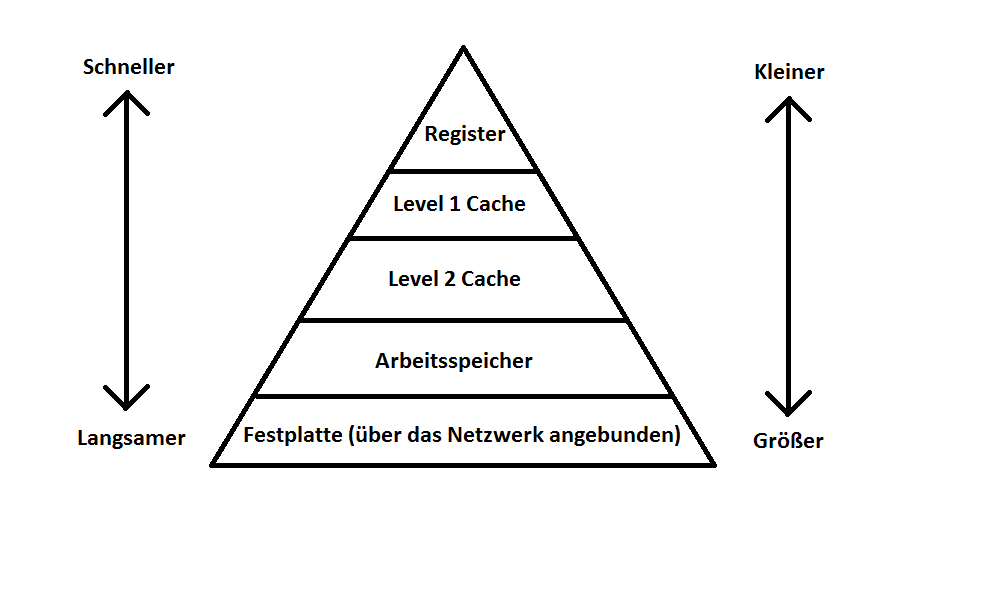
\includegraphics[height=.35\textwidth]{Bilder/hierachie.png}
	\end{center}
	\vspace*{-1cm}
	\caption{Die Speicherhierachie des E/A-Systems}
	\label{fig:mem_hierachie}
\end{figure}

Verschiedene Optimierungen und Caching-Strategien erlauben für unterschiedliches Lastverhalten eine Anpassung und somit eine effizientere Nutzung der Zwischenspeicher.
\begin{itemize}
\item \textbf{Read-Ahead:} Ein Beispiel für lesende E/A-Aufrufe ist das Einschalten der Read-Ahead-Einstellung, dadurch werden weitere Sektoren in den Cache geladen, die sich in der unmittelbaren physischen Umgebung der angefragten Datenblöcke auf dem  Speichermedium befinden. Falls ein Programm fortlaufend über einem lokal begrenzten Datenbereich arbeitet, weil dort beispielsweise direkt hintereinander Bilddateien eines Fotoalbums befinden, das gerade im Präsentationsmodus gezeigt wird, so ist der Zugriff auf ein weiteres Bild für das E/A-System nicht mehr 'überraschend'. Statt erst in dem Moment des E/A-Aufrufs des nächsten Bildes die erforderlichen Datenblöcke von der Festplatte zu lesen, befinden sich diese nun bereits in einem der vorgeschalteten Zwischenspeicher. Diese Caching-Strategie macht nur Sinn, wenn ein solches vorhersagbares (meist sequentielles) Zugriffsverhalten eines Programms stattfindet. 
Wenn aufeinanderfolgende Zugriffe in unterschiedlichen Bereichen der Festplatte Datenblöcke anfordern, wird bei dieser Strategie zusätzlicher Aufwand für das Lesen von nicht benötigten Daten betrieben (vgl. \cite{corbet2015}). 
\item \textbf{Write-Back}: Es gibt zwei Mechanismen um Daten von einen Cache auf langsameren Speicher zurückzuschreiben:
Beim Write-Through werden Schreibbefehle, die im Cache umgesetzt werden, sofort in das Speichersystem übernommen. Datenblöcke im Speichersystem und Arbeitsspeicher sind so immer identisch und daher widerspruchsfreien Zustand, sodass auch nach plötzlicher Löschung des Caches keine Informationen verloren gehen.\\
Beim Write-Back wird der geänderte Zustand von Daten zunächst nur im Cache bekannt bleibt, damit der Prozessor nicht eine lange Zeit auf die Vollendung des Schreibvorgangs auf der Festplatte warten muss. Das Ausschreiben der Änderungen im Arbeitsspeicher geschieht erst in einem günstigen Moment, wenn beispielsweise ansonsten gerade wenige E/A-Zugriffe geschehen.
\end{itemize}
Entscheidend für die optimale Wahl der Cache-Strategien und den dazu gehörenden Parametern sind jeweils die vorherrschenden Bedingungen im System, sowie dessen Benutzungsweise und die gestellten Anforderungen, die ein bestimmtes Zugriffsmuster definieren.

\section{Hochleistungsrechnen}
\label{back_hpc}
Man spricht von Hochleistungsrechnen, wenn der Rechen- oder Speicheraufwand eines Programms außerhalb dessen liegt, was ein einzelner Desktop-Computer in vertretbarer Zeit bearbeiten kann.

Notwendig wird Hochleistungsrechnen in der Forschung für die Simulation von numerischen Modellen aus verschiedensten Bereichen, beispielsweise für Mehrkörpersimulationen in der Astronomie, für Strömungssimulationen oder zur Berechnung von Klimaprognosen.

Die im Hochleistungsrechnen verwendeten Computer werden als Supercomputer bezeichnet, hierbei handelt es sich heutzutage üblicherweise um Rechnerverbünde (engl. Cluster) in denen eine große Anzahl Prozessoren und Speichermedien verbunden werden.
Die übliche Struktur sieht dabei so aus, dass eine Vielzahl Rechnerknoten durch ein gemeinsames Netzwerk zusammengeschaltet werden. Bei einem Rechnerknoten handelt es sich um ein Mehrprozessorsystem mit gemeinsamen Speicher. Jeder Prozessor im Knoten hat einen eigenen Cache mit dem er arbeiten kann, zudem gibt es einen Speicher, auf den alle Prozessoren gemeinsam zugreifen. 
Der Verbund aus Rechnerknoten, der den Hochleistungsrechner bildet, verfügt wiederum über einen gemeinsamen Speicher. Dabei handelt es sich um das Speichersystem des Hochleistungsrechners, das über das Netzwerk mit den einzelnen Rechnerknoten verbunden ist.
Eine Darstellung einer typischen Struktur eines Hochleistungsrechners ist in Abbildung \ref{fig:rechnerknoten} zu sehen.
\begin{figure}[h]
	\begin{center}
		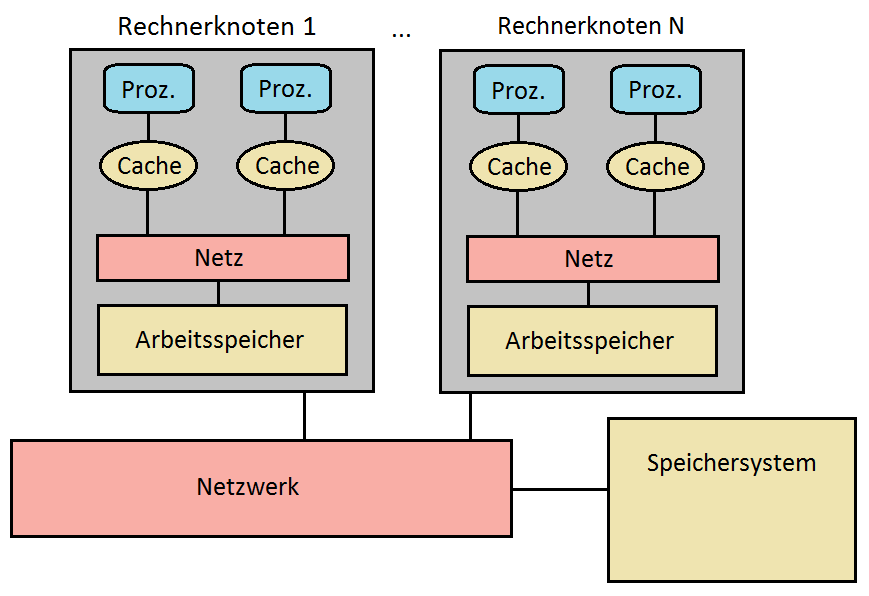
\includegraphics[width=.43\textwidth]{Bilder/rechnerknoten.png}
	\end{center}
	\caption{Typische Struktur eines Hochleistungsrechners}
	\label{fig:rechnerknoten}
\end{figure}

Wichtige Themen im Hochleistungsrechnen sind die effiziente Ausnutzung der zur Verfügung stehenden Leistung, das Erkennen und Beheben von Fehlern des parallelisierten Programmcodes, die Bereitstellung der Rechen- und Speicherkapazitäten, sowie die Energieeffizienz von Hard- und Software.
Um einen Supercomputer gut ausnutzen zu können ist bei vielen Anwendungen eine leistungsfähige Ein-/Ausgabe von großer Wichtigkeit. Bedingt ist dies dadurch, dass die Menge der anfallenden Daten wesentlich stärker ansteigt, als die Geschwindigkeit der Verbindungen zwischen den verschiedenen Speichermedien und -orten.

Die in Abschnitt \ref{back_E/A} beschriebene Ein-/Ausgabe erweitert sich im Rechnerverbund zur parallelen E/A, dies bedeutet einerseits, dass eine Datei von mehreren Prozessen zeitgleich gelesen und bearbeitet werden kann, und andererseits, dass eine Datei über mehrere Festplatten und Netzwerk-Server verteilt sein kann. Diese Parallelität hat einen wesentlichen Einfluss auf die E/A-Leistungsvorhersage, denn statt nur den Aufwand der Arbeitsschritte auf einer einzelnen Festplatte abzuschätzen, müssen hier die verstrickten Zusammenhänge zwischen Netzwerken von Festplatten und Rechnern, den jeweiligen Auslastungen der Komponenten, sowie Priorisierungen bestimmter Aufgaben und Instanzen durch die Speicherverwaltung berücksichtigt werden.

Die Erfassung aller dieser Informationen wäre sehr aufwendig, sodass dies zur Zeit nicht möglich ist. Eine Vorhersage von E/A-Leistung eines parallelen Dateisystems ist daher sehr nicht trivial.

\section{Maschinelles Lernen}
\label{back_ML}
Maschinelles Lernen gehört zu den Themengebieten künstliche Intelligenz und automatisierte Wissensgenerierung. Verfahren dieser Disziplin versuchen durch intelligentes Lernen von Mustern Vorhersagen und Entscheidungen zu treffen.
Als intelligent wird ein maschinelles Verfahren bezeichnet, dass vorgegebene Informationen nicht auswendig lernt und wiedergibt, sondern von diesen Informationen abstrahiert.
Durch eine globale Sichtweise auf die Daten können Gesetzmäßigkeiten zwischen den Trainingsdaten erkannt werden.
Als \textbf{Trainingsdaten} werden die Informationen bezeichnet, die dem Algorithmus beim Aufbau (Training) des Modells bekannt sind.
Ein \textbf{Testdatensatz} dagegen ist eine Menge von ungesehenen Daten mit denen die Ergebnisse des maschinellen Lernens verglichen werden können.
Ein \textbf{Attribut} ist eine messbare Größe der Objekte, die untersucht werden. Dies könnte beispielsweise bei einem Datensatz über Blumen die Farbe der Blütenblätter sein.
Ein Datenpunkt (oder auch eine Instanz) beschreibt ein spezifisches Objekt (z.B. ein bestimmtes Exemplar der Blume), dazu enthält er einen an der Instanz gemessenen Wert zu jedem Attribut.

Typische Aufgaben des maschinellen Lernens sind die Clusteranalyse und die Regressionsanalyse.

\begin{itemize}
\item Bei der \textbf{Clusteranalyse} muss von den eigentlichen Objekt-Attributen einzelner Datenpunkte abstrahiert werden, sodass Zusammenhänge zwischen den Objekten erkannt werden können. Dann können Klassengrenzen definiert werden, die jeder Klasse einen Bereich des Attribut-Raumes zuordnet.
Als \textbf{Klassierung} bezeichnet man die Zuordnung eines Objekts mit spezifischen Attributen in die definierten Klassen. Dazu müssen die Attribut-Werte des Objekts nur mit den Klassengrenzen vergleichen werden.
\item \textbf{Regressionsanalyse} (oft auch nur Regression) ist ein Verfahren zur Bestimmung der Zusammenhänge von einer spezifischen Zielvariablen zu den übrigen Objekt-Attributen. Wenn in einem Datensatz die Einträge zur Zielvariablen fehlen, können die berechneten Relationen zur Prognose der unbekannten Werte mit Hilfe der bekannten Attribute genutzt werden. Die Zielvariable wird so über die Abhängigkeit zu anderen Variablen durch ein Verfahren des maschinellen Lernens modelliert. Das erhaltene Modell aus dem Verfahren wird auch als Prädiktor bezeichnet. 	
\end{itemize}

Ein Verfahren bzw. Algorithmus des maschinellen Lernens erstellt für die Cluster- bzw. Regressionsanalyse ein Modell, welches einerseits Aussagen über die zur Verfügung stehenden Daten trifft und darüber hinaus, abgeleitet aus den inneren Abhängigkeiten der Daten, Aussagen über bislang unbekannte Objekte treffen kann.
Bei der Clusteranalyse wird eine qualitative Aussage über neue Datenpunkte anhand der Einordnung in Gruppen getroffen.
Beim Regressionsmodell wird dagegen eine quantitative Aussage über die Zusammenhänge zwischen den Attributen der Daten getroffen. 
Clusteranalyse und Regression können weitergehend über ihr Lernverhalten unterschieden werden.
Während bei der Regression überwachtes Lernen stattfindet, wird bei der Clusteranalyse unüberwacht gelernt. Der Unterschied der beiden Varianten befindet sich in den Informationen die im Trainingsdatensatz enthalten sind.
\begin{itemize}
\item Beim unüberwachten Lernen wird kein bestimmtes Ergebnis erwartet, stattdessen muss der Algorithmus versuchen den Informationen inhärente Abhängigkeiten und Zusammenhänge zu erkennen.
Wenn die Klassenzuordnungen bereits in den Trainingsdaten bekannt wären, hätte die Clusteranalyse nicht viel zu tun. 
Der Clusteranalyse steht daher während des Lernprozesses auch keine Rückmeldung über die Güte der gemachten Klassen zur Verfügung.
\item Die \textbf{Instanzen} der Trainingsdaten beim überwachten Lernen enthalten auch die gesuchten Werte der Zielvariablen, deren Werte der Algorithmus nach dem Lernvorgang auf dem Testdatensatz vorhersagen soll.
Für die Regressionsanalyse sind diese Informationen essentiell, da für die Modellierung die Zusammenhänge der Werte der Zielvariablen mit den restlichen Variablen untersucht werden muss.
Die Information über die idealen Ausgabewerte der Zielvariablen werden während des Lernvorgangs genutzt um die Parameter des Prädiktors so anzupassen, dass er die vorgegebenen Werte möglichst gut approximiert. Wichtig ist dabei, dass der Prädiktor nicht zu sehr auf die Trainingsdaten zugeschnitten wird, sondern die abstrakteren Relationen erkennt, sodass auch auf den ungesehenen Testdaten gut vorhersagen gemacht werden können.
\end{itemize}

Die bei der Clusteranalyse erstellten Gruppierungen werden üblicherweise nicht bewertet, da die Qualität einer Sortierung nur im Kontext des gewünschten Nutzens der Klassen beurteilt werden kann.
Zunächst einmal ist jede eindeutige Klassierung legitim.

Der Prädiktor der Regressionsanalyse kann dagegen konkret bewertet werden. Dazu wird der Testdatensatz benötigt. Die zu bestimmenden Werte der Zielvariablen sind in den Testdaten bereits vorgegeben.
Diese Information wird bei der Durchführung des Tests vorenthalten. Durch den Vergleich zwischen tatsächlicher und vorhergesagter Lösung können Rückschlüsse auf die Qualität der Vorhersagen gezogen werden können. Dazu werden Metriken zur Bestimmung der Güte der Modellierung benötigt.
Zur Anwendung einer Regressionsanalyse müssen also zunächst Kriterien bzw. Leistungsmetriken eingeführt werden, anhand derer die Qualität der Vorhersagen und Entscheidungen gemessen werden können. Einerseits zum Vergleich der Vorhersagen auf den Testdatensatz zwischen verschiedenen Ansätzen, andererseits aber auch schon für den Lernprozess des Algorithmus selbst, damit dieser sozusagen aus seinen Fehlern und Erfolgen lernen kann. Eine einfache Metrik wäre beispielsweise die mittlere Modellabweichung der Vorhersagen gegenüber den \textit{Lösungswerten}.
\medskip

Oft ist es notwendig die zur Verfügung stehenden Daten aufzubereiten, bevor ein maschineller Lernalgorithmus effizient und korrekt Informationen aus diesen ableiten kann.
Nach Alpaydin können fehlerhafte Daten ein Problem sein, die durch zufällige Messfehler oder eine systematisch inkorrekte Messung entstehen können (vgl. \cite{Alpaydin:2010:IML:1734076} S. 13-15). Zudem schreibt er, dass Teile der Daten überflüssig sein können, da sie redundant sind oder keine relevanten Informationen enthalten. Problematisch sind auch Datenpunkte mit gleichen Eingabewerten, aber unterschiedlichen Werten zur Zielvariablen (vgl. \cite{Alpaydin:2010:IML:1734076} S. 14).
Mit all diesen Problemen muss, unter Beachtung der Eigenschaften des vorliegenden Datensatzes, bei der Aufbereitung der Daten sinnvoll umgegangen werden. So können beispielsweise Ausreißer bei den Daten aussortiert werden, da diese eventuell durch eine Fehlmessung entstanden sind. Widersprüchliche Datenpunkte können zusammengefasst werden, indem sie zusammen einen neuen Datenpunkt mit eindeutigen Ausgabewerten bilden (dies könnten die Mittelwerte sein).

\subsubsection{Clusteranalyse}
Kantardzic beschreibt die Clusteranalyse folgendermaßen: \glqq Cluster analysis is the formal study of methods and algorithms for natural grouping, or clustering, of objects according to measured or perceived intrinsic characteristics or similarities.\grqq{} \cite{kantardzic2011data} (S. 250). Ein einfaches und anschauliches Beispiel sind Punkte im zweidimensionalen Raum, die hinsichtlich ihrer Position gruppiert werden. Die beiden Dimensionen können hierbei als unabhängige Attribute der Objekte verstanden werden (vgl. Abbildung \ref{fig:clustering_beispiel}).

\begin{figure} [h]
	\subfloat{
		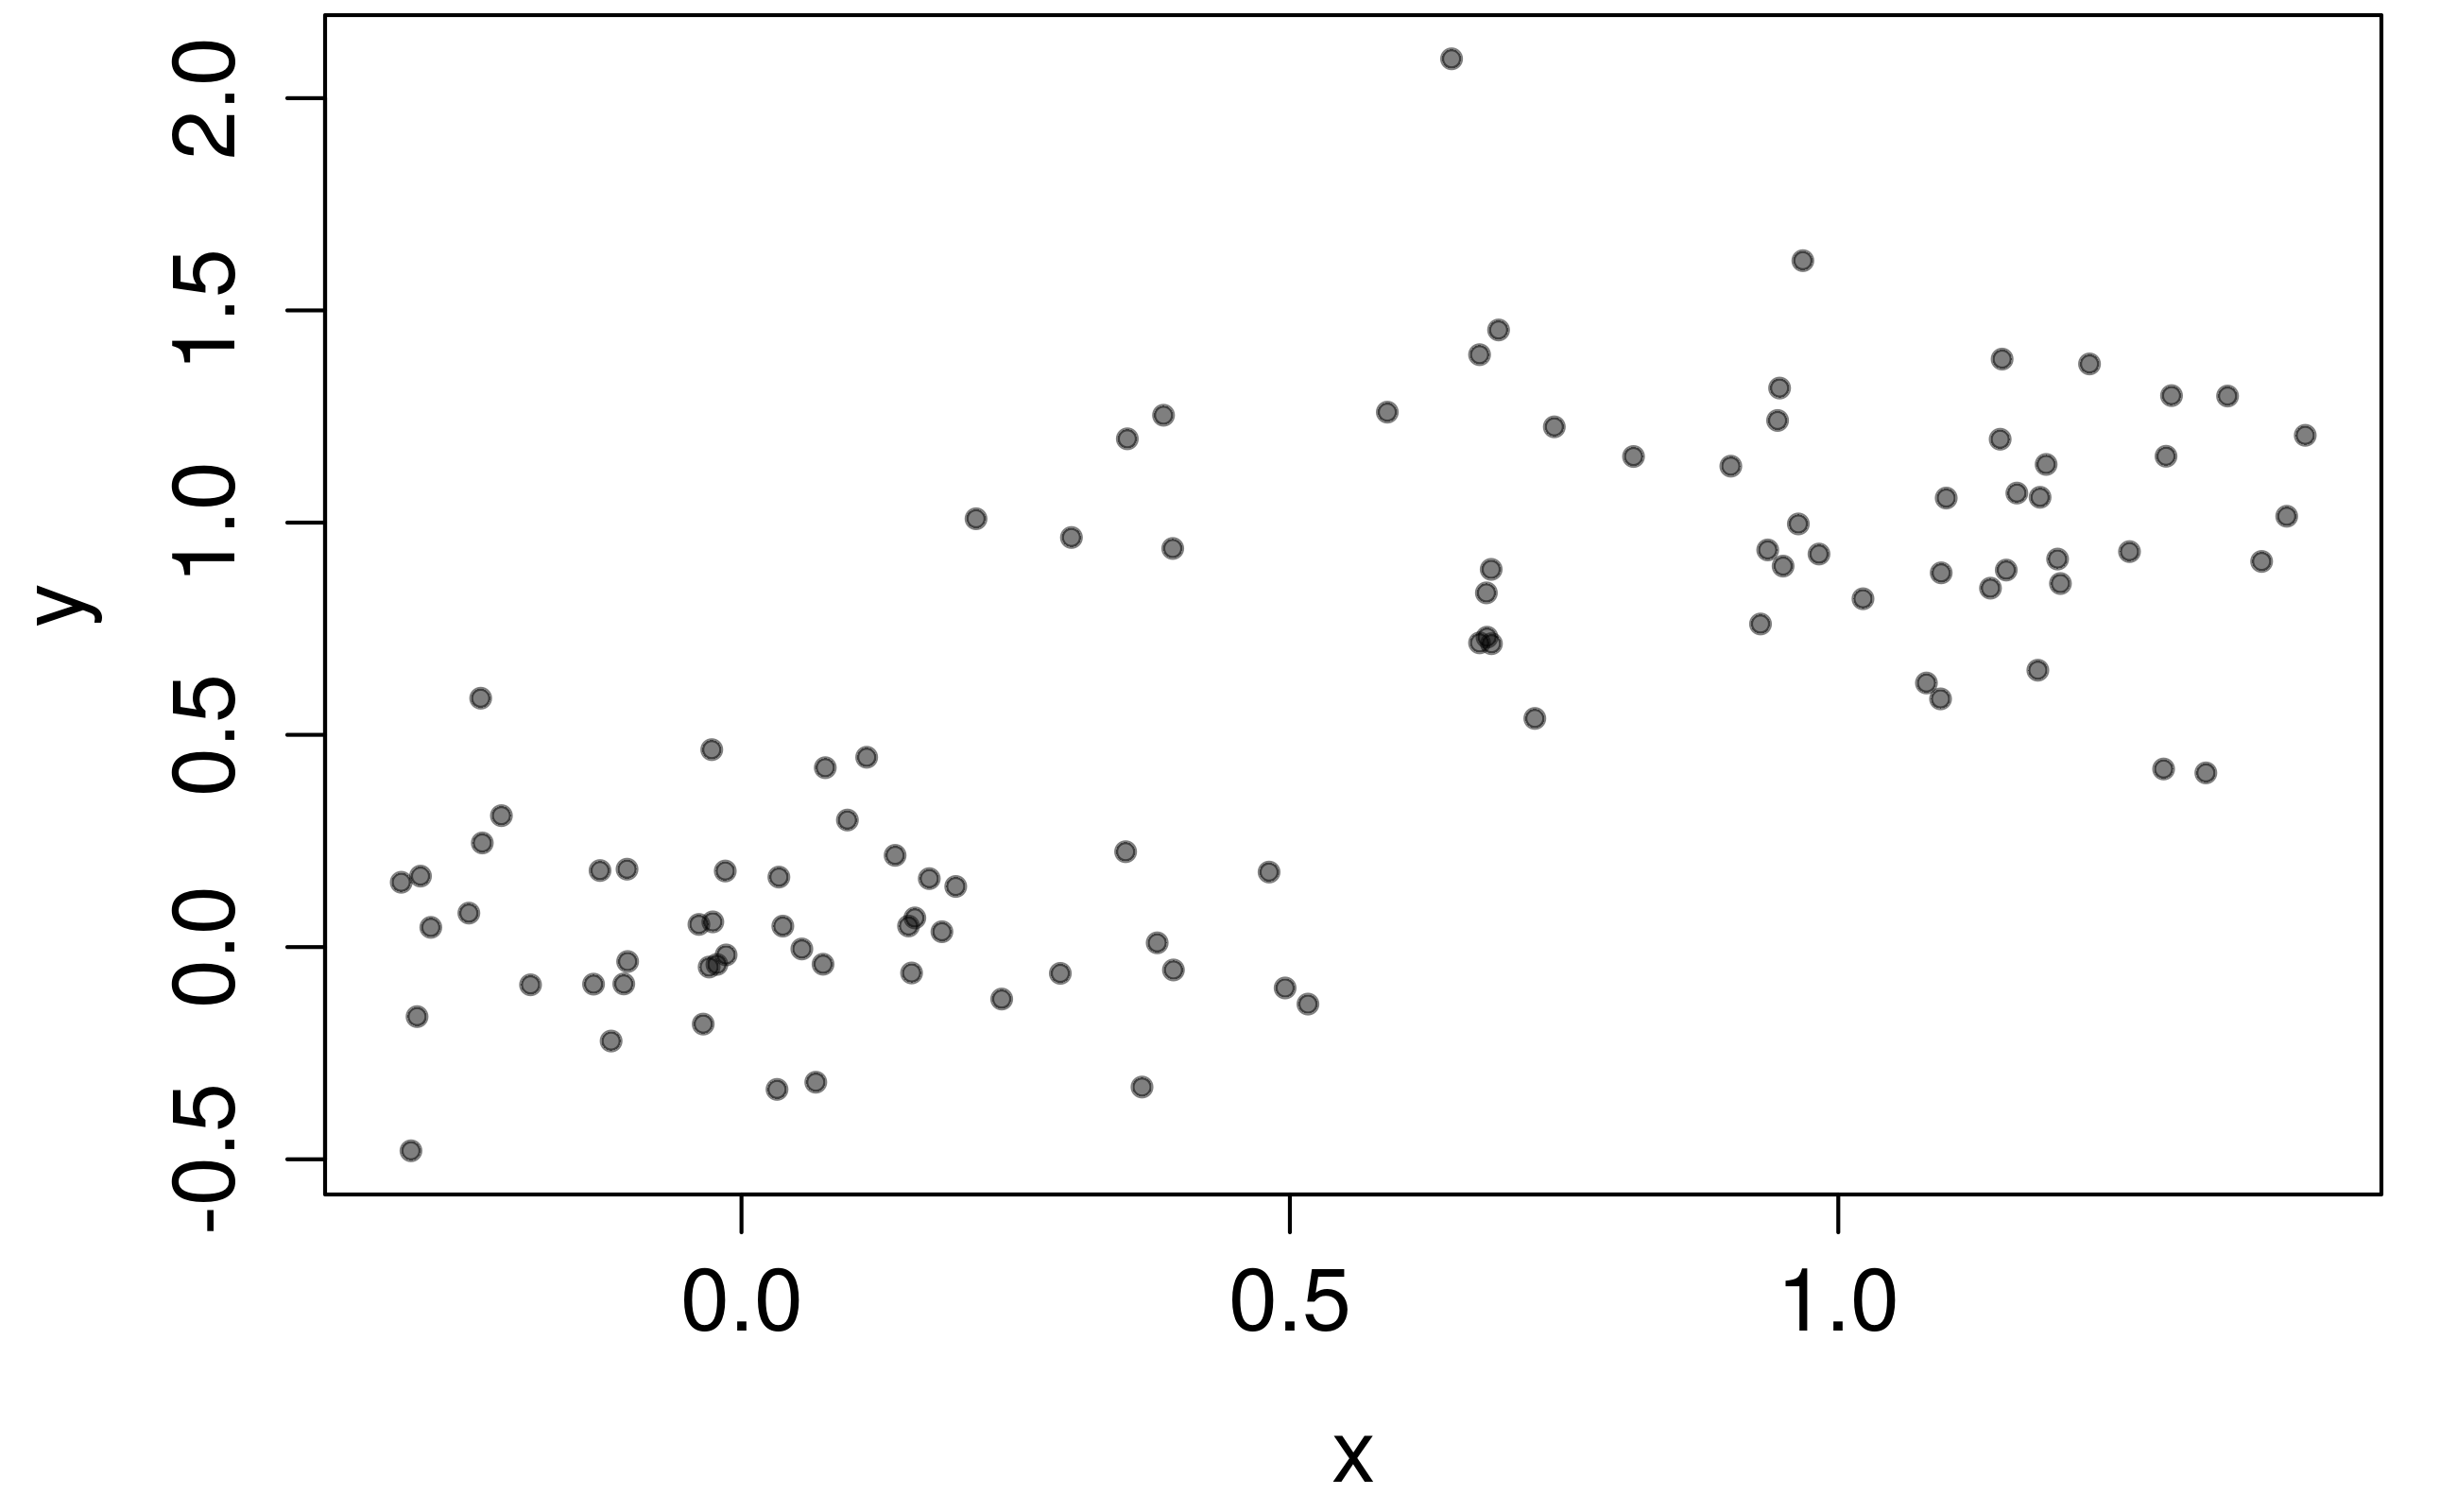
\includegraphics[width=.5\textwidth]{Bilder/test_clustering_points.png}
	}
	\hfill
	\subfloat{
		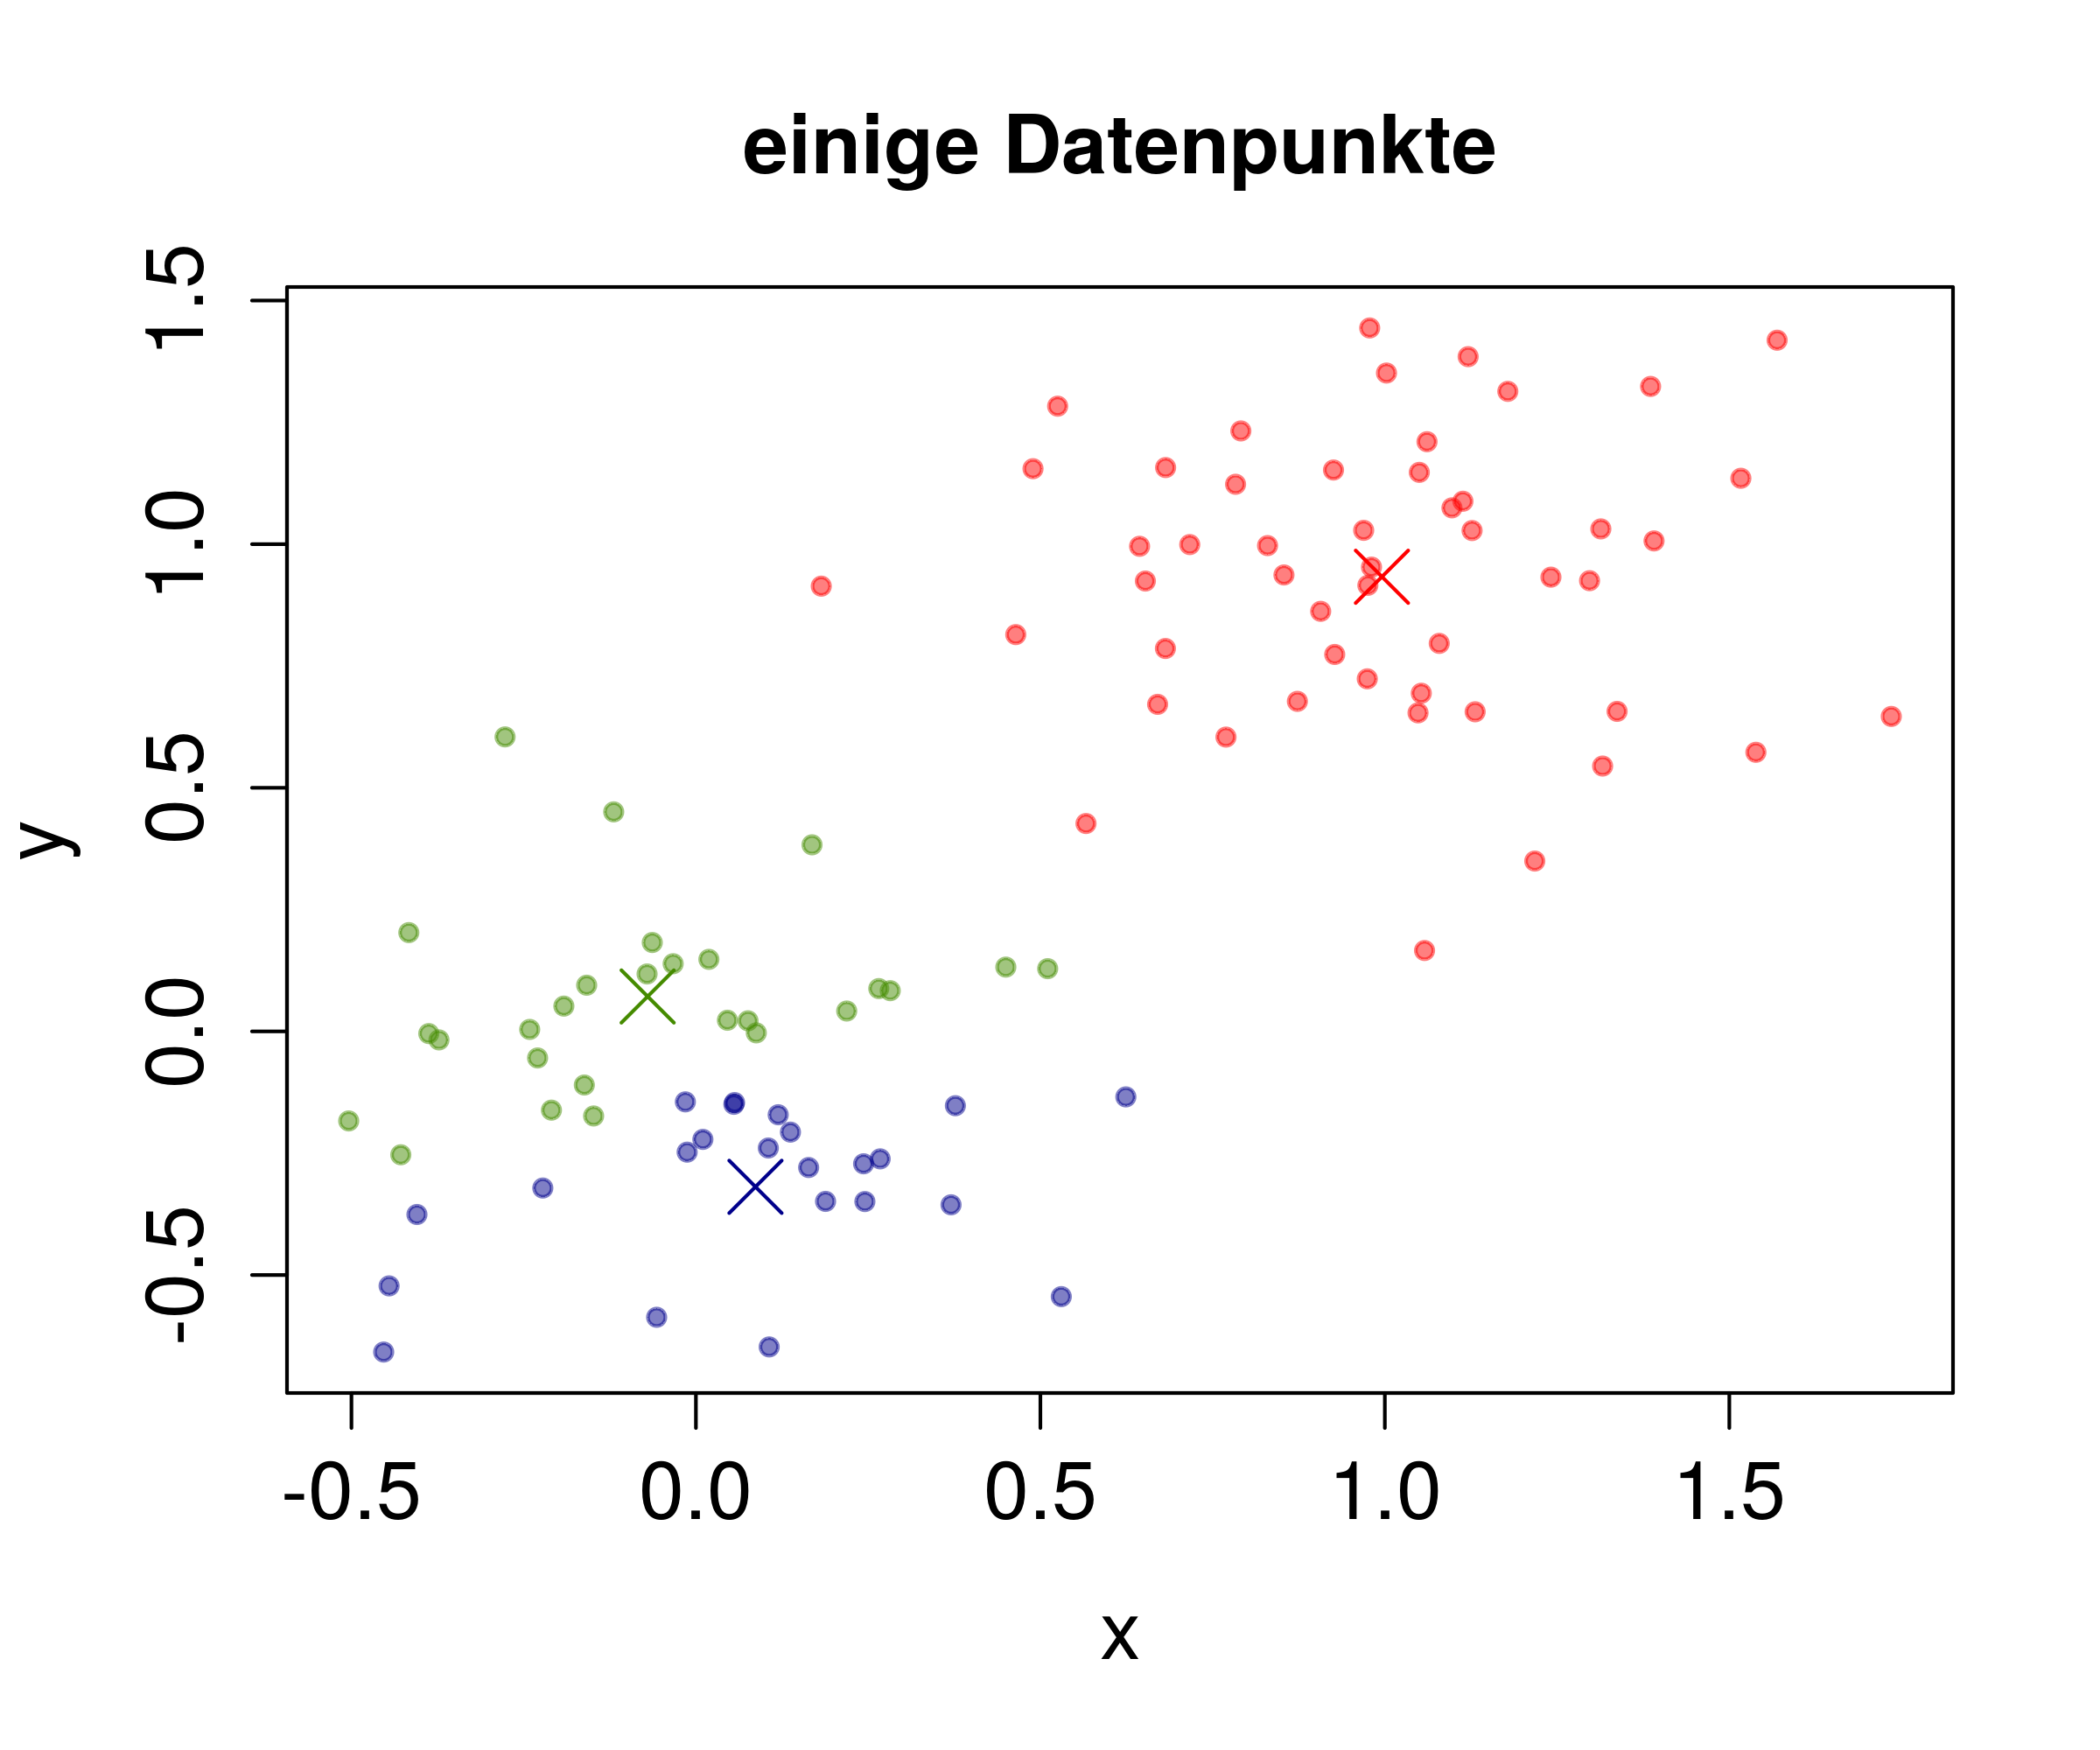
\includegraphics[width=.5\textwidth]{Bilder/test_clustering.png}
	}	
	\caption{Datenpunkte mit je einem Wert für x und y-Dimension. Rechts farbliche Markierung für die Zugehörigkeit zu den drei vom k-Means-Algorithmus bestimmten Clustern. Ein Kreuz markiert den Mittelpunkt jedes Clusters (Mittelwert aller zugehörigen Punkte)}
	\label{fig:clustering_beispiel}
\end{figure} 

Ein einfacher Clustering-Algorithmus ist der k-Means-Algorithmus. Bei diesem muss vom Benutzer zunächst die Anzahl Cluster $k$ festgelegt werden. 
Der Algorithmus geht dann wie folgt vor:\\
Die $k$ Mittelwerte der Cluster werden mit zufälligen Werten initialisiert. Dann wird jeder Datenpunkt dem Cluster zugeordnet, dessen Mittelwert seinem am nächsten ist. Danach werden die Mittelwerte der Cluster anhand der Ihnen zugeordneten Punkte berechnet und gesetzt. Das Neuzuordnen der Punkte und Berechnen der Mittelwerte wird nun solange wiederholt, bis sich keine Änderung der Zuordnung mehr ergibt. Als Endergebnis des k-Means-Algorithmus erhält man eine Gruppierung der Datenpunkte in Mengen mit möglichst niedriger Varianz innerhalb eines Clusters und möglichst großer Varianz von Punkten in verschiedenen Clustern.

\section{Künstliche Neuronale Netze}
\label{back_nn}
Bei künstlichen neuronalen Netzen, im Folgenden meist nur neuronale Netze genannt, handelt es sich um eine Methode aus dem Bereich des maschinellen Lernens zum Approximieren einer unbekannten Funktion. Die Methode ist inspiriert von biologischen neuronalen Netzen, wie sie im Gehirn vorkommen. 
Sie verwenden einen statistischen Ansatz, ihre Lösung für das Problem wird zunächst zufällig im Lösungsraum angelegt und dann mit Hilfe eines Gradientenverfahrens optimiert.
Rojas vergleicht neuronale Netze mit einer Black Box, also einem System mit beobachtbarer Ein- und Ausgabe, aber unbekannter innerer Verarbeitung der Informationen \cite{Rojas:1996:NNS:235222}. 
Zur Verwendung eines neuronalen Netzes gibt man dem Netz eine Menge von Eingabevektoren $E \in \mathbb{R}^n$ mit jeweils zugehörigem Ausgabevektor $A \in \mathbb{R}^m$ vor und dieses versucht eine passende Funktion $F: \mathbb{R}^n \rightarrow \mathbb{R}^m$ zu finden. Dementsprechend handelt es sich hierbei um überwachtes Lernen, da eine gewünschte ideale Ausgabe vorgegeben wird.

\begin{figure}[h]
	\begin{center}
		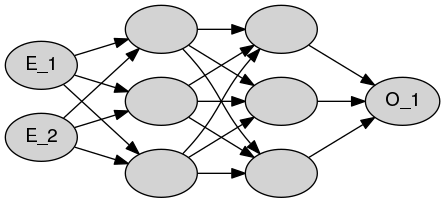
\includegraphics[height=.20\textwidth]{Dot/netz.png}
	\end{center}
	\caption{feedforward-Netz mit $n=2$, $m=1$ und 2 verborgenen Schichten}
	\label{fig:Schichten}
\end{figure}

Die häufigste verwendete Art neuronaler Netze sind feedforward-Netze. Sie bestehen aus einer Eingabeschicht, einer beliebigen Anzahl verborgener Schichten und einer Ausgabeschicht (siehe Abbildung \ref{fig:Schichten}), wobei die Verbindungen aus jeder Schicht jeweils nur in die darauf folgende Schicht gehen (vgl. Abbildung \ref{fig:Neuron}).
Die Eingabeschicht besteht, der vorherigen Definition entsprechend, aus $n$ Stellen, an denen die Werte eines Eingabevektors stehen. Jeder Eingabewert wird dann an jedes Neuron in der ersten verborgenen Schicht weitergegeben und dort verrechnet, die Ergebnisse der Neuronen der verborgenen Schicht werden dann an die nächste Schicht gegeben und so weiter.
Die Ergebnisse der Ausgabeschicht bilden den Ausgabevektor mit Länge $m$.\\
Rekurrente Netze haben die gleiche Struktur, doch es können auch Verbindungen zu zurückliegenden Schichten vorkommen, dadurch ist die Berechnung zu einem Eingabevektor nicht mehr deterministisch bestimmt, sodass entsprechende Regeln festgelegt werden müssen.

\begin{figure}[h]
	\begin{center}
		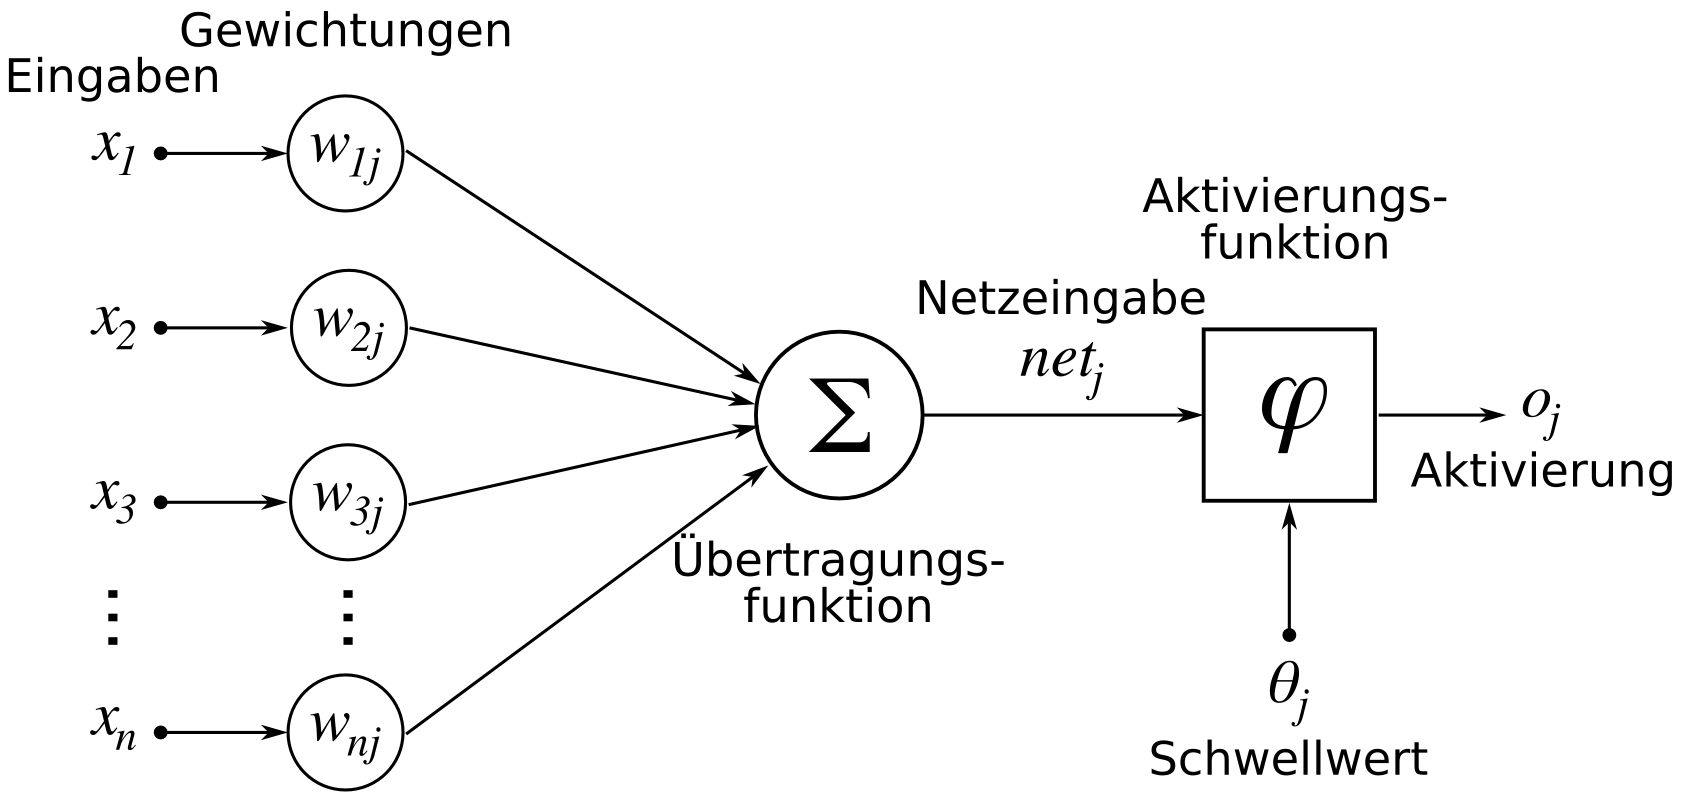
\includegraphics[totalheight=0.2\textheight]{Bilder/ArtificialNeuronModel_deutsch.png}
	\end{center}
	\caption{Schema eines künstlichen Neurons. Quelle: Chrislb, \url{https://de.wikipedia.org/wiki/Datei:ArtificialNeuronModel_deutsch.png}} %
	\label{fig:Neuron}
\end{figure}

\subsubsection{Berechnungsregeln}
Jedes Neuron rechnet die eingehenden Eingabewerte mit einer zur Übertragungskante zugehörigen Gewichtung mit einer Übertragungsfunktion zusammen; die Anzahl der Eingaben ist hierbei unbegrenzt (vgl. \glqq unlimited fan-in property\grqq{} \cite{Rojas:1996:NNS:235222}). Die Übertragungsfunktion kann hierbei schlicht die Summe aller gewichteten Eingaben sein. Der errechnete Wert wird als Netzeingabe an die Aktivierungsfunktion gegeben. 
Die Aktivierungsfunktion berechnet eventuell mit oder ohne einem Schwellwert die Aktivierung des Neurons, welche dann an alle verbundenen Neuronen der nächsten Schicht weitergegeben wird.
Die Aktivierungsfunktion kann beispielsweise eine simple Stufenfunktion sein, die allen Netzeingaben kleiner des Schwellwerts eine Null und allen Eingaben größer gleich des Schwellwerts eine Eins zuweist.

Ein Neuron mit der gewichteten Summe aller Eingaben als Übertragungsfunktion und einer Stufenfunktion mit Schwellwert als Aktivierungsfunktion wird von Rojas \textit{Perzeptron} bezeichnet (vgl. \cite{Rojas:1996:NNS:235222} S. 60).
\medskip

Ein feedforward-Netzwerk aus Perzeptrons, in dem jedes Neuron mit allen Neuronen der folgenden Schicht verbunden ist, wird als \textit{multilayer perceptron} (kurz MLP) bezeichnet.

\subsubsection{Trainieren von neuronalen Netzen}
Ein neuronales Netz lernt die Abbildung zwischen den vorgegebenen Paaren von Eingabe- und Ausgabedaten durch Anpassung der Gewichte an den Kanten, nachdem es mit zufälligen Kantengewichten initialisiert wurde.
Diese Anpassung geschieht beim MLP durch Fehlerrückführung (engl. backpropagation). Dabei wird der mittlere quadratische Fehler der berechneten Ausgabe gegenüber der vorgegebenen idealen Ausgabe ermittelt und daraufhin unter Rücksichtnahme auf eine Lernrate mit Hilfe des Gradientenverfahren minimiert (vgl. \cite{Rojas:1996:NNS:235222} S.151 ff.).

\subsubsection{Berechenbarkeitstheorie neuronaler Netze}
Vor der Anwendung von künstlichen neuronalen Netzen für ein Problem stellt sich die Frage, ob diese für das Problem geeignet sind. Dazu gibt es einige interessante mathematische Beweise.
Ein einzelnes Perzeptron kann alle linear separierbaren logischen Funktionen exakt approximieren (vgl. \
{Rojas:1996:NNS:235222} S. 62-63), wobei lineare Separierbarkeit nach Rojas definiert ist als:

Zwei Punktmengen A und B in einem n-dimensionalen Raum sind linear separierbar, wenn $n + 1$ reelle Zahlen $w_1,...,w_{n+1}$ existieren, sodass für jeden Punkt $(x_1,x_2,...,x_n) \in A$ die Ungleichung $\sum_{i=1}^{n} w_ix_i \ge w_{n+1}$ gilt und für jeden Punkt $(x_1,x_2,...,x_n) \in B$ $\sum_{i=1}^{n} w_ix_i < w_{n+1}$\medskip

Beispiele für (nicht) linear separierbare Mengen sind in Abbildung \ref{fig:separierbarkeit} dargestellt.

\begin{figure}
	\centering
	\subfloat[Zwei voneinander nicht linear separierbare Relationen in $ \mathbb{R}^2$.]{
		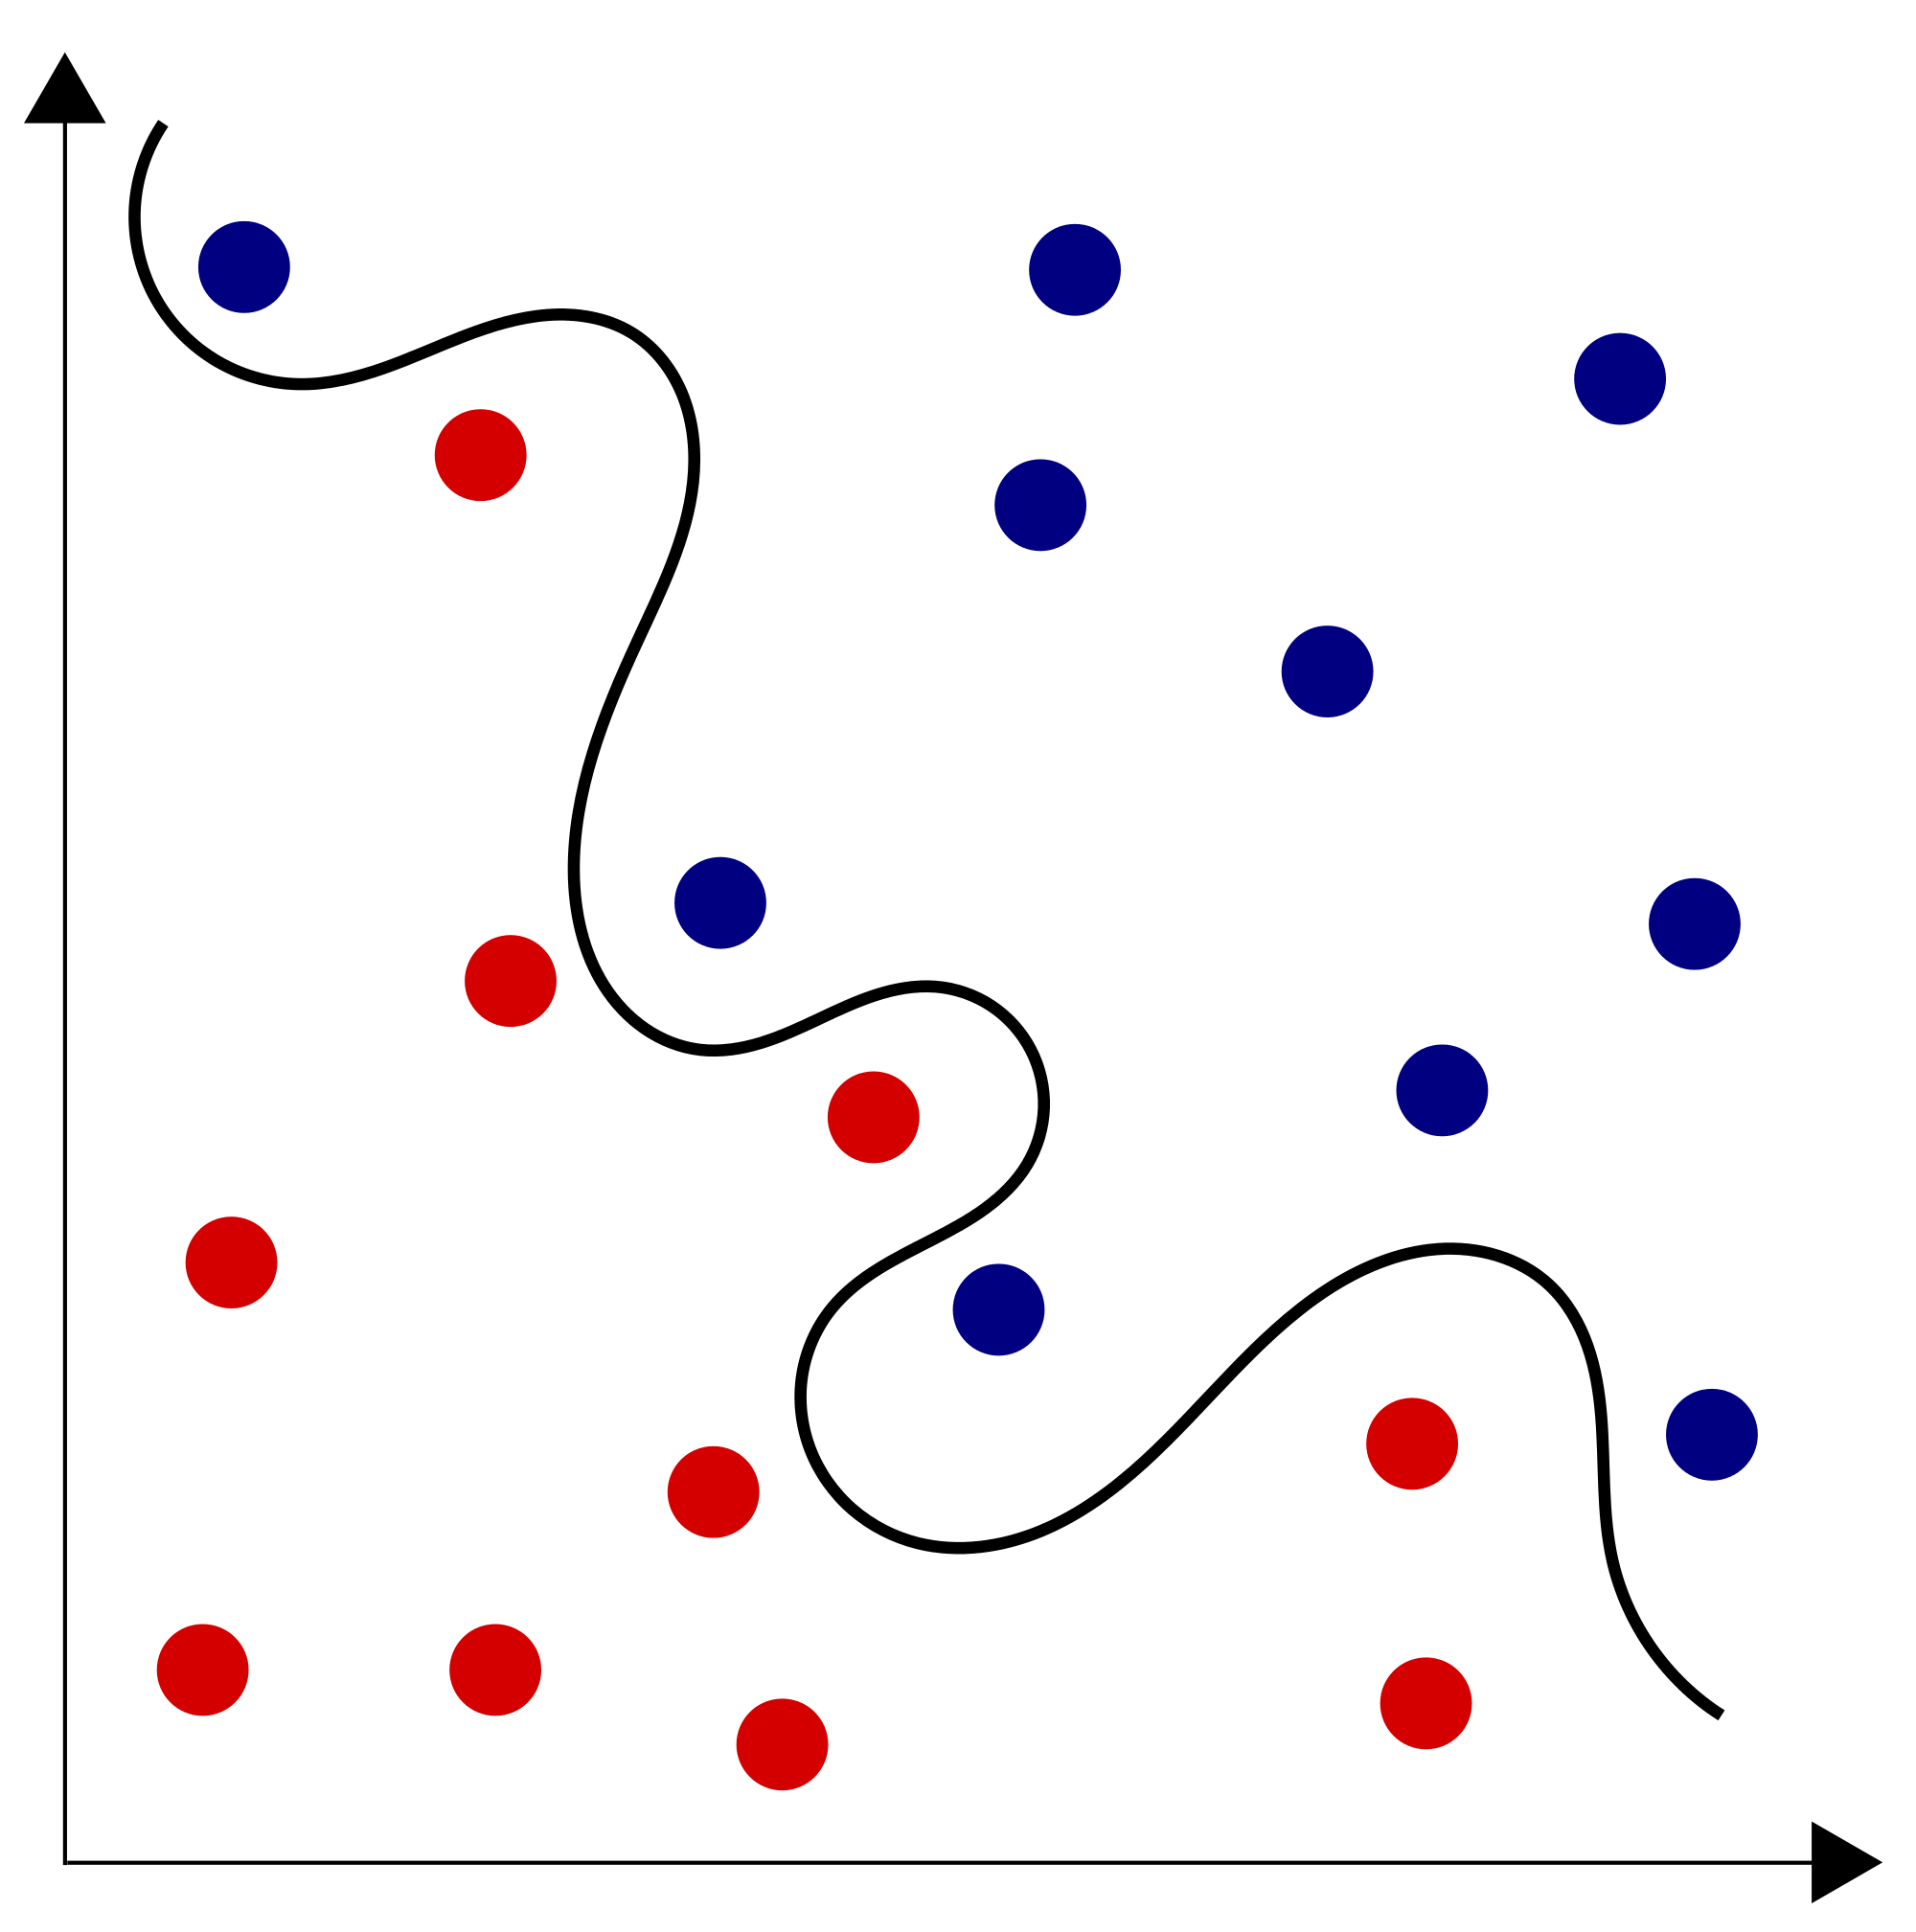
\includegraphics[width=.3\textwidth]{Bilder/2000px-Separability_NO.png}
	}
	\hfill
	\subfloat[Zwei voneinander linear separierbare Relationen in $\mathbb{R}^2$.]{
		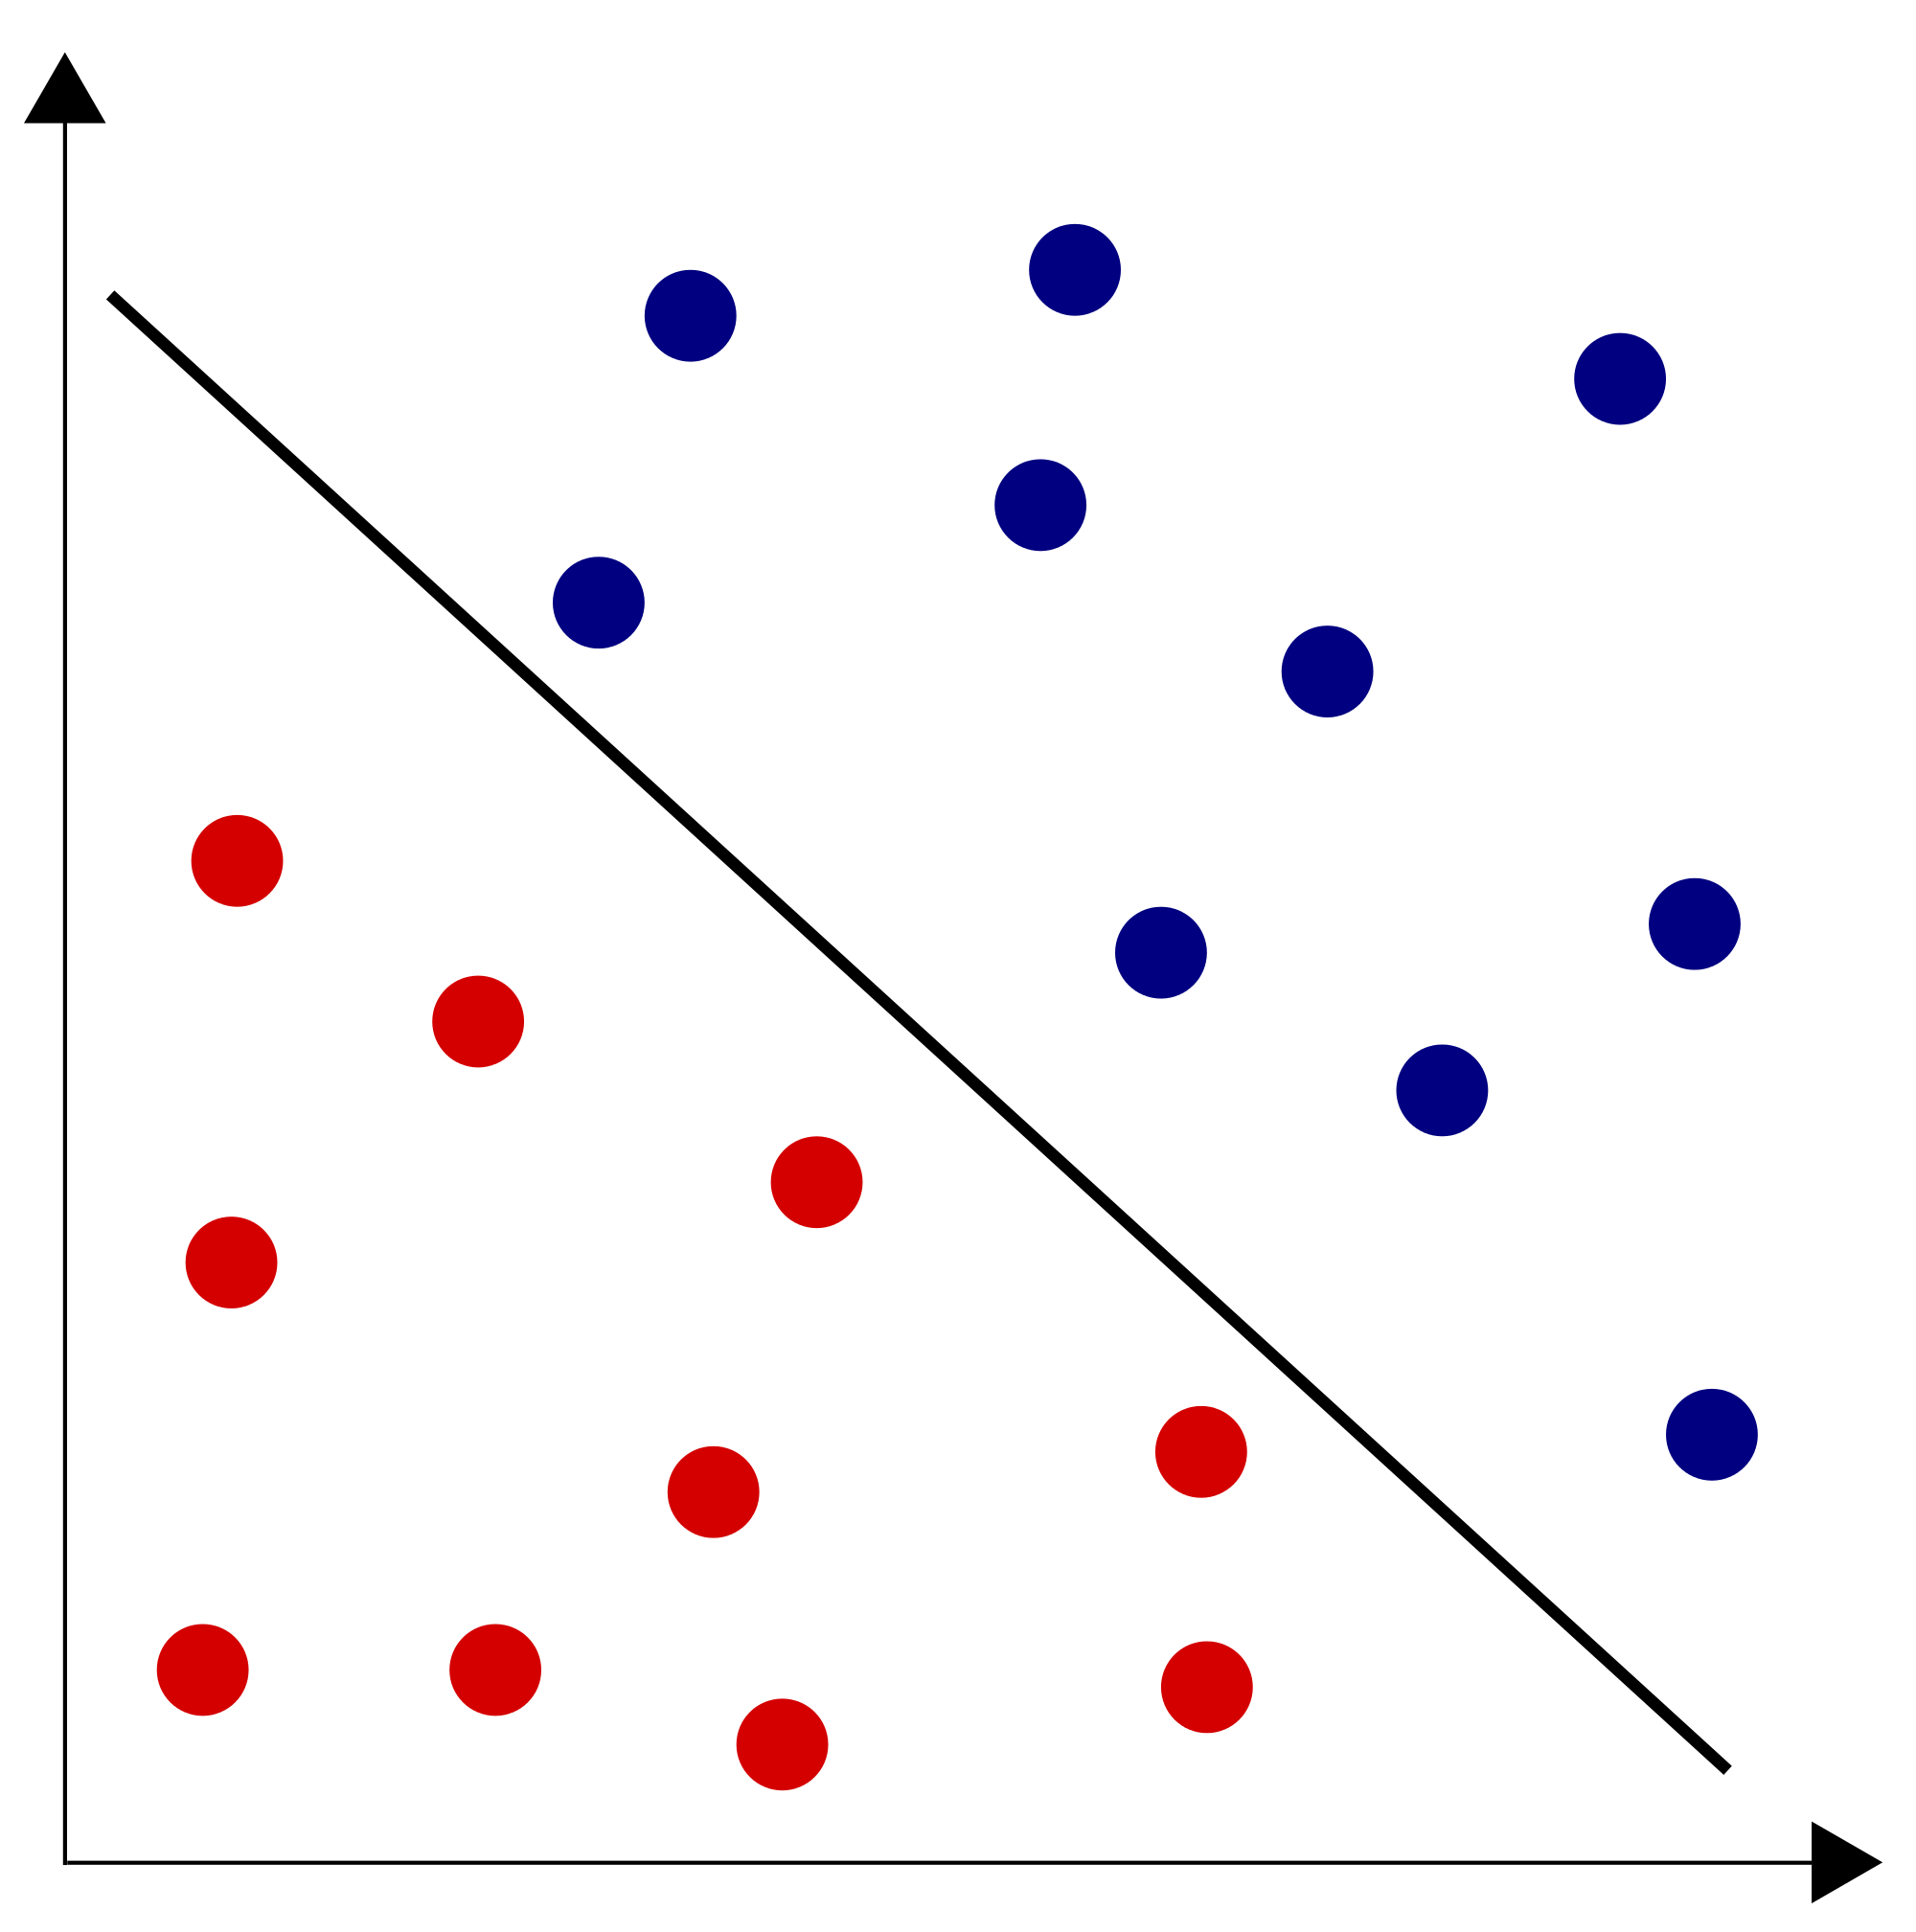
\includegraphics[width=.3\textwidth]{Bilder/2000px-Separability_YES.png}
	}		
	\caption{Lineare Separierbarkeit, Quelle: Mekeor, \url{https://de.wikipedia.org/wiki/Datei:Separability_YES.svg} und \url{https://de.wikipedia.org/wiki/Datei:Separability_NO.svg}}
	%
	\label{fig:separierbarkeit}
\end{figure} 

Diese Beschränkung gilt allerdings nicht für ein Netzwerk von Neuronen. Bereits ein zweilagiges Netzwerk aus noch simpleren McCulloch-Pitts-Zellen kann jede beliebige logische Funktion berechnen (vgl. \cite{Rojas:1996:NNS:235222} S. 37).
Für MLPs hat Cybenko \cite{cybenko:mcss} bewiesen, dass sie beliebige kontinuierliche Funktionen auf einer kompakten Teilmenge des euklidischen Raums $\mathbb{R}^n$ approximieren können. Der entsprechende Satz hierzu ist das \textit{universal approximation theorem}.

\bigskip
\paragraph{Zusammenfassung:}
\textit{ 
	Das Kapitel hat einen kurzen Abriss der für diese Thesis relevanten Themen geliefert. Es wurde festgestellt, dass die Vorhersage von E/A-Laufzeiten im Hochleistungsrechnen eine komplexe Aufgabe ist. Zusätzlich zu dem ohnehin aufwendigen E/A-System eines normalen Rechners müssen die Komplikationen durch die Vernetzung des Hochleistungsrechners in Betracht gezogen werden.\\
	Das Problem der E/A-Leistungsvorhersage kann mit Hilfe maschinellen Lernens gelöst werden. Die Aufgabe entspricht dabei einer Regressionsanalyse. Für das überwachte Lernen müssen Trainingsdaten in der Form gemessener Zugriffszeiten von E/A-Aufrufen bereit stehen. Dabei werden die Abhängigkeiten zwischen Aufrufparametern und Zugriffszeit ausgenutzt um die unbekannten Laufzeiten unbekannter Zugriffe vorherzusagen.
	Solange die E/A-Leistung durch eine kontinuierliche Funktion beschrieben werden kann und alle dafür benötigten Informationen zur Verfügung stehen, kann ein künstliches neuronales Netz das Problem lösen.\\
	Im folgenden Kapitel werden verwandte Arbeiten vorgestellt, in denen das Problem der Leistungsvorhersage bereits behandelt wurde.
}

\chapter{Verwandte Arbeiten}
\label{verwandte_arbeiten}
\textit{%
	In diesem Kapitel werden wissenschaftliche Veröffentlichungen vorgestellt, die dieser Arbeit gegenüber relevante Themen behandeln. Es werden drei Teilgebiete des Problems der Leistungsvorhersage von E/A-Aufrufen im Hochleistungsrechnen behandelt.\\
	Als Erstes gehe ich in Abschnitt \ref{rel_ea-vorhersage} auf einige Arbeiten ein, die allgemeine E/A-Leistungsvorhersage behandeln. Dabei führe ich zunächst zwei Begriffe für Kategorien von Lösungsansätzen ein. Danach gehe ich in Unterkapitel \ref{rel_vorhersage-mit-nn} auf Arbeiten ein, die sich mit der Verwendung von neuronalen Netzen zur Leistungsvorhersage beschäftigen.
	Und in Abschnitt \ref{rel_vorhersage_im-hpc} werden Veröffentlichungen diskutiert, die Leistungsmodellierung speziell im Hochleistungsrechnen behandeln.
}
\bigskip

\section{Leistungsvorhersage von Ein-/Ausgabe}
\label{rel_ea-vorhersage}
Das Problem, die Zugriffszeiten auf Festplatten vorherzusagen, kann im wesentlichen durch zwei verschiedene Ansätze gelöst werden (vgl.{Crume:2013:FML:2538542.2538561} S. 45).
\begin{itemize}
\item  \textbf{White-Box-Modellierung:} Zum Einen kann man versuchen das Festplattensystem in einem Modell nachzubilden, indem Hardwaredetails, wie die Rotationsgeschwindigkeit der Platte, die Reaktionszeit und Geschwindigkeit des Lesekopfs, sowie das Zusammenspiel der Komponenten bekannt sind oder entsprechende Parameter durch gezielte Untersuchung approximiert werden. Mit diesem möglichst exakten Modell können dann Zugriffe simuliert und die Laufzeit des Modells gemessen werden. Diese Messung kann daraufhin als Vorhersage für das reale System verwendet werden. Eine White-Box ist ein System dessen innere Funktionsweise bekannt ist. Modelle dieses Ansatzes können entsprechend als White-Box-Modelle bezeichnet werden.
\item \textbf{Black-Box-Modellierung:} Beim zweiten Ansatz wird vom eigentlichen Festplattensystem abstrahiert und stattdessen ein mathematisches Modell gesucht, das das Verhalten des Systems möglichst genau beschreibt.
Zur Entwicklung des mathematischen Modells wird eine Regressionsanalyse durchgeführt. Dabei werden gemessene Leistungswerte von Festplattenzugriffen untersucht, um daraus passende Parameter für das Modell abzuleiten. Analog zur vorherigen Namensgebung kann dieser Ansatz als Black-Box-Modellierung bezeichnet werden, da hier ohne Wissen über die inneren Zustände des Systems modelliert wird.
\end{itemize}
Ich unterscheide daher im Folgenden zwischen der White-Box-Modellierung, bei der versucht wird das Festplattensystem nachzubilden (in der englischen Fachliteratur auch als \textit{analytic device modeling} und \textit{simulation modeling} bezeichnet) und der Black-Box-Modellierung, bei dem ein mathematisches Modell entwickelt wird.

\subsubsection{White-Box-Modellierung gegenüber Black-Box-Modellierung}
Die Nachteile von Modellen der White-Box-Modellierung liegen insbesondere darin, dass sie aufwendig zu konfigurieren sind, denn es müssen alle Hardware-Parameter bekannt sein. Beispielsweise schreiben Crume et al.:\glqq In fact, one of us (Oldfield) spent several months configuring DiskSim to model an existing device\grqq{} \cite{Crume:2013:FML:2538542.2538561} (S.45). Naturgemäß altern White-Box-Modelle schnell, da sie jeweils an spezielle Hardware angepasst sind. Der Vorteil dagegen ist, dass sie bei korrekter Konfiguration sehr präzise sind. Ruemmler und Wilkes erzielten mit einem gut kallibrierten White-Box-Modell geringe Residuen\footnote{Als Residuum oder Modellabweichung bezeichnet man die Abweichung des vom Modell approximierten Funktionswertes gegenüber dem tatsächlichen Funktionswert} bei der Vorhersage von Festplatten-Zugriffszeiten (vgl. \cite{Ruemmler94anintroduction}). Um das Problem des hohen Aufwands der exakten Parametriesierung für jedes Festplattenmodell anzugehen, haben sie untersucht, wie sich die Berücksichtigung verschiedener Festplattenkomponenten bzw. -eigenschaften auf den Modellfehler auswirkt, sodass beim Einsatz des Modells Aufwand der Parametriesierung und Präzision der Modellierung gegeneinander abgewägt werden können.

Eine weitere Arbeit, in der White-Box-Modellierung genutzt wurde, stammt von Lebrecht et al. \cite{Lebrecht:2009:10.1109/QEST.2009.31}. Darin wird besonders auf ein Scheduling-Verfahren eingegangen, das dafür sogt, dass E/A-Anfragen in einer Reihenfolge abgearbeitet werden, die die notwendigen Bewegungen des Lese-/Schreibkopfes möglichst gering hält.
\medskip

Die Black-Box-Modellierung ist in der Anwendung einfacher und flexibler, da sie automatisch an das System anpasst werden kann. Dafür erwartet man aufgrund der fehlenden analytischen Einsicht ins System ungenauere Prognosen. Für die Anwendung im HPC-Bereich spielt der analytische Ansatz eine untergeordnete Rolle, da hier unterschiedliche Festplattensysteme zusammenarbeiten und stark mit der Netzwerkarchitektur verstrickt sind, sodass eine entsprechende Analyse des Systems aufwendig wird. So schreiben Zhang et al.: \glqq Furthermore, the technical trend towards storage consolidation in large data centers hints that building an accurate model or simulator using white box method cannot be a genereal solution in serving a variety of very different workloads\grqq{} \cite{DBLP:conf/npc/ZhangLZJC10} (S.122, Zeile 20-24).

Bei Arbeiten, in denen eine White-Box-Modellierung genutzt wird, werden verschiedene Data-Mining und stochastische Methoden angewandt. Beispielsweise eine Kombination aus Regressionsbäumen und Stützvektormaschinen \cite{Dai:2012:SDP:2477169.2477214} oder Bagging Klassifikation und Regressionsbäumen \cite{DBLP:conf/npc/ZhangLZJC10}. Verschiedene statistische Methoden werden von Kelly et al. untersucht \cite{Kelly04inducingmodels}.
Ein in diesem Kontext beachtenswertes Patent zeigt ein Anwendungsbeispiel für E/A-Leistungsvorhersage mit Black-Box-Modellierung. Dabei wird mit Hilfe maschinellen Lernens ein Überwachungssystem für Festplatten entwickelt, das einen Ausfall des Systems anhand der beobachteten internen Zustände vorhersagt \cite{gough2012predicting}. 

\section{Leistungsvorhersage mit neuronalen Netzen}
\label{rel_vorhersage-mit-nn}
Wie bereits im Kapitel \ref{back_nn} beschrieben wurde, gibt es einige Forschung zu der Frage der Mächtigkeit von neuronalen Netzen. Rojas \cite{Rojas:1996:NNS:235222} und  Cybenko \cite{cybenko:mcss} behandeln die Modellierung von nicht-linearen Systemen. Darüber hinaus wurde von Suykens et al. das \textit{universal approximation theorem} für neuronale Netze bewiesen \cite{suykens2012artificial}. Es ist nicht bekannt, welche Komplexität der Netze für die exakte Beschreibung eines Hochleistungs-E/A-System benötigt wird. Die Mächtigkeit von neuronalen Netzen sollte allerdings zumindest zur Bestimmung einer Näherung mit Berücksichtigung der wesentlichen Einflüsse ausreichen.

Ein mathematisch anspruchsvolles Verfahren mit Black-Box-Modellierung unter der Verwendung von neuronalen Netzen wurde von Adam Crume et al. entwickelt \cite{Crume:2013:FML:2538542.2538561}. Sie gehen davon aus, dass der entscheidende Faktor bei der Vorhersage von Zugriffszeiten auf Festplatten in der Erkennung von periodischen Mustern liegt: \glqq One of the complications in the problem is the existence of unknown, high frequency components caused by the rotational aspect of the drive\grqq{} \cite{Crume:2013:FML:2538542.2538561} (S. 46).
Durch eine Fourier-Analyse finden sie die Hauptfrequenzen heraus und können diese dann nutzen, um mit einem neuronalen Netz Vorhersagen zu treffen.

In einer weiteren Arbeit führen Crume und Maltzahn diesen Ansatz fort. Sie zeigen, dass die Periodizität der Festplattenlatenzen auch ohne Fourier-Analyse von neuronalen Netzen ausgenutzt werden kann. Dazu geben sie den verwendeten Netzen zusätzliche Sinuskurven als Eingabeattribute. \cite{adamcrumecarlosmaltzahn2015}

Der hohe Aufwand für das Auffinden interessanter Frequenzen in einer einzelnen Festplatte zeigt, dass dieser Ansatz für das komplexe E/A-System im Hochleistungsrechner zunächst einmal nicht geeignet erscheint.

\section{Leistungsvorhersage im Hochleistungsrechnen}
\label{rel_vorhersage_im-hpc}
Im Hochleistungsrechnen ist die Leistungsanalyse eine wichtige Aufgabe. Mit deren Hilfe können Aussagen darüber gemacht werden, wie effizient die Hardware ausgenutzt wird und Optimierungen vorgeschlagen werden. 

So simulieren Liu et. al beispielsweise den Scheduling-Algorithmus vom Dateisystem \cite{liu2011towards}. Dazu verwenden sie DiskSim \cite{Bucy08thedisksim} zur Vorhersage von Festplattenzugriffszeiten.

Interessant ist die Arbeit von Molina-Estolano, Maltzahn, Bent und Brandt in der sie ein Simulationsprogramm für parallele Dateisysteme vorstellen \cite{molina2009building}. Sie ermöglichen es auf einem vergleichsweise einfachen Rechner das Dateisystem eines Hochleistungsrechners abzubilden. Mit dieser Simulation kann mit wenig Aufwand ein großes Dateisystem analysiert werden, um die Ergebnisse anschließend am richtigen System umzusetzen. Das verwendete Modell ist dabei naturgemäß eine Abstraktion des richtigen E/A-Systems und eignet sich daher nicht dafür, das Leistungsverhalten im Detail zu untersuchen.

Eine Arbeit aus dem Hochleistungsrechnen, die sich mit Vorhersage von E/A-Leistung befasst, ist die von Kunkel et. al \cite{UMLTPTPONI15}. Hier wird versucht mit Hilfe von Entscheidungsbäumen die performantesten Parameter für nicht zusammenhängende Zugriffe auf Dateien durch ROMIO, einer Implementierung von MPI I/O, zu finden.
Dabei sagen die Autoren mit Entscheidungsbäumen die Leistung für verschiedene Parameter auf den Daten voraus. Dies geht schneller, als den Parameterraum vollständig in der Anwendung zu durchsuchen. Anhand der Vorhersagen können dann die besten Parameter gewählt werden.
Entscheidungsbäume können keine komplexen Probleme lösen, sie können nur Entscheidungen als eine Aneinanderreihung von linearen Separationen des Werteraums treffen. Dennoch sind die mit dieser Methode erzielten Ergebnisse zufriedenstellend. Dies lässt vermuten, dass mit Hilfe von komplexeren Methoden des maschinellen Lernens wie neuronalen Netzen noch bessere Ergebnisse erzielt werden könnten.
Hier findet sich ein potenzielles Anwendungsgebiet der Ergebnisse dieser Bachelorarbeit.

\paragraph{Zusammenfassung:}
\textit{
	Nach der Betrachtung verwandter Arbeiten kann resümiert werden, dass mit E/A-Leistungsvorhersage durch neuronale Netze bereits einige Erfolge erzielt wurden. Die Übertragung, der für Zugriffe auf einzelne Festplatten entwickelten Konzepte, auf das E/A-System eines Hochleistungsrechners ist nicht ohne weiteres möglich, weil das parallele Dateisystem weitaus komplexer ist. So muss insbesondere das Zusammenwirken der verschiedenen Komponenten im Hochleistungssystem berücksichtigt werden.
}

\chapter{Gestaltung der Analyse}
\label{gestaltung_der_analyse}
\textit{	
In diesem Kapitel wird die Methodik der Analyse des E/A-Systems beschrieben und erläutert welche Ansätze dabei verfolgt werden.
Zunächst wird in Abschnitt \ref{analyse:mess+att} beschrieben, welche Informationen über E/A-Zugriffe im System bekannt sind. Unterkapitel \ref{analyse:ea_modell} beschreibt den E/A-Pfad und wie die Verarbeitung eines E/A-Zugriffs im  System grundsätzlich modelliert werden kann.
Danach folgt in Unterkapitel \ref{analyse:valid} ein Vorgriff darauf, wie die Modelle der E/A-Verarbeitung untersucht werden. Die Modelle werden zunächst in Unterkapitel \ref{analyse:modellklassen} in Gruppen eingeordnet und dann in Unterkapitel \ref{analyse:modelle} im Detail betrachtet.
}
\bigskip

\section{Messdaten und Attribute des E/A-Aufrufs}
\label{analyse:mess+att}
Um das E/A-System des zu untersuchenden Hochleistungsrechners besser zu verstehen und zu analysieren werden zunächst eine Reihe E/A-Aufrufe ausgeführt und deren Laufzeiten gemessen. Die Messreihen werden mit einer Systematik durchgeführt, damit mehr Wissen über die erhaltenen Daten bekannt ist, sodass bessere Schlussfolgerungen aus der Analyse gezogen werden können.
Eine Messreihe wird daher mit einem immer gleichen Zugriffsmuster auf einer Datei durchgeführt.
Der Benchmark-Test, in dem die Messreihen generiert wurden, wird im Evaluierungskapitel erläutert.
Zu jedem E/A-Zugriff sind bestimmte Attribute bekannt, diese können mit der gemessenen Laufzeit als eine Messung gespeichert werden.
Die bekannten Attribute sind:
\begin{itemize}
	\item Die \textbf{Datei ID}, mit dieser kann die aufgerufene Datei identifiziert werden.
	\item Die \textbf{Zugriffsgröße} des E/A-Aufrufs, sie entspricht der Anzahl Bytes, die gelesen oder geschrieben werden sollen. 
	\item Der \textbf{Offset}, das ist der Abstand vom Dateibeginn zu dem Bereich auf den zugegriffen wird. Wenn nicht direkt vom ersten Byte der Datei gelesen oder geschrieben werden soll, muss zusätzlich zur Zugriffsgröße der Offset definiert werden, um den Bereich auf den zugegriffen wird zu spezifizieren.
	\item Der \textbf{Delta-Offset} zur Messung i berechnet sich als $\mbox{Offset}[i] - (\mbox{Offset}[i-1] + \mbox{Zugriffsgröße}[i-1])$. Er gibt also an, wie groß der Abstand von der End-Position des Dateizeigers nach dem letzten E/A-Aufruf zu der Start-Position des aktuellen Aufrufs ist.
	\item Der \textbf{OpTyp} gibt die Art des E/A-Aufrufs an. Der OpTyp-Wert ist 1 für lesende und 2 für schreibende Zugriffe.
\end{itemize}
Es sind keine Informationen über den internen Systemzustand bekannt. Es ist daher nicht direkt ablesbar, ob angefragte Daten bereits gecached sind oder nicht, oder wie stark das E/A-System zum Zeitpunkt der Anfrage ausgelastet ist.
Diese Informationen könnten höchstens aus vergangenen Messungen deduziert werden. Eine solche Betrachtung von aufeinander folgenden Messungen bezeichne ich im folgenden als \textbf{Zeitreihenbetrachtung}.

Das Tripel $(\mbox{Zugriffsgröße},\mbox{OpTyp},\mbox{Delta-Offset})$ bezeichne ich als Attribut-Tupel, es charakterisiert einen E/A-Aufruf.

\section{Modell des Ein-/Ausgabe-Pfads}
\label{analyse:ea_modell}
Um eine Idee dafür zu bekommen, wie die Modelle in etwa gestaltet sein müssen, um die Zugriffszeiten abbilden zu können, wird hier zunächst ein grobes Modell der E/A aufgestellt.
Die Verarbeitung eines E/A-Aufrufs lässt sich als Pfad durch das Speichersystem darstellen.
Dieser Pfad beginnt bei dem Prozessorkern, der die Anfrage gestellt hat, verläuft dann durch die Speicherhierachie bis die erforderlichen Daten gefunden wurden und führt anschließend zurück in die Register des Prozessorkerns.
Die Laufzeit einer E/A-Anfrage setzt sich zusammen aus dem Verwaltungsaufwand an den einzelnen Stationen des Pfades, zuzüglich eventueller Wartezeiten bis andere Anfragen abgearbeitet wurden, und der Dauer der Datenübertragung zwischen den Stationen.\\
Es können drei voneinander unabhängige Anteile der Zugriffszeit unterschieden werden:
Der zeitliche Aufwand für die Verwaltung der E/A-Anfrage und die Dateiübertragung über das Netzwerk (tNetzwerk), die Zeit für die Verarbeitung auf der Festplatte (tHDD) und die Zeit für das Lesen/Schreiben von dem Arbeitsspeicher und der Caches (tMem).\medskip

Das Modell des E/A-Pfades, das in dieser Arbeit im Folgenden verwendet wird, stelle ich nun vor. Zunächst wird der E/A-Pfad für lesende Zugriffe behandelt.
Wie in Kapitel \ref{back_E/A} beschrieben hängt die Zugriffszeit für lesende E/A-Aufrufe davon ab, in welcher Speicherebene sich die angefragten Daten befinden.
Für die Zugriffszeit kann im wesentlichen unterschieden werden, ob sich die angefragten Daten bereits innerhalb des anfragenden Rechnerknoten befinden oder diese von einer Festplatte über das Netzwerk geholt werden müssen.

\begin{enumerate}
\item Falls die Daten sich nicht im Speicher des Rechnerknotens befinden, muss als erstes eine Anfrage an das angebundene parallele Dateisystem gestellt werden.
Dort ist der reine Verwaltungsaufwand der Anfrage im wesentlichen für alle Aufrufe konstant, denn sie sieht strukturell für Anfragen vieler Daten nicht anders aus, als die Anfrage mit kleiner Zugriffsgröße.
\item Daraufhin muss das parallele Dateisystem die Festplatten ansprechen (evt. auch mehrere), auf der die relevante Datei liegt. Der zeitliche Aufwand für den Aufbau der Verbindung zum Speicherort der Datei ist dabei von der Struktur des Netzwerkes abhängig.
\item Die im RAID-Verbund angeordneten Festplatten lesen die Daten aus und schickt sie über das Netzwerk an den Rechnerknoten auf dem sie benötigt werden.
\item Nun müssen die angefragten Daten aus dem Arbeitsspeicher des Knotens über die Cache-Ebenen in den Prozessor geladen werden. 
\end{enumerate}
Falls die Daten bereits im Arbeitsspeicher oder einem der Caches liegen, werden entsprechend Schritte übersprungen. Ein Beispiel für einen E/A-Pfad, zu einem Dateizugriff im parallelen Speichersystem des Hochleistungsrechners, ist in Abbildung \ref{fig:ea_pfad} dargestellt.\medskip

\begin{figure}[h]
	\begin{center}
		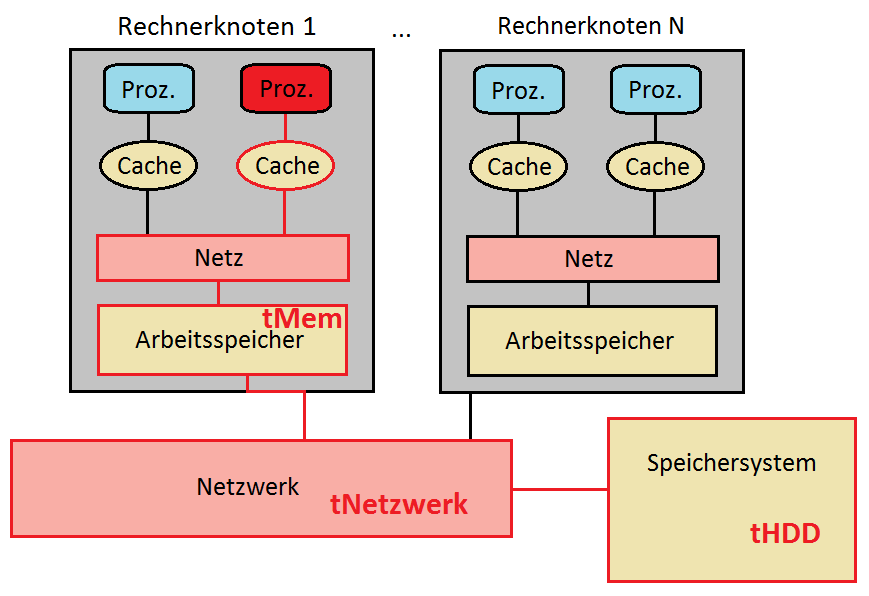
\includegraphics[width=.43\textwidth]{Bilder/rechnerknoten_ea_pfad.png}
	\end{center}
	\caption{E/A-Pfad im System; der rot gekennzeichnete Prozessor macht einen E/A-Zugriff, der Pfad führt entlang der roten Markierung}
	\label{fig:ea_pfad}
\end{figure}

Für einen Schreibzugriff gilt im Wesentlichen ein ähnlicher Ablauf.
Die Daten müssen beim Schreiben eigentlich immer über das Netzwerk auf Festplatte geschrieben werden. Dies ist nur dann nicht der Fall, wenn eine Caching-Strategie wie Write-Back genutzt wird. Dann wird die Datei nur im Hauptspeicher des Rechnerknotens geändert und erst später endgültig auf Festplatte geschrieben.
Der Datenfluss beim Schreiben fließt umgekehrt zu dem des Lesezugriffs.

\subsection{Faktoren der Zugriffszeit}
An allen Stationen des E/A-Pfades gibt es jeweils einen konstanten Anteil der Zugriffszeit und einen Anteil, der von der aufgerufenen Datei abhängt. 
Der Teil der Zugriffszeit, der für jeden Aufruf konstant ist, ist für die Modellierung weniger spannend und sollte bereits durch einfache lineare Modelle darstellbar sein, dieser Teil wird im Folgenden nicht weiter berücksichtigt.
Desweiteren kann es an verschiedenen Stellen zu Verzögerungen durch Wartezeiten (engl. queue times) für die Verarbeitung des E/A-Aufrufs kommen. Dieser Faktor ist nicht anhand des Attribut-Tupels bestimmbar und könnte höchstens durch eine Zeitreihenbetrachtung approximiert werden. Konstanter Verwaltungsaufwand und Wartezeiten können als Latenzzeit zusammengefasst werden. Die Latenz einer Station des E/A-Pfades ist also die Verzögerungszeit, bis die Datenübertragung angelaufen ist.\\
Im Folgenden sollen die Faktoren betrachtet werden, die im Wesentlichen von den bekannten Variablen des Attribut-Tupels abhängen.
Für beide Zugriffsarten ergeben sich die drei beschriebenen Zeitfaktoren tMem, tHDD und tNetzwerk.

\begin{itemize}
	\item Der netzwerkabhängige Teil tNetzwerk ist vom genauen Speicherort der aufgerufenen Datei, sowie der Größe der Datei abhängig. Der Faktor des Speicherorts im E/A-System sollte allerdings eine eher ungeordnete Rolle spielen, zudem sind keine Informationen darüber verfügbar; dieser Faktor wird daher vernachlässigt. 
	Der entscheidende Zeitfaktor entsteht durch die Übertragung der Daten über das Netzwerk. Der Datenfluss über das Netzwerk hängt von dessen Durchsatz ab, dieser sollte nach kurzer Verbindungsaufbauphase konstant sein.
	\item tMem ist am einfachsten zu modellieren, denn der hier auftretende Direktzugriffsspeicher (engl. Random-Access Memory) kennzeichnet sich gerade dadurch, dass der Zugriff auf alle Datenblöcke mit gleichem zeitlichen Aufwand verbunden ist.
	Ansonsten hängt die Zugriffszeit vom Durchsatz des Speichers ab.
	Eigentlich handelt es sich bei tMem um die Zusammensetzung der Zeitanteile von dem Arbeitsspeicher und den Caches. tMem wird im Modell jedoch vom langsamsten Speicher, der angesprochen werden muss, dominiert.
	\item Die Festplatte ist ähnlich komplex wie das Netzwerk. Wie beim Netzwerk ist die Zugriffszeit zum Einen von dem genauen Speicherort der angefragten Datenblöcke und zum Anderen vom Durchsatz der Festplatte abhängig.
	Die Zugriffszeit ist von der zu überwindenden Strecke, vom vorherigen Aufenthaltsort zum Zielort, des Lese-/Schreibkopfes abhängig.
	Diese erwartete Strecke hängt dabei mit dem $\mbox{Delta-Offset}$ zusammen, weil Dateisysteme versuchen Dateien möglichst zusammenhängend abzulegen.
	Ein großer Abstand der Zugriffsorte in der Datei sollte auch in einem größeren Abstand auf der Magnetscheibe der Festplatte resultieren.
	Der zeitliche Aufwand zum Überwinden des $\mbox{Delta-Offset}$ ist von den Hardwarecharakteristika der Festplatte abhängig. Ansonsten ist die Zugriffszeit linear von dem Durchsatz der Festplatte und der Größe des angefragten Abschnittes abhängig.
\end{itemize}

tMem müsste nach diesem Modell vollständig durch ein lineares Modell dargestellt werden können. Dagegen ist dies für tNetzwerk und tHDD nur bedingt der Fall.
Netzwerk und Festplatte haben einen je nach Zugriffsgröße dominierenden linearen Anteil, jedoch auch einen vom Speicherort abhängigen.
Die Durchsätze von tMem sowie tHDD sind hardwarebedingt von der Art des Zugriffs abhängig, es muss also zwischen Lese- und Schreibzugriffen unterschieden werden.
Dies geschieht über den Operationstyp (OpTyp).

Das Modell für die Ein-/Ausgabe in dieser Arbeit entspricht letztendlich:
\vspace*{-0.15cm}
\begin{align*}
\mbox{tGesamt} &= \mbox{tHDD} + \mbox{tNetzwerk} + \mbox{tMem}\\
\text{mit}\\
\mbox{tHDD} &= \frac{\mbox{Zugriffsgröße}}{\mbox{Festplattendurchsatz(OpTyp)}} + \mbox{Festplattenlatenz(Delta-Offset)} \\
\mbox{tNetzwerk} &= \frac{\mbox{Zugriffsgröße}}{\mbox{Netzwerkdurchsatz}} + \mbox{Netzwerklatenz}\\
\mbox{tMem} &= \frac{\mbox{Zugriffsgröße}}{\mbox{Speicherdurchsatz(OpTyp)}} + \mbox{Speicherlatenz}
\end{align*}

Alle Messungen zu Speicheraufrufen mit dem selben Attribut-Tupel hätten nach diesem Modell idealerweise dieselbe Laufzeit.

\subsection{E/A-Pfad zur Leistungsvorhersage}
\label{analyse:ea_pfad_zurvorhersage}
Anhand eines kurzen Vorgriffs auf die Messdaten-Exploration kann die Auswirkung des E/A-Pfades auf die Laufzeit der Messungen gezeigt werden.
In Abbildung \ref{fig:pfad_for_vorhersage} ist die Zugriffszeit für E/A-Zugriffe einer Messreihe gezeichnet. Alle Messungen derselben Farbe gehören zum selben Attribut-Tupel, ihre Aufrufparameter sind also gleich.\\
\begin{figure}[!bH]
	\begin{center}
		\subfloat{
			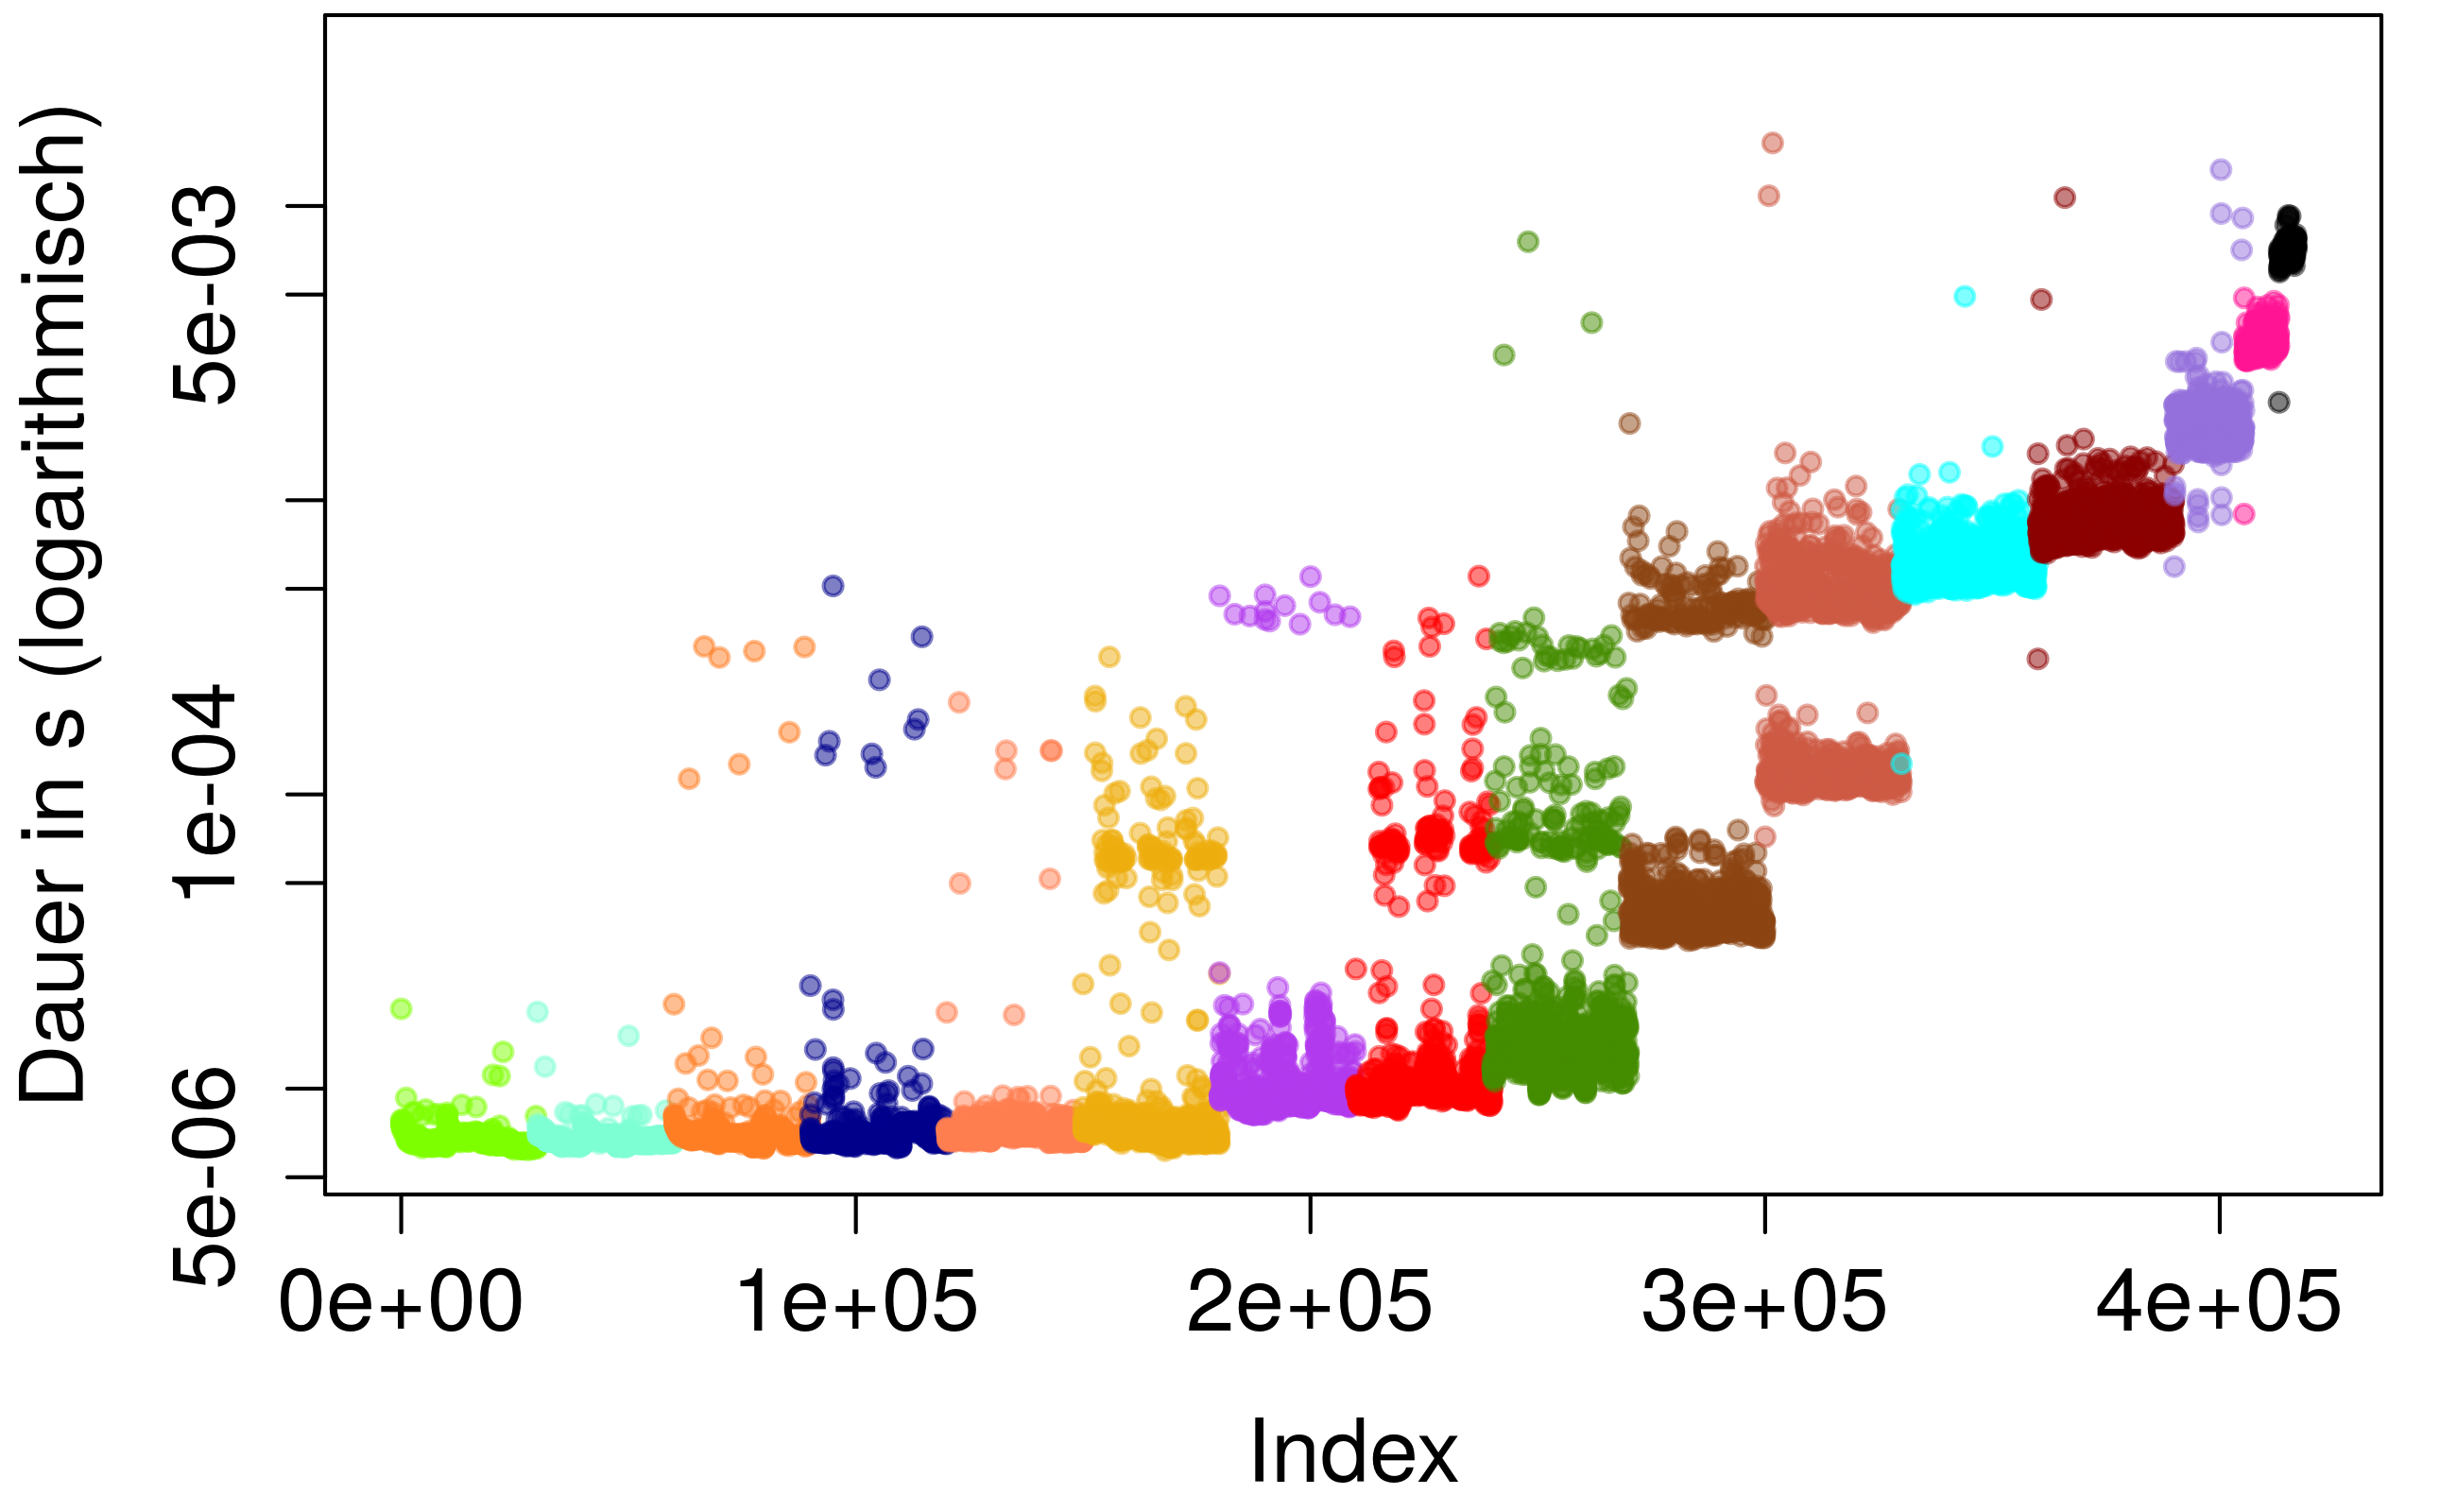
\includegraphics[width=.5\textwidth]{Bilder/Plots/exploration/plot_SizeSorted_log_read_seq.png}
		}
		\caption{Graphische Darstellung der Laufzeiten einer Messreihe mit lesenden E/A-Aufrufen. Jede Farbe repräsentiert eine Zugriffsgröße.}
		\label{fig:pfad_for_vorhersage}
	\end{center}
\end{figure}
In der Abbildung ist gut zu erkennen, dass die Zugriffszeiten in Stufen zunehmen.
Dies liegt einerseits an den in Intervallen ansteigenden Zugriffsgrößen der Messungen, kann aber andererseits auch der Zugehörigkeit der Messung zu einem E/A-Pfad zugesprochen werden.
Die Zugriffszeit eines Pfades wird von der langsamsten Komponente auf dem Weg dominiert.
Dadurch kann ein Sprung in der Laufzeit entstehen sobald sich der Pfad verlängert. Der Pfad verlängert sich, wenn auf eine tiefere Schicht der Speicherhierachie zugegriffen werden muss. Da die tieferen Schichten auch zunehmend langsamer werden, entsteht jedes mal ein Sprung in der Laufzeit.\medskip

In der Abbildung wird auch direkt klar, dass die Annahme fallengelassen werden muss, dass Messungen mit gleichem Attribut-Tupel dieselbe Laufzeit haben. Die Laufzeiten innerhalb von Messreihen zu gleichen Attributen unterscheiden sich teilweise deutlich.
Anhand dieser Verteilung kann die Abhängigkeit der Laufzeiten vom E/A-Pfad zu erkannt werden.
Wäre die Laufzeit im Wesentlichen nur vom Attribut-Tupel und dem \glqq zufälligen\grqq{} momentanen Systemzustand abhängig, dann sollten die Messungen zum selben Tupel in einer gleichmäßig verteilten Wolke aufzufinden sein.
Die Laufzeiten eines Attribut-Tupels weisen allerdings ein sprunghaftes Verhalten auf. Die dunkelgrünen Punkte sind beispielsweise in drei Gruppen aufgeteilt.
Die roten und violetten Messungen, links neben den dunkelgrünen, weisen ein ähnliches Muster auf, bei den violetten fehlt die mittlere Gruppe.
Die Zugriffsgröße der dunkelgrünen Messungen ist dabei vier mal höher (4\,KiB zu 16\,KiB).
Wie lange die Verarbeitung des E/A-Aufrufs dauert, scheint aber im Wesentlichen für die drei Attribut-Tupel gleich zu sein und vor Allem davon abzuhängen, in welcher Stufe sich der zugehörige Punkt der Messung befindet.\medskip

Die zuvor aufgestellte Modellierung kann die Abhängigkeit zwischen E/A-Pfad und Laufzeit nicht wiedergeben.
Jede Ebene der Speicherhierachie könnte hingegen modelliert werden, falls der E/A-Pfad also bereits bekannt wäre, könnte aus einer Komposition von Modellen für alle Pfade das korrekte ausgewählt werden.
Möglicherweise könnte eine Zeitreihenbetrachtung Hinweise über die Zugehörigkeit einer Messung zu einem Pfad geben. 

Ein perfektes Modell sollte unter Kenntnis des Pfades, den ein E/A-Aufruf nehmen wird, und dem Attribut-Tupel die Dauer des Zugriffs sehr gut vorhersagen können. Wenn das Modell nicht die Informationen über die E/A-Pfade erhält bzw. es nicht möglich ist  diese Kenntnisse aus anderen Attributen abzuleiten, kann es nicht zwischen den Gruppierungen innerhalb der Messungen eines Attribut-Tupels unterscheiden. Die Qualität der Vorhersagen ist damit begrenzt, die beste Näherung wäre dann die typische Laufzeit (bspw. das arithmetische Mittel) für alle Messungen eines Attribut-Tupels als Approximation der individuellen Laufzeit einer Messung zu nutzen.

\section{Validierung und Metriken}
\label{analyse:valid}
Mit den im Weiteren entwickelten Modellen soll untersucht werden, wie gut es gelingt, den zeitlichen Aufwand für E/A-Aufrufe vorherzusagen. 
Jedes Modell trifft bestimmte Annahmen über das E/A-System und zur Entwicklung einer Instanz des Modells werden bestimmte Informationen benötigt.
Diese benötigten Daten können aus den Messdaten über das System abgeleitet werden.
Ein Teil der Daten wird als Trainingsdatensatz zum Lernen genutzt, die restlichen Daten sind dem Modell unbekannt und bilden den Testdatensatz. Die Vorhersagen der Modelle zum Testdatensatz können dann mit den tatsächlichen Werten verglichen werden. Dies ist die \textbf{Leistungsvorhersage} vom Modell zum System. \medskip

Neben der Vorhersage der Leistung wird in den komplexeren Modellen auch versucht die Quantile 0.1 und 0.9 der Laufzeit pro Attribut-Tupel vorherzusagen. Der Wert des 0.1 Quantil gibt an, dass zu 10\% der Messungen zu einem Attribut-Tupel Laufzeiten gemessen wurden, die langsamer als dieser Wert waren, entsprechend gibt das 0.9 Quantil an, dass nur 10\% der Messungen zu diesem Attribut-Tupel schneller abgearbeitet wurden.\\
Die Modelle sagen also voraus, dass Messungen zu einem spezifischen Attribut-Tupel mit 80\%iger Wahrscheinlichkeit zwischen den von ihnen bestimmten 0.1 und 0.9 Quantil liegen.\medskip

Wenn die schnellsten und langsamsten $10\%$ der Messungen eines Attribut-Tupels als Ausreißer bezeichnet werden, können die Modelle mit Hilfe der Vorhersage dieser Quantile eine Klassierung in Ausreißer und Nicht-Ausreißer machen. Diese Zuordnung wird als \textbf{Ausreißervorhersage} bezeichnet.
Bei den Ausreißern handelt es sich in diesem Kontext nicht um ungültige Messungen, die durch einen fehlerhaften Versuchsaufbau oder durch Fehlkalibrierung von Messinstrumenten entstanden sind. Stattdessen kann es beispielsweise sein, dass das System punktuell sehr ausgelastet war und die Latenzen dadurch ungewöhnlich hoch waren. 
Bei der Ausreißervorhersage wird geprüft, ob das Modell korrekt voraussagen kann, dass die Laufzeit einer E/A-Anfrage zu den Ausreißern gehört. Da es sich bei den Ausreißern nicht um Messfehler handelt ist eine solche Vorhersage prinzipiell möglich, wenn E/A-Pfad und Systemzustand bekannt sind.
Man könnte die Ausreißervorhersage auch als Test auf den schwierigsten Daten ansehen. 

Es würde für die Qualität eines Modells sprechen, wenn es sowohl eine gute Leistungsvorhersage, auch eine gute Ausreißervorhersage macht.

\subsubsection{Metriken zur Leistungsvorhersage}
Zur Analyse der Leistungsvorhersage nutze ich folgende Fehlermetriken:
\begin{itemize}
	\item Der \textit{\textbf{MAE}} (vom englischen \textit{mean absolute error}) ist der arithmetische absolute Fehler gemittelt über alle Vorhersagen.
	\item Der \textit{\textbf{MAPE}} (vom englischen \textit{mean absolute percentage error}) ist der relative \textit{MAE}, also der \textit{MAE} auf dem relativen Fehler der Vorhersage gegenüber der tatsächlichen Laufzeit.\\
\end{itemize}
\textit{MAE} und \textit{MAPE} geben eine Vorstellung davon, welchen Fehler man bei einer Vorhersage erwarten kann.
\begin{itemize}
	\item Um ein Verständnis für die Streuung der Modellabweichungen zu bekommen ist der quadratische relative Fehler gemittelt über alle Vorhersagen \textit{\textbf{MSPE}} (vom englischen \textit{mean square percentage error}) nützlich.
\end{itemize}
	Eine geringe quadratische Abweichung lässt darauf schließen, dass das Modell zuverlässig ist und nicht auf einem Teil der Messungen genau und für andere Messungen ungenau vorhersagt.\\
	Für denselben Zweck sind \textit{RQ3} und \textit{RMax} nützlich.
\begin{itemize}
	\item \textit{\textbf{RQ3}} gibt das obere Quartil des relativen Fehlers über alle Vorhersagen an.
	\item \textit{\textbf{RMax}} entspricht dem größten relativen Fehler der vom Modell gemacht wurde.
\end{itemize}
Wenn überprüft werden soll, ob die Vorhersagen eines Modells zumindest für die jeweiligen Attribut-Tupel sinnvoll oder vielleicht doch eher konservativ waren, kann der \textit{In-range} betrachtet werden.
\begin{itemize}
	\item Der Wert von \textit{\textbf{In-range}} gibt an wie viele der gemachten Vorhersagen zwischen dem 0.1 und 0.9 Quantil der Laufzeiten aller Messungen eines Attribut-Tupels lagen.
	Wenn alle Laufzeiten exakt vorhergesagt werden würden, wäre \textit{In-range} also bei 80\%. Wenn ein Modell konservativ vorhersagt, beträgt der \textit{In-range} 100\%, also liegen alle prognostizierten Werte zwischen den Quantilen, dass Modell \glqq versucht\grqq{} nicht Ausreißer vorherzusagen, sondern approximiert mit einer Art typischen Laufzeit. 
	Wenn der \textit{In-range} sehr klein oder gar 0 beträgt, macht das Modell keine sinnvollen Vorhersagen, denn die meisten vorhergesagten Laufzeiten lagen außerhalb der typischen Zugriffszeit der Attribut-Tupel.
\end{itemize}
Zwei zusätzliche Fehlermetriken enthalten weitere nützliche Informationen über die Netze, sodass die Leistung besser eingeordnet werden kann.

\begin{itemize}
	\item \textit{\textbf{Avg-MAPE}} (\textit{average} \textit{MAPE}) gibt den durchschnittlichen \textit{MAPE}-Wert für 12 Netze an. 
	Aufgrund der zufälligen Initialisierung und der lokalen Konvergenz durch das verwendete Gradientenverfahren sind die neuronalen Netze nicht deterministisch bestimmt.
	Je nachdem mit welchen Gewichten das Netz startet, ist das Ergebnis des Lernalgorithmus besser oder schlechter. Um falsche Schlussfolgerungen über die Qualität der Parameter zu verhindern, werden daher jeweils 12 Instanzen mit den gleichen Parametern und Trainingsdaten, aber mit unterschiedlicher Initialisierung, berechnet.
	Anhand des \textit{Avg-MAPE} kann die Auswirkung der lokalen Konvergenz für die jeweiligen Netzstrukturen betrachtet werden.
	\item Zusätzlich wird \textit{\textbf{Train-MAPE}} angegeben. Dies ist der erreichte \textit{MAPE}-Wert des Netzes auf den eigenen Trainingsdaten. Dieser Wert sollte immer besser als der normale \textit{MAPE} sein. Anhand der Differenz zu \textit{MAPE} kann beurteilt werden, wie gut die Trainingsdaten die Testdaten repräsentiert haben.
\end{itemize}

\subsubsection{Metriken zur Ausreißervorhersage}
Zur Evaluierung der Ausreißervorhersage werden weitere Fehlermetriken genutzt.\medskip

Die ersten Fehlermetriken beziehen sich auf die Vorhersagen der Laufzeit-Quantile. Idealerweise sollte das Modell jeweils die gleichen Werte für die Quantile zu jedem Attribut-Tupel vorhersagen, der möglichst nah am tatsächlichen Wert liegt, denn die Quantile beziehen sich auf jeweils alle Messungen zu einem Attribut-Tupel.
\begin{itemize}
	\item Die arithmetischen Mittelwerte über den relativen Fehlern (\textit{\textbf{Q0.1-MAPE}} und \textit{\textbf{Q0.9-MAPE}}).
	\item Die mittleren quadratischen Abweichungen über die relativen Fehler (\textit{\textbf{Q0.1-MSPE}} und \textit{\textbf{Q0.9-MSPE}}).
\end{itemize}
Zudem werden zwei Metriken einbezogen, die gemeinsam die Klassierung der Messungen in Ausreißer und Nicht-Ausreißer bewerten können.
\begin{itemize}
	\item \textit{\textbf{TP}} gibt den Anteil der korrekt vorhergesagten Ausreißer an, dies sind die richtig positiven Zuordnungen (engl. \textit{true positives}). Dieser Wert sollte möglichst hoch sein.
	\item \textit{\textbf{FP}} gibt dagegen die Anzahl Messungen an, die fälschlicherweise als Ausreißer eingestuft wurden (engl. false positives). Dieser Wert sollte gering gehalten werden.
\end{itemize}
Es ist wichtig, sowohl \textit{TP} als auch \textit{FP} zu betrachten. Ein Netz, das einfach alle Messungen als Ausreißer deklariert, würde einen perfekten \textit{TP}-Wert von 100\% erreichen, obwohl mit der Ausreißer-Bestimmung nichts anzufangen ist.

\section{Modellklassen}
\label{analyse:modellklassen}
Modelle unterscheiden sich einerseits anhand der Informationen, die ihnen über die E/A-Messungen zur Verfügung stehen, dies sind ihre Eingabeattribute, und andererseits an der zugrunde liegenden mathematischen Struktur.
Da es sich bei der E/A-Leistungsvorhersage um ein komplexes Problem handelt, steht nicht a priori fest, wie eine passende Modellierung auszusehen hat. 
In dieser Arbeit wurden daher verschiedene Ansätze getestet.

Aufgrund der Vielzahl verschiedener Modelle wird eine Einteilung in Modellklassen vorgenommen. Jede Klasse entspricht einem Ansatz, also einer bestimmten Herangehensweise ans Problem.
Die verschiedenen Modellklassen werden in den folgenden Kapiteln näher erläutert.

\subsection{Referenzmodelle}
Referenzmodelle werden auf einfache Weise mit klassischen mathematischen Methoden mit relativ geringem Rechenaufwand berechnet.
Das Ziel bei den Referenzmodellen ist nicht hauptsächlich die Qualität der Vorhersagen zu untersuchen, sondern verschiedene Ansätze zu erkunden und Vergleichswerte für komplexere Modelle zu liefern.
Einige Referenzmodelle stellen eine untere Schranke für die Vorhersagequalität der aufwendigeren Modelle dar. Andere zeigen auf, was bestenfalls mit einem Ansatz erreichbar ist.
Beispielsweise kann an den Ergebnissen eines Modells, das bloß lineare Zusammenhänge beschreiben kann, untersucht werden, ob die Daten in linearer Weise beschrieben werden können.\medskip

Bei Referenzmodellen wird nicht zwischen Trainings- und Testdaten unterschieden, sie werden immer über die gesamten Messdaten trainiert und ausgewertet.
Eine Separation der Datensätze ist für beide Verwendungszwecke der Referenzmodelle nicht sinnvoll. 
Wenn untersucht werden soll, ob ein lineares Modell die Messdaten beschreiben kann, sollte der gewählte Trainingssatz nicht eingeschränkt werden, ebenso wenn gezeigt werden soll, wie gut ein Konzept bestmöglich sein kann.

\subsection{NN-Modelle}
Das Hauptaugenmerk der Arbeit liegt auf der Anwendung von künstlichen neuronalen Netzen zur Leistungsvorhersage der E/A-Zugriffe. Die Modelle, die auf neuronalen Netzen basieren, werden als NN-Modelle bezeichnet.
Die Erwartungshaltung ist, dass NN-Modelle wesentlich bessere Ergebnisse erzielen, als die Referenzmodelle, die untere Schranken für die Leistung definieren.
Wenn dies nicht der Fall ist, war entweder die Modellierung unzureichend oder die verwendeten Informationen über die Messdaten waren unzureichend für eine gute Beschreibung des E/A-Systems.\medskip

Bei NN-Modellen gibt es die Aufteilung zwischen Trainings- und Testdatensatz.
Sie könnten daher auch in einer realen Anwendungssituation genutzt werden. 
Bei der tatsächlichen Anwendung eines E/A-Leistungsprädiktors wäre es nicht möglich, dass das Modell bereits sämtliche E/A-Aufrufe gesehen hat, deren Laufzeiten es vorhersagen soll.

\subsection{Fehlerklassen-Modelle}
\label{fk-modelle}
Fehlerklassen (\textbf{FK}) werden mit Hilfe der Vorhersagen eines anderen Modells berechnet. Der Fehler (auch Residuum oder Modellabweichung) der Vorhersagen gegenüber den tatsächlichen Laufzeiten der E/A-Aufrufe wird mit dem k-Means-Algorithmus (siehe Kapitel \ref{back_ML}) in 10 Cluster unterteilt.
Jede Cluster-Gruppe entspricht einer Klasse und bekommt eine Nummer. 
Die Klassen repräsentieren unterschiedliche Pfade, die im E/A-System genommen wurden. Dies ist dann der Fall, wenn das Modell, mit dem die Fehlerklassen erstellt wurden, bereits recht gute Vorhersagen macht und somit den \textit{üblichen} E/A-Pfad des Attribut-Tupels richtig bestimmt. 
Ein gutes Modell, das nicht zwischen Fehlerklassen unterscheidet, würde beispielsweise zu den gleichfarbigen Punkten in Abbildung \ref{fig:pfad_for_vorhersage} die mittlere Laufzeit aller zugehörigen Messungen vorhersagen, oder vielleicht allen eine Laufzeit aus der Gruppe mit den meisten Punkten zuordnen. 
Der dabei gemachte Fehler gegenüber den tatsächlichen Laufzeiten ist dann charakteristisch für die Sprünge, die bei den Übergängen der Pfade beobachtet wurden.
Wenn zum Beispiel zu den dunkelgrünen Punkten jeweils ein Wert aus der mittleren Gruppe von Messungen vorhergesagt werden würde, so würde ein sehr kleiner Fehler eine Zugehörigkeit zum dort genommenen E/A-Pfad repräsentieren.
Ein größerer negativer oder positiver Fehler würde darauf hinweisen, dass bei diesem Aufruf ein entsprechend anderer Pfad genommen wurde.\\
Die Schätzung ist, dass das System pro Anwendungsfall etwa 10 verschiedene E/A-Pfade nutzt, daher werden die Messungen in 10 Gruppen aufgeteilt.\medskip

Es muss beachtet werden, dass Modelle, die Fehlerklassen ausnutzen, keine verwendbaren Prädiktoren zur Leistungsvorhersage ergeben.
Dies liegt daran, dass die tatsächlichen Laufzeiten der Messungen im Testdatensatz für Modelle mit Fehlerklassen bekannt sein müssen. 
Mit Hilfe der tatsächlichen Laufzeiten können die Modellabweichungen zu einem anderen Modell berechnet werden, die für die Zuordnung in Fehlerklassen benötigt werden.\medskip

Die Fehlerklassen-Modelle werden stattdessen untersucht, um die Aussagekraft von E/A-Pfaden zu analysieren.
Wenn E/A-Pfade charakteristisch für die Zugriffszeiten sind, dann sollten diese Modelle eine wesentlich geringere Modellabweichung aufzeigen als Modelle ohne Fehlerklassen.

Sowohl Referenzmodelle als auch NN-Modelle werden im Folgenden entwickelt und untersucht.
\subsection{Aufbereitung der Trainingsdaten}
Die Eingabedaten der Modelle können auf zwei grundsätzlich verschiedene Weisen aufbereitet werden.
Entweder werden einem Modell Informationen zu einzelnen Messungen nach und nach gegeben oder jeweils eine Teilmenge der Trainingsdaten werden als Aggregate zusammengefasst.\medskip

Das Problem bei Einzelmessungen ist, dass \glqq widersprüchliche\grqq{} Angaben zur Laufzeit von Messungen mit gleichen Parametern gemacht werden. Es kann sehr viele Messungen mit gleichen Parametern geben, solange nur die Attribute Zugriffsgröße, Delta-Offset und OpTyp genutzt werden . 
Für die Aggregate werden bestimmte Attribute definiert und alle Messungen mit identischen Werten zu allen diesen Attributen werden zusammengefasst.
Der Wert für die Laufzeit eines Aggregats ergibt sich dann beispielsweise als arithmetischen Mittelwert oder Median über alle zugehörigen Messungen.
Die Modelle, die nur aggregierte Eingabedaten nutzen, vereinfachen das Problem entsprechend sehr stark. Sie verfolgen den Ansatz, dass es mit den gegebenen Informationen nicht möglich ist, innerhalb eines Attribut-Tupels zu differenzieren, sodass verschiedene Messungen eines mit denselben Attributen alle dieselbe Vorhersage zugewiesen bekommen.

Modelle, die Einzelmessungen als Eingabe bekommen, müssen anders mit den \glqq widersprüchlichen\grqq{} Informationen umgehen.
Das Modell muss dann entweder intern die Daten zusammenfassen, um doch dieselbe Vorhersage für jede Messung eines Attribut-Tupels zu machen oder es versucht anhand weiterer Informationen über den Systemzustand eine Differenzierung durchzuführen.
Die zweite Lösung entspricht der Zeitreihenbetrachtung.
Modelle, die eine Zeitreihenbetrachtung machen, brauchen die (zeitlich sortierten) Einzelmessungen als Eingabe, da bei der Aggregierung alle zeitabhängigen Informationen verloren gehen.
Sie können dafür versuchen, ein periodisches Systemverhalten zu erkennen und dieses für ihre Vorhersage auszunutzen. So könnte es beispielsweise sein, dass jeder dritte Leseaufruf doppelt so lange wie die vorherigen dauert, weil das E/A-System zunächst einem anderen Prozess Priorität gibt.
Wenn ein solches Verhalten erkannt wird, könnte die Vorhersage durch so ein Modell erheblich verbessert werden.

\section{Untersuchte Modelle}
\label{analyse:modelle}
Bevor die Modelle entwickelt wurden, die in dieser Arbeit untersucht werden sollen, wurden die Messdaten exploriert, um zu verstehen, welche Attribute zu den Messungen interessant sind.
Wenn es darum geht, gute Attribute für die Modelle zu finden, kann die Korrelation des Attributs zu den Laufzeiten der Messungen betrachtet werden.
Die Korrelation ist ein Wert zwischen 0 und 1, und ist ein Maß für den linearen Zusammenhang zweier Variablen. Eine Korrelation von 0 besagt, dass die Information über eine der Variablen keinen linearen Zusammenhang zur Anderen hat.
Bei einer Korrelation von 1 dagegen, kann eine lineare Funktion angegeben werden, aus der sich der Wert der einen Variablen direkt der Wert der Anderen berechnen lässt. Somit ist eine hohe Korrelation zwischen einem Attribut eines E/A-Aufrufs und dessen Laufzeit ein Hinweis darauf, dass dieses Attribut zur Vorhersage der Laufzeit verwendet werden könnte. 
Allerdings wird bei der Korrelation bloß die lineare Abhängigkeit betrachtet, ein komplexerer Zusammenhang zweier Variablen wird dadurch schlecht oder gar nicht repräsentiert.
Abgesehen von der Korrelation war Expertenwissen ausschlaggebend für die Wahl der verwendeten Attribute für jedes Modell.

Ich stelle nun kurz alle Modelle vor, die untersucht wurden. Zunächst gehe ich die Referenzmodelle durch, dann die NN-Modelle.\\
Eine Kurzbeschreibung der Modelle ist für die Referenzmodelle in Tabelle \ref{tab:zusammenfasssung_referenz} und für NN-Modelle in Tabelle \ref{tab:zusammenfasssung_nn} gegeben.

\subsection{Referenzmodelle}
\begin{table}
	\centering
	\scriptsize
	\subfloat{
		\begin{tabular}{|r|p{4.6cm}|p{4.4cm}|p{3.2cm}|}\hline%
			\textbf{Modell} & \textbf{Beschreibung}  & \textbf{Art der Trainingsdaten} & \textbf{Benötigte Attribute zur Vorhersage}\\\hline\hline
			\csvreader[late after line=\\\hline, separator=semicolon]%
			{CSV/zusammenfassung_der_referenz_modelle.csv}{Modell=\Modell, Beschreibung=\Beschreibung, Art=\Art, Attribute = \Attribute}%
			{\Modell & \Beschreibung & \Art & \Attribute}%
		\end{tabular}
	}
	\label{tab:zusammenfasssung_referenz}
	\caption{Kurzbeschreibungen der Referenzmodelle}
\end{table}
\begin{itemize}
	\item Das einfachste Modell ist \textit{\textbf{Durchschnitt}} das Modell approximiert alle Laufzeiten mit dem globalen arithmetischen Mittelwert der Laufzeiten.
Da das Modell überhaupt nicht auf die Attribute der betrachteten Messungen eingeht, sollten alle Modelle, die dies tun, bessere Leistungen erbringen. Einem Modell, das diese Informationen ausnutzt und dennoch schlechtere Leistungen erzielt, könnte unterstellt werden, im Wesentlichen zufällige Vorhersagen zu machen.
\textit{Durchschnitt} ist als untere Schranke für alle NN-Modelle gedacht.
	\item Eine ähnliche Methode wie \textit{Durchschnitt} verwendet das Modell \textit{\textbf{Median agg}}. Es berechnet für jedes Attribut-Tupel den Median der Laufzeiten, dieser Wert entspricht dann der Vorhersage des Modells für Messungen zu diesem Attribut-Tupel.
Dieses Modell ist eine Referenz dazu, wie gut die Modellierung eines Modells, das nicht nicht zwischen verschiedenen Messungen zum selben Attribut-Tupel unterscheiden kann, bestmöglich sein kann.
	\item Lineare Regression ist ein einfaches numerisches Verfahren, das eine lineare Funktion berechnet, die den quadratischen Fehler zu den bekannten Messpunkten minimiert (Methode der kleinsten Quadrate).
Die Funktion ist eine Gerade der Form $f(x) = a + b \cdot x$, mit der Verschiebung $a$ und Steigung $b$. Wird die Regression über mehrere Variablen gemacht erhält man Verschiebungen und Steigungen, die sich aus den Komponenten zu jeder Variable zusammensetzen.
Ich probiere drei verschiedene lineare Modelle aus.
\textit{\textbf{LinReg G}} wird nur aus dem Zusammenhang von Zugriffsgröße und Laufzeit berechnet.
\textit{\textbf{LinReg G+D}} enthält auch die Werte zu Delta-Offset und \textit{\textbf{LinReg G+D+O}} berücksichtigt zudem den Operationstyp der Messungen.
Die Modelle können wegen der linearen Form nicht innerhalb eines Attribut-Tupels unterscheiden. Sollte das vermessene E/A-System bereits durch lineare Zusammenhänge in den gemessenen Informationen beschreibbar sein, so sollten diese Modelle gute Ergebnisse zeigen.
\textit{LinReg G} wird einmal mit Einzelmessungen als Eingabe berechnet und einmal mit aggregierten Eingabedaten, dabei wird über alle Attribute des Attribut-Tupels (Zugriffsgröße, Delta-Offset und OpTyp) aggregiert. 
Da die quadratische Abweichung des berechneten linearen Modells zu allen Eingabedaten minimiert wird, findet bei der Einzelmessungs-Eingabe eine Gewichtung nach Häufigkeit des Auftretens eines Attribut-Tupels statt.
	\item Zuletzt gibt es noch zwei Fehlerklassen-Modelle. Die Eingabedaten sind aggregiert nach dem Attribut-Tupel und den Fehlerklassen. 
Sie funktionieren also genauso wie \textit{Median agg}, nur dass die Messungen zusätzlich noch durch ihre Fehlerklasse unterschieden werden. Es wird also der Median für alle Messungen eines Attribut-Tupels berechnet, die zur selben Fehlerklasse gehören.
\textit{\textbf{LinRegFK Median agg}} kennt die Fehlerklassen, die aus der Clusteranalyse der Fehler von \textit{LinReg G} gewonnen wurden, und \textit{\textbf{Tupel1FK Median agg}} modelliert mit Hilfe der Klassen, die aus den Modellabweichungen der besten Instanz von \textit{NN-Tupel1} (wird im Folgenden Abschnitt über die NN-Modelle erklärt) berechnet wurden.
\end{itemize}

\subsection{NN-Modelle}
Die weiteren Modelle sind NN-Modelle, es handelt sich hierbei um neuronale Netze, die sich anhand der Eingabeattribute unterscheiden.

\begin{itemize}
	\item Das Modell \textit{\textbf{NN-Tupel1 agg}} ist das Analogon der NN-Modelle zu \textit{Median agg}. Das Modell kennt allerdings, so wie alle NN-Modelle, nur einen Ausschnitt der Messdaten.
	Im Gegensatz zum zuvor betrachteten Idealfall muss das Modell die Laufzeiten unbekannter Messattribute interpolieren.
	Der Eingabevektor, den das neuronale Netz zu jedem Aggregat erhält, beinhaltet die Werte zu allen Attributen des Attribut-Tupels, nach welchen die Trainingsdaten auch aggregiert wurden.
	Das Netz versucht dann also das Tripel $(\mbox{Zugriffsgröße}, \mbox{Delta-Offset}, \mbox{Operationstyp})$ in Relation zum zugehörigen Median der Laufzeiten zu bringen.
	Das Modell muss sich nicht nur die Mediane der Laufzeiten zu den Attribut-Tupeln \textit{merken}, sondern möglichst gut die Zusammenhänge zwischen den Attribut-Werten und den zugehörigen Laufzeit-Mediane bestimmen, um unbekannte Attribut-Tupels sinnvoll vorhersagen zu können.
	\item Ganz ähnlich wie \textit{NN-Tupel1 agg} ist das Modell \textit{\textbf{NN-Tupel1}} aufgebaut. Die Eingabedaten werden allerdings nicht aggregiert.
	Es versucht also direkt, das beschriebene Tripel auf die zugehörigen Laufzeiten abzubilden. Es erhält sonst keine weiteren Informationen, sodass es ebenso wenig wie das aggregierende Modell zwischen Messungen mit gleichen Attributen unterscheiden kann.
	Es muss dann selbständig einen Mittelwert zu jedem Attribut-Tupel bilden und mit diesem assoziieren.
\end{itemize}
	\begin{figure}
		\centering
		\subfloat[Skizze von \textit{NN-Tupel1 agg}]{
			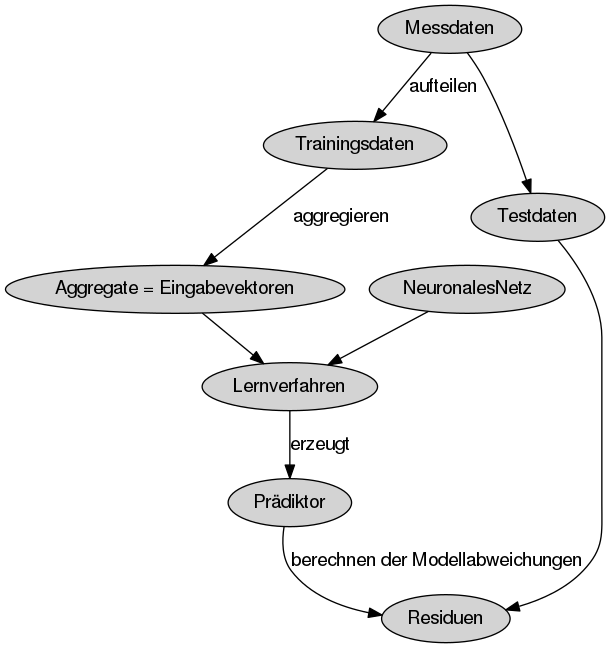
\includegraphics[width=.5\textwidth,height=.5\textwidth]{Dot/tupel1agg.png}
		}
		\subfloat[Skizze von \textit{NN-Tupel1}]{
			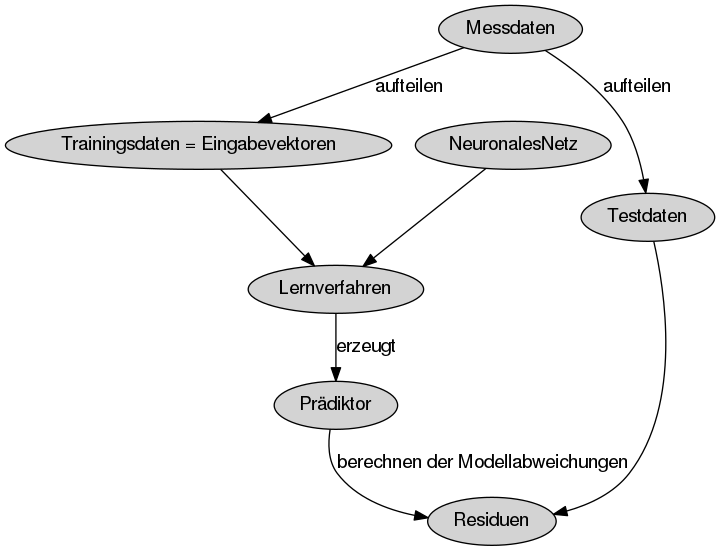
\includegraphics[width=.5\textwidth,height=.5\textwidth]{Dot/tupel1.png}
		}
		\caption{Vergleich der Erstellung und Anwendung von \textit{NN-Tupel1 agg} (links) und \textit{NN-Tupel1}(rechts)}
		\label{fig:tupel1vstupel1agg}
	\end{figure} 
\begin{itemize}
	\item \textit{\textbf{NN-Tupel2}} ist das erste Modell, das die zeitliche Reihenfolge der Messungen ausnutzen soll. Das neuronale Netz bekommt nicht nur die Werte zum Attribut-Tupel der Messung, deren Leistung es vorhersagen soll, sondern auch die zum Attribut-Tupel und die Laufzeit der vorherigen Messung.
	Die Idee hierbei ist, dass anhand des Wissens, wie schnell die letzte E/A-Prozedur bearbeitet werden konnte, eine Aussage über die nächste getroffen werden kann. Falls das System beispielsweise gerade besonders ausgelastet ist, sollte sich dies an der Laufzeit des vergangenen E/A-Aufrufs zeigen.
	Es könnte auch sein, dass das System eine sehr simple Periodizität aufweist, sodass nach einer schnellen Bearbeitung eine langsame folgt oder Ähnliches.
	\item Eine tieferliegende Periodizität könnte unter Umständen durch \textit{\textbf{NN-EMA}} für die Vorhersage der Laufzeit ausgenutzt werden. Die Grundlage für dieses Modell bildet die exponentielle Glättung (im englischen \textit{exponentiell moving average} (EMA)). In der Signalverarbeitung wird der EMA als Tiefpassfilter mit unendlicher Impulsantwort bezeichnet.
	Mit dessen Funktionswert kann ein Einblick in den generellen Trend der Zeitreihe gewährt werden, da temporäre Spitzen geglättet werden.
	Die Idee dieses Verfahrens ist, dass der kommende Zeitreihenwert im Wesentlichen von den direkten Vorgängern beeinflusst wird; in einem geringeren Maße jedoch auch von weiter zurückliegenden Messungen.
	In dem hier betrachteten Fall könnte das beispielsweise bedeuten, dass ein E/A-Aufruf gemacht wurde, der Speicherblöcke angefragt hat, die über das Netzwerk zum Rechnerknoten geholt werden müssen. Da das Netzwerk jedoch gerade durch andere Zugriffe ausgelastet ist, hat der Aufruf ungewöhnlich lange gedauert. Nun werden ein paar Aufrufe innerhalb des eigenen Arbeitsspeichers gemacht, die eine normale Laufzeit aufweisen. Über den aktuellen Wert der exponentiellen Glättung besteht noch eine Erinnerung an das langsame Verhalten vor einigen E/A-Aufrufen, sodass die Vorhersage zu einem erneuten Zugriff über das weiterhin ausgelastete Netzwerk präziser gemacht werden könnte.
	Um die Auslastung des E/A-Systems sinnvoll wiederzugeben, wird der Durchsatz der Messungen für die exponentielle Glättung genutzt. Der Durchsatz berechnet sich als $\mbox{Durchsatz} =  \frac{\mbox{Zugriffsgröße}}{\mbox{Laufzeit}}$.
	
	Karardzic definiert den EMA rekursiv \cite{kantardzic2011data} (S. 40):
	\begin{align*}
	EMA(i,m) &= p \cdot t(i)+(1-p) \cdot EMA(i-1,m-1)\\
	EMA(i,1) &= t(i)
	\end{align*}
	Dabei ist $p$ also die Gewichtung für den direkten Vorgängerwert und $1-p$ die Gewichtung für alle vergangenen Werte, $i$ ist der aktuelle Messwert und es werden die letzten $m$ Messungen berücksichtigt. Nummerieren wir alle Messungen von 1 bis $n$ durch und berücksichtigen immer alle bisherigen Messungen, also $i = m$, so sind die ersten Werte:
	\begin{align*}
	EMA(1,1) &= t(1)\\
	EMA(2,2) &=  p \cdot t(2)+(1-p) \cdot t(1)\\
	EMA(3,3) &=  p \cdot t(3)+(1-p) \cdot (p \cdot t(2)+(1-p) \cdot t(1))
	\end{align*}
	Der Eingabevektor des neuronalen Netzes \textit{NN-EMA} enthält alle Attribute des Attribut-Tupels, zusätzlich beinhaltet er den EMA mit $p=0.5$ der vergangenen Durchsätze.
	\item Abschließend gibt es analog zu den trivialen Modellen auch zwei NN-Modelle, die mit Fehlerklassen arbeiten.
	Die beiden Modelle bekommen das Attribut-Tupel der Messungen und zudem deren Fehlerklasse als Eingabeattribute.
	\textit{\textbf{NN-LinRegFK}} mit den Fehlerklassen die aus den Residuen des Referenzmodells \textit{LinReg G} berechnet wurden und \textit{\textbf{NN-Tupel1FK}} mit den Fehlerklassen, die aus den Ergebnissen der \textit{Tupel1} Instanz mit geringstem MSPE-Wert berechnet wurden.
\end{itemize}

\begin{figure}
	\centering
	%\subfloat[Skizze von NN-LinRegFK]{
	%	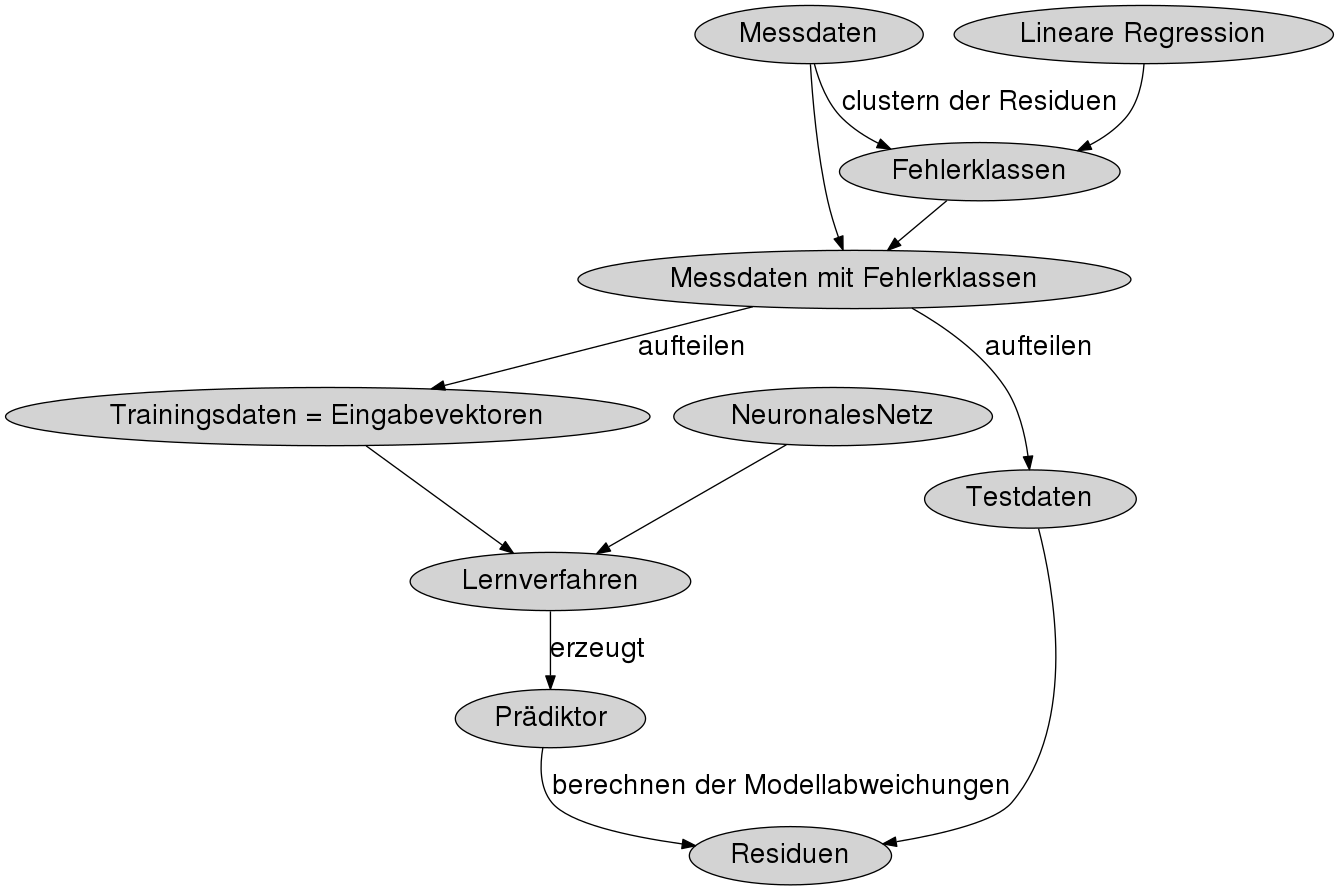
\includegraphics[height=.6\textwidth]{Dot/linregfk.png}
	%}\\
	\subfloat[Skizze von NN-Tupel1FK]{
		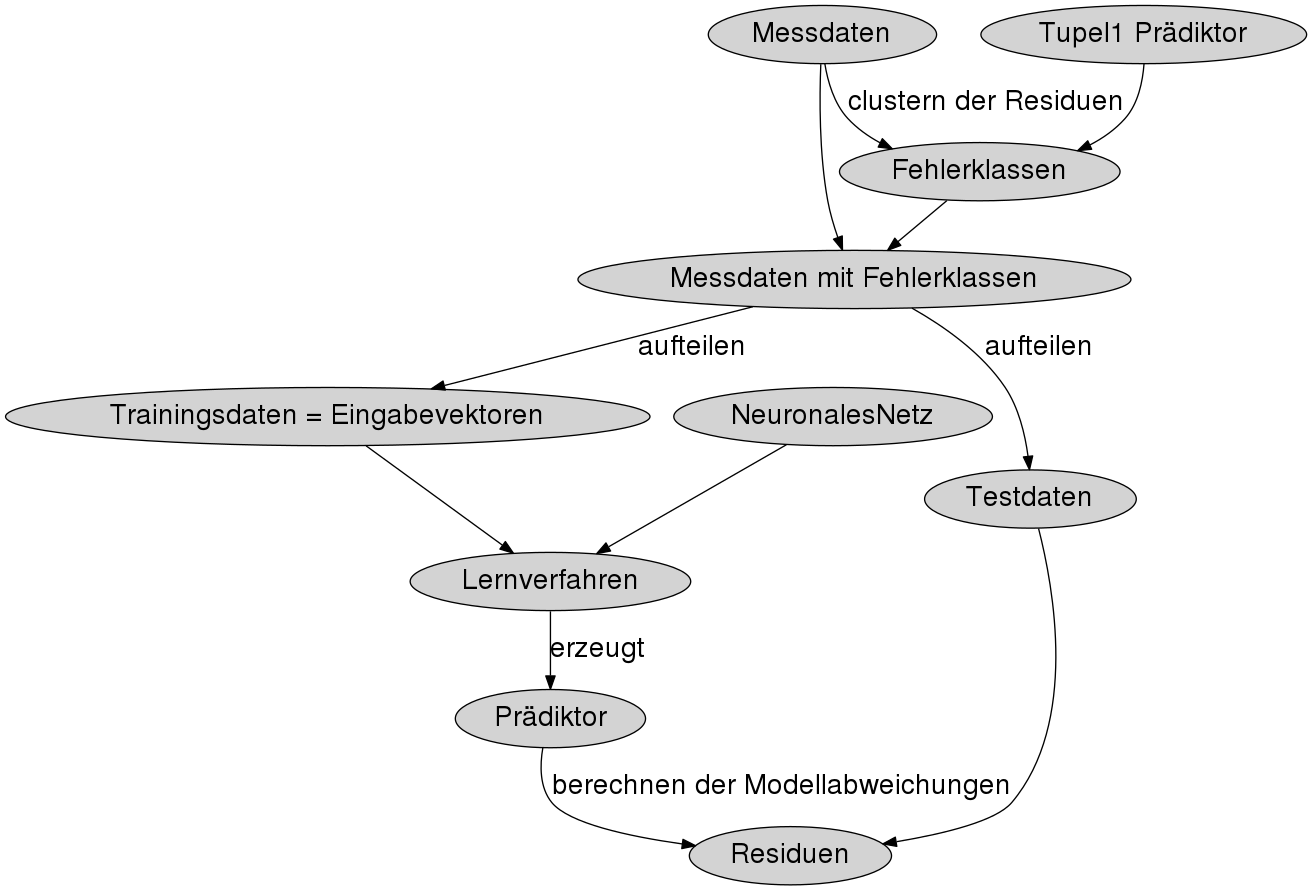
\includegraphics[height=.6\textwidth]{Dot/tupel1fk.png}
	}
	\caption{Erstellung und Anwendung von NN-Tupel1FK. NN-LinRegFK nutzt statt dem aus Tupel1 gewonnenen Prädiktor lineare Regression zum Erstellen der Fehlerklassen.}
	\label{fig:linregfkvstupel1fk}
\end{figure}

\begin{table}
	\scriptsize
	\subfloat{
		\hspace*{-0.9cm}
		\begin{tabular}{|r|p{4.6cm}|p{4.0cm}|p{3.2cm}|}\hline%
			\textbf{Modell} & \textbf{Beschreibung}  & \textbf{Art der Trainingsdaten} & \textbf{Attribute des Eingabevektors}\\\hline\hline
			\csvreader[late after line=\\\hline, separator=semicolon]%
			{CSV/zusammenfassung_der_NN_modelle.csv}{Modell=\Modell, Beschreibung=\Beschreibung, Art=\Art, Attribute = \Attribute}%
			{\Modell & \Beschreibung & \Art & \Attribute}%
		\end{tabular}
	}
	\label{tab:zusammenfasssung_nn}
	\caption{Kurzbeschreibungen der der NN-Modelle. Diese basieren auf neuronalen Netzen und bilden den Eingabevektor auf die Laufzeit ab.}
\end{table}

\section{Parametrisierung von NN-Modellen}
\label{parametrisierung}
Für die Referenzmodelle ist das Training durch einfache Berechnungen eindeutig definiert.
Bei den NN-Modellen hingegen müssen zunächst die Parameter der verwendeten neuronalen Netze festgelegt werden. 
Während manche Parameter durch Heuristiken oder nach einigen Testdurchläufen schnell ermittelt werden können, sind andere stark abhängig von den tatsächlichen Trainingsdaten, der Anzahl Datenpunkte und den verwendeten Attributen. Für das Lernverfahren eines neuronalen Netzes müssen eine Fehlerfunktion, eine Aktivierungsfunktion und eine Fehlerrückführungsfunktion bestimmt werden: 
\begin{itemize}
\item Als Fehlerfunktion bietet sich die mittlere quadratische Abweichung der Ausgabe des Netzes zur idealen Ausgabe an.
\item Für die Aktivierungsfunktion wird die logistische Funktion verwendet. Sie kennzeichnet sich durch einen, im Vergleich zur Stufenfunktion, weichen Übergang zwischen minimalen und maximalen Wert, sodass ein Neuron nicht ganz oder gar nicht feuert, sondern auch etwas dazwischen möglich ist. Bei der logistischen Funktion handelt es sich um eine Sigmoidfunktion; sie hat daher eine wohldefinierte Ableitung, die für die Fehlerrückführung benötigt wird. 
\item Als Funktion zur Fehlerrückführung wird in allen Netzen eine resilente Backpropagation genutzt. Verwendet wurde der \textit{Rprop+} (\textit{resilent backpropagation with weightbacktracking}) Algorithmus.  (vgl. \cite{gunther2010neuralnet} S. 32).
Im Unterschied zur normalen Backpropagation wird jedes Gewicht mit einer individuellen Lernrate verändert. Die Anpassung der Gewichte zu den Verbindungen geschieht bei diesem Algorithmus nicht über die Größe des Gradienten in der Fehlerfunktion, sondern bloß über das Vorzeichen des Gradienten zusammen mit der Lernrate.
Durch das Merken der Gewichte der vergangenen Iteration kann der letzte Aktualisierungsschritt rückgängig gemacht werden (der englische Fachausdruck dafür ist weightbacktracking). Dies wird genutzt, falls das Minimum der Fehlerfunktion überschritten wurde, dann wird stattdessen ein kleinerer Schritt durchgeführt (vgl. \cite{gunther2010neuralnet} S. 32).
\end{itemize}
Die Werte der übrigen Parameter zur Struktur der Netze und zum Lernverfahren müssen durch systematisches Durchsuchen des Parameterraums für jedes Modell herausgefunden werden. Dabei handelt es sich um die Anzahl verdeckter Schichten, die Anzahl Neuronen pro Schicht und den Schwellenwert für die partiellen Ableitungen des Fehlergradienten, der als Haltekriterium für den Lernalgorithmus verwendet wird.
Dabei werden zunächst Netze in einer großen Spannweite der Parameterwerte berechnet, um die Parameter dann immer weiter einzugrenzen, wenn sich ein Trend für besonders gute Ergebnisse in einem Wertebereich ergibt.

\paragraph{Zusammenfassung:}
\textit{
Es wurde in diesem Kapitel dargestellt wie das Problem der Leistungsvorhersage von Ein- und Ausgaben in dieser Arbeit angegangen werden soll.
Zunächst wurde erläutert, welche Informationen über das E/A-System bekannt sind. Dann ist darauf eingegangen worden, wie die Verarbeitung von E/A-Aufrufen modelliert werden kann. Dabei ist die Vermutung aufgestellt worden, dass die Laufzeit essentiell durch den E/A-Pfad bestimmt ist. 
Weiterhin wurden die verschiedenen Modelle vorgestellt, die bei der Evaluierung untersucht werden sollen, und die für die Evaluierung entscheidede Validierung und Berechnung dieser Modelle wurde ebenfalls beschrieben.
Nachdem im nächsten Kapitel die Implementierung der Analyse angerissen wird, werden in Kapitel \ref{eval} die hier vorgestellten Modelle anhand von Messdaten evaluiert.
}

\chapter{Implementierung}
\textit{%
In diesem Kapitel soll kurz auf ein paar wesentliche Punkte eingegangen werden, die bei der Umsetzung der Analyse von Bedeutung sind.
}
\bigskip

\subsubsection{Verwendete Programmiersprache und Bibliotheken}
Die Skripte zur Aufbereitung der Messdaten, Berechnung der Modelle, sowie zur Auswertung der Ergebnisse wurden mit der Programmiersprache R geschrieben.
Die neuronalen Netze wurden mit dem \textit{neuralnet} Paket \cite{gunther2010neuralnet} berechnet. Der Lernvorgang der Netze ist recht aufwendig und kann mehrere Stunden in Anspruch nehmen.
Desweiteren sind die idealen Parameterwerte nicht bekannt, sodass viele Netze berechnet werden müssen, um den Parameterraum zu durchsuchen.
Der Zeitaufwand kann durch die parallele Berechnung mehrerer Netze deutlich reduziert werden, sodass die Mehrkernprozessoren der Rechner ausgenutzt werden.
Eine Code-Parallelisierung kann für ein System mit gemeinsamen Arbeitsspeicher am einfachsten durch die Parallelisierung von Schleifen erreicht werden. Dafür verwende ich die Pakete \textit{doParallel} und \textit{foreach} \cite{weston2014getting}.
Die \textit{EMA}-Werte für \textit{NN-EMA} werden mit dem Paket \textit{TTR} berechnet.

\subsubsection{Implementationsdetails}
Um die neuronalen Netze am effektivsten zu nutzen, sollten die Eingabewerte normiert werden. Ansonsten würde einem Attribut mit hoher Werte-Domäne eine größere Bedeutung vom Gradientenverfahren beigemessen, als einem Attribut mit niederwertiger Domäne. 
Ich normiere daher alle Eingabeattribute auf den Wertebereich 0 bis 1, der Wert 0 entspricht dann dem minimalen und 1 dem maximalen Attribut-Wert unter den Messdaten.\medskip

Bei der Exploration der Daten wurde festgestellt, dass es viele Messungen mit sehr kleiner Laufzeit gibt.
Bei der Fehlerminimierung des Lernalgorithmus besteht daher die Gefahr, dass der Fehler für die wenigen langen Laufzeiten bevorzugt verringert wird, da hier das größte Optimierungspotential liegt. Gleiches gilt für die Zugriffsgrößen.
Deswegen werden Laufzeit und Größe zunächst logarithmiert bevor sie normiert werden.
Die Ergebnisse der neuronalen Netze müssen dann mit passenden Umkehrfunktionen zu ihrer Vorverarbeitung wieder in die ursprünglichen Wertebereiche zurückgeführt werden, um die Fehlermetriken zu bestimmen.\medskip

Da der Algorithmus, der die neuronalen Netze berechnet, nur ein Haltekriterium hat, das von der Konvergenz der Gewichte abhängt, kann es beliebig lange bis zur Termination dauern.
Um nicht viel Zeit mit der Berechnung von Netzen mit ungeeigneten Parametern zu verbringen, wird daher eine maximale Grenze für die Iterationen des Lernalgorithmus gesetzt. Diese ist zunächst großzügig gewählt, wenn sich aber zeigt, dass die besten Netze eines Modells bereits mit weniger Iterationen auskommen, kann eine geringere Grenze gesetzt werden.

\paragraph{Zusammenfassung:}
\textit{
	Nachdem die wichtigsten Details der Implemetierung beschrieben wurden, wird im folgenden Kapitel die Evaluierung der zuvor vorgestellten Analyse durchgeführt.
}

\chapter{Evaluierung}
\label{eval}
\textit{%
	In der Evaluierung wird die Eignung der zuvor beschriebenen Modelle in der Umsetzung auf einem realen System untersucht.
	Zunächst wird in Abschnitt \ref{eval:testsystem} kurz der untersuchte Hochleistungsrechner vorgestellt.	
	Unterkapitel \ref{eval:benchmark} beschreibt im Detail, welche Messungen auf dem System durchgeführt wurden.
	Die erhaltenen Messdaten werden in Unterkapitel \ref{eval:exploration} genauer betrachtet. Die gewonnenen Informationen können bereits dabei helfen, das E/A-System besser zu verstehen.
	In Unterkapitel \ref{eval:fk_analyse} werden die generierten Fehlerklassen genauer analysiert.
	Und abschließend werden in Kapitel \ref{eval:leistungsvorhersage} die Leistungsvorhersagen der verschiedenen Modelle anhand der in Abschnitt \ref{analyse:valid} eingeführten Fehlermetriken und durch die Betrachtung der Verteilung der Modellabweichungen analysiert.
}
\bigskip

\section{Das Testsystem}
\label{eval:testsystem}
Als Testsystem für alle Messungen, die in dieser Arbeit untersucht werden, wurde der Hochleistungsrechner Mistral vom Deutschen Klimarechenzentrum (DKRZ) genutzt.
Mistral befindet sich in der derzeit aktuellen Publikation vom November 2015 auf Platz 64 der von der TOP500-Organisation geführten Liste der schnellsten Supercomputer der Welt.
Das System besteht aus über 1500 Knoten, die jeweils mit zwei Intel E5-2680v3 bestückt sind. Diese laufen mit einer Taktfrequenz von 2.5\,GHz und haben jeweils 30\,MiB L3 Cache.
Das Speichersystem des Rechners läuft mit dem parallelen und verteilten Dateisystem Lustre.
Es bietet 30 Petabyte Speicherkapazität und eine Speicherbandbreite von 300\,GiB/s. Die Messungen wurden während einer üblichen Belastungssituation des Systems durchgeführt, sodass Schwankungen in der Nutzung des E/A-Systems durch andere Nutzer die Messungen beeinflusst haben können.

\section{Aufbau der Benchmark-Tests}
\label{eval:benchmark}
Das Testsystem wird durch eine Reihe von Experimenten untersucht.
Mit Hilfe der daraus erhaltenen Messdaten können die vorgestellten Modelle aus Kapitel \ref{analyse:modelle} entwickelt und anschließend getestet werden.
Um die Stärken und Schwächen der Modelle gut untersuchen zu können, wird ein systematischer Ansatz für die Experimente gewählt.\medskip

Es werden vier verschiedene Experimente durchgeführt, die zwei unterschiedliche Anwendungsfälle repräsentieren.
Bei allen Tests wurde die Datei, auf die sich die E/A-Anfragen beziehen, zunächst einmal eingelesen. Das System hat die Datei also bereits geladen, die Daten könnten also gecached sein.
Die Testdatei ist allerdings 10GiB groß und passt daher nicht komplett in den Arbeitsspeicher, sodass Zugriffe zu einigen E/A-Anfragen über das Netzwerk auf die Festplatte mit der Datei gehen müssen.
Das genutzte Speicherlayout ist ein \textit{off0}-Layout, das bedeutet, dass die gelesenen Daten von Position 0 des verwendeten Puffers im Arbeitsspeichers ausgelesen bzw. ausgeschrieben werden.
Die Unterscheidung der beiden Anwendungsfälle wird bei der Art des Dateizugriffs gemacht.
In einem Fall wurde ein sequentieller Zugriff (\textit{seq}) auf die Datei gewählt, im anderen ein zufälliger (\textit{rnd}).
Beim sequentiellen Layout werden die E/A-Operationen jeweils hintereinander auf der Datei ausgeführt. Beispielsweise liest der erste Aufruf die ersten 16\,KiB, der nächste die darauf folgenden 16\,KiB.
Dagegen wird beim randomisierten Layout auf eine beliebige Position der Datei zugegriffen.
Beide Anwendungsfälle werden einmal mit lesenden (\textit{R} für read) und einmal mit schreibenden (\textit{W} für write) E/A-Operationen getestet.
Die sich ergebenden Datensätze werden entsprechend als \textit{cached-off0-seq-R}, \textit{cached-off0-seq-W}, sowie \textit{cached-off0-rnd-R} und \textit{cached-off0-rnd-W} bezeichnet.
Die Zugriffsgrößen variieren jeweils von 1\,B bis 16\,MiB (im Detail: 1\,B, 4\,B, 16\,B, 64\,B, 256\,B, 1\,KiB, 4\,KiB, 8\,KiB, 16\,KiB, 64\,KiB, 256\,KiB, 512\,KiB, 1\,MiB, 2\,MiB, 4\,MiB, 8\,MiB und 16\,MiB).
Zu jeder Größe werden drei Messreihen mit je 10\,000 Messungen durchgeführt.
Beim sequentiellen Fall werden allerdings nur so viele Aufrufe hintereinander gemessen, bis über das Ende der Datei hinaus zugegriffen werden würde.
Diese Beschränkung trifft für die Messreihen mit Zugriffsgrößen ab 2\,MiB ein. 16\,MiB werden im sequentiellen Fall entsprechend nur 640 mal pro Messreihe verwendet, 8\,MiB 1280 mal, 4\,MiB 2560 mal und 2\,MiB 5120 mal.\medskip

Zwischen zwei Messreihen besteht kein Zusammenhang, sodass zeitliche Abhängigkeiten, wie eine bestimmte Periodizität, nur innerhalb einer Messreihe bestehen können.  
Unter der Bezeichnung \textit{cached-off0-seq} ist die Verkettung der beiden Datensätze \textit{cached-off0-seq-R} und \textit{cached-off0-seq-W} zu verstehen. Gleiches gilt für \textit{cached-off0-rnd}.\medskip

Da alle Messungen die Eigenschaften \textit{cached} und \textit{off0} aufweisen, werden die Daten verkürzt als \textbf{SEQ-R}, \textbf{SEQ-W}, \textbf{RND-R} und \textbf{RND-W} bzw. \textbf{SEQ} und \textbf{RND} für die zusammengefassten Datensätze bezeichnet. 

\section{Exploration der Daten}
\label{eval:exploration}
Zunächst werde ich die vier Datensätze genauer betrachten. Dazu eignet es sich, einige Übersichtsinformationen über sie zu sammeln.
In der Tabelle \ref{tab:meta} sind für alle vier Datensätze zu den drei Attributen Dauer, Zugriffsgröße und Delta-Offset der minimale Wert, der Wert des ersten Quartils, der Median, das arithmetische Mittel, der Wert des dritten Quartils und der maximale Wert angegeben. Zusätzlich sind in Tabelle \ref{tab:korrealtionen} zu Zugriffsgröße, Delta-Offset und OpTyp die Korrelationen gegenüber der Zugriffsdauer angegeben.\medskip

Die Korrelation zwischen Delta-Offset und Laufzeit ist für die Datensätze mit sequentiellen Zugriffen nicht berechenbar. Dies liegt daran, dass der Delta-Offset dort durchgehend 0 beträgt, das ist gerade das Kennzeichen des sequentiellen Zugriffs.
Das Attribut OpTyp kann nur sinnvoll über der Vereinigung von SEQ-R
und SEQ-W bzw. RND-R und RND-W betrachtet werden, da der Operationstyp auf den einzelnen Datensätzen immer gleich ist.

\begin{table}[!b]
	\centering
	\scriptsize
	\subfloat[Übersichtsinformationen zu SEQ-R]{
		\begin{tabular}{|r|r|r|r|r|r|r|}\hline%
			Attribut & Min.  & 1. Quartil & Median & Arith. Mittel & 3. Quartil & RMax. \\\hline\hline
			\csvreader[late after line=\\\hline]%
			{CSV/exploration/data_summary_read_seq.csv}{Attribut=\Attribut,Min=\Min,Quartil1=\L, Median = \Median, Mittel = \Mittel,Quartil3 = \Q, Max = \Max, Korrelation = \Korrelation}%
			{\Attribut & \Min & \L & \Median & \Mittel & \Q & \Max}%
		\end{tabular}
	}\\
	\subfloat[Übersichtsinformationen zu SEQ-W]{
		\begin{tabular}{|r|r|r|r|r|r|r|}\hline%
			Attribut & Min.  & 1. Quartil & Median & Arith. Mittel & 3. Quartil & RMax. \\\hline\hline
			\csvreader[late after line=\\\hline]%
			{CSV/exploration/data_summary_write_seq.csv}{Attribut=\Attribut,Min=\Min,Quartil1=\L, Median = \Median, Mittel = \Mittel,Quartil3 = \Q, Max = \Max, Korrelation = \Korrelation}%
			{\Attribut & \Min & \L & \Median & \Mittel & \Q & \Max}%
		\end{tabular}
	}\\
	\subfloat[Übersichtsinformationen zu RND-R]{
		\begin{tabular}{|r|r|r|r|r|r|r|}\hline%
			Attribut & Min.  & 1. Quartil & Median & Arith. Mittel & 3. Quartil & RMax. \\\hline\hline
			\csvreader[late after line=\\\hline]%
			{CSV/exploration/data_summary_read_rnd.csv}{Attribut=\Attribut,Min=\Min,Quartil1=\L, Median = \Median, Mittel = \Mittel,Quartil3 = \Q, Max = \Max, Korrelation = \Korrelation}%
			{\Attribut & \Min & \L & \Median & \Mittel & \Q & \Max}%
		\end{tabular}
	}\\
	\subfloat[Übersichtsinformationen zu RND-W]{
		\begin{tabular}{|r|r|r|r|r|r|r|}\hline%
			Attribut & Min.  & 1. Quartil & Median & Arith. Mittel & 3. Quartil & RMax. \\\hline\hline
			\csvreader[late after line=\\\hline]%
			{CSV/exploration/data_summary_write_rnd.csv}{Attribut=\Attribut,Min=\Min,Quartil1=\L, Median = \Median, Mittel = \Mittel,Quartil3 = \Q, Max = \Max, Korrelation = \Korrelation}%
			{\Attribut & \Min & \L & \Median & \Mittel & \Q & \Max}%
		\end{tabular}
	}
	\caption{Metainformationen über die Datensätze}
	\label{tab:meta}
\end{table}
\medskip

Wie das Modell zur Laufzeit in Kapitel \ref{analyse:ea_modell} postuliert hat, ist die Korrelation zwischen Zugriffsgröße und Laufzeit sehr stark.
Die geringe Korrelation zwischen Zugriffszeit und Delta-Offset auf RND kann zwei Ursachen haben: Entweder ist die Abhängigkeit der Attribute wirklich sehr gering oder sie lässt sich nicht durch einen linearen Zusammenhang über den gesamte Datensatz ausdrücken. 
Die zweite Erklärung trifft gerade für OpTyp zu. 
Das kann bereits beim Vergleich der Mediane und arithmetischen Mittelwerte zwischen SEQ-R und SEQ-W bzw. RND-R und RND-W erkannt werden.
Obwohl bei den beiden Experimenten mit sequentiellen Zugriffen die exakt gleichen Zugriffe gemacht wurden, ist das arithmetische Mittel der Zugriffszeiten auf SEQ-W etwa 13\% und der Median etwa 65\% höher, die errechnete Korrelation liegt dagegen nur bei 1.8\%. Zwischen RND-R und RND-W ergibt sich ein ähnliches Bild.
Um dies noch genauer zu untersuchen, werden die arithmetischen Mittelwerte der Zugriffszeiten auf SEQ-R und SEQ-W für einzelne Zugriffsgrößen miteinander verglichen.
Die mittlere Zugriffsdauer für 16\,MiB liegt im sequentiellen Fall für lesende Zugriffe bei 14.09 Millisekunden und für schreibende bei 16.96 Millisekunden, das Lesen geht also etwa 17\% schneller.
Für die Zugriffsgröße von einem 4\,KiB ergibt sich mit einer Zugriffszeit von 0.0154 Millisekunden beim Lesen gegenüber 0.0139 Millisekunden für das Schreiben eine etwa 10\% längere Laufzeit beim Lesen.

\begin{table}
	\centering
	\scriptsize
	\makebox[\textwidth][c]{
		\subfloat{
			\begin{tabular}{|r|r|r|r|r|r|r|}\hline%
				Attribut & SEQ-R  & SEQ-W & RND-R & RND-W & SEQ & RND\\\hline\hline
				\csvreader[late after line=\\\hline]%
				{CSV/exploration/data_summary_korrelationen.csv}{Attribut=\Attribut,seqr=\seqr,seqw=\seqw, rndr = \rndr, rndw = \rndw,seq = \seq, rnd = \rnd}%
				{\Attribut & \seqr & \seqw & \rndr & \rndw & \seq &\rnd}%
			\end{tabular}
		}
		\caption{Korrealtionen der Attribute zur Zugriffsdauer auf den verschiedenen Datensätzen}
		\label{tab:korrealtionen}
	}
\end{table}

\subsubsection{Darstellung der Messungen}
Nachdem nun ein grobes Verständnis für die vorliegenden Messdaten erlangt worden ist, folgt eine Betrachtung der tatsächlichen Messungen in Zeitreihe.
Eine Zeitreihe, also eine zeitlich sortierte Folge von Messungen, existiert zu jeder Messreihe.
Bei der Betrachtung der Übersichtsinformationen wurde festgestellt, dass die Zugriffsgröße sehr stark mit der Laufzeit einer Messung korreliert.
In den Graphen in Abbildung \ref{Laufzeiten_Zeitreihe} sind die Messungen der verschiedenen Datensätze daher nach Zugriffsgröße sortiert dargestellt. Die drei Messreihen zu jeder Größe werden direkt hintereinander abgebildet. Auf diese Weise werden die Graphen bei der Evaluierung der Modelle auch dargestellt werden.
Die Korrelation der beiden Attribut Zugriffsgröße und Laufzeit ist deutlich erkennbar, die Laufzeiten nehmen im Mittel zu. Doch es ist auch zu erkennen, insbesondere bei RND-R, dass die Laufzeiten aufgrund der Streuung von weiteren Faktoren abhängen müssen.\medskip

Wenn nicht anders angegeben wird in allen Graphen nur jeder 25te Datenpunkt gezeichnet, um es etwas übersichtlicher zu machen.
Zudem werden alle Punkte halbtransparent dargestellt, sodass überdeckte Schichten und Häufungspunkte erkannt werden können.
In den Abbildungen, in denen die Messungen in zeitlicher Reihenfolge abgebildet werden, werden teilweise die obersten 1\%, also die langsamsten Datenpunkte, abgeschnitten, um den wesentlichen Teil der Punkte besser erkennen zu können.
Oft ist eine logarithmische Darstellung der Y-Achse hilfreich, damit zwischen den Messungen einer Zugriffsgröße unterschieden werden kann. 
\begin{figure}
	\subfloat[Messungen in Zeitreihe zu SEQ-R]{
		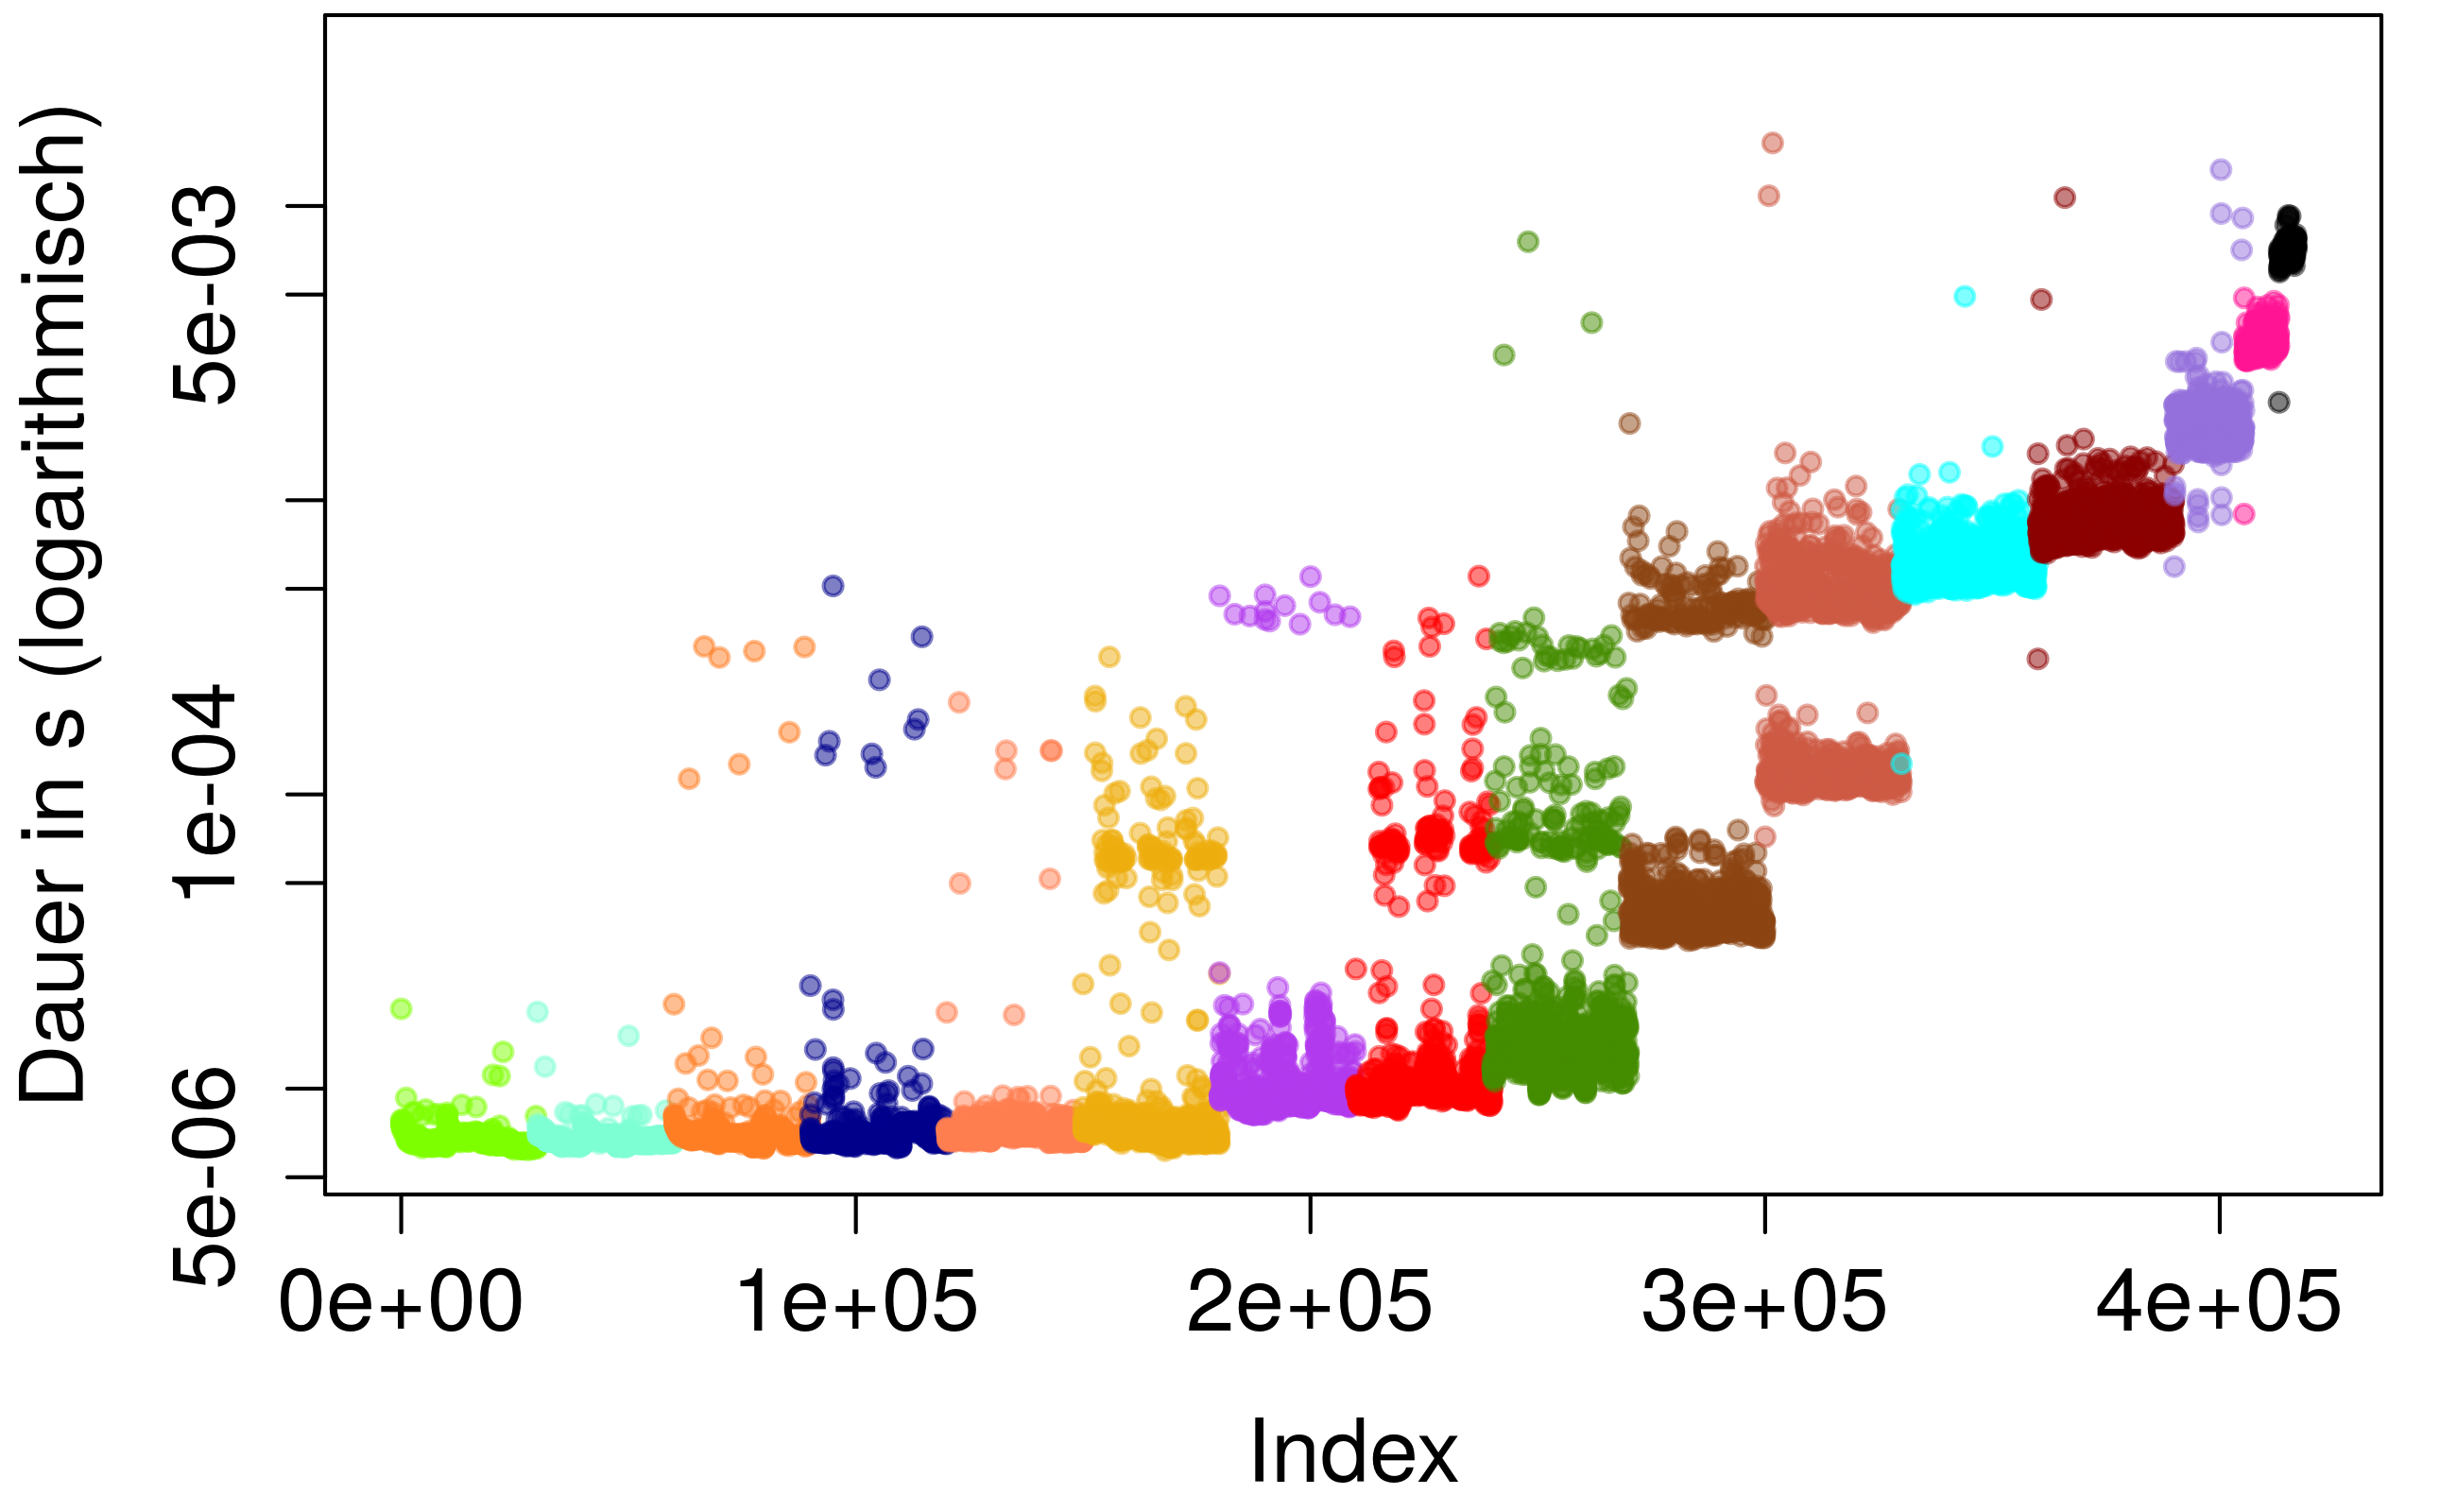
\includegraphics[width=.5\textwidth]{Bilder/Plots/exploration/plot_SizeSorted_log_read_seq.png}
	}
	\hfill
	\subfloat[Messungen in Zeitreihe zu SEQ-W]{
		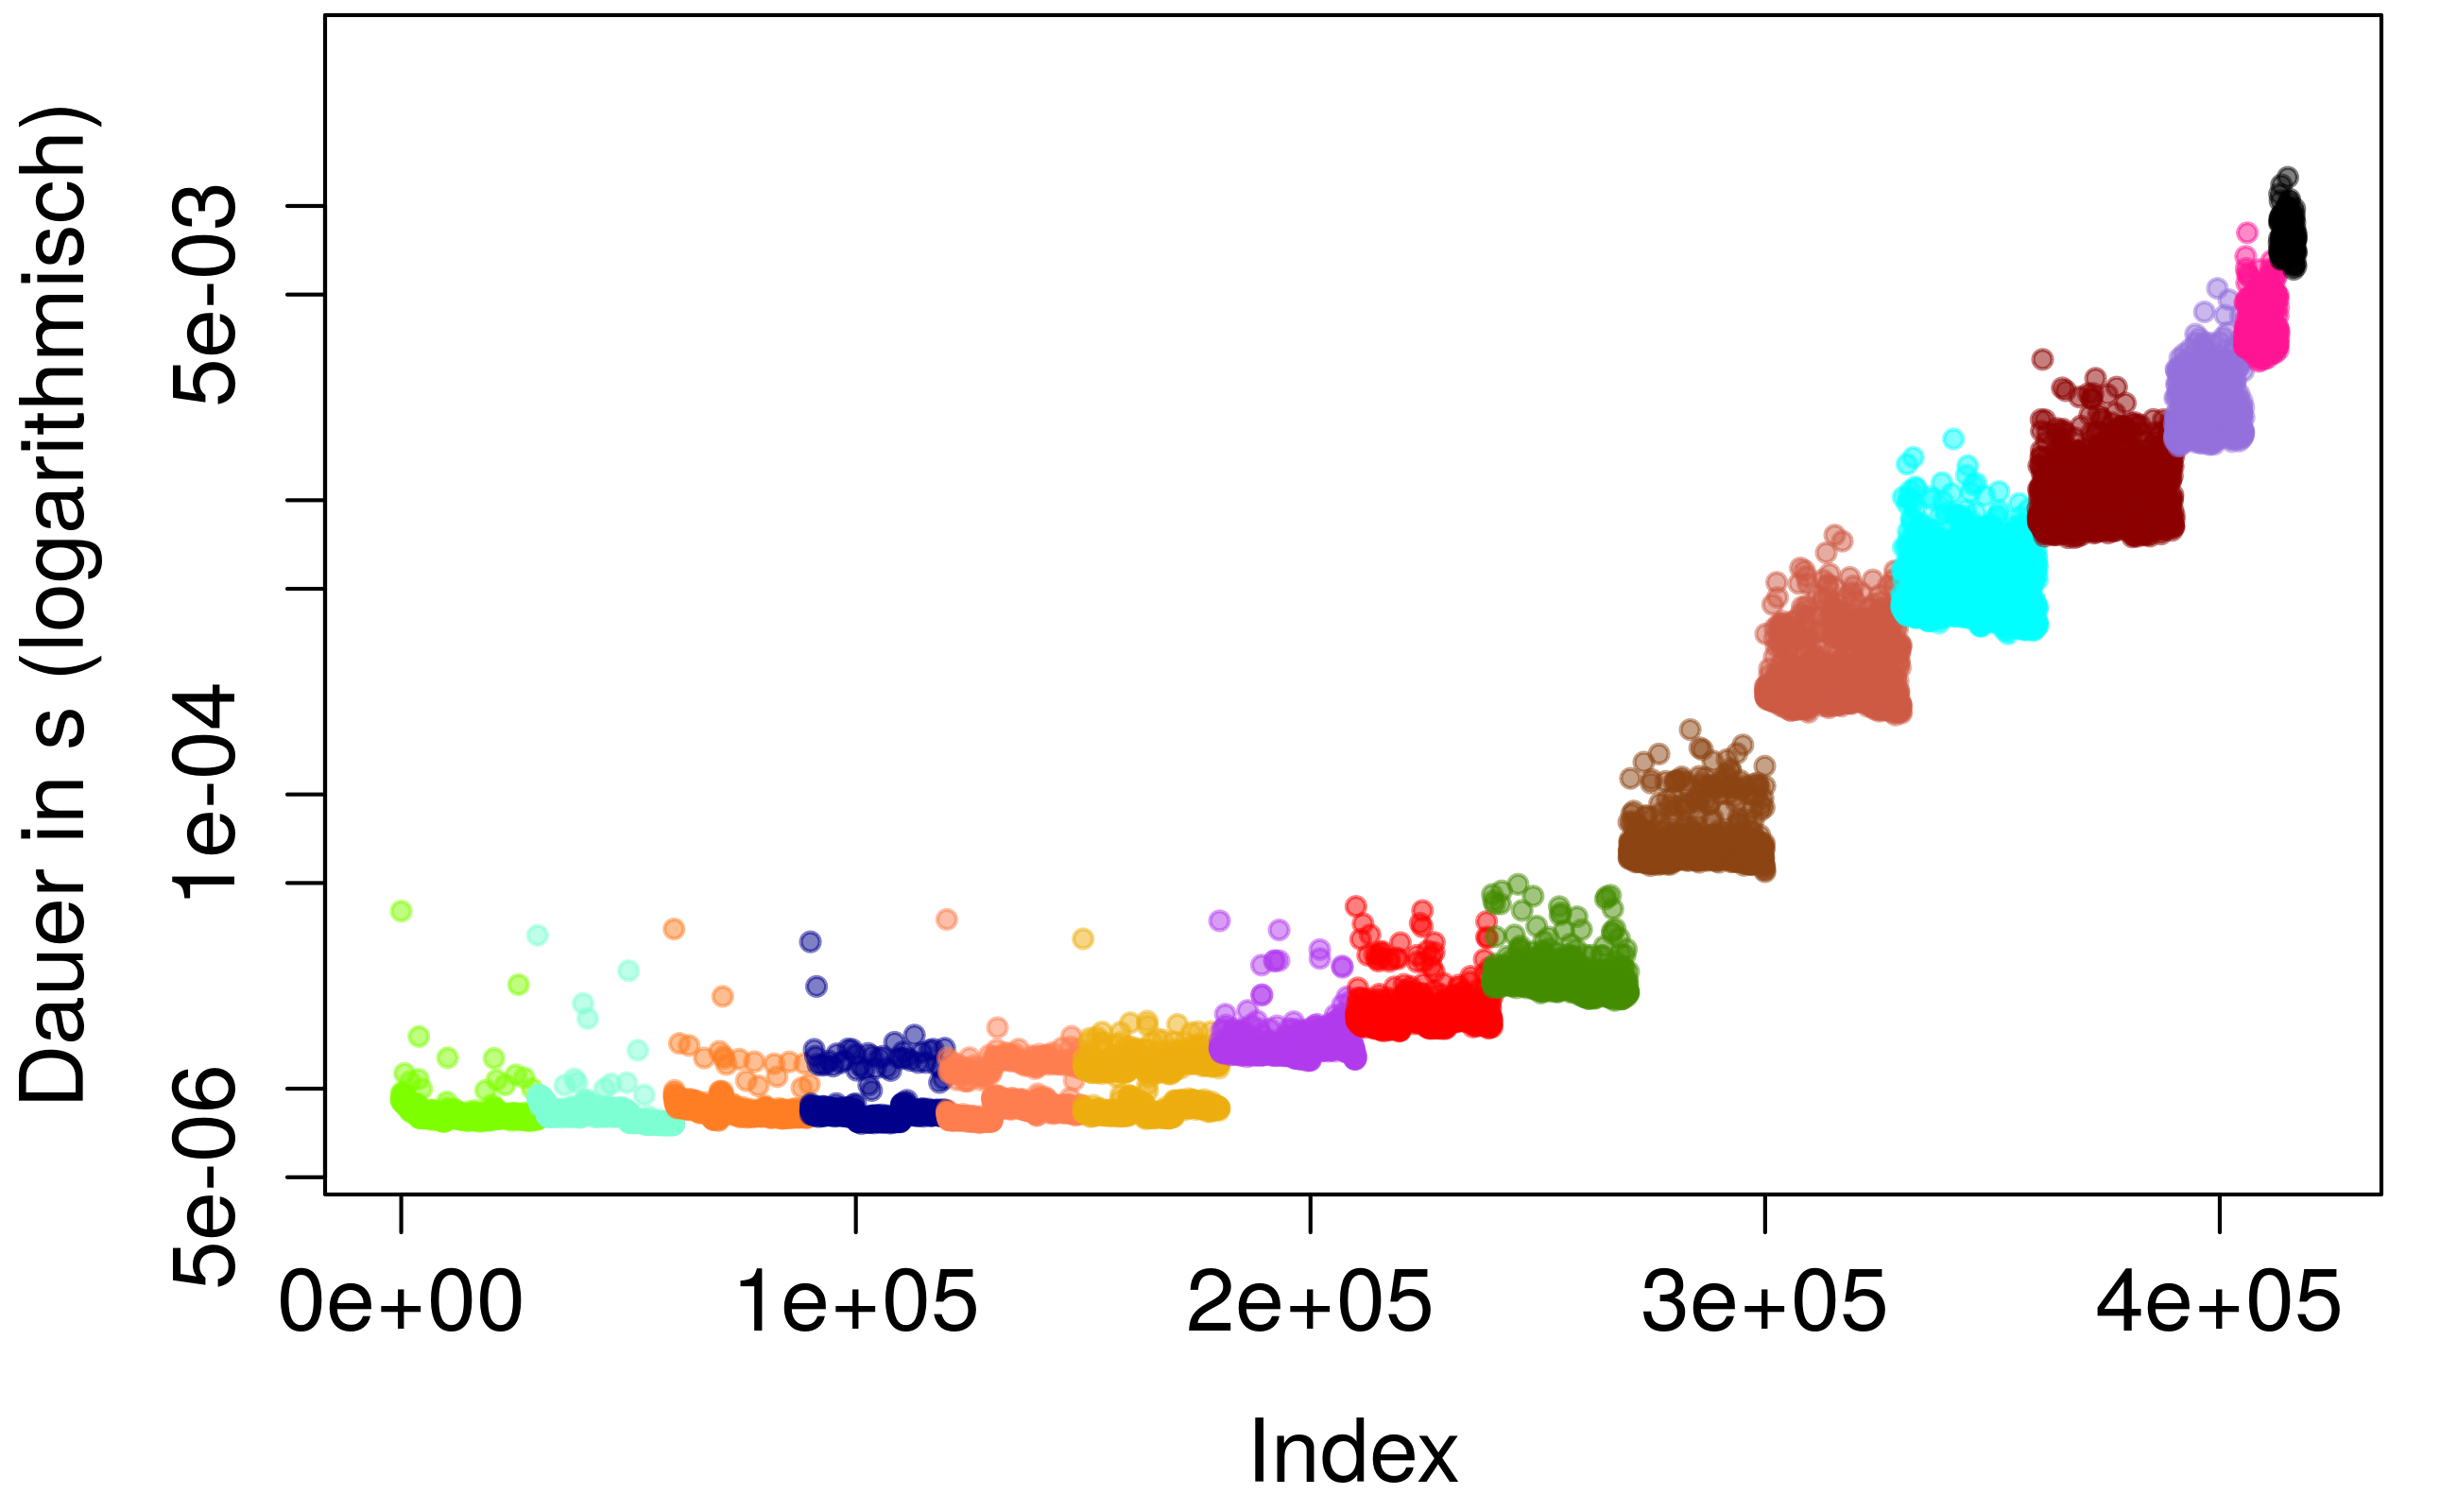
\includegraphics[width=.5\textwidth]{Bilder/Plots/exploration/plot_SizeSorted_log_write_seq.png}
	}\\
	\subfloat[Messungen in Zeitreihe zu RND-R]{
		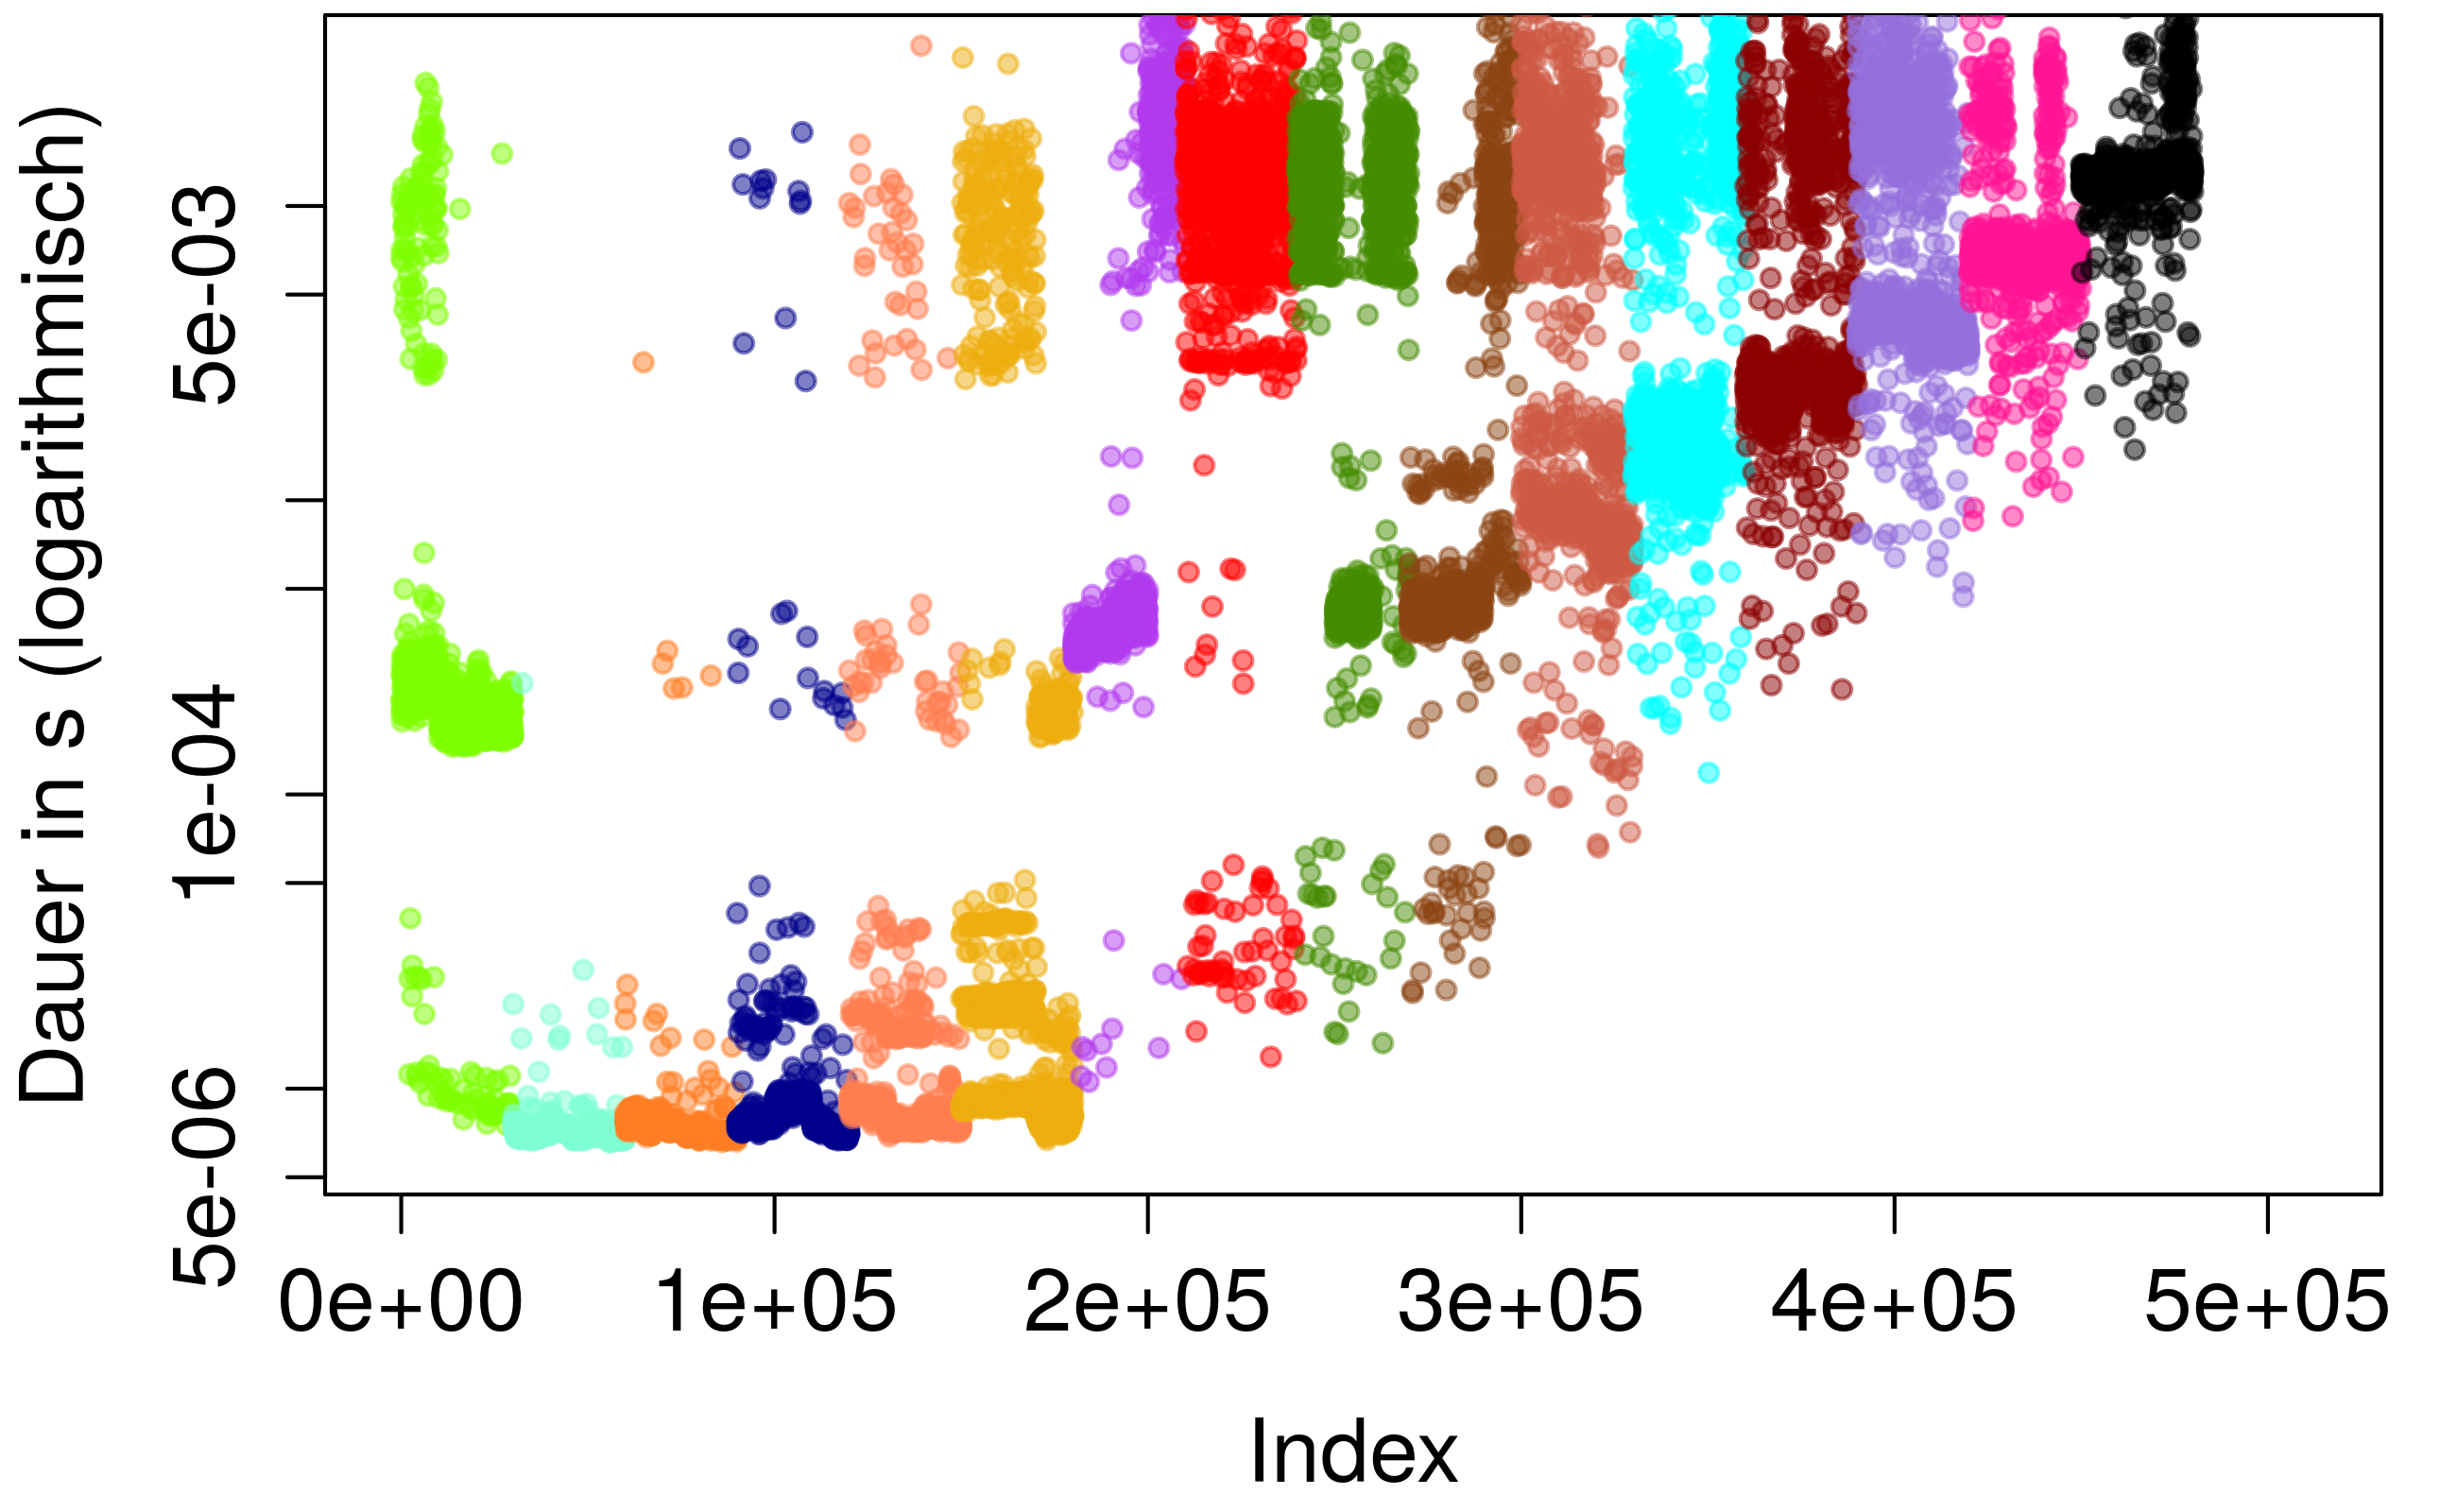
\includegraphics[width=.5\textwidth]{Bilder/Plots/exploration/plot_SizeSorted_log_read_rnd.png}
	}
	\hfill
	\subfloat[Messungen in Zeitreihe zu RND-W]{
		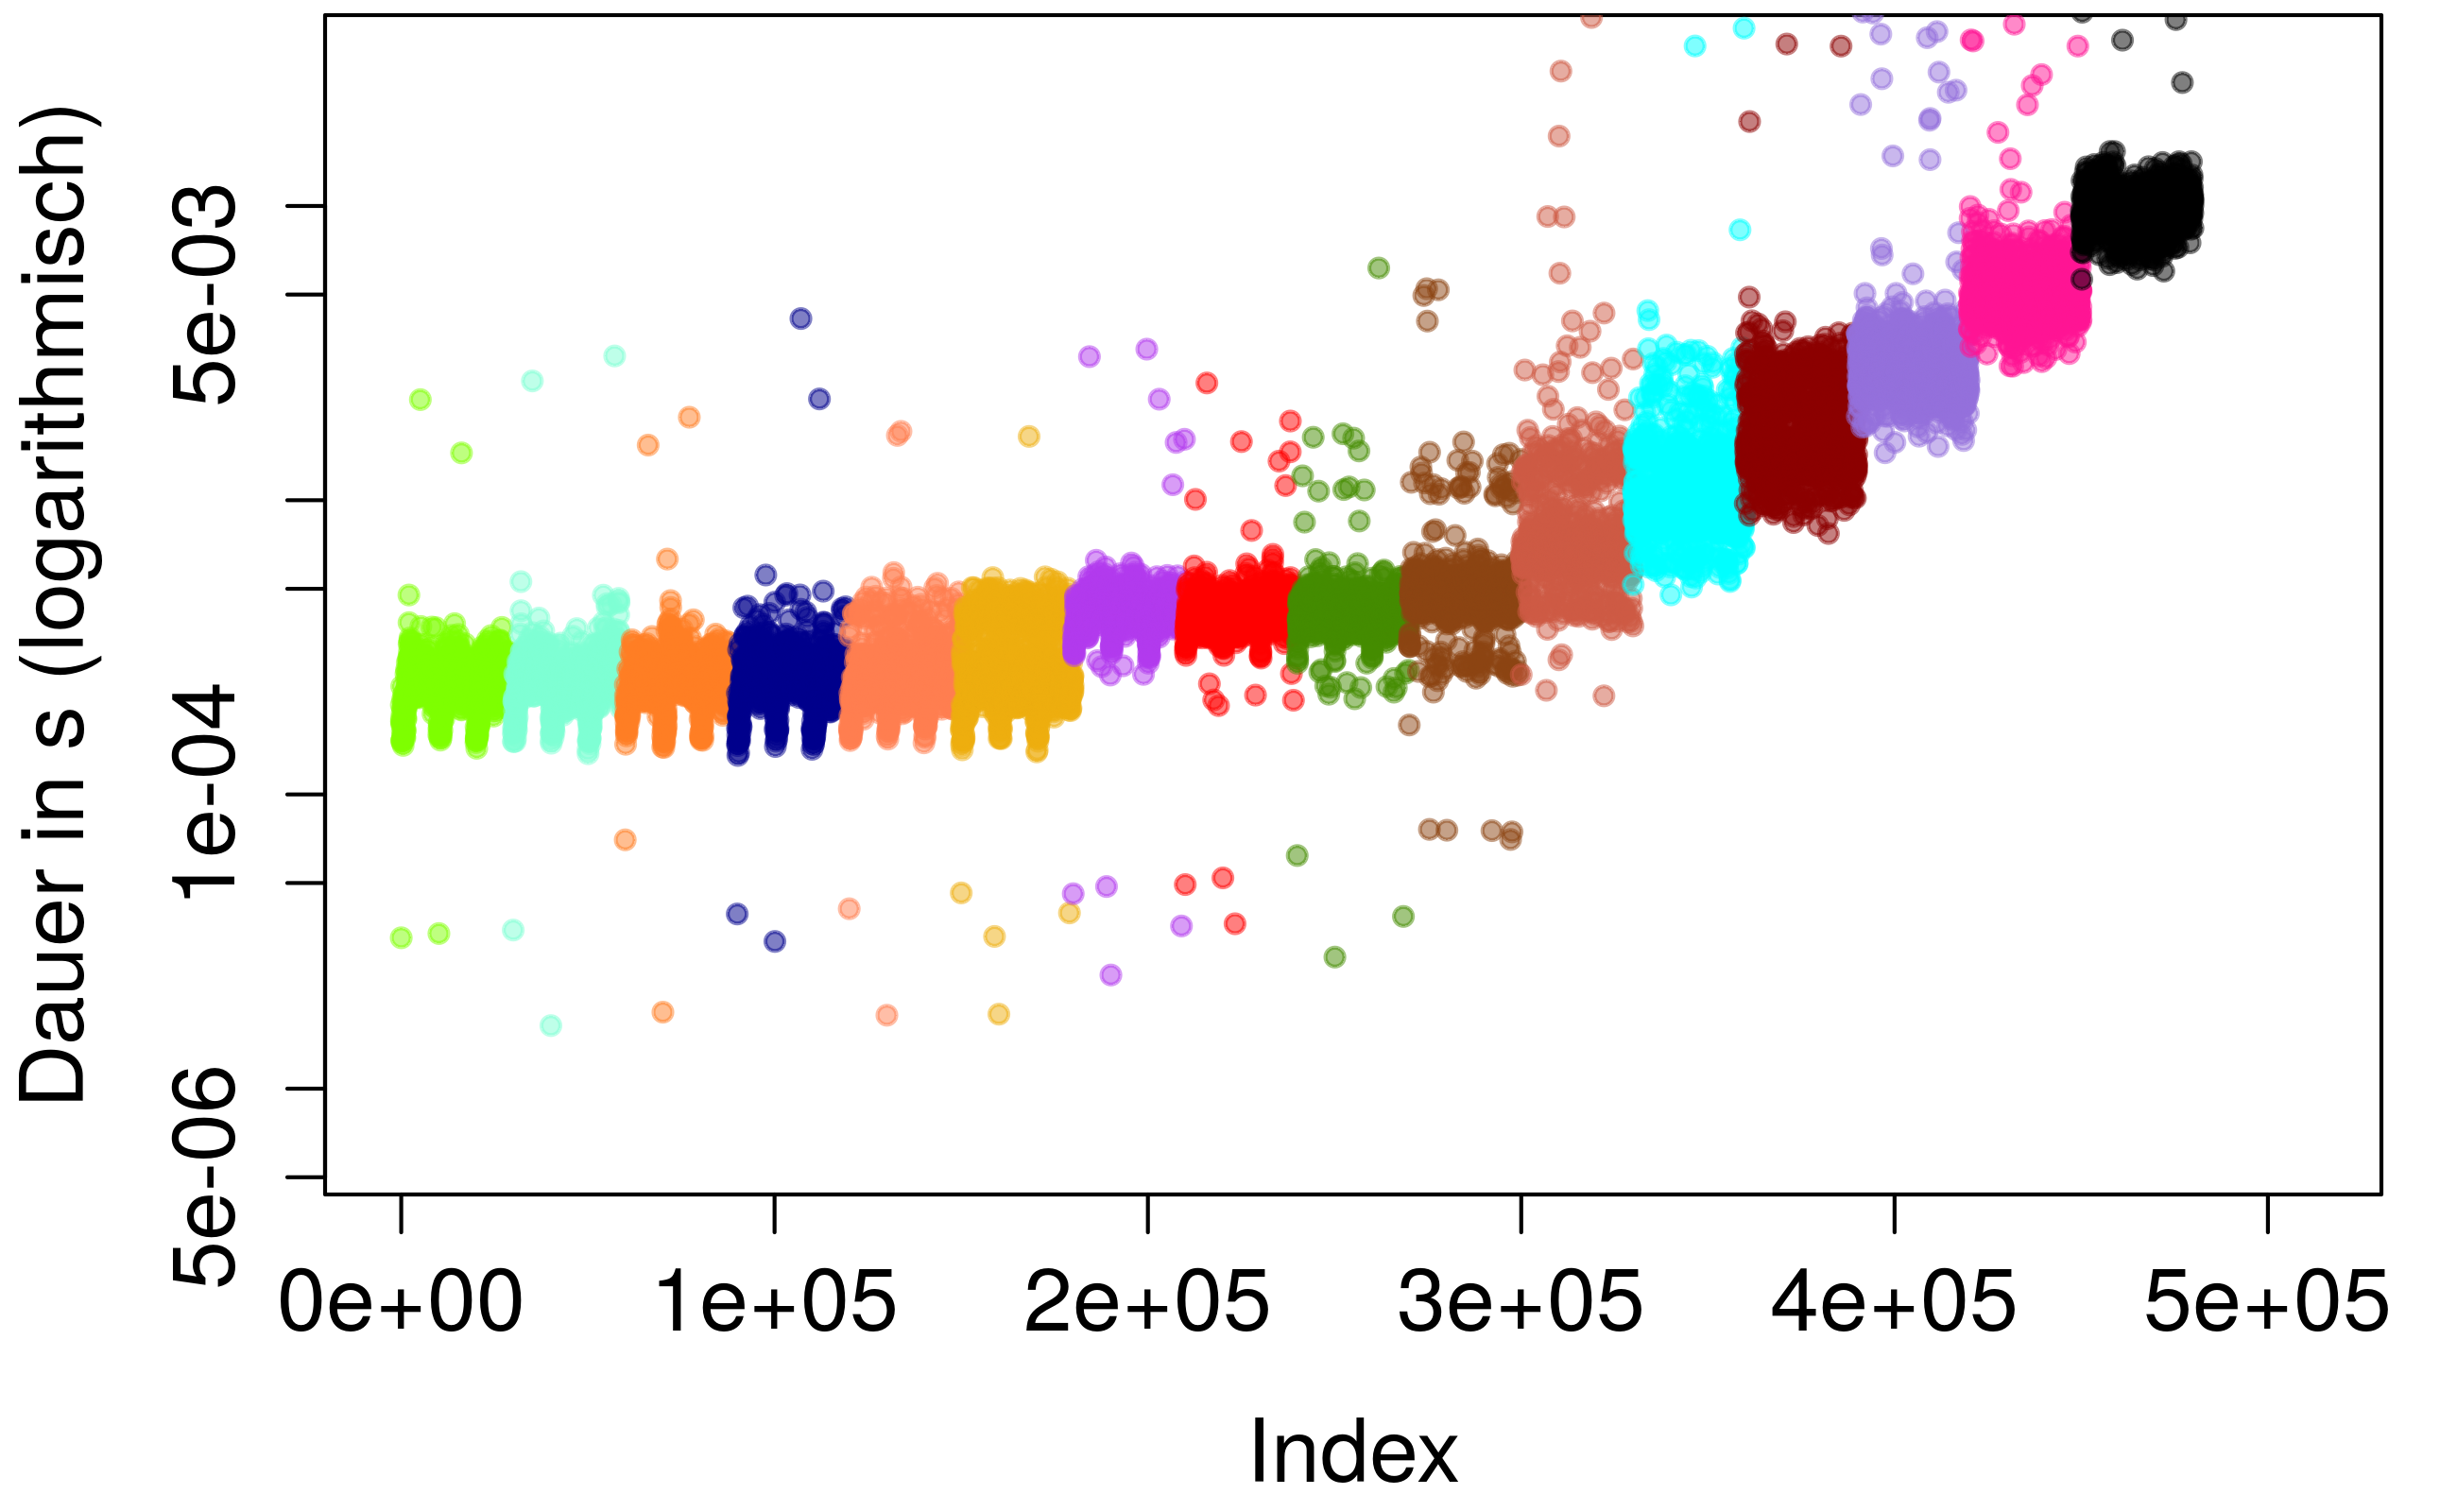
\includegraphics[width=.5\textwidth]{Bilder/Plots/exploration/plot_SizeSorted_log_write_rnd.png}
	}	
	\caption{Messungen der Laufzeiten nach Zugriffsgröße sortiert dargestellt. Von links nach rechts 1\,B, 4\,B, 16\,B, 64\,B, 256\,B, 1\,KiB, 4\,KiB, 8\,KiB, 16\,KiB, 64\,KiB, 256\,KiB, 512\,KiB, 1\,MiB, 2\,MiB, 4\,MiB, 8\,MiB und 16\,MiB}
	\label{Laufzeiten_Zeitreihe}
\end{figure} 

\subsubsection{Verteilung der Zugriffszeiten}
Der in Abschnitt \ref{analyse:ea_pfad_zurvorhersage} beschriebene Zusammenhang zwischen E/A-Pfad und Zugriffszeit wurde anhand von Abbildung \ref{Laufzeiten_Zeitreihe}a verdeutlicht.
Für RND-R ergeben sich ähnliche Beobachtungen, während die Abhängigkeit zwischen E/A-Pfad und Laufzeit bei den beiden Abbildungen zu Messreihen mit zufälligen Dateizugriffen weniger deutlich zu sein scheint. Aber auch hier lässt sich teilweise eine Aufspaltung der Messungen mit gleicher Zugriffsgröße in zwei Gruppen beobachten.\medskip

Wenn die Messpunkte nach der Laufzeit sortiert werden (siehe Abbildung \ref{Laufzeiten_Sortiert}), können die verschiedenen Stufen der Laufzeiten besser betrachtet werden.
Bestimmte Laufzeiten kommen häufiger vor, sie kennzeichnen sich als Auftritt der Stufen. Andere Laufzeiten kommen dagegen seltener vor, sie bilden eine Senkrechte.
Die Stufen entstehen einerseits durch die Messung unterschiedlicher Zugriffsgrößen (mit größeren Abständen zwischen verschiedenen Größen), teilweise lassen sie sich aber auch als die beschriebenen E/A-Pfade im System interpretieren.\medskip

Die geringe Aufteilung der Messungen in Gruppen bei den beiden Datensätzen zu schreibenden E/A-Aufrufen sprechen dafür, dass die Stufen durch die Messung verschiedener Zugriffsgrößen entstanden sind.
Der andere Fall lässt sich besonders gut bei RND-R erkennen. Die Zugriffszeiten zu einer Größe teilen sich in Abbildung \ref{Laufzeiten_Zeitreihe}c in etwa drei Gruppen auf, eine langsame, eine mittlere und eine schnelle.
Die Gruppen verschiedener Zugriffsgrößen können teilweise zu einem E/A-Pfad zusammengefasst werden. Die Häufungen finden sich dann auf einer horizontalen Linie. 
Die Laufzeit ist für die horizontal nebeneinanderliegenden Gruppen nicht vorwiegend von der Zugriffsgröße abhängig, sondern in unserer Interpretation von dem Pfad, den die entsprechenden Aufrufe im System genommen haben. 

\begin{figure}
	\centering
	\subfloat[SEQ-R]{
		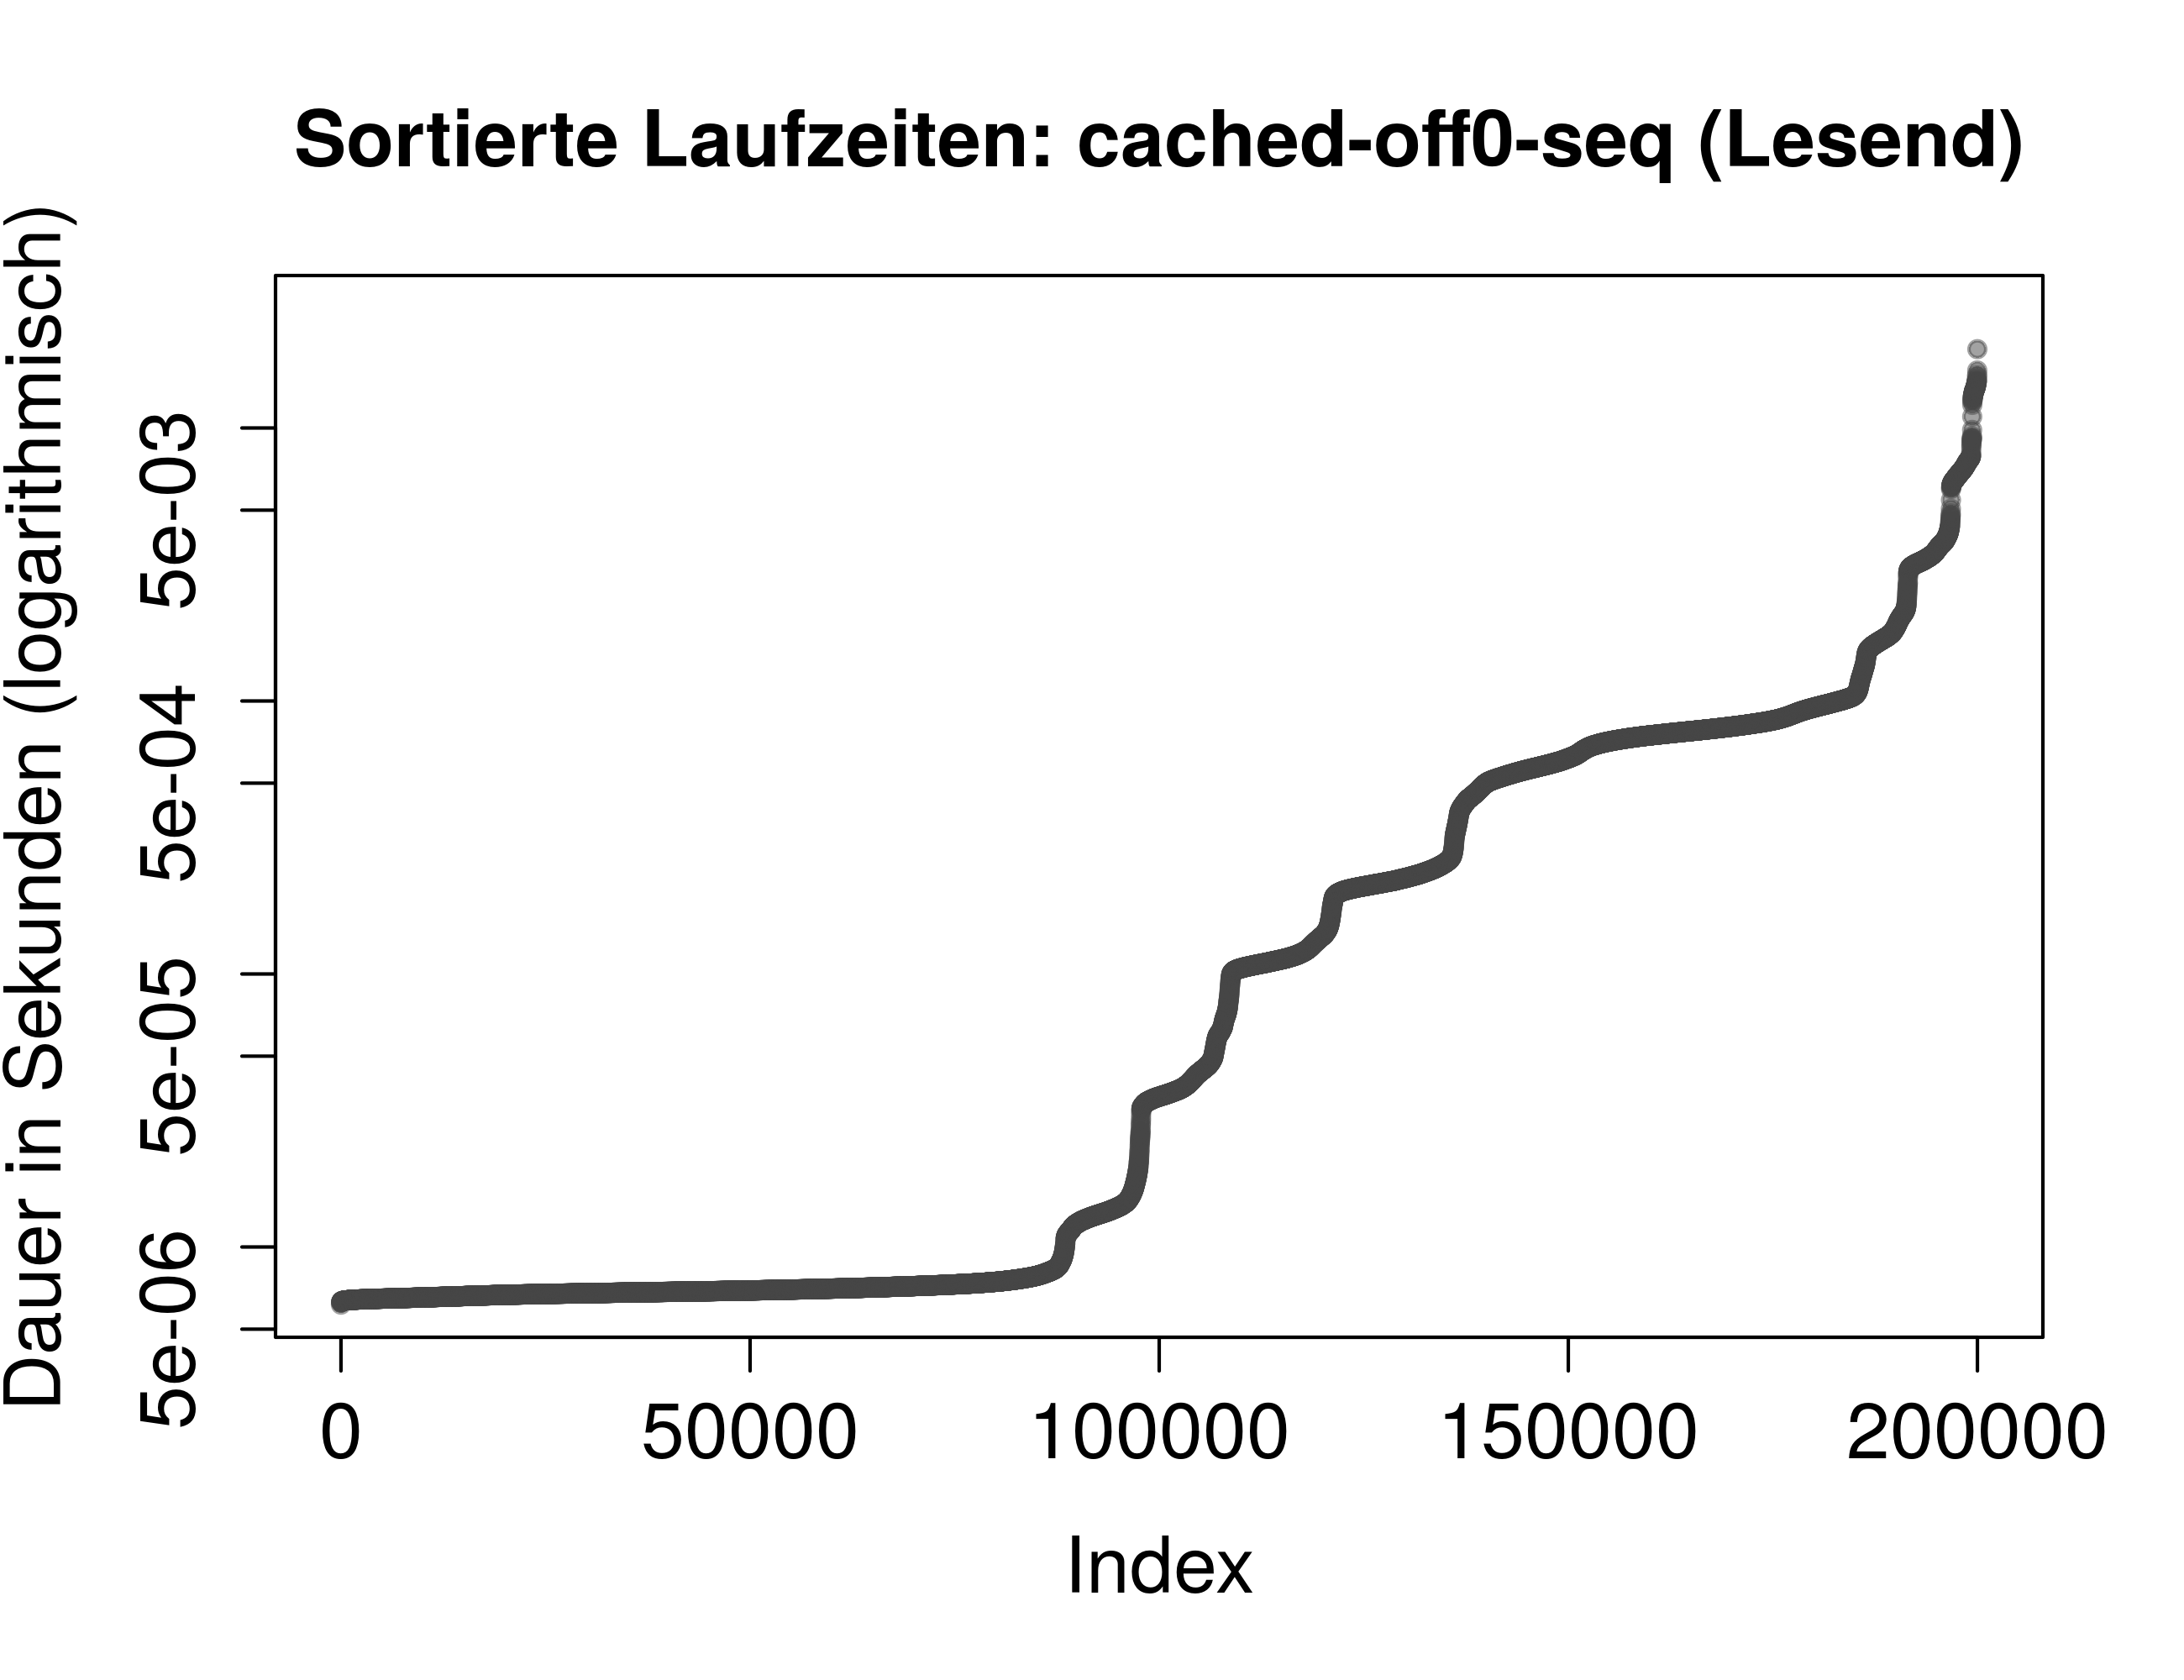
\includegraphics[width=.46\textwidth]{Bilder/Plots/exploration/plot_DurationSorted_read_seq.png}
	}
	\hfill
	\subfloat[SEQ-W]{
		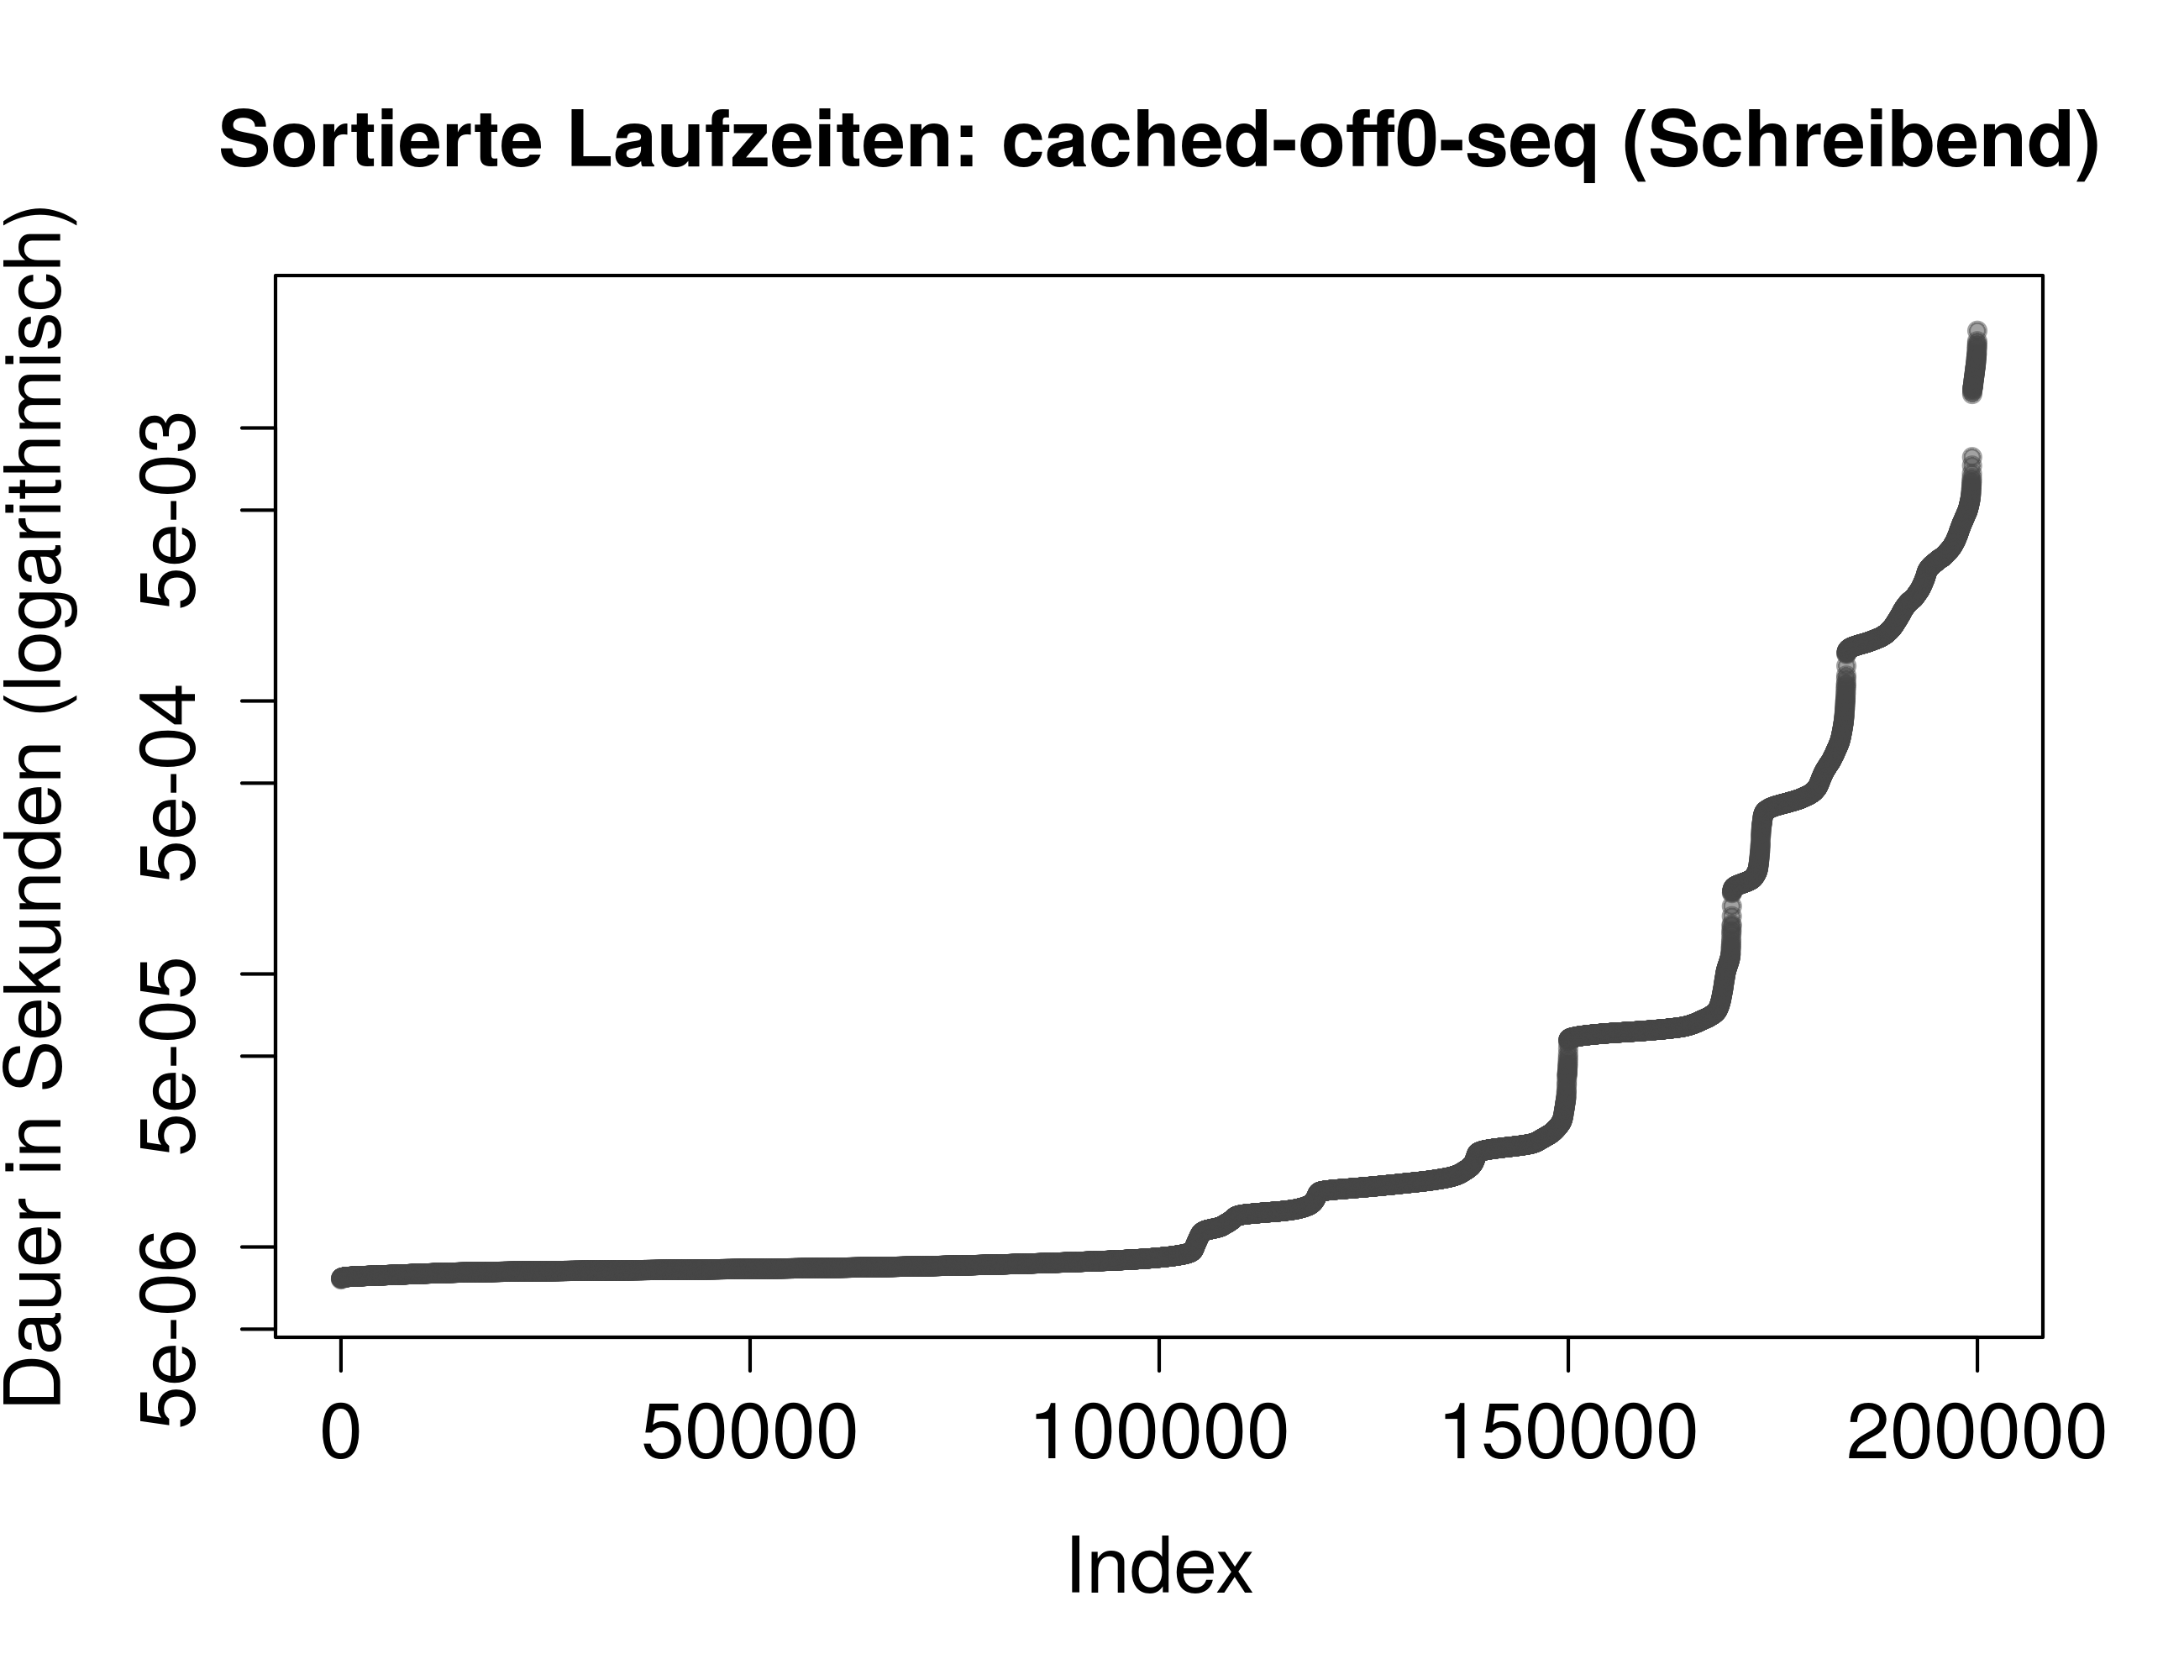
\includegraphics[width=.46\textwidth]{Bilder/Plots/exploration/plot_DurationSorted_write_seq.png}
	}\\
	\subfloat[RND-R]{
		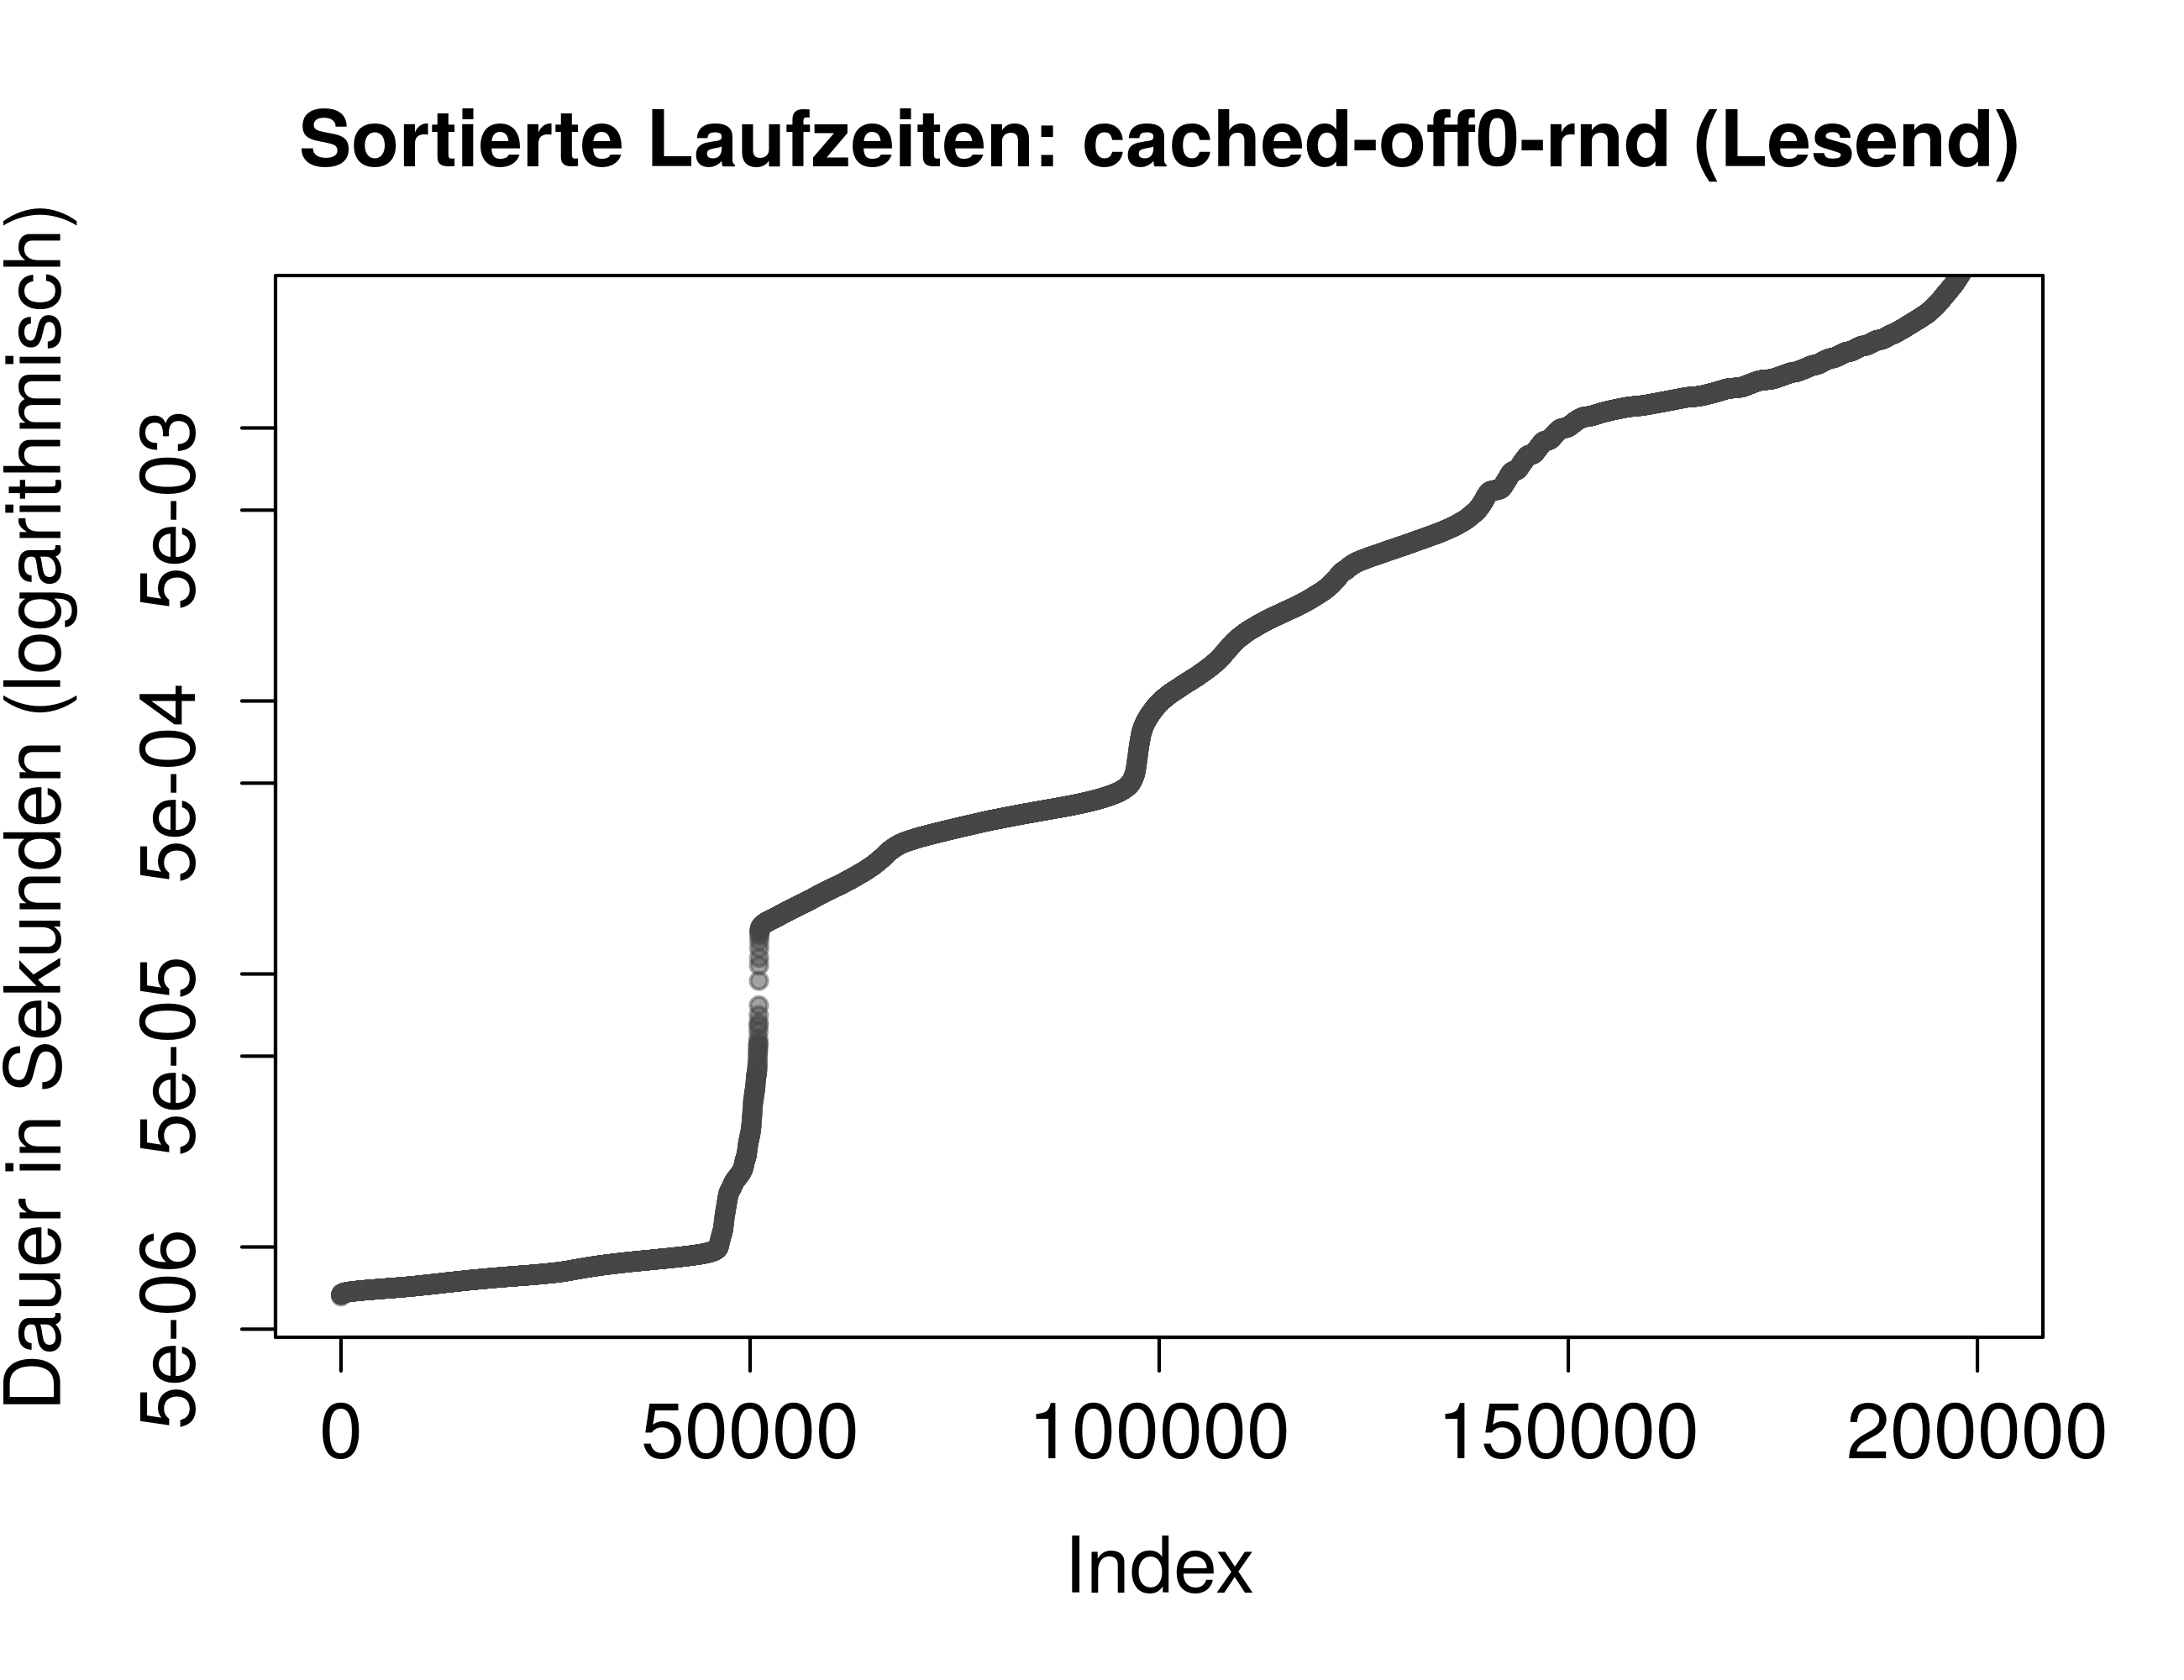
\includegraphics[width=.46\textwidth]{Bilder/Plots/exploration/plot_DurationSorted_read_rnd.png}
	}
	\hfill
	\subfloat[RND-W]{
		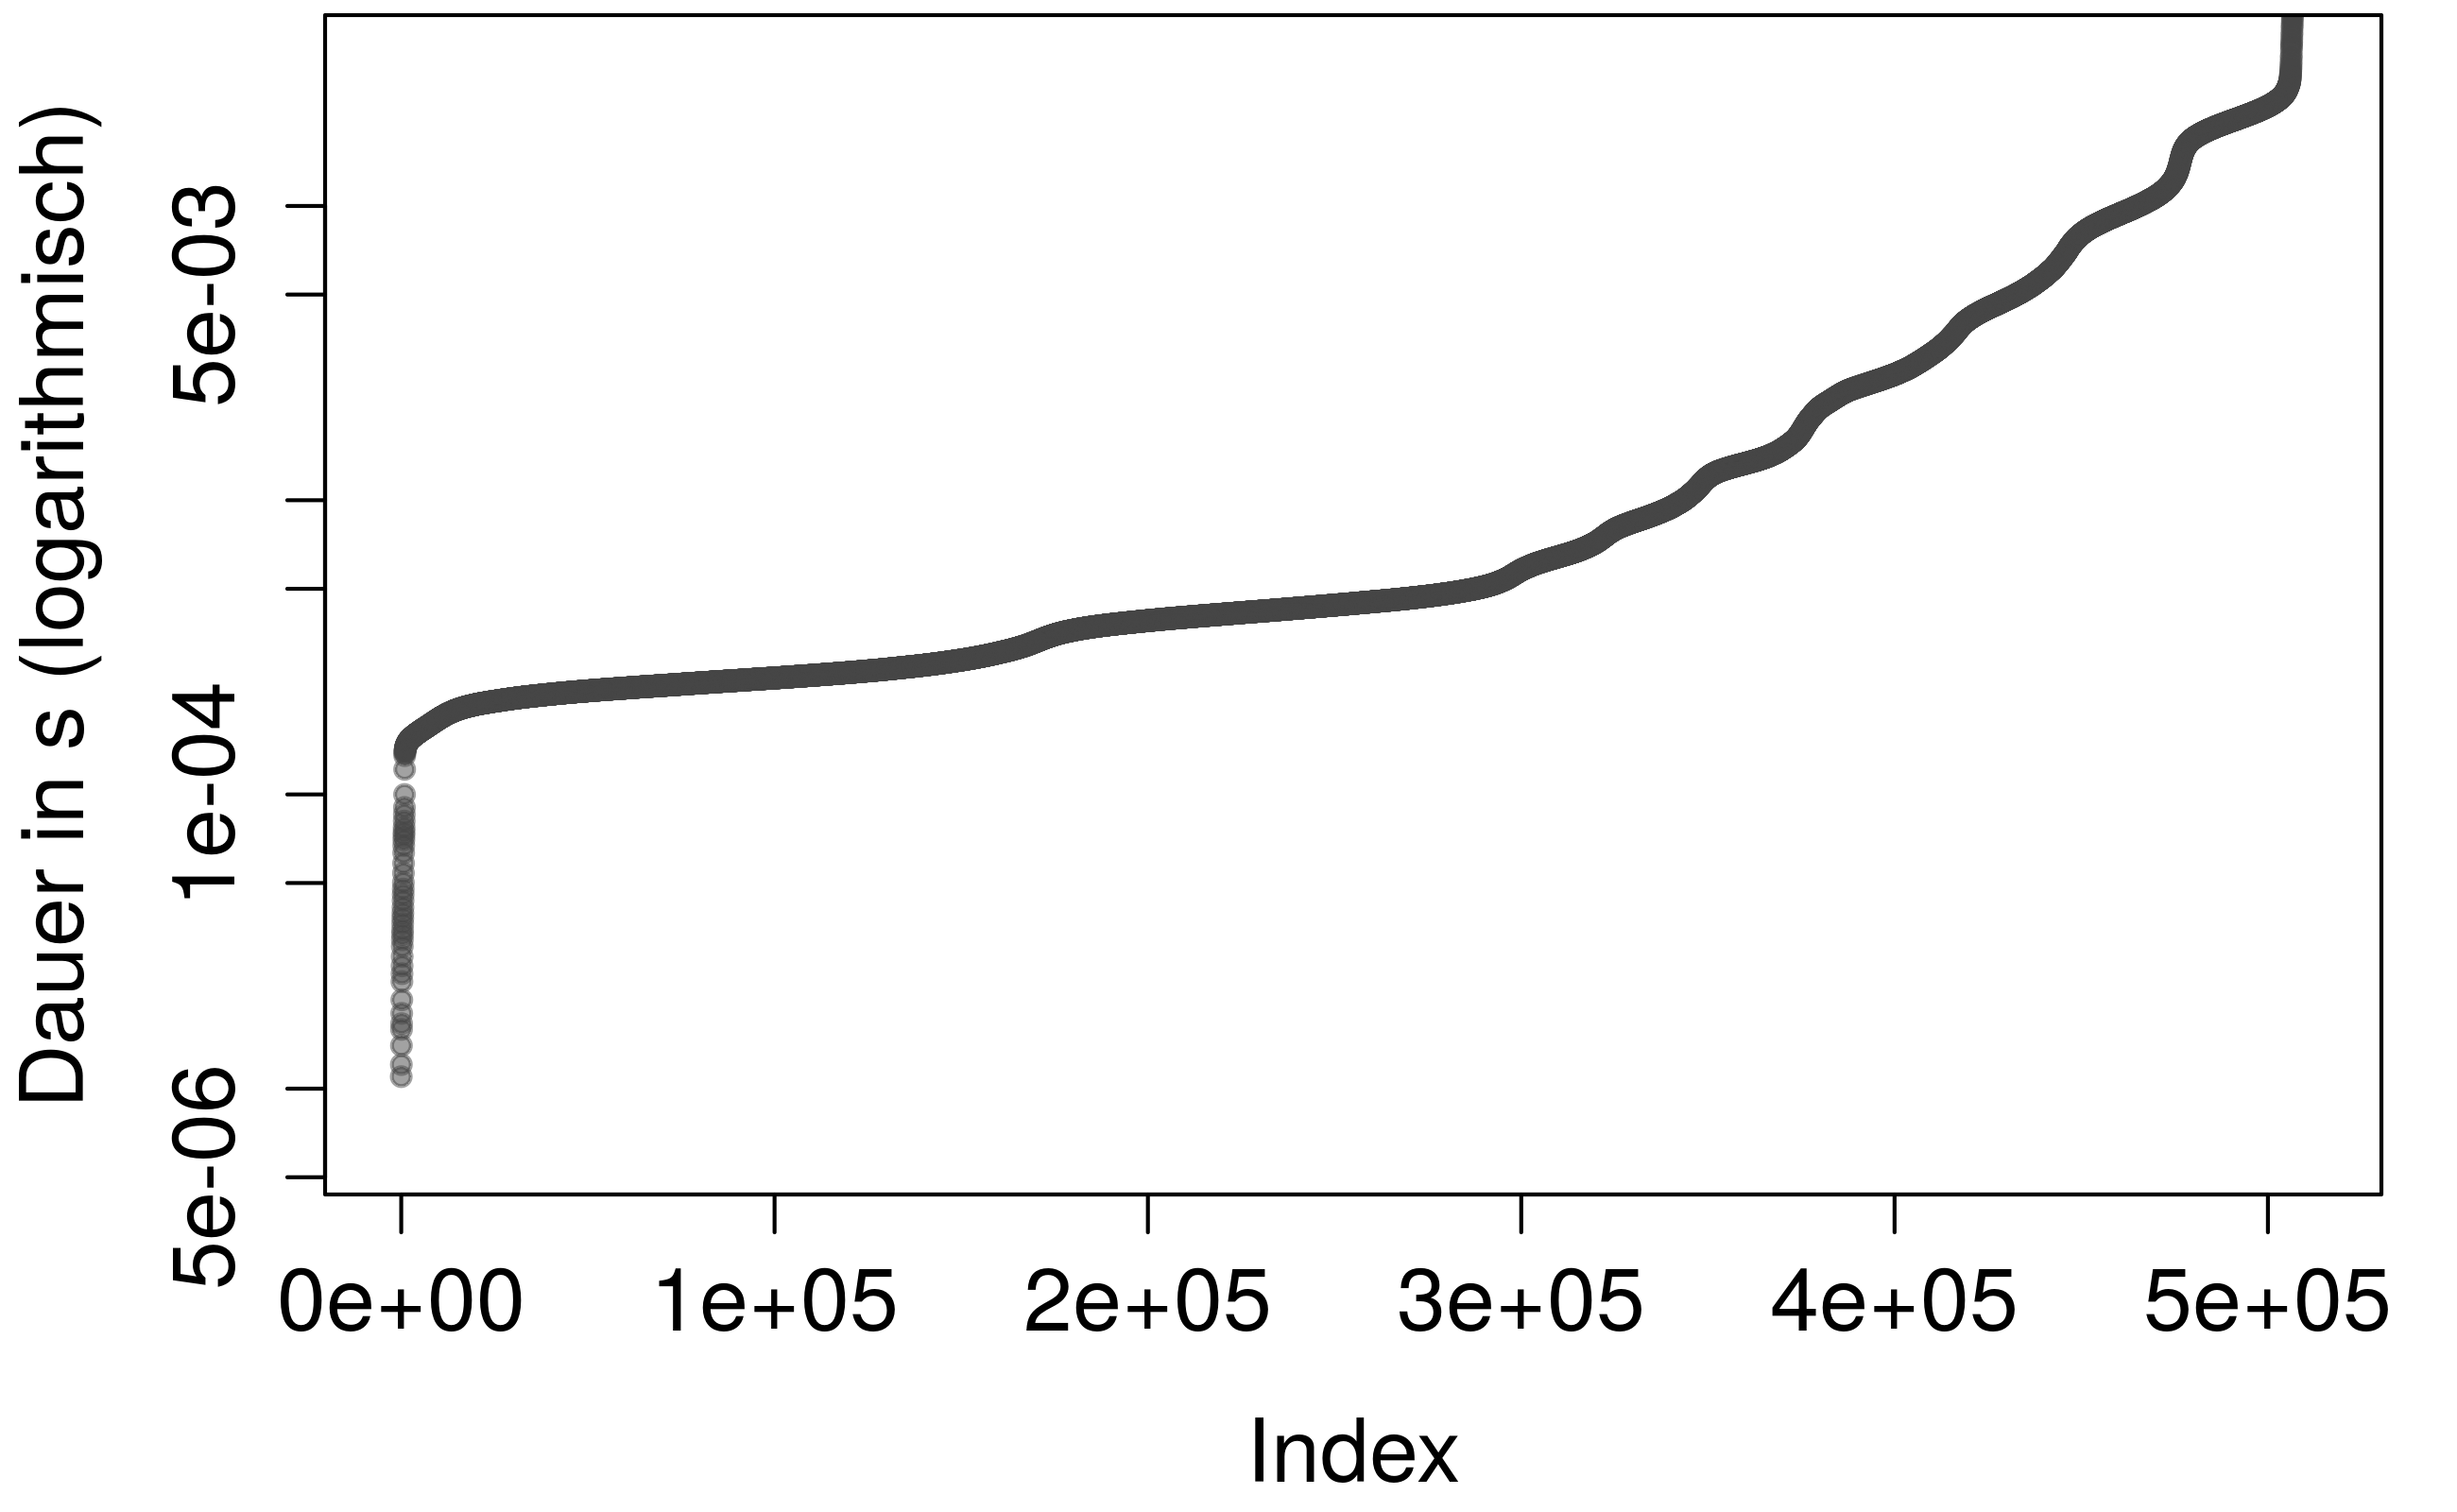
\includegraphics[width=.46\textwidth]{Bilder/Plots/exploration/plot_DurationSorted_write_rnd.png}
	}		
	\caption{Messungen der Laufzeiten sortiert dargestellt.}
	\label{Laufzeiten_Sortiert}
\end{figure} 

\subsubsection{Betrachtung der Ausreißer}
Als Ausreißer werden für alle Attribut-Tupel die Messungen mit den $10\%$ kürzesten und längsten Laufzeiten behandelt. Die Verteilung der Ausreißer ist in Abbildung \ref{fig:ausreisser} zu erkennen.
Bei den randomisierten Messungen gibt es pro Attribut-Tupel nur ein bis drei Messungen. Eine Ausreißerbetrachtung, wie sie hier gemacht wird, macht auf den entsprechenden Datensätzen keinen Sinn. Die Stichprobe zu den verschiedenen Attribut-Tupel ist dafür zu klein.
Die Ausreißervorhersage wird dementsprechend im Folgenden nur auf dem sequentiellen Datensatz durchgeführt.
In Abbildung \ref{fig:ausreisser} sind die Ausreißer rot markiert, sie befinden sich gerade an den oberen und unteren Enden einer Stufe.

\begin{figure}
	\centering
	\subfloat[SEQ-R]{
		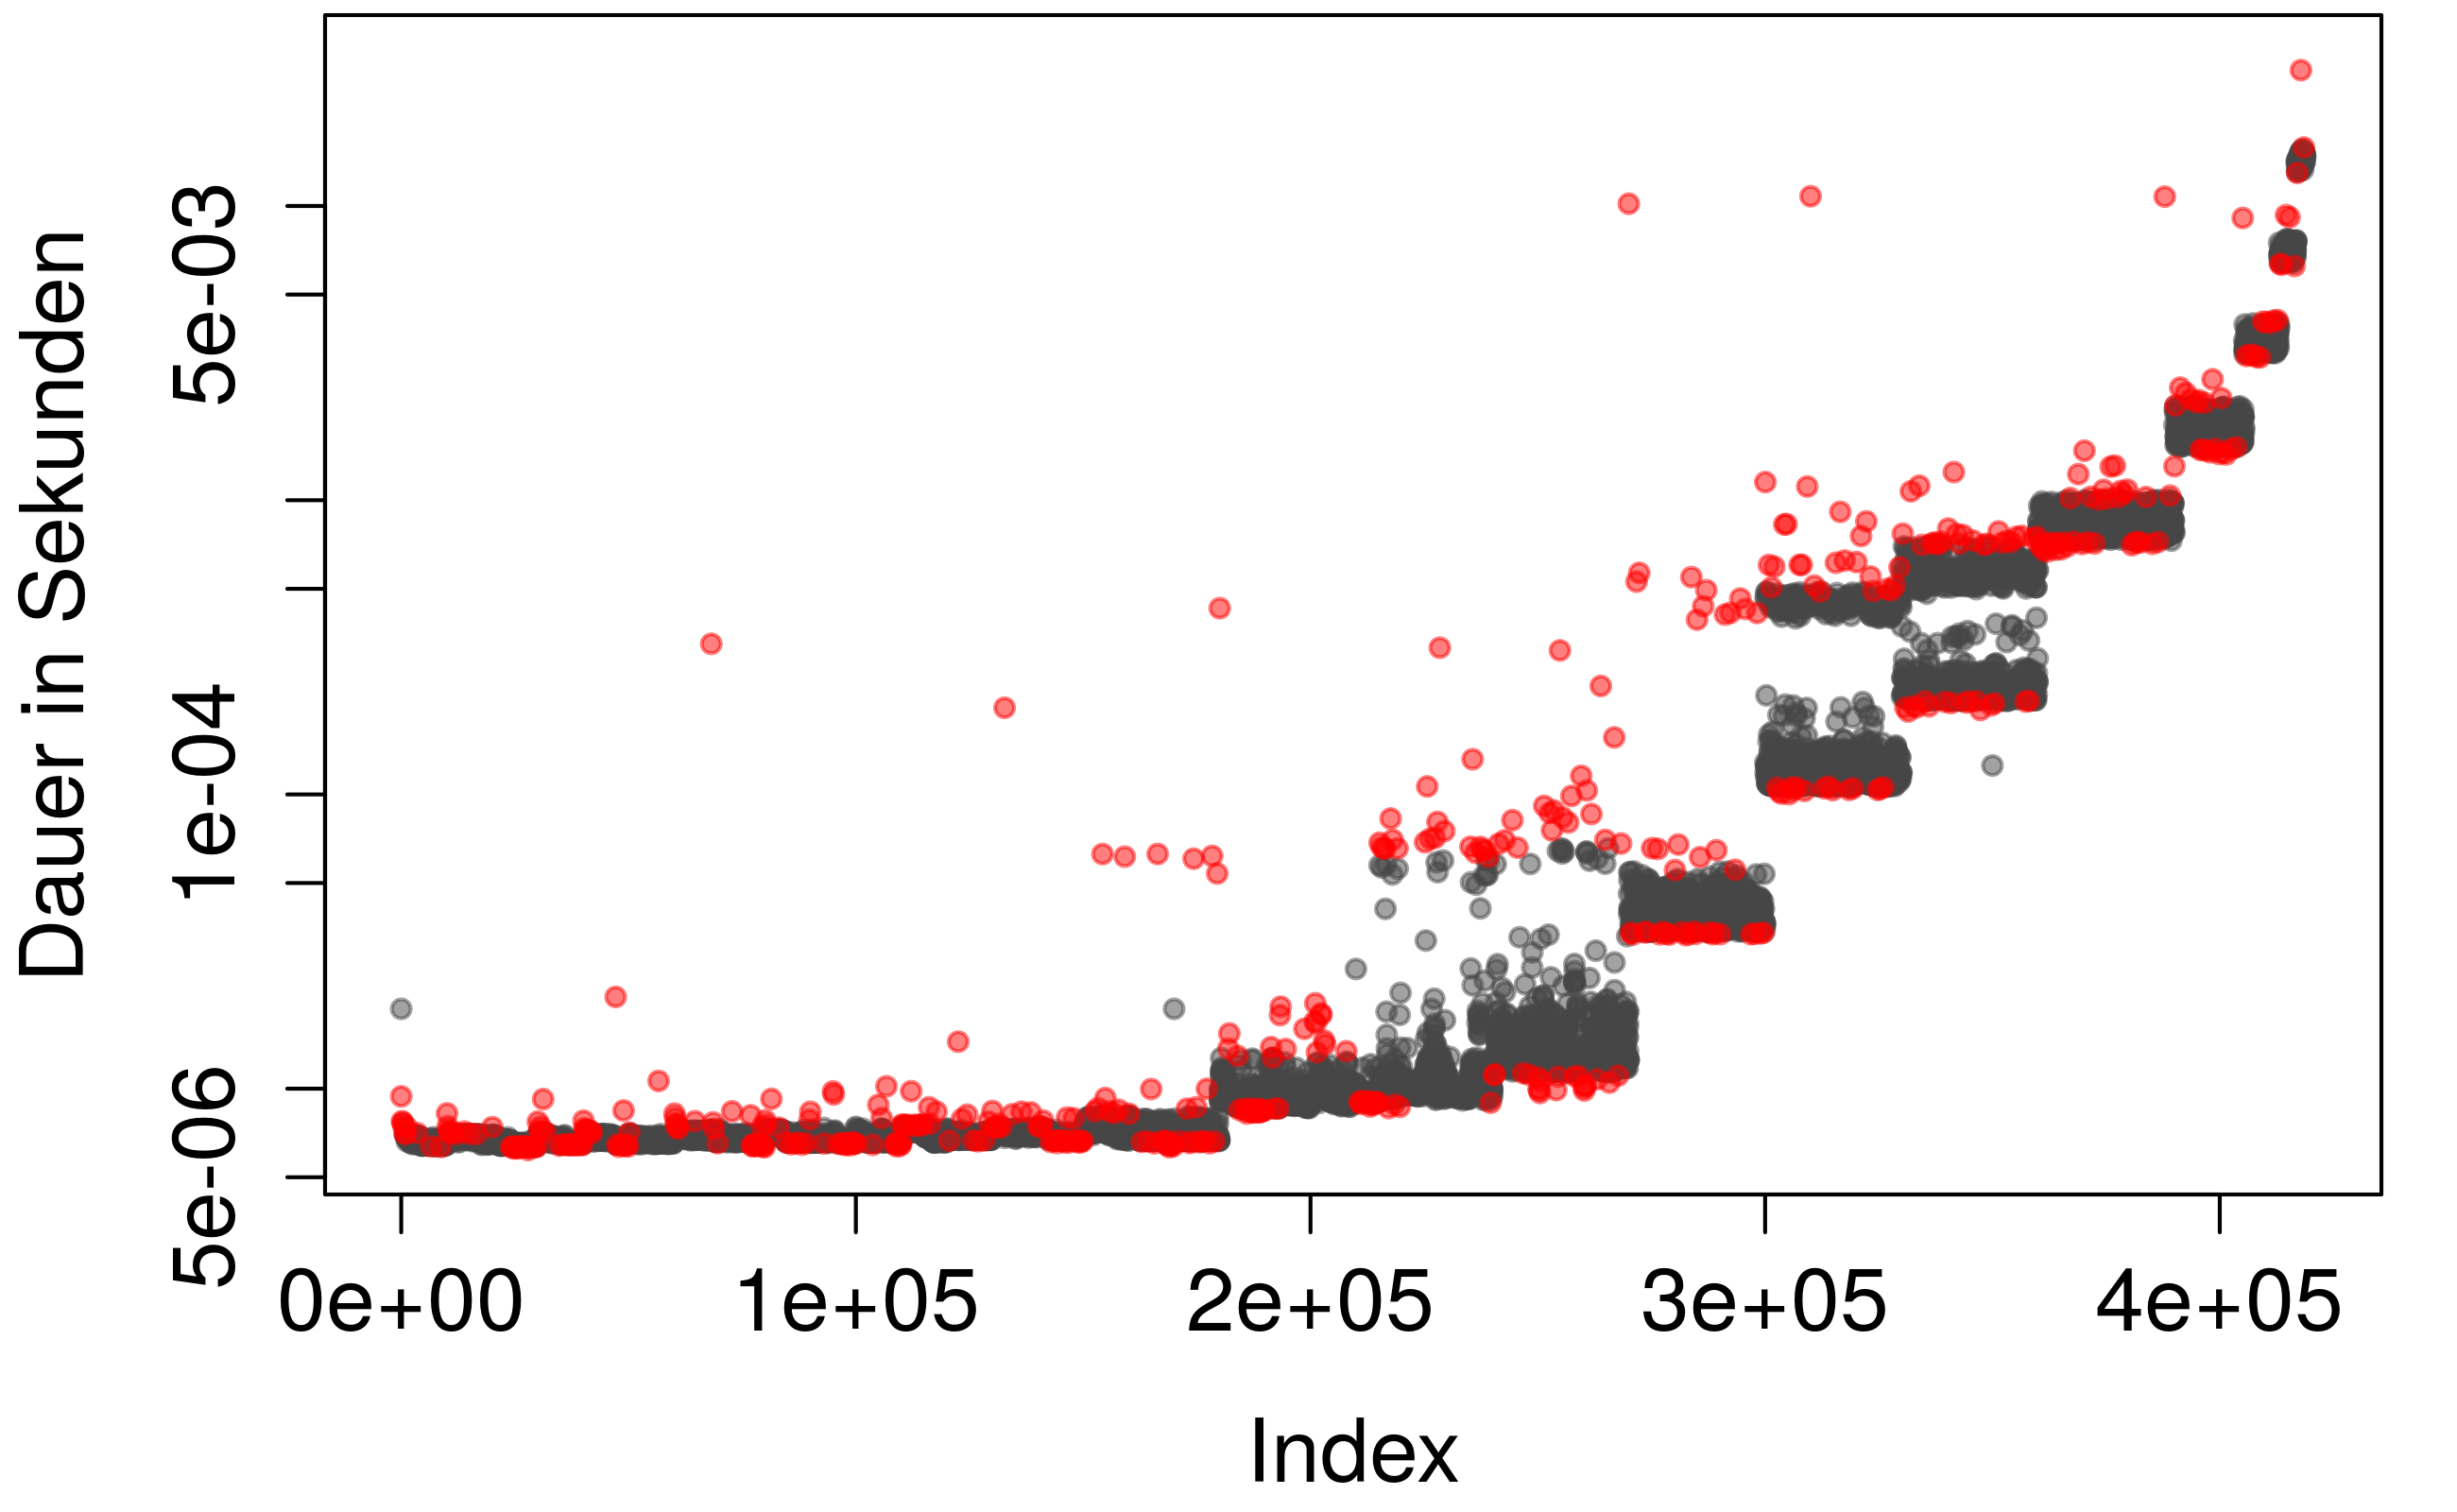
\includegraphics[width=.46\textwidth]{Bilder/Plots/exploration/plot_outlier_read_seq.png}
	}
	\hfill
	\subfloat[SEQ-W]{
		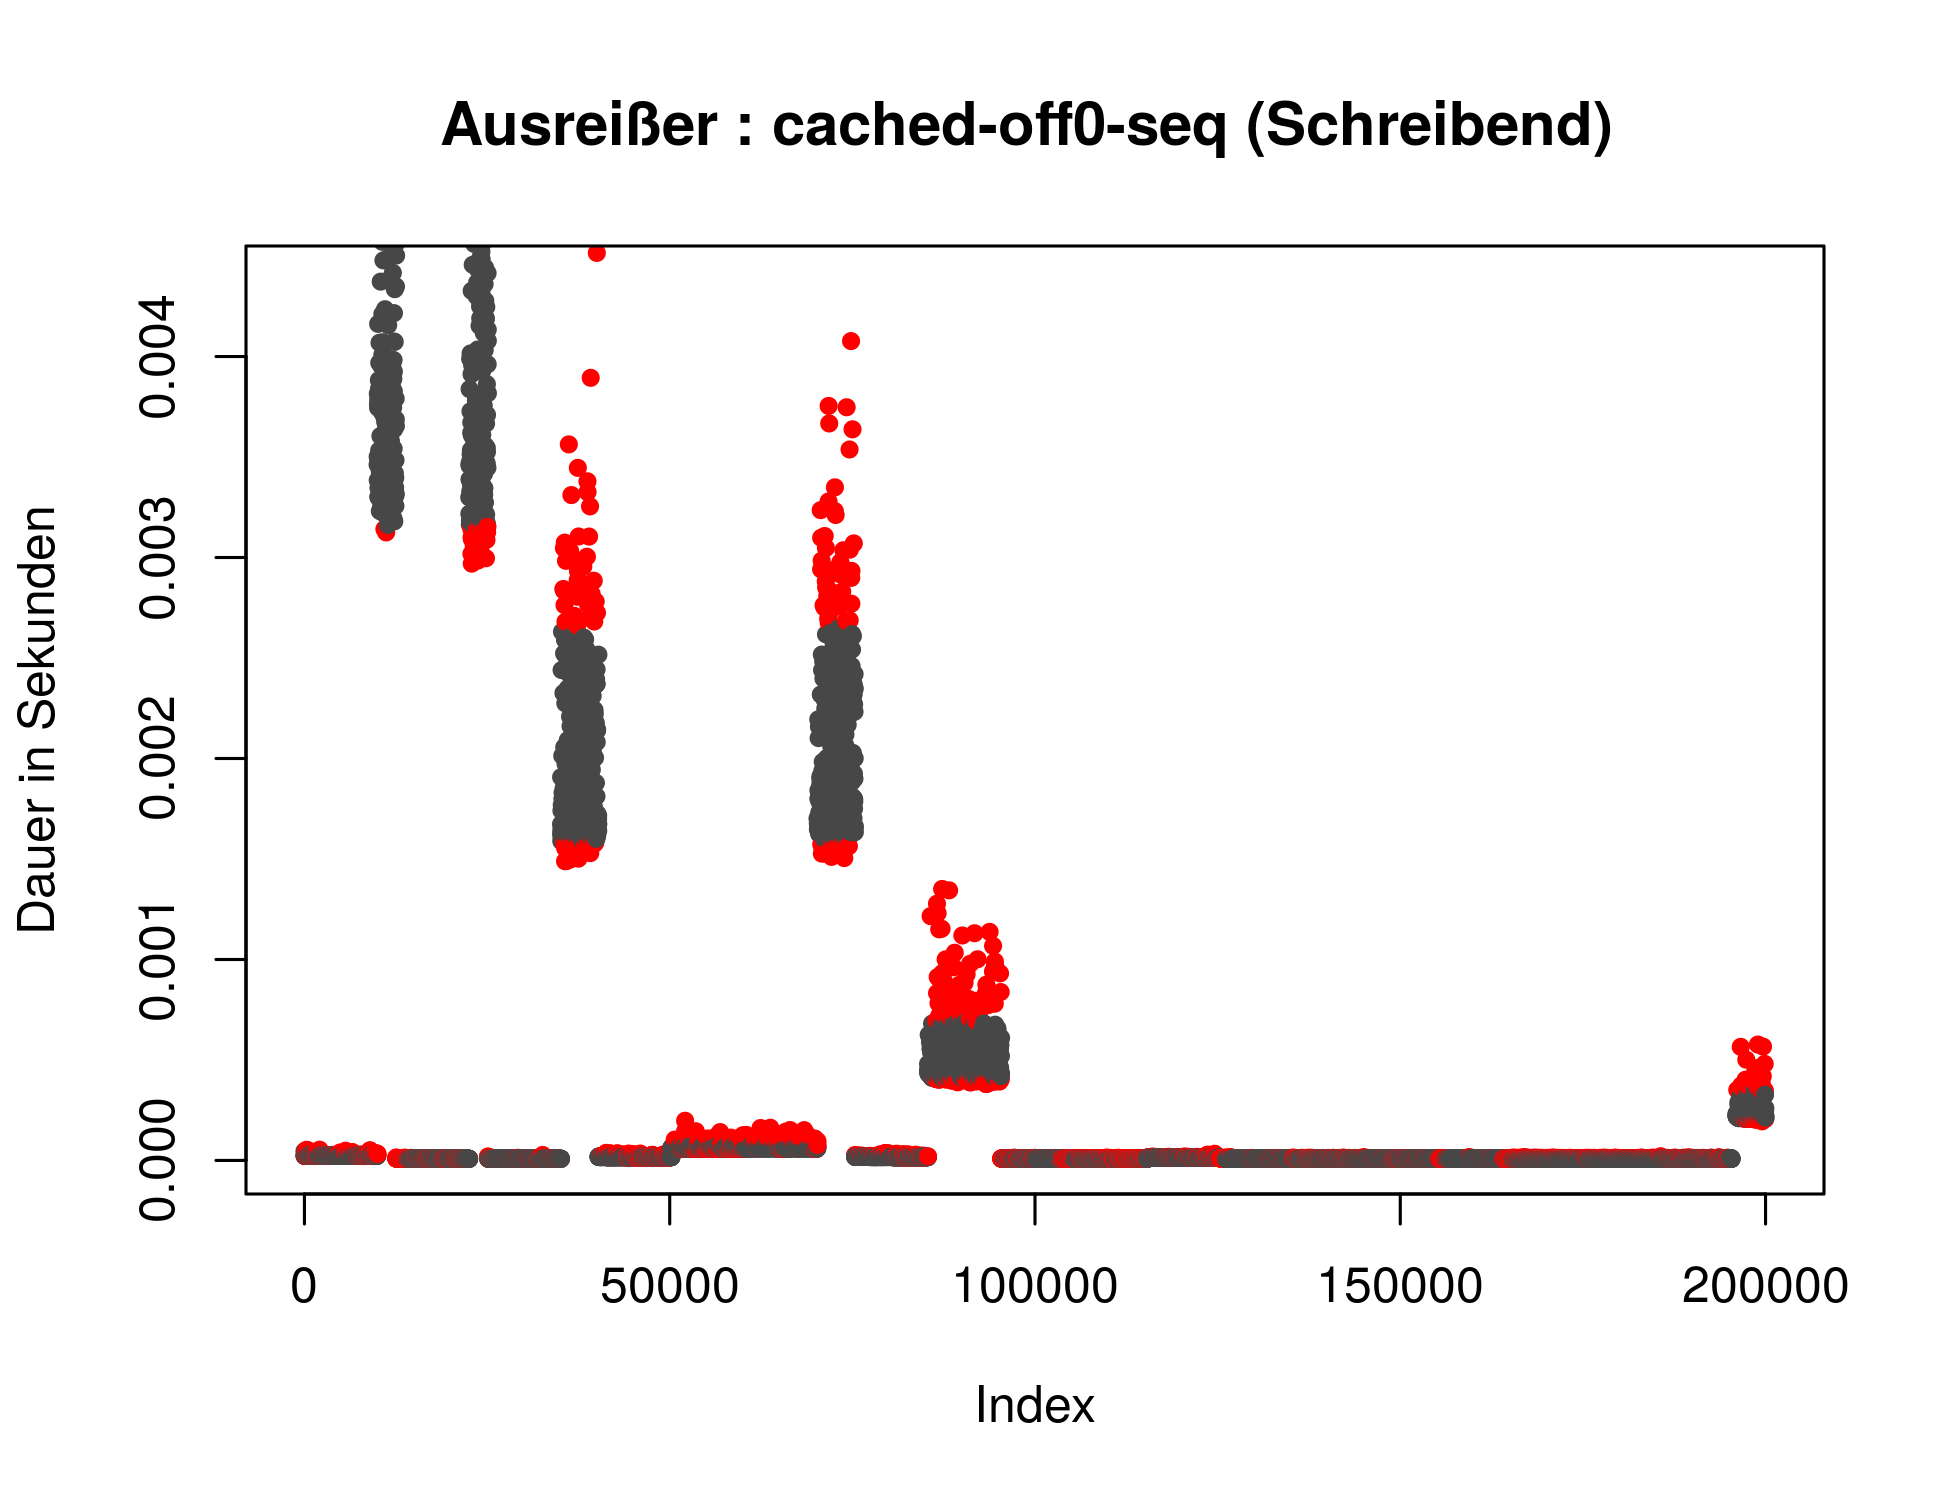
\includegraphics[width=.46\textwidth]{Bilder/Plots/exploration/plot_outlier_write_seq.png}
	}	
	\caption{Darstellung der Ausreißer (rote markiert)}
	\label{fig:ausreisser}
\end{figure} 

\subsubsection{Betrachtung der Laufzeiten pro Zugriffsgröße}
Um die unterschiedlichen Laufzeiten innerhalb einer Zugriffsgröße zu untersuchen, habe ich in den Abbildungen von \ref{fig:groesse1} bis \ref{fig:groesse2097152} für die Größen 1\,B, 16\,KiB und 2\,MiB alle Messungen zu diesen Größen betrachtet.
In den Graphen ist gut zu erkennen, dass die Varianz der Laufzeiten im sequentiellen Fall wesentlich geringer ausfällt, als bei den randomisierten Messungen.
Teilweise lassen sich die verschiedenen Messreihen (eine Messreihe umfasst 10\,000 Messungen, außer im 2\,MiB Fall, dort sind es 5000) am Muster der Zugriffszeiten voneinander unterscheiden.
So ist beispielsweise eine Verschiebung des Musters bei \ref{fig:groesse16384}c nach 10\,000 und 20\,000 Messungen deutlich zu erkennen.
Abhängig vom Systemzustand zum Beginn der Messreihe konnten die Anfragen also im Mittel unterschiedlich schnell bearbeitet werden.
In einigen Bildern lassen sich auch kurzzeitige Maxima oder Minima zwischen den Messreihen feststellen.
Beim sequentiell lesenden Fall für ein Byte (Abbildung \ref{fig:groesse1}a) dauern die ersten Messungen jeweils wesentlich länger, bis sich ein niedriger Wert eingependelt hat. Es könnte sein, dass hier nach einigen Zugriffen die Read-Ahead Caching-Strategie greift, die geforderten Daten befinden sich dann im Moment der Anfrage bereits im Cache. Dies macht auch Sinn, da sehr gut vorhersehbar ist, auf welche Daten beim sequentiellen Zugriff als nächstes zugegriffen werden.\\
Für die randomisierten Zugriffe ist der nächste Zugriffsort nicht vorhersehbar, sodass ein solches Verhalten, wie es bei SEQ beobachtet wurde, nicht möglich ist und es kann auch in keiner Abbildung erkannt werden.\\
Ein interessantes Verhalten kann in Abbildung \ref{fig:groesse16384}a beobachtet werden.
Zu Beginn jeder Messreihe werden die ersten E/A-Zugriffe zuverlässig sehr schnell ausgeführt, dann steigt die mittlere Zugriffszeit rapide an und oszilliert stark.
Möglicherweise wird in diesem Fall solange der Arbeitsspeicher aufgefüllt bis der Platz nicht mehr ausreicht und aufwendigere Speicherverwaltungen Platz für die neuen Daten im Speicher schaffen müssen.

\begin{figure}[b!]
	\centering
	\subfloat[SEQ-R]{
		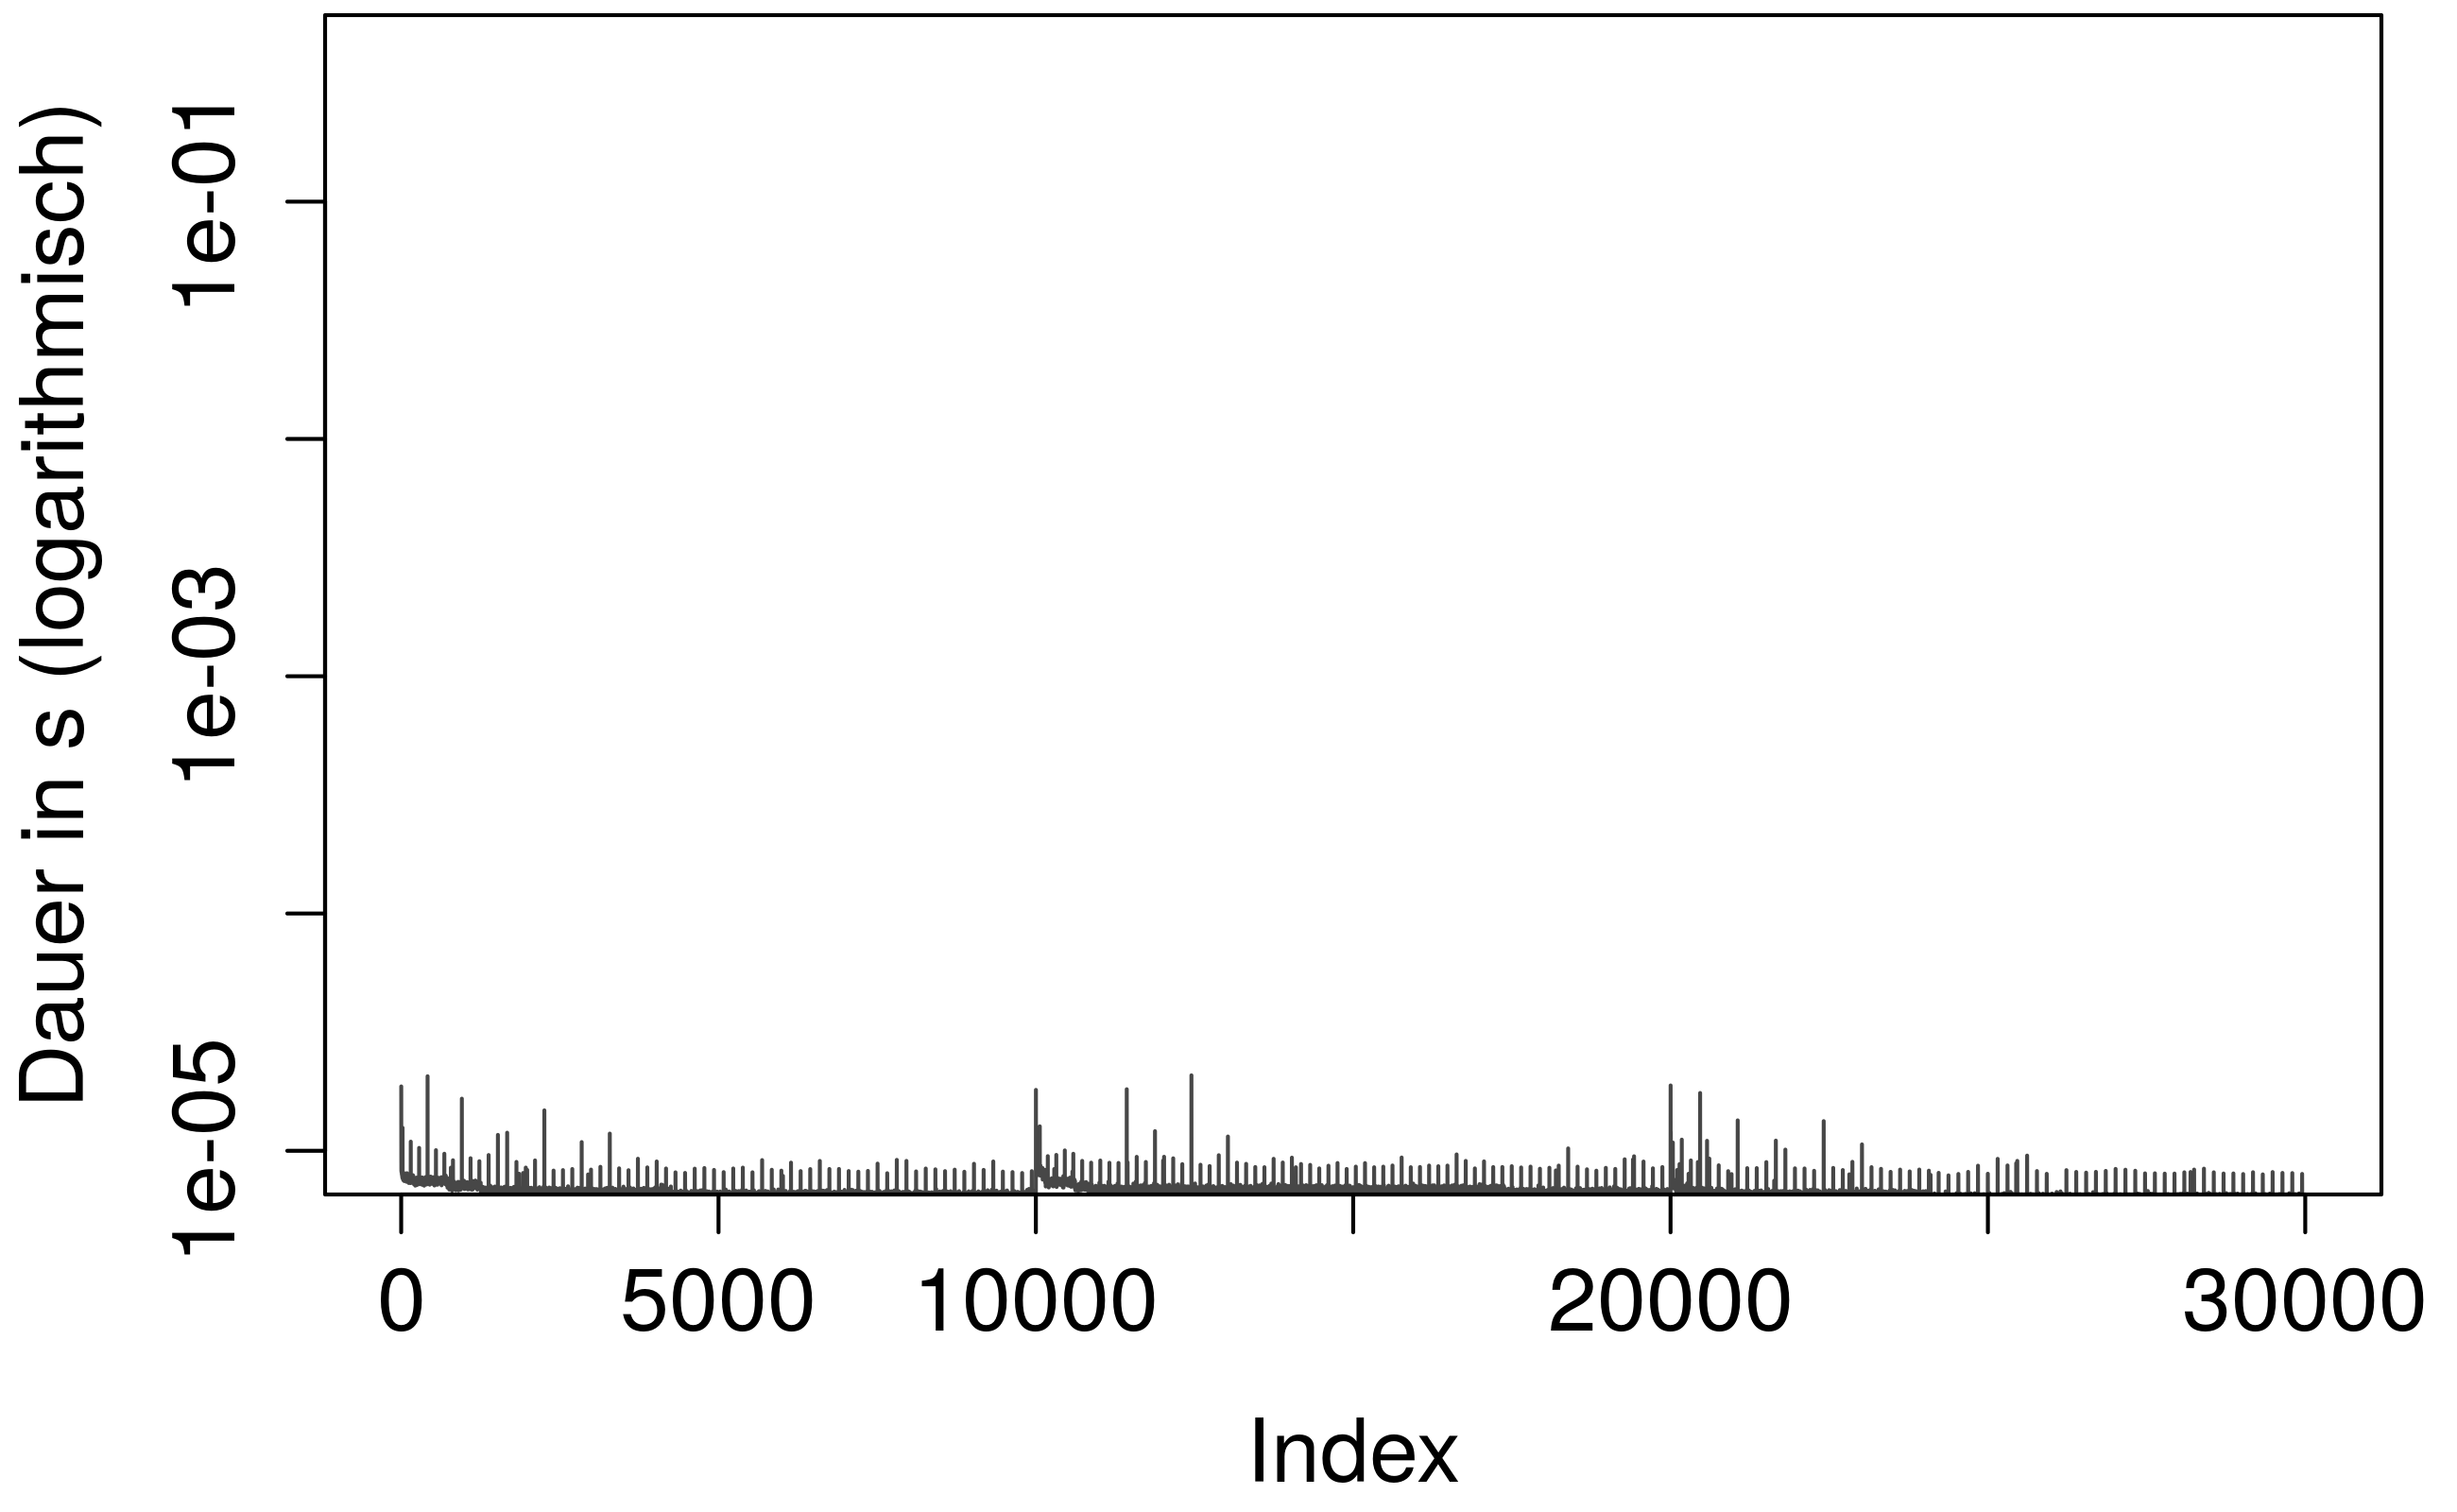
\includegraphics[width=.42\textwidth]{Bilder/Plots/exploration/plot_Size1_read_seq.png}
	}
	\hfill
	\subfloat[SEQ-W]{
		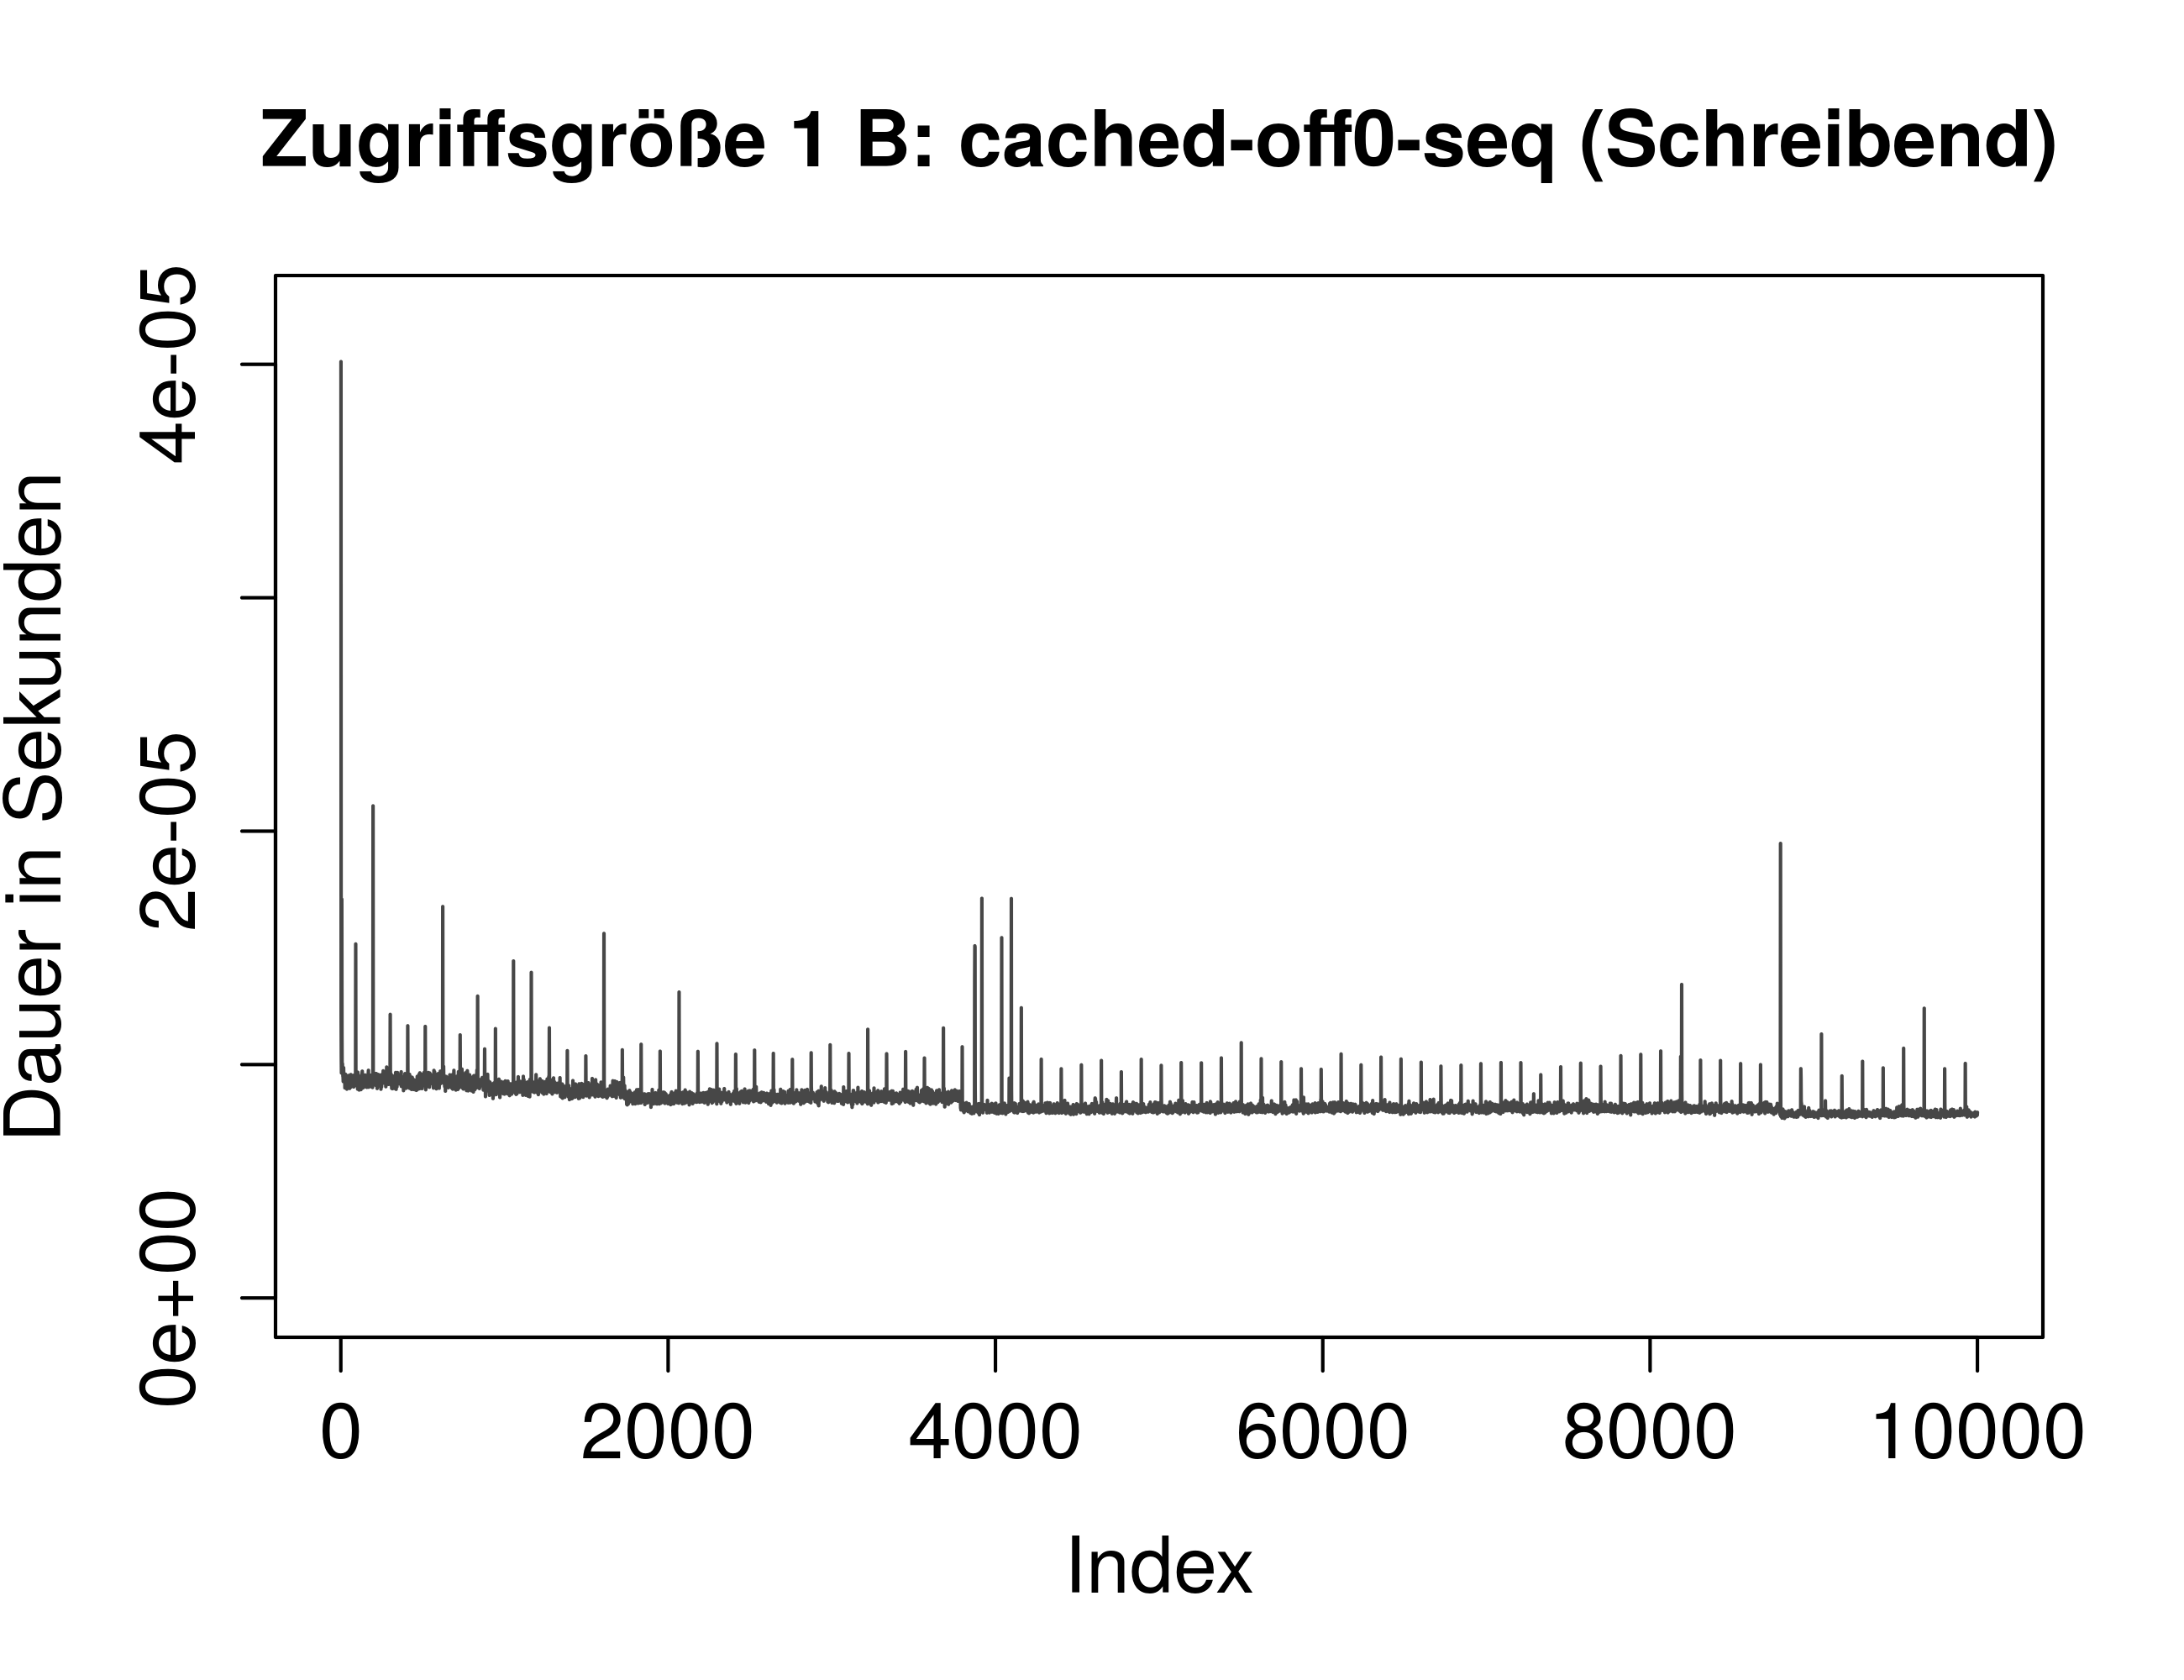
\includegraphics[width=.42\textwidth]{Bilder/Plots/exploration/plot_Size1_write_seq.png}
	}\\
	\subfloat[RND-R]{
		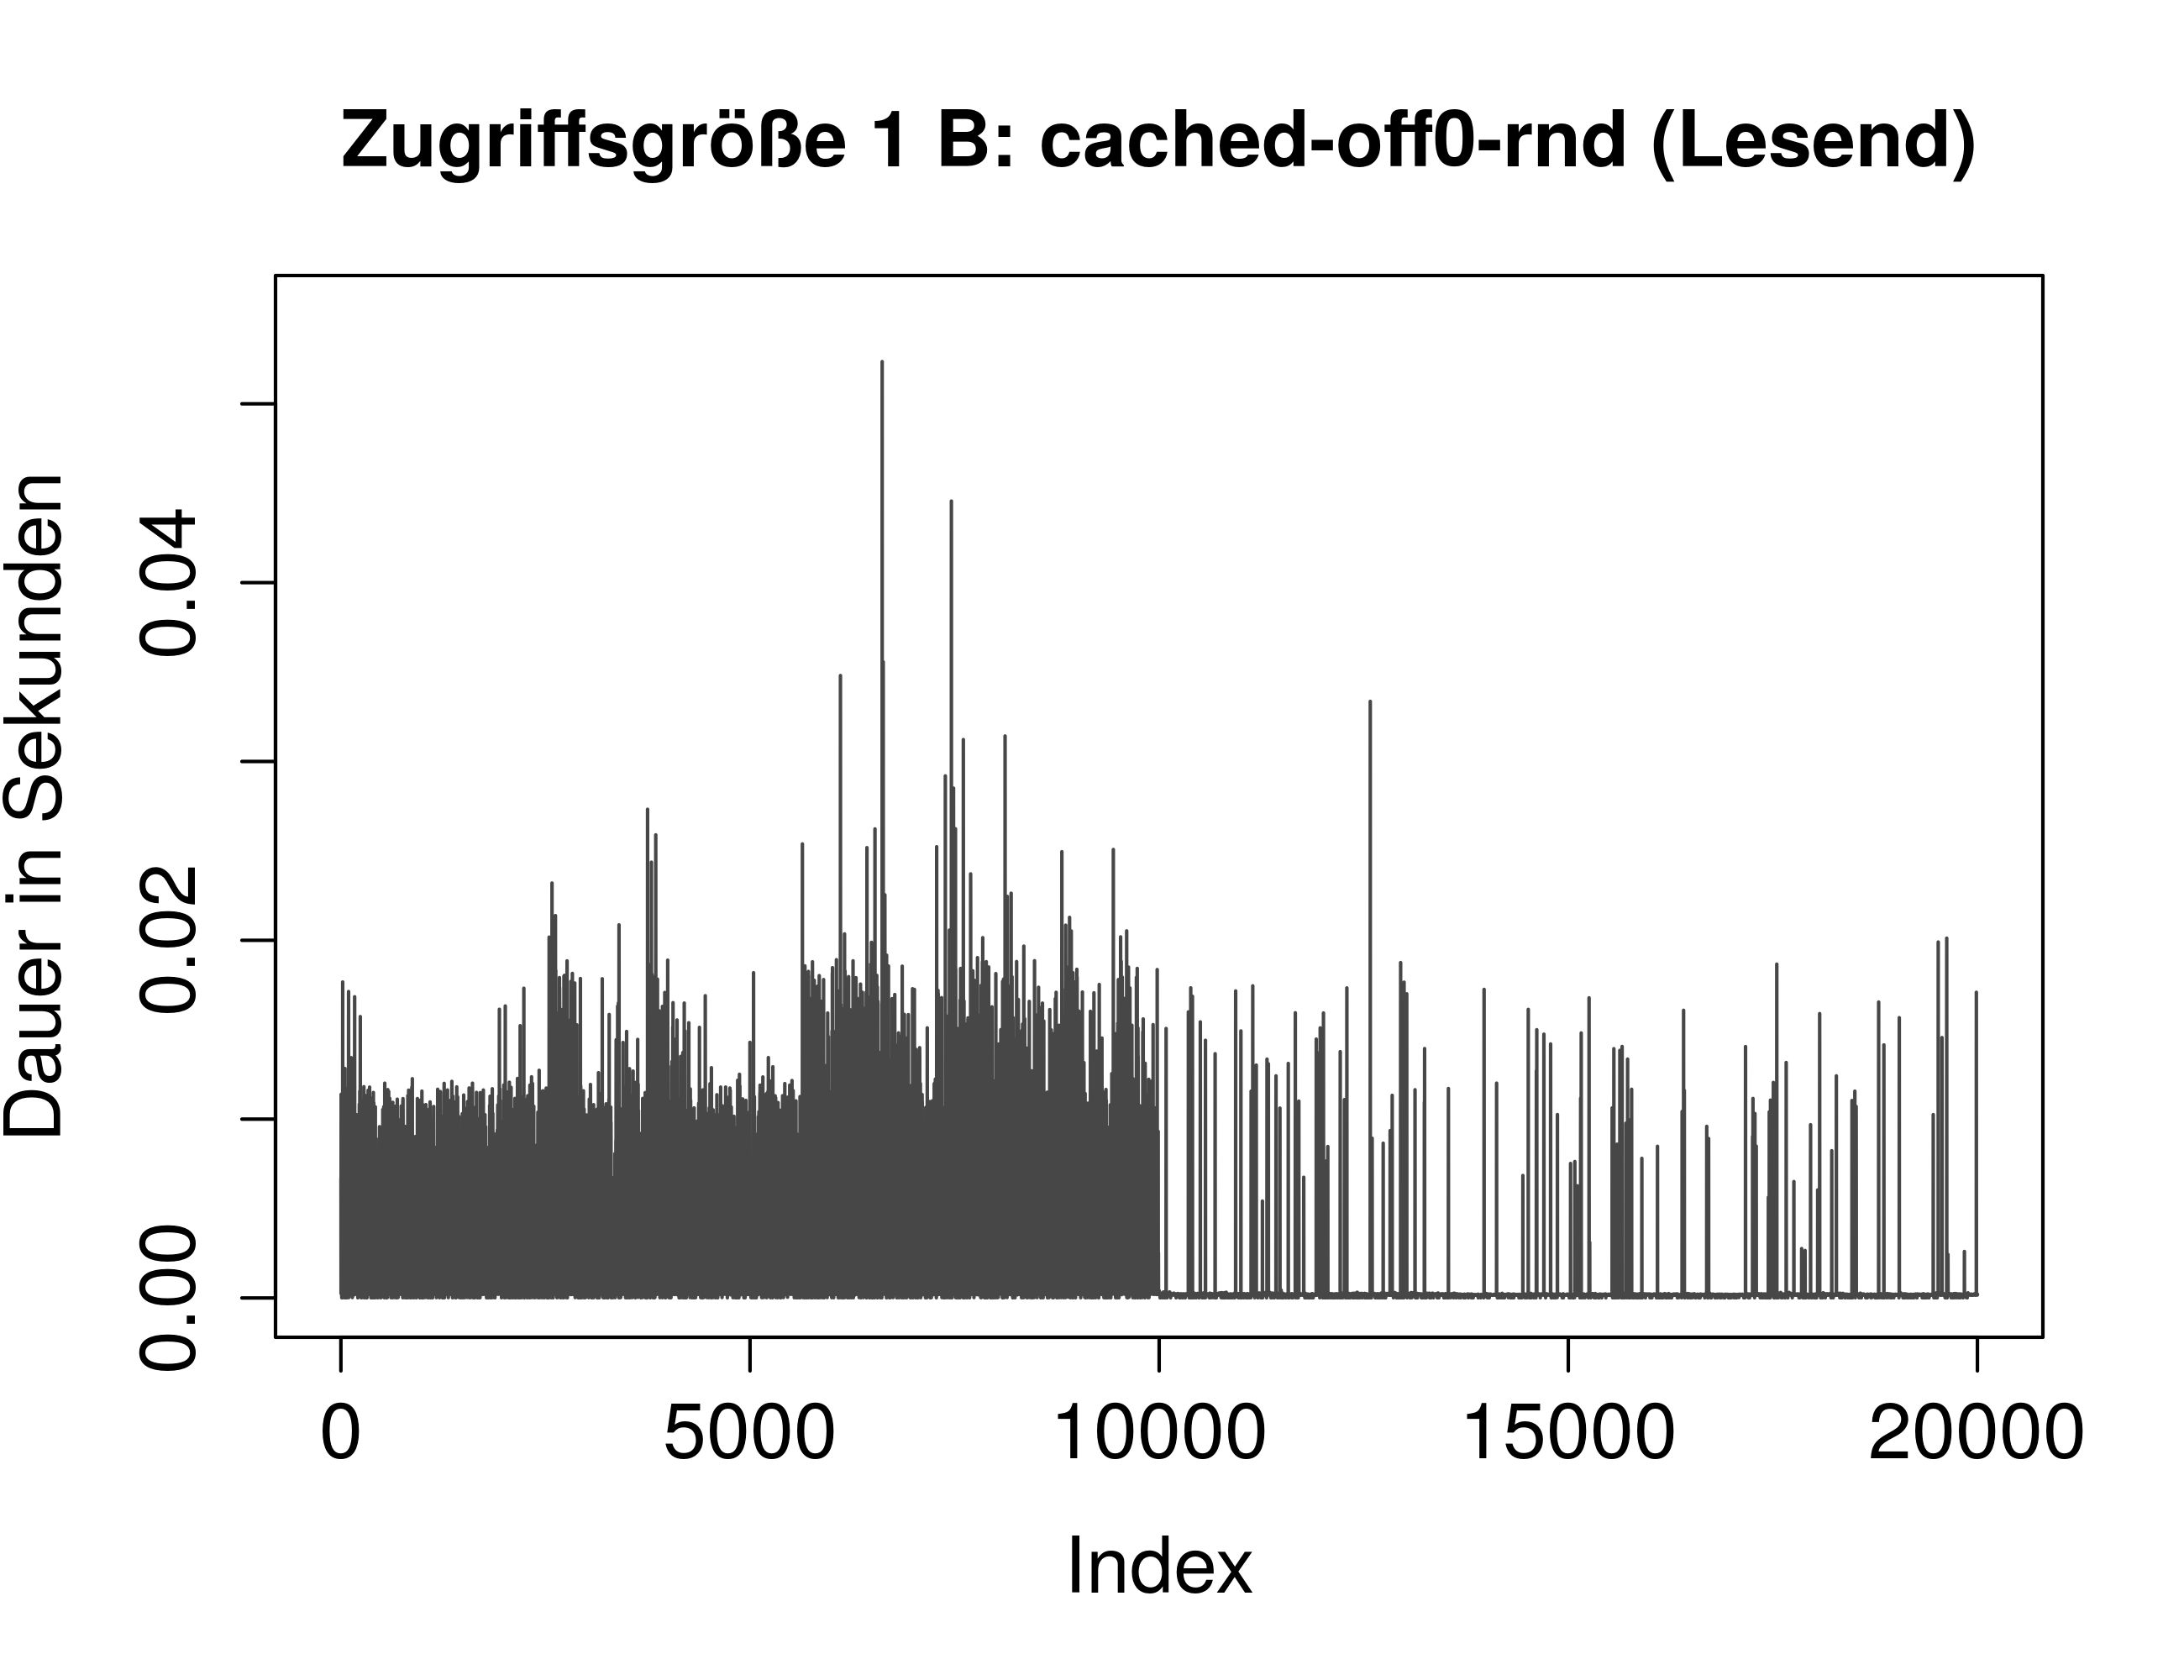
\includegraphics[width=.42\textwidth]{Bilder/Plots/exploration/plot_Size1_read_rnd.png}
	}
	\hfill
	\subfloat[RND-W]{
		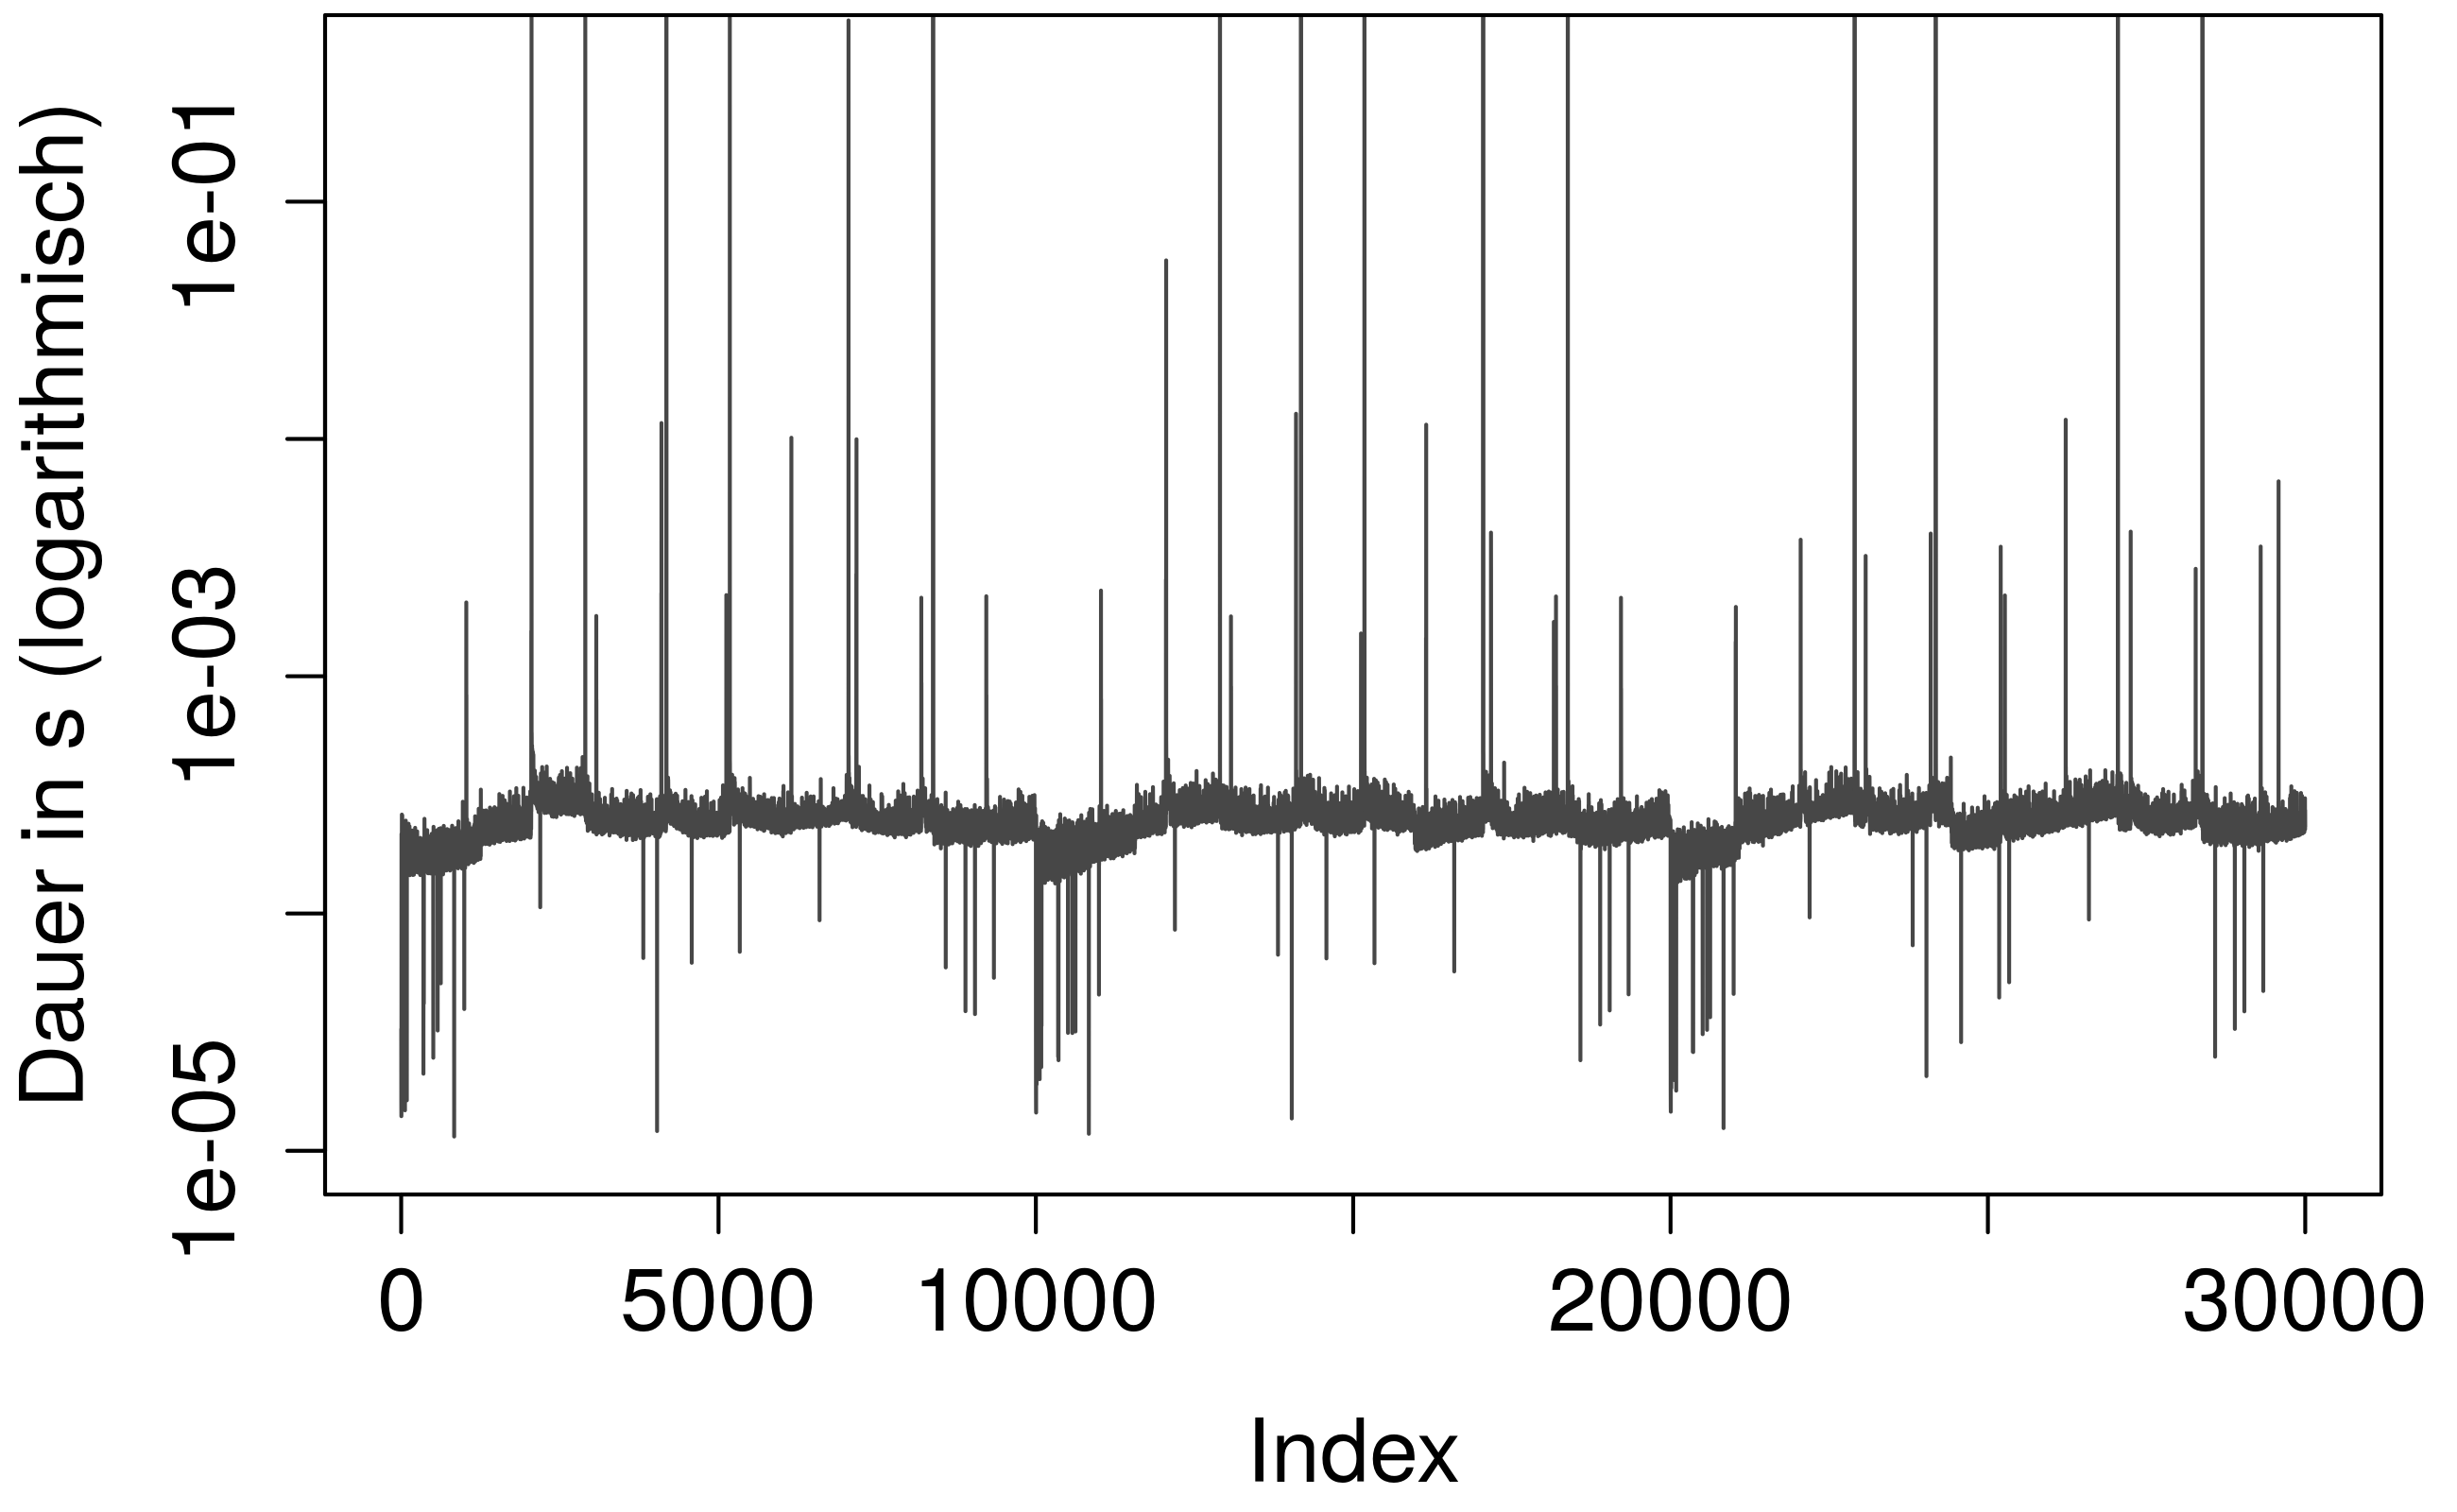
\includegraphics[width=.42\textwidth]{Bilder/Plots/exploration/plot_Size1_write_rnd.png}
	}
	\vspace*{-0.3cm}
	\caption{Detailbetrachtung aller Messungen mit Zugriffsgröße 1\,B}
	\label{fig:groesse1}
\end{figure}
\begin{figure}
	\centering
	\subfloat[SEQ-R]{
		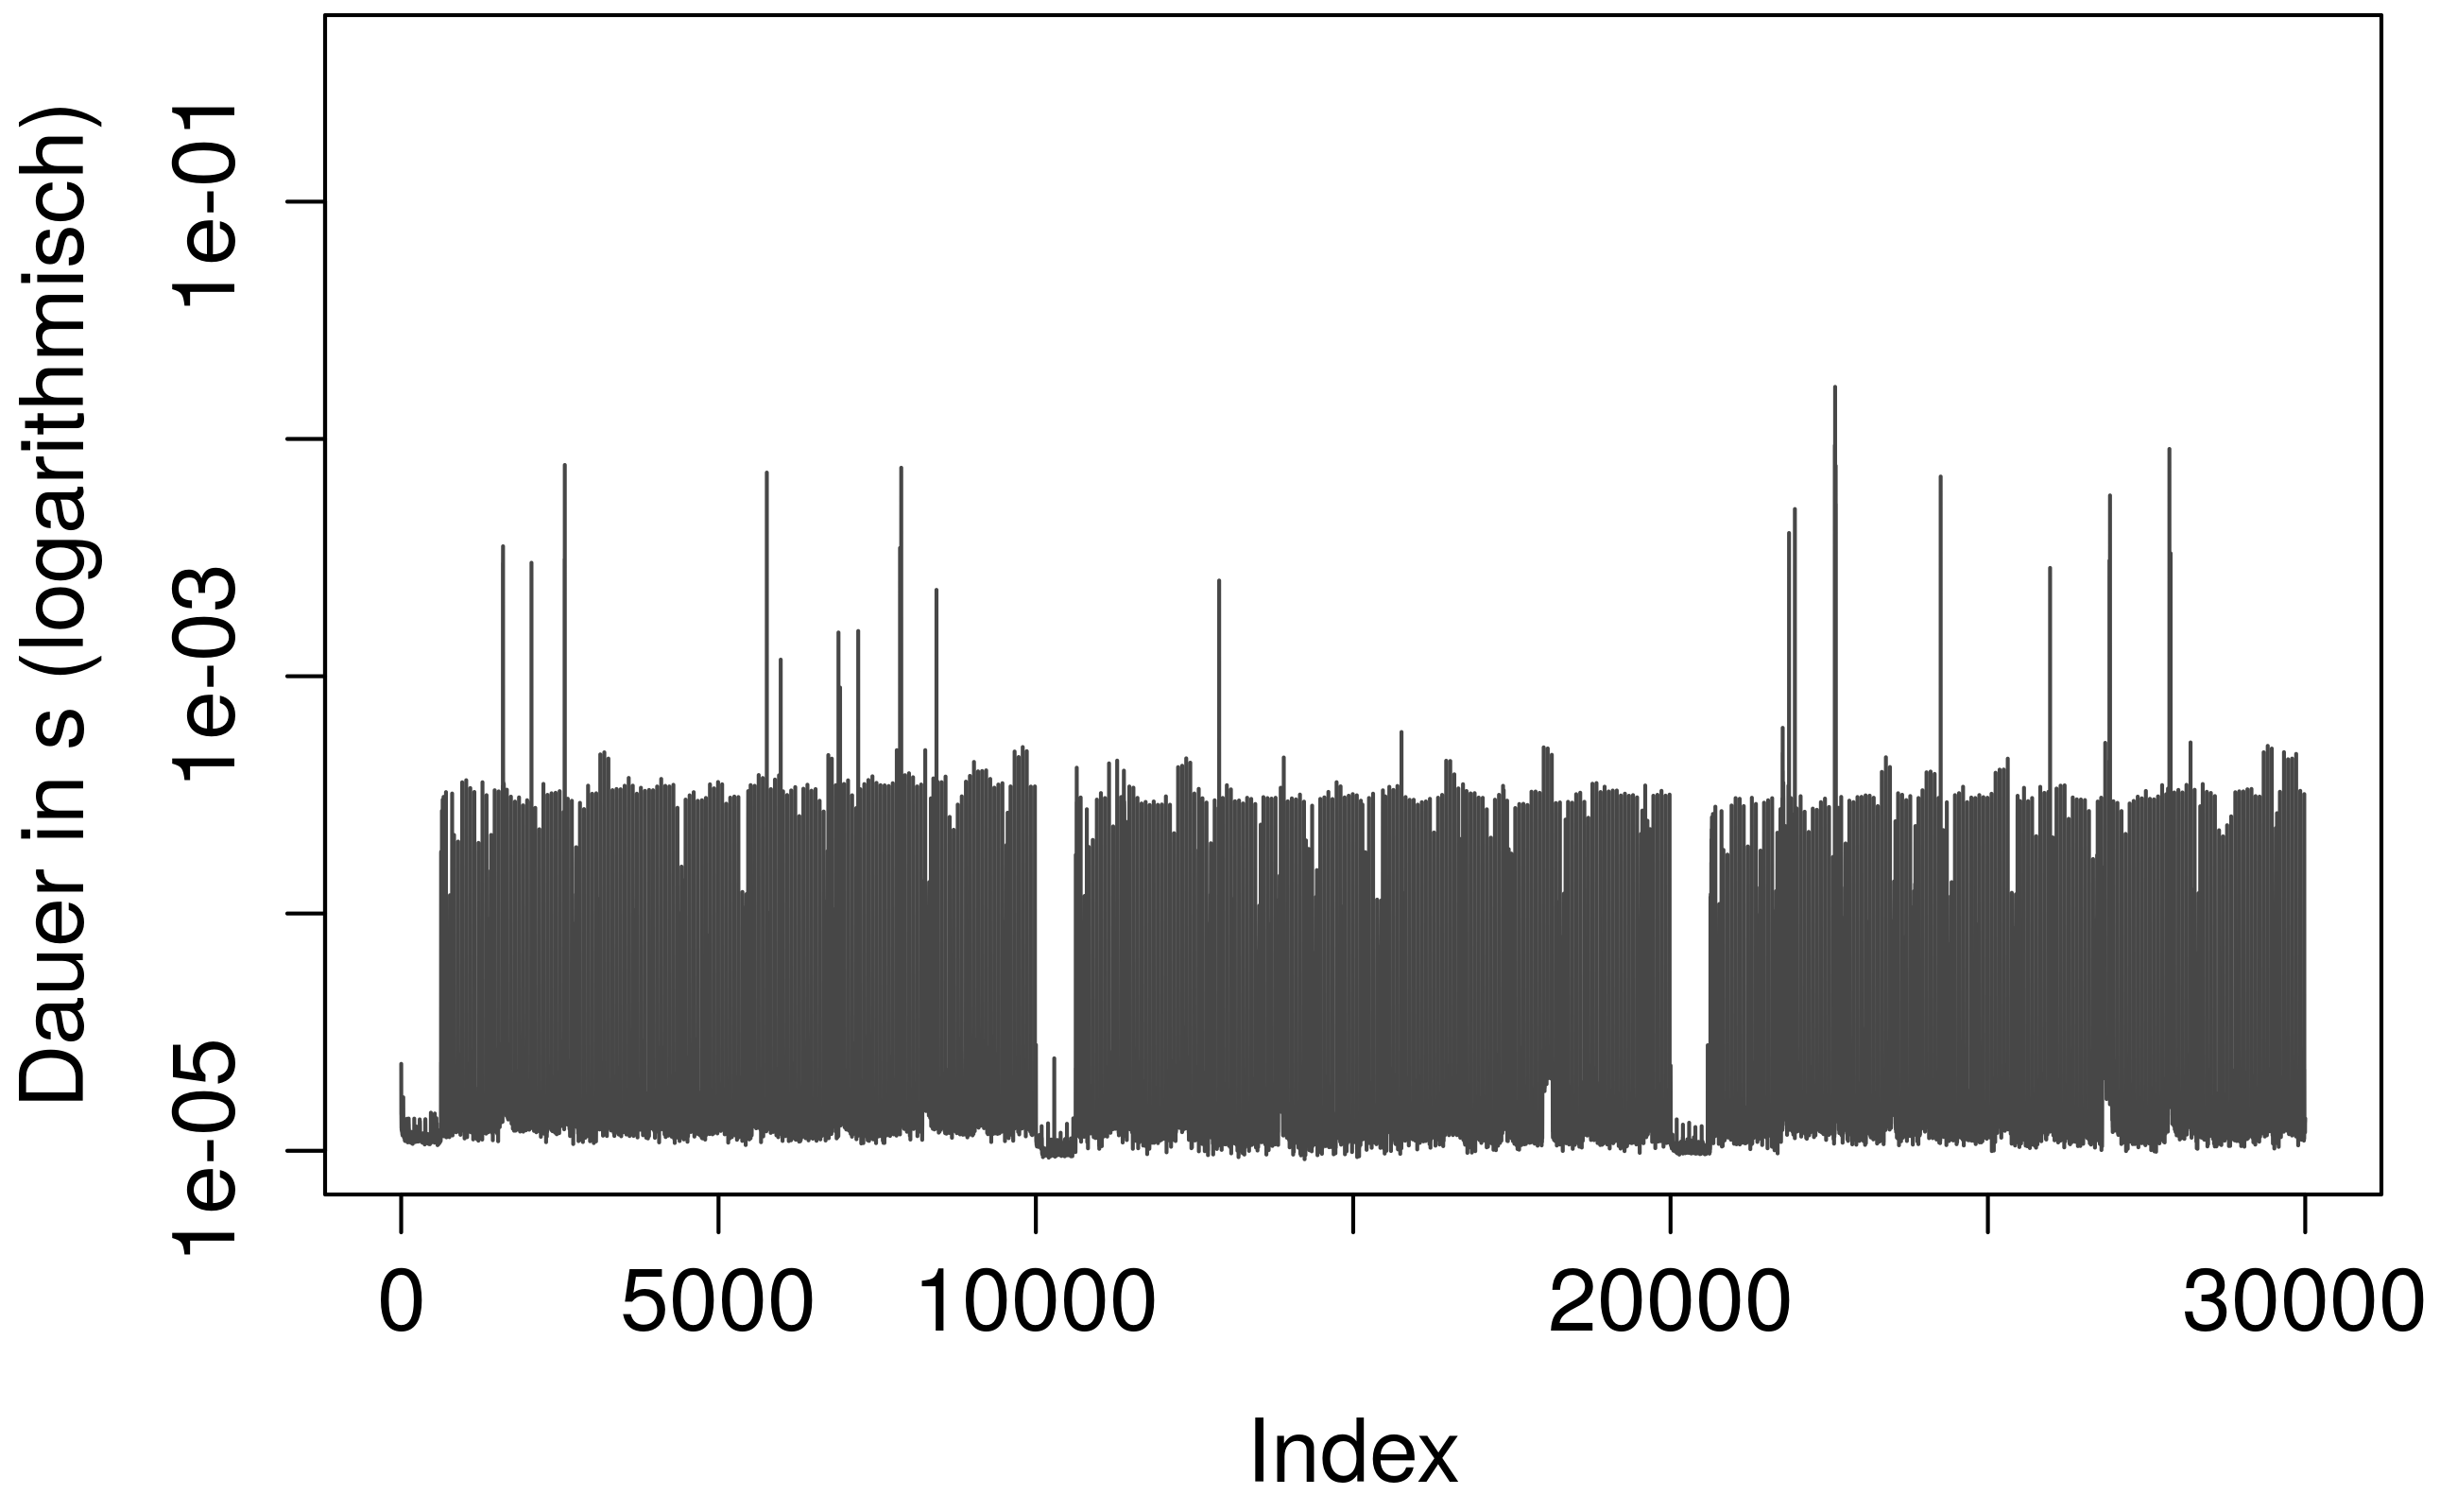
\includegraphics[width=.43\textwidth]{Bilder/Plots/exploration/plot_Size16384_read_seq.png}
	}
	\hfill
	\subfloat[SEQ-W]{
		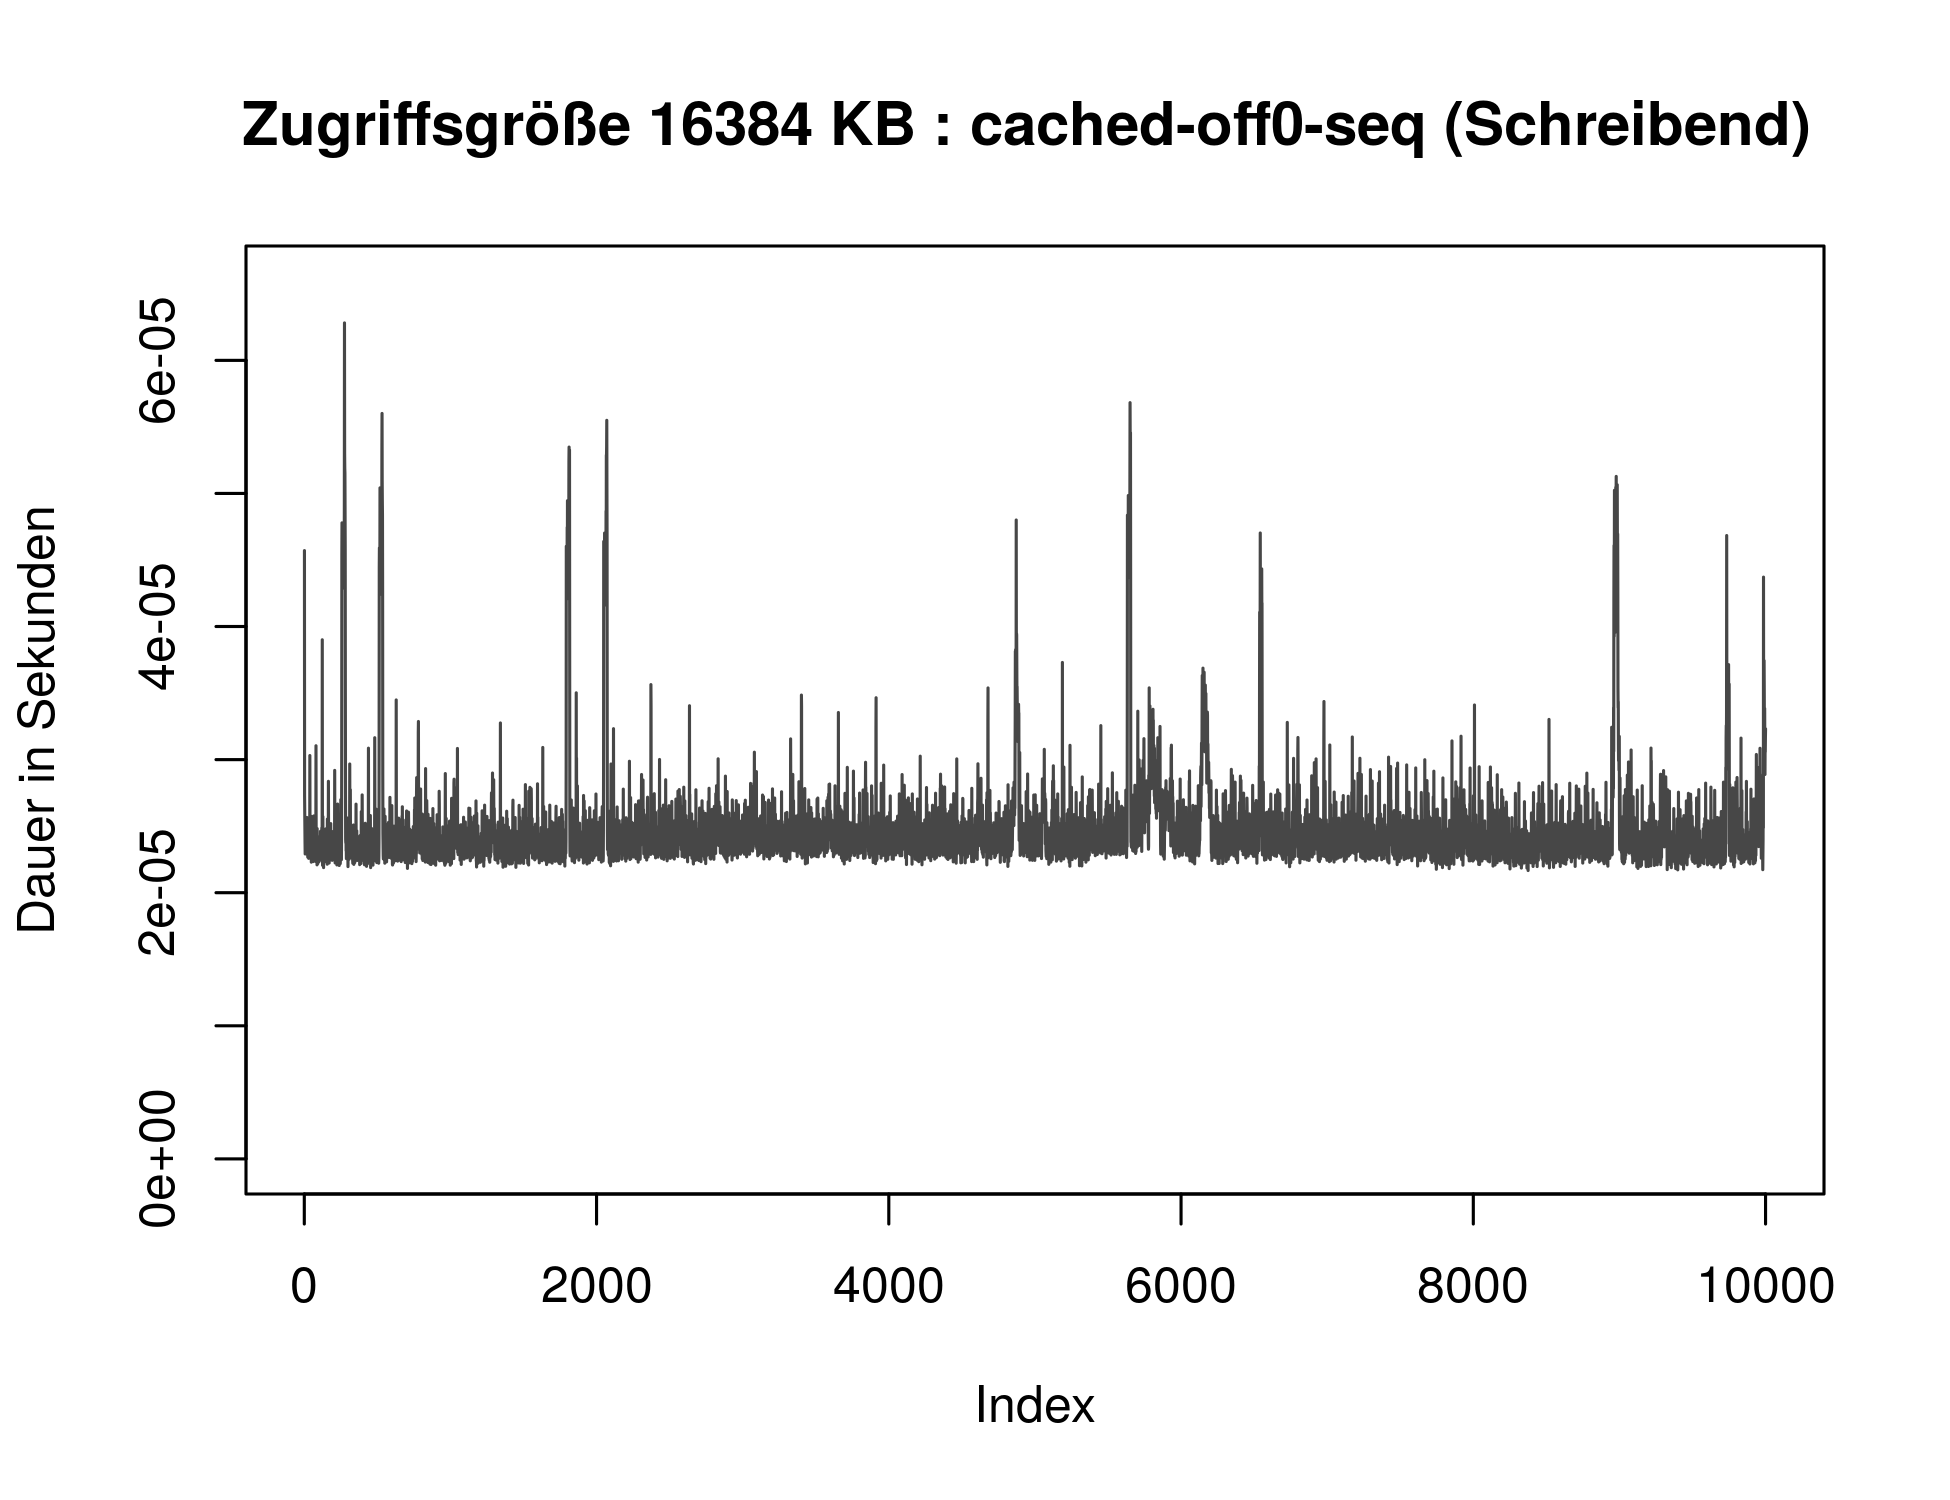
\includegraphics[width=.43\textwidth]{Bilder/Plots/exploration/plot_Size16384_write_seq.png}
	}\\
	\subfloat[RND-R]{
		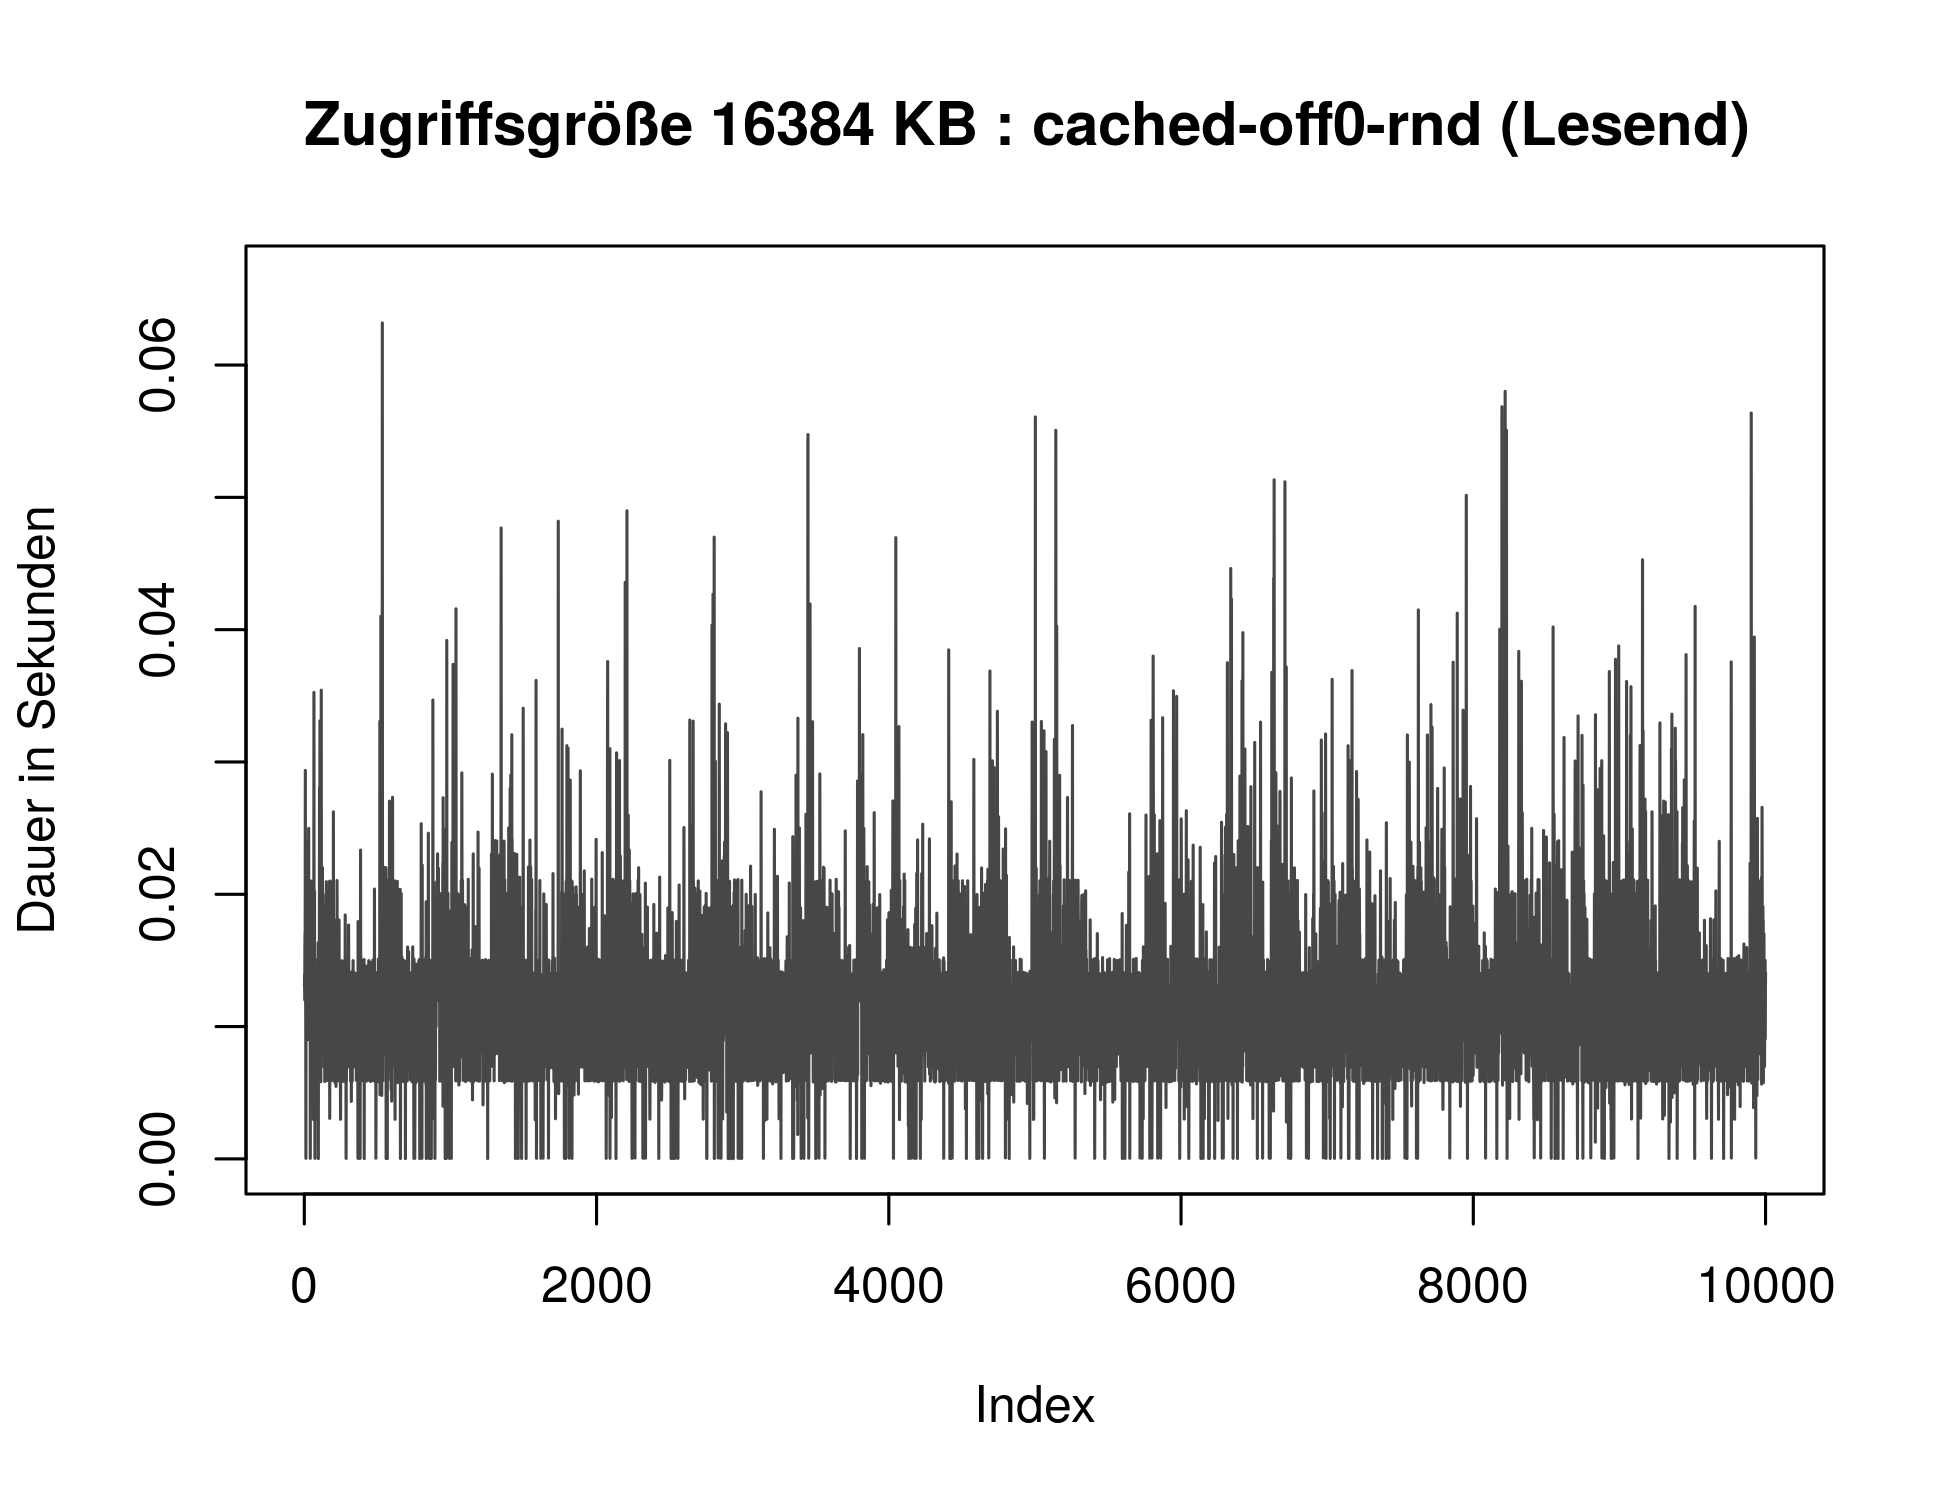
\includegraphics[width=.43\textwidth]{Bilder/Plots/exploration/plot_Size16384_read_rnd.png}
	}
	\hfill
	\subfloat[RND-W]{
		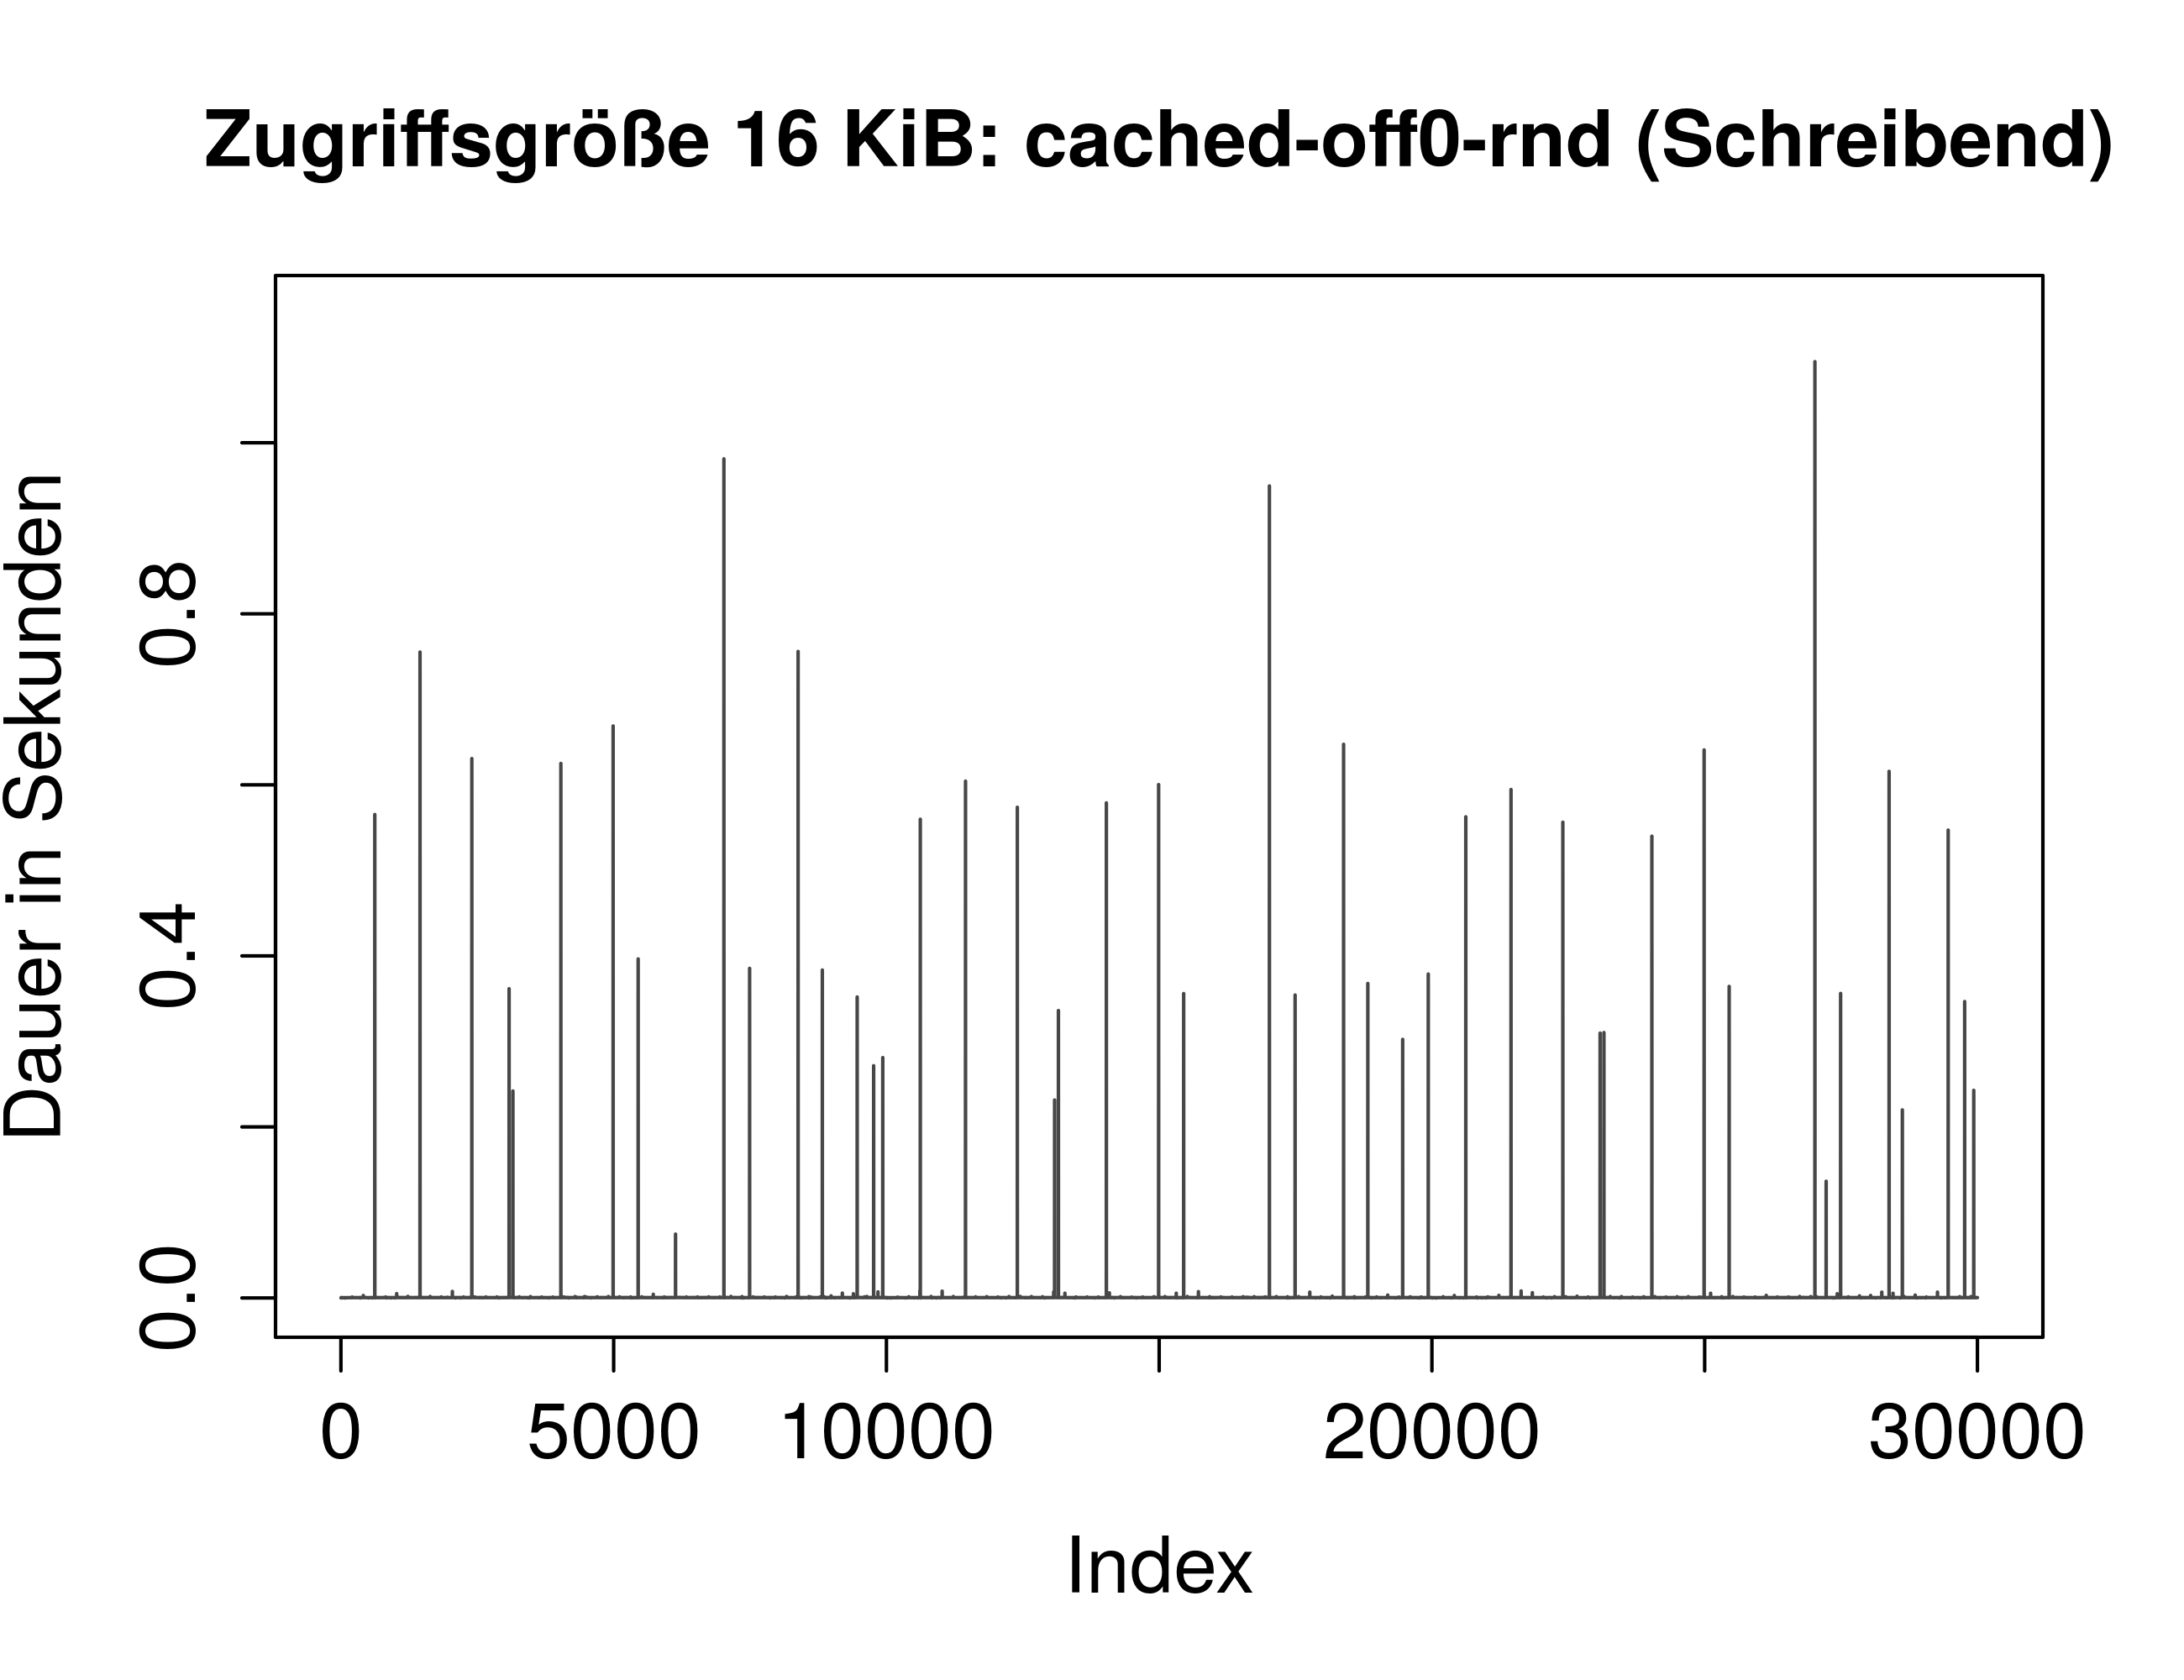
\includegraphics[width=.43\textwidth]{Bilder/Plots/exploration/plot_Size16384_write_rnd.png}
	}		
	\vspace*{-0.3cm}
	\caption{Detailbetrachtung aller Messungen mit Zugriffsgröße 16\,KiB}
	\label{fig:groesse16384}
\end{figure}
\begin{figure}
	\centering
	\subfloat[SEQ-R]{
		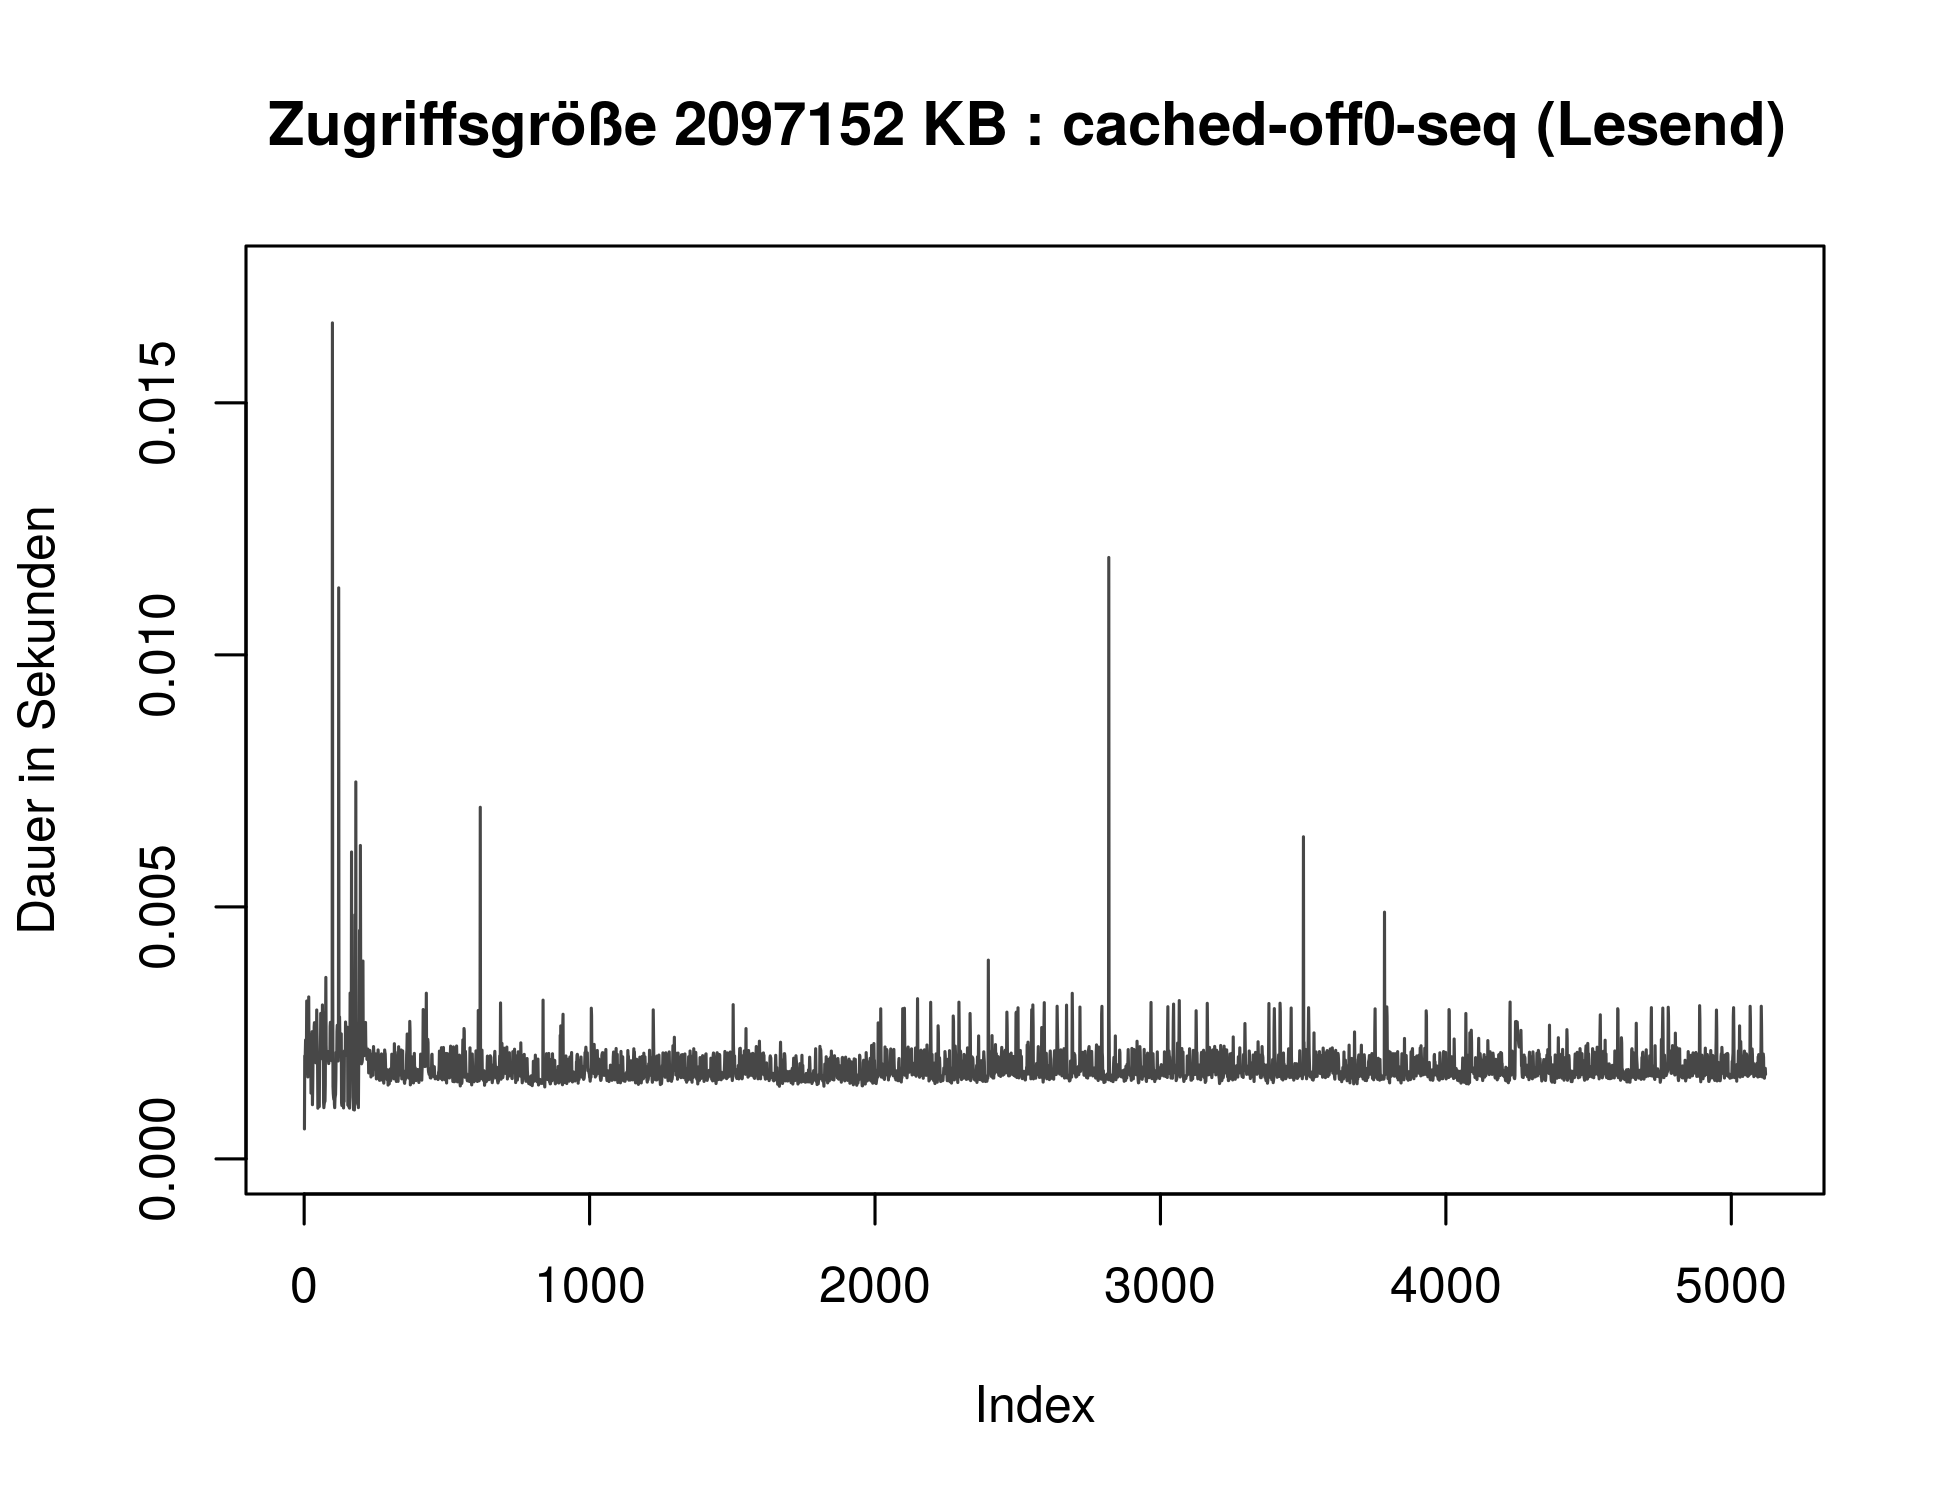
\includegraphics[width=.43\textwidth]{Bilder/Plots/exploration/plot_Size2097152_read_seq.png}
	}
	\hfill
	\subfloat[SEQ-W]{
		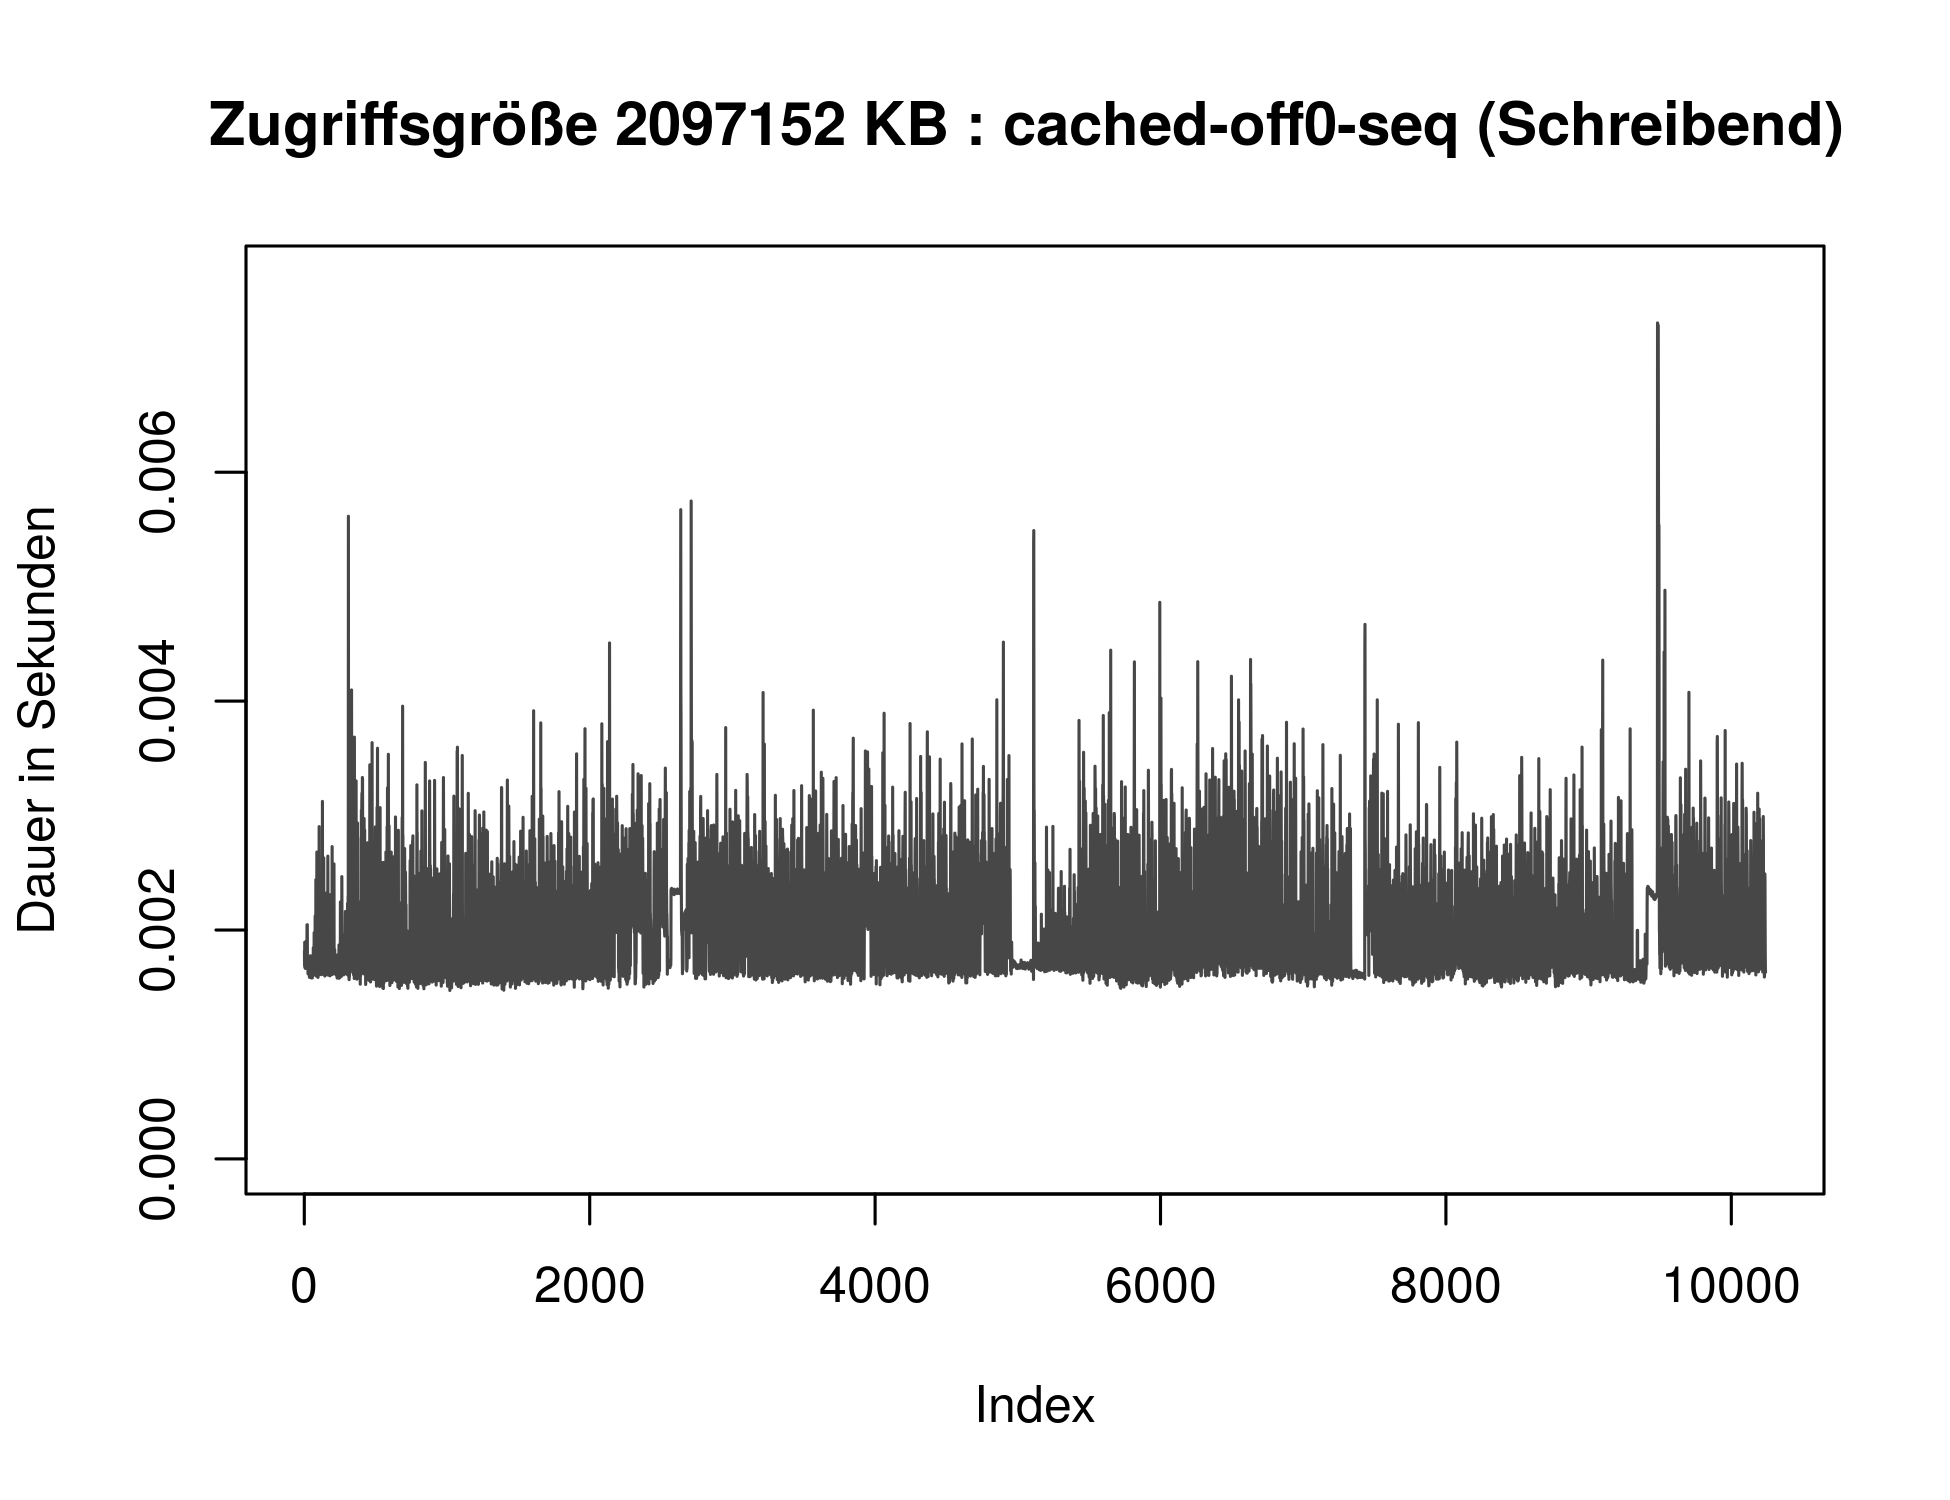
\includegraphics[width=.43\textwidth]{Bilder/Plots/exploration/plot_Size2097152_write_seq.png}
	}\\
	\subfloat[RND-R]{
		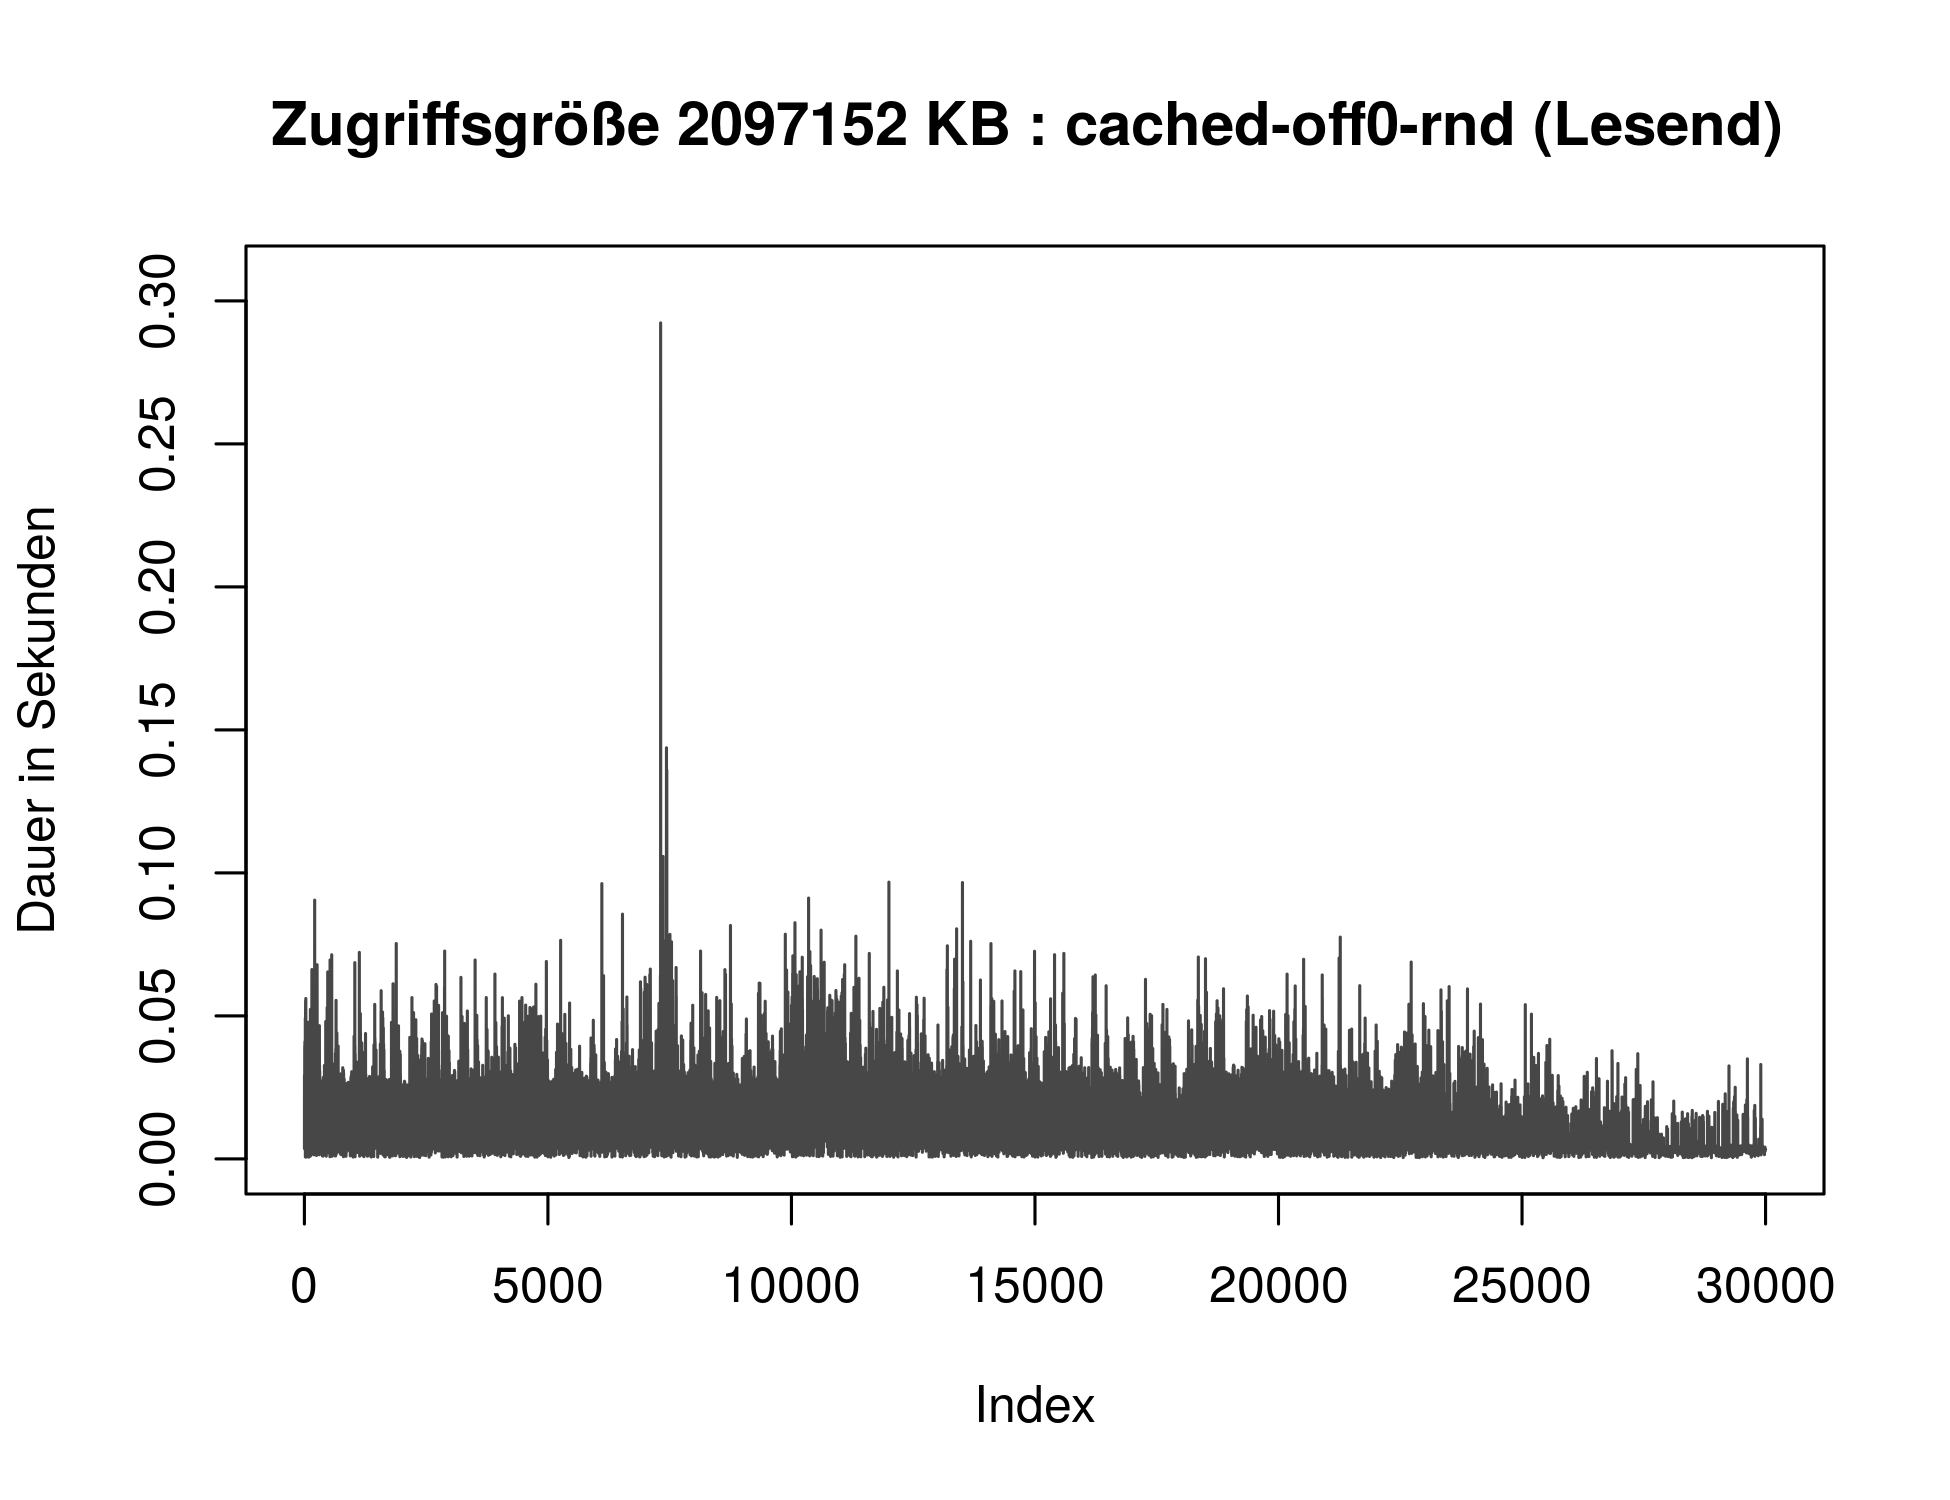
\includegraphics[width=.43\textwidth]{Bilder/Plots/exploration/plot_Size2097152_read_rnd.png}
	}
	\hfill
	\subfloat[RND-W]{
		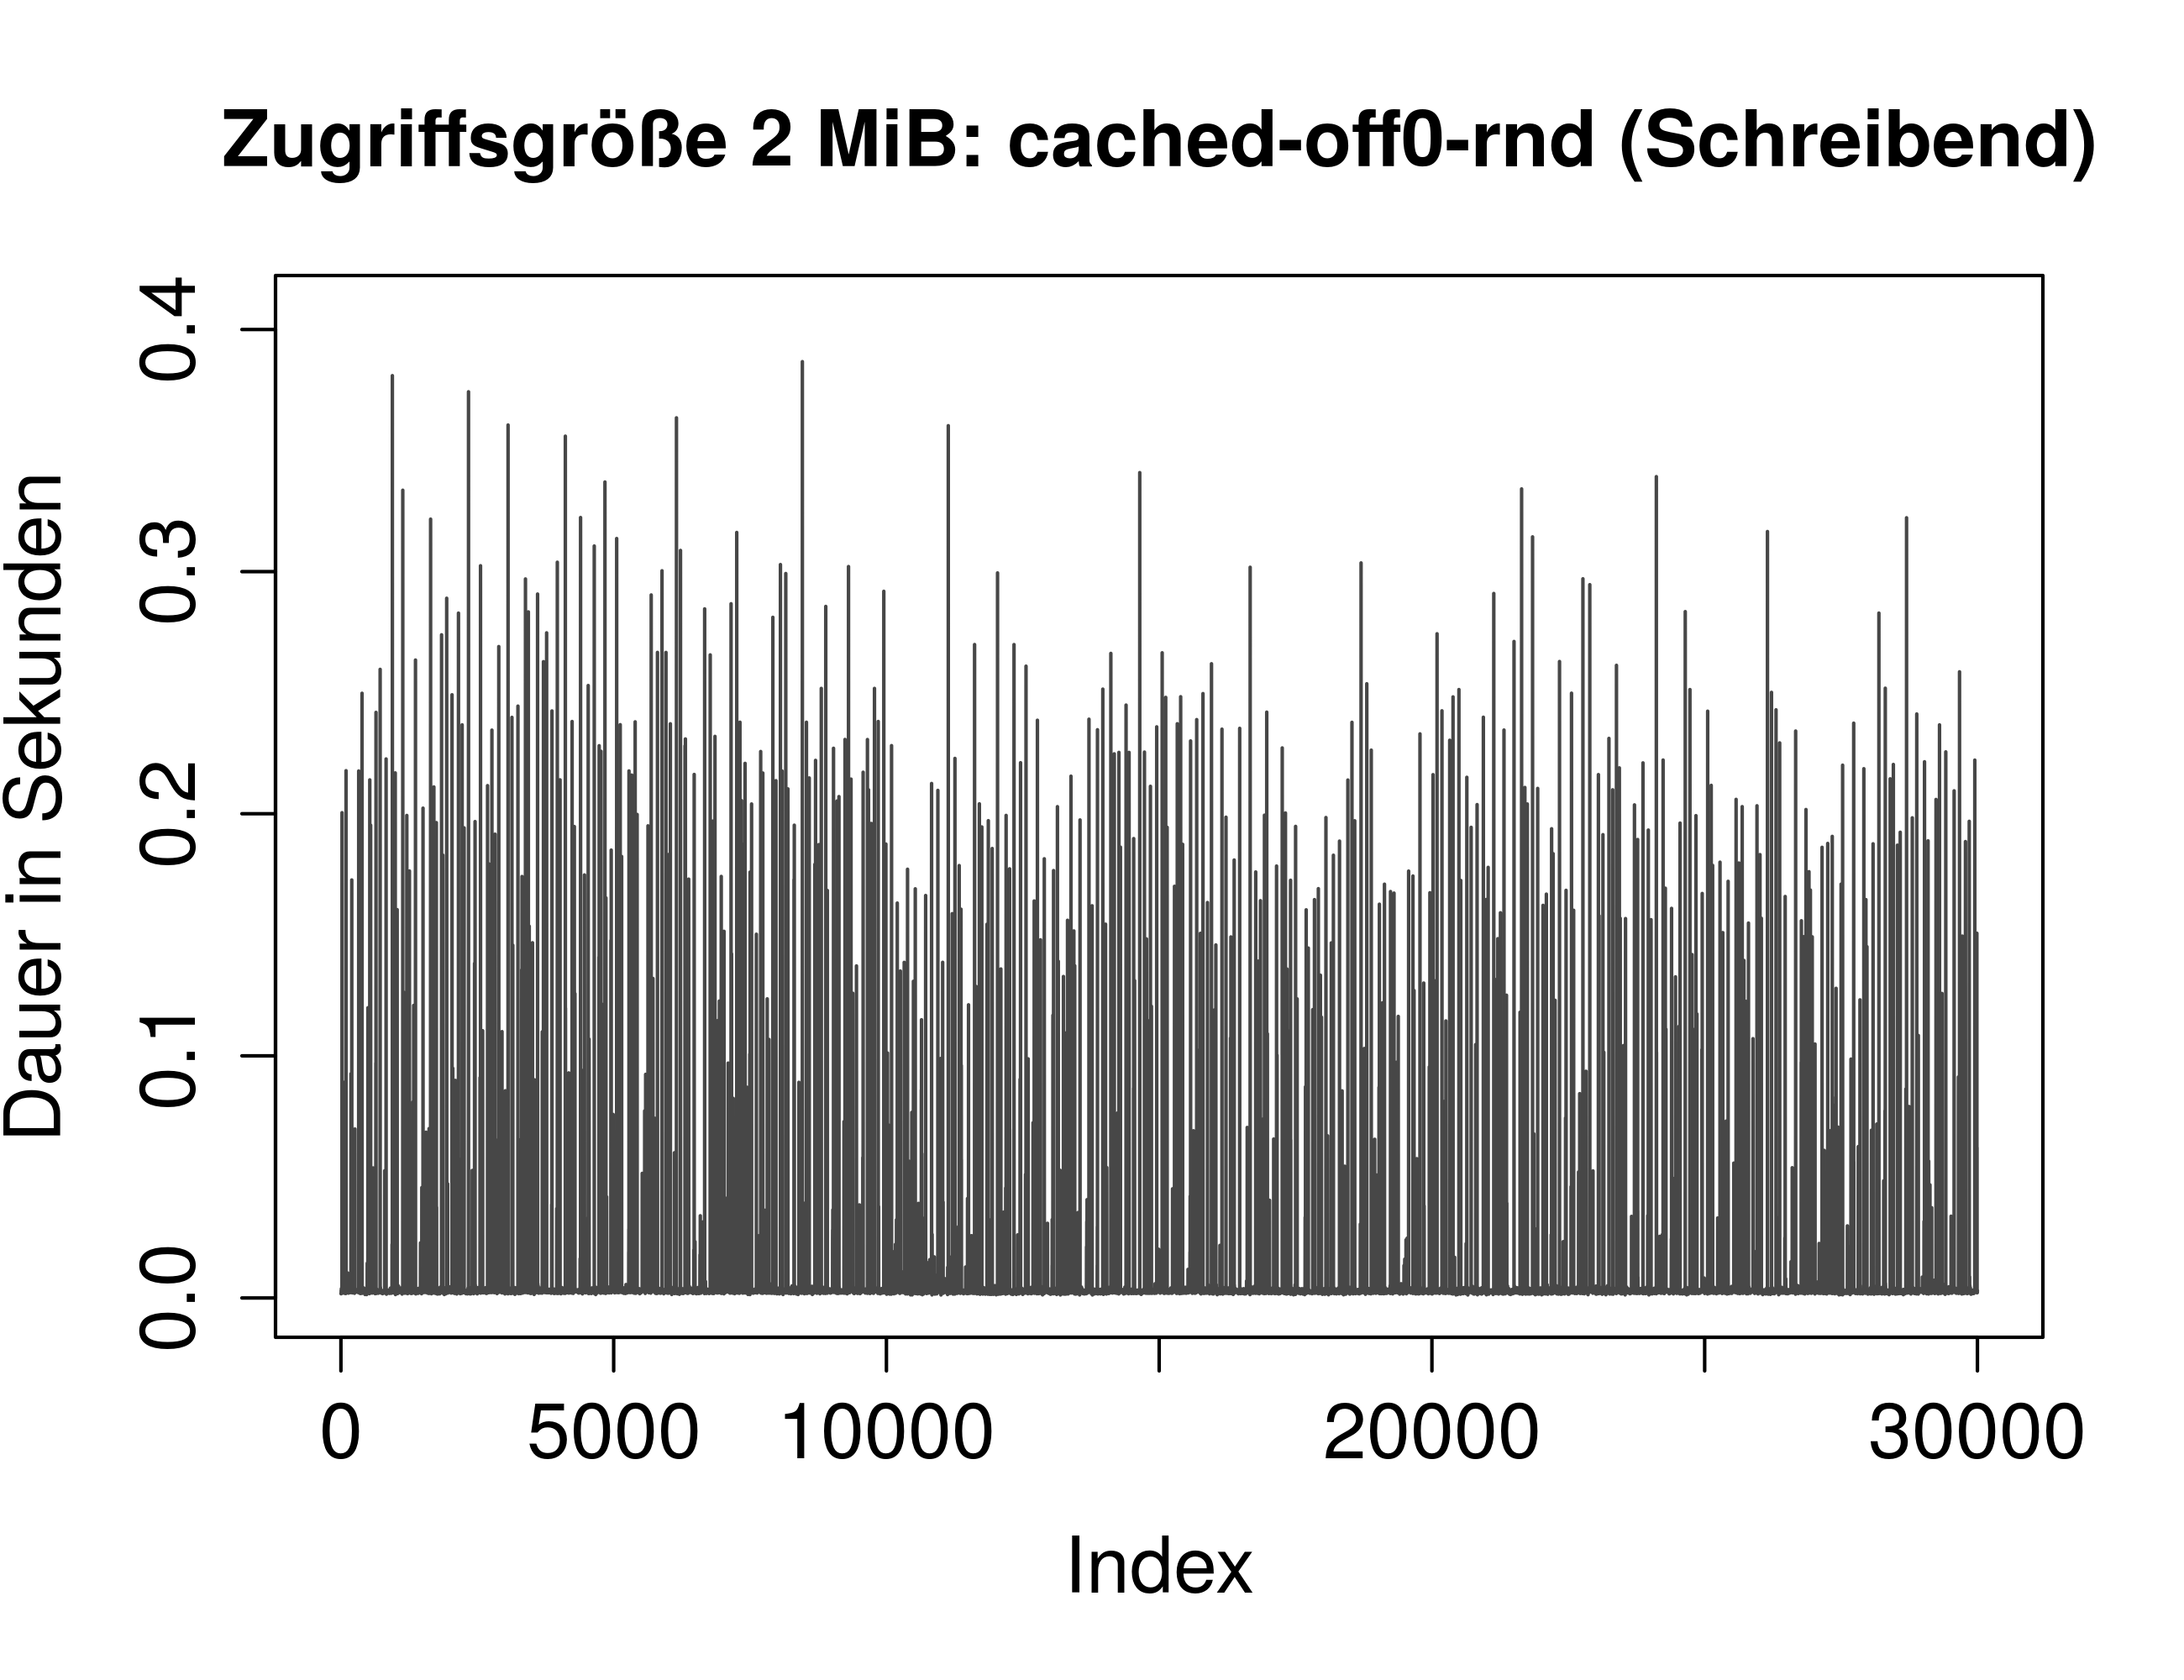
\includegraphics[width=.43\textwidth]{Bilder/Plots/exploration/plot_Size2097152_write_rnd.png}
	}		
	\vspace*{-0.3cm}
	\caption{Detailbetrachtung aller Messungen mit Zugriffsgröße 2\,MiB}
	\label{fig:groesse2097152}
\end{figure}
\clearpage
\subsubsection{Ausschnittweise Betrachtung der Messungen}
Um die Messdaten zur Untersuchung noch detaillierter darzustellen, müssen kleine Ausschnitte herausgegriffen werden. Zunächst betrachte ich die ersten $250$ Messungen jedes Experiments.
In der Abbildung \ref{fig:first250}b zum Datensatz SEQ-W scheint eine gewisse Periodizität der Zugriffszeiten vorhanden zu sein. Etwa alle 45 Messungen gibt es einen größeren Sprung, alternierend sind die Laufzeiten jeweils etwas langsamer und schneller.
Nach genau $123$ Punkten scheint sich das Muster zu wiederholen, dort befindet sich der zweitgrößte Messwert der Laufzeit in diesem Ausschnitt.\\
Ein erstes simples Modell könnte es nun sein, eine Fortführung der augenscheinlichen Periodizität anzuwenden, indem die ersten $123$ Zugriffszeiten für die Laufzeiten 123 bis 246 vorhergesagt werden.
Wenn man diese Vorhersagen jedoch über die tatsächlichen Zugriffszeiten legt (siehe Abbildung \ref{fig:periodicity}), so erkannt man doch, dass der Verlauf der Messungen von dieser Periode abweicht.\\ 
Bei den anderen Graphen kann keine so simple Periodizität beobachtet werden.
In den Graphen \ref{fig:first250}a und \ref{fig:first250}c sind besonders starke Ausreißer nach oben in den Laufzeiten zu erkennen. In Abbildung \ref{fig:first250}d sind dagegen einige Ausreißer, die wesentlich schneller bearbeitet wurden.\\
Einzelne sehr starke Ausreißer wie bei SEQ-R sind vermutlich durch außergewöhnlich große queue-Zeiten entstanden.
Regelmäßigere Ausreißer sind ein Zeichen für systematisch anders behandelte E/A-Zugriffe, die sich vielleicht durch verschiedene E/A-Pfade unterscheiden.\medskip

\begin{figure}
	\centering
	\subfloat[SEQ-R]{
		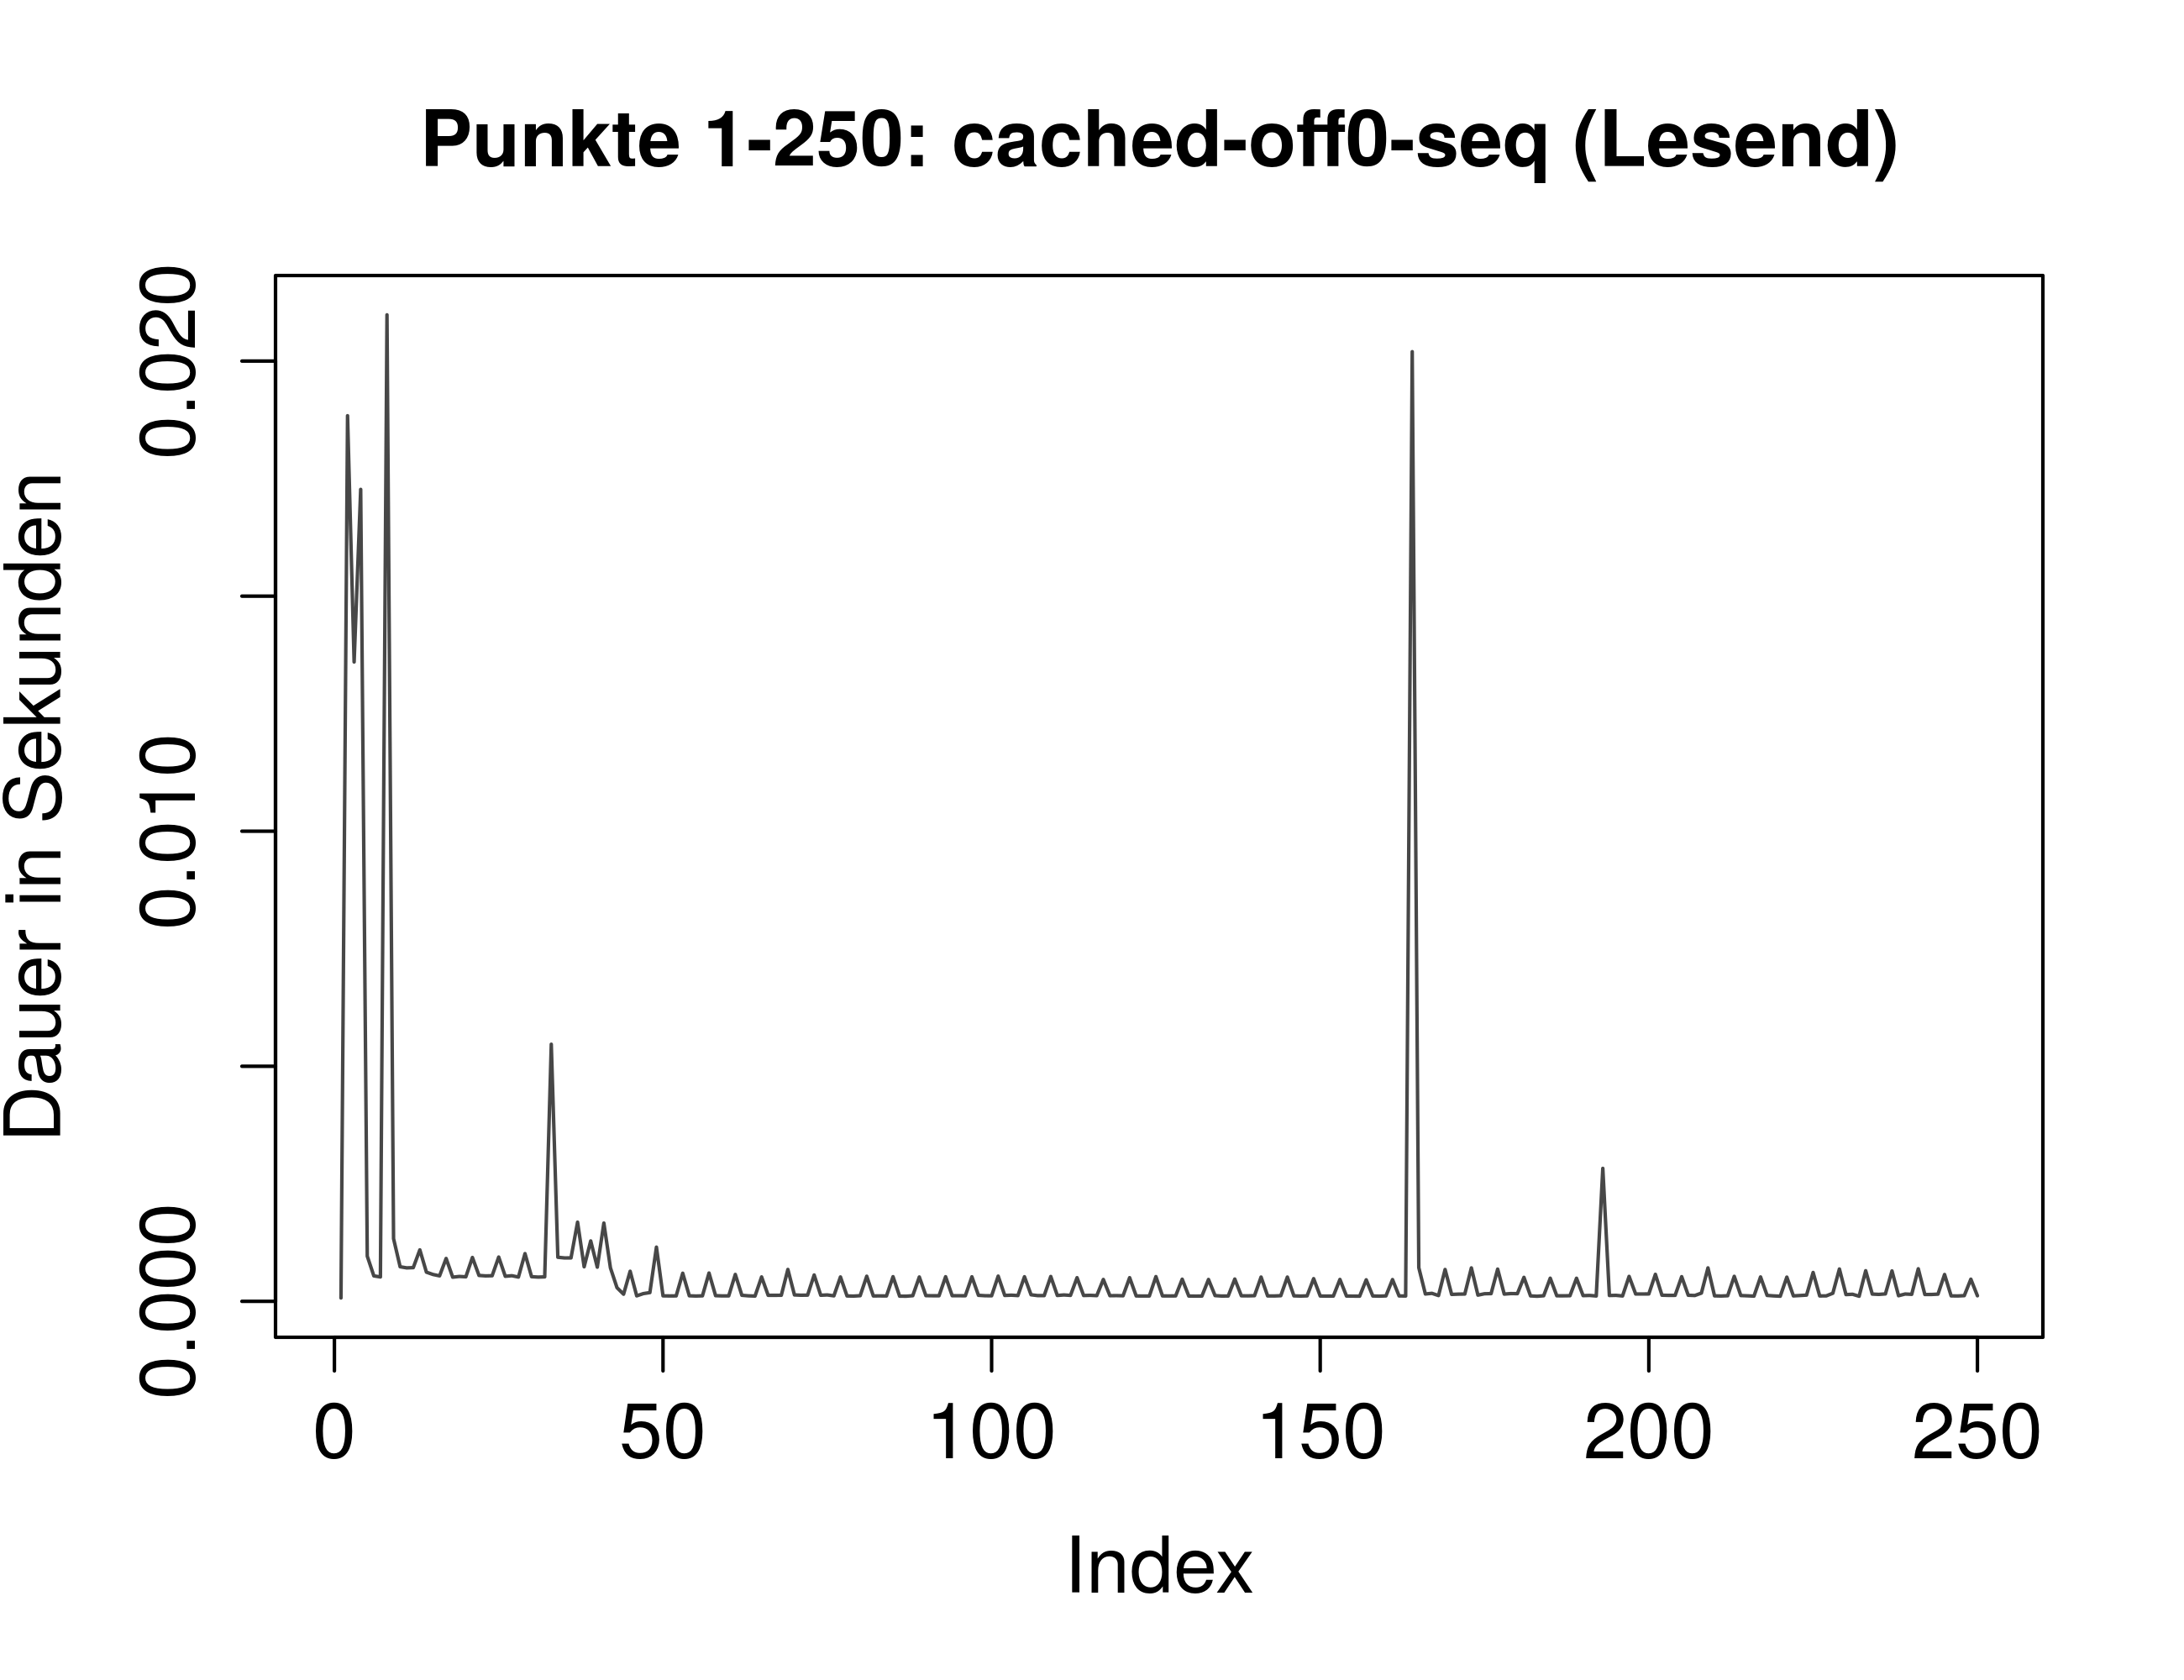
\includegraphics[width=.43\textwidth]{Bilder/Plots/exploration/plot_First250_read_seq.png}
	}
	\hfill
	\subfloat[SEQ-W]{
		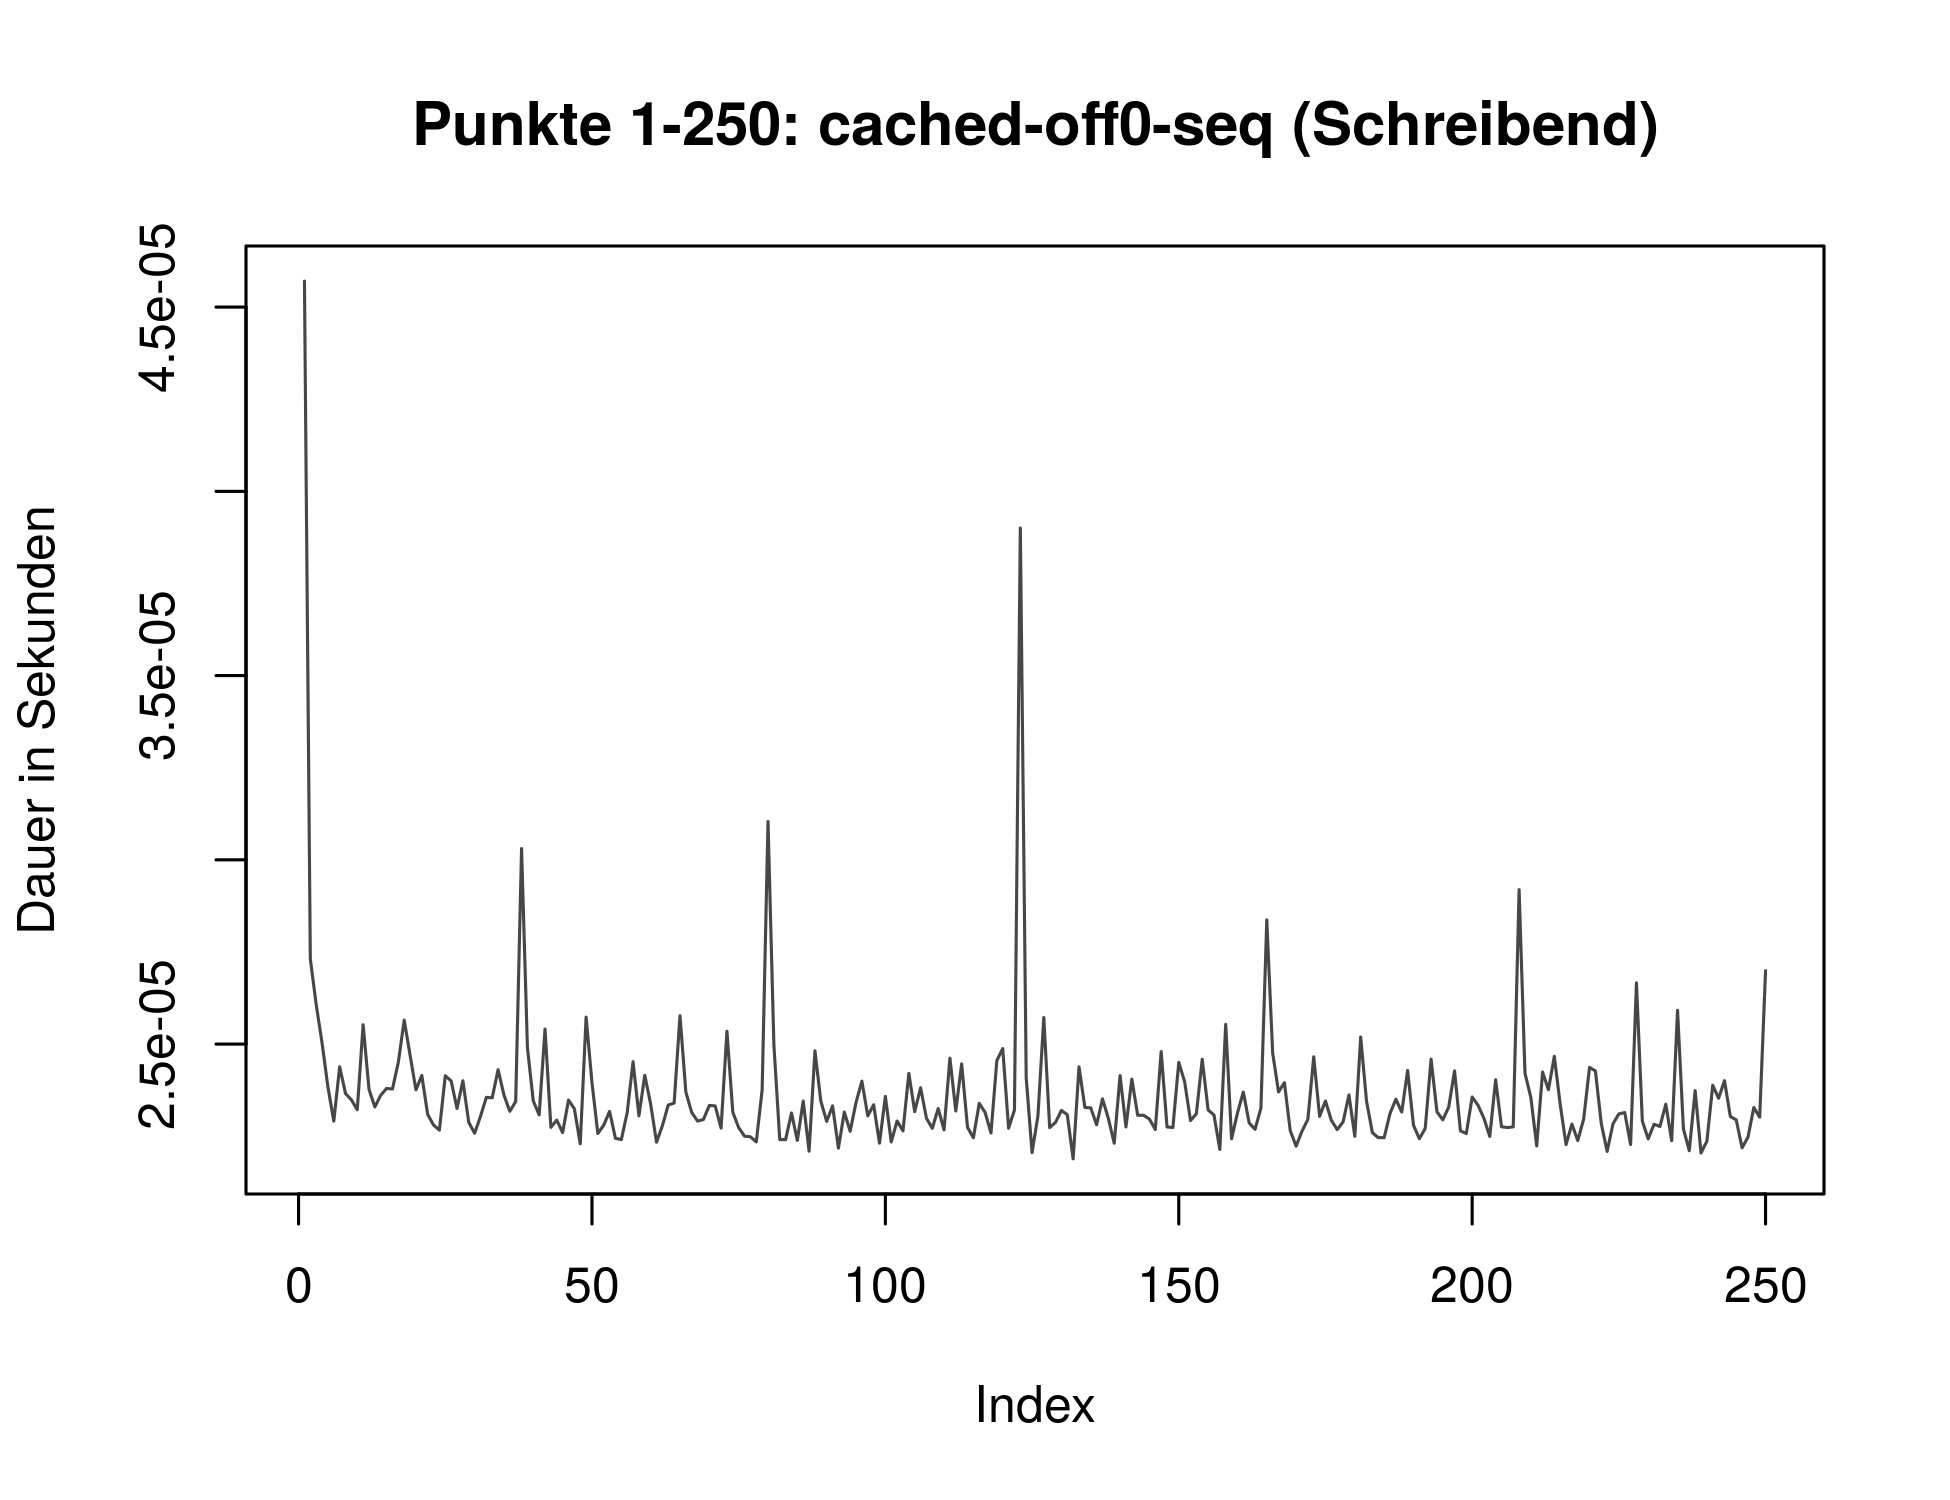
\includegraphics[width=.43\textwidth]{Bilder/Plots/exploration/plot_First250_write_seq.png}
	}\\
	\subfloat[RND-R]{
		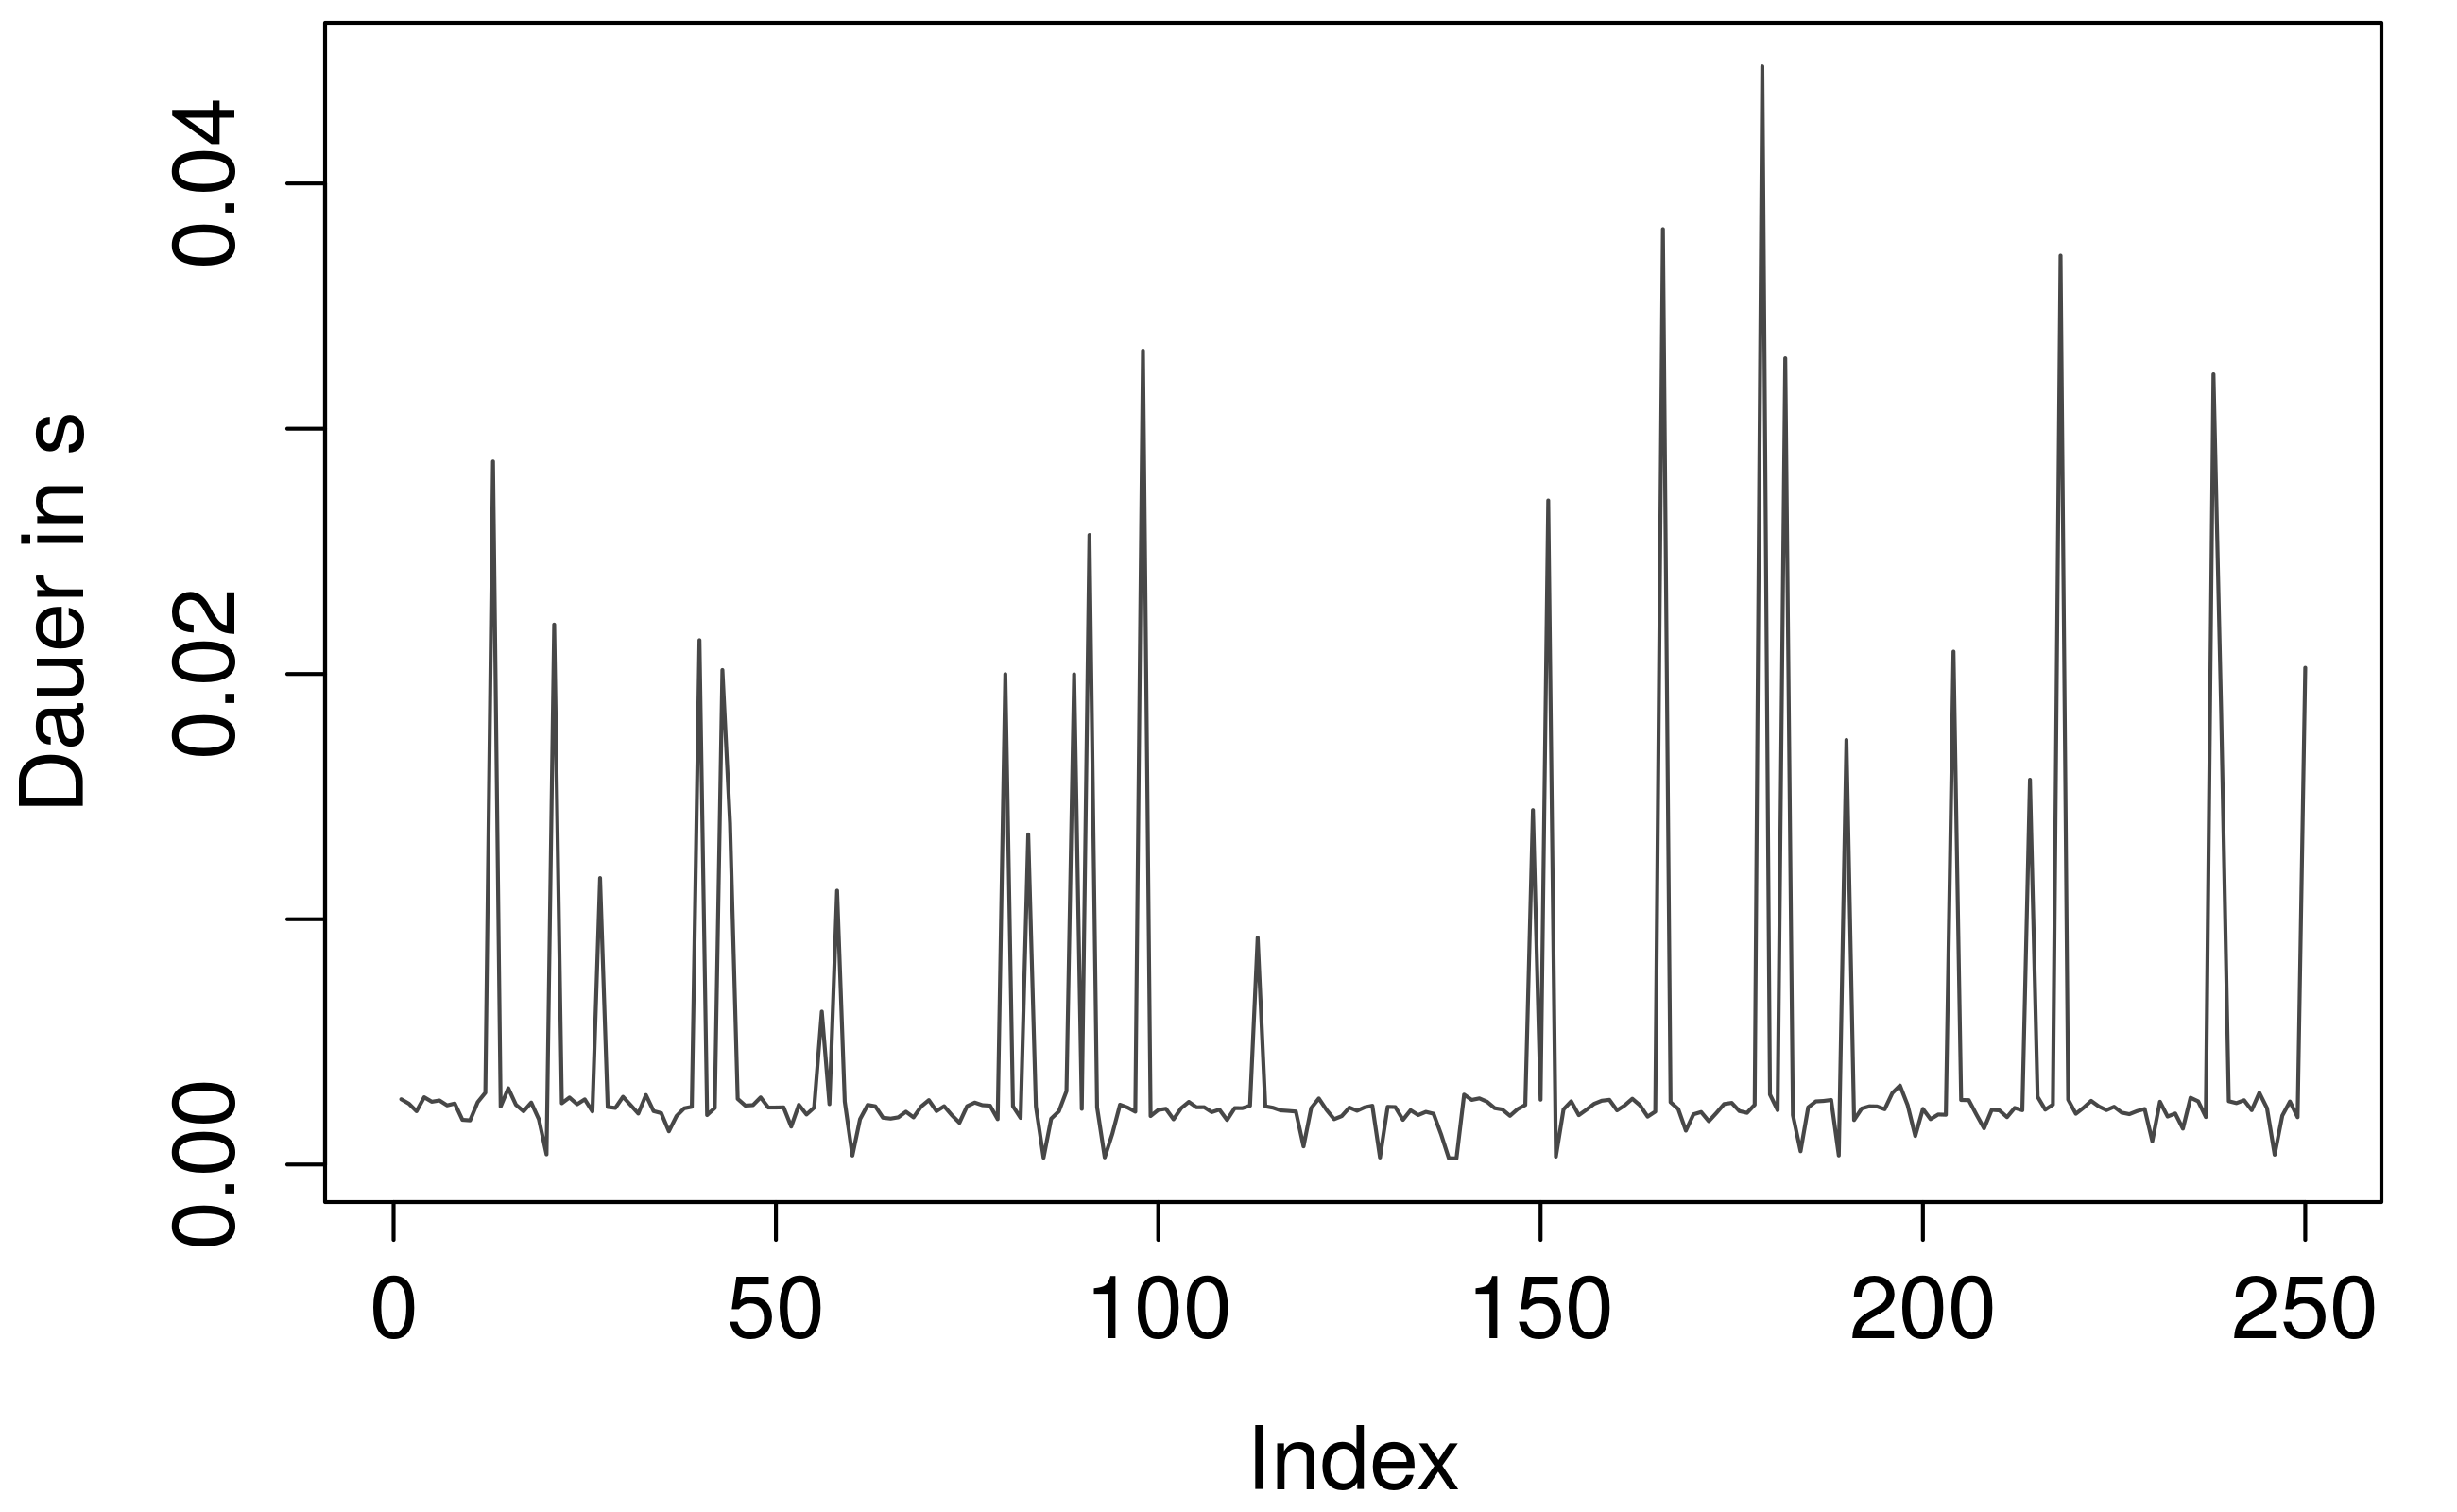
\includegraphics[width=.43\textwidth]{Bilder/Plots/exploration/plot_First250_read_rnd.png}
	}
	\hfill
	\subfloat[RND-W]{
		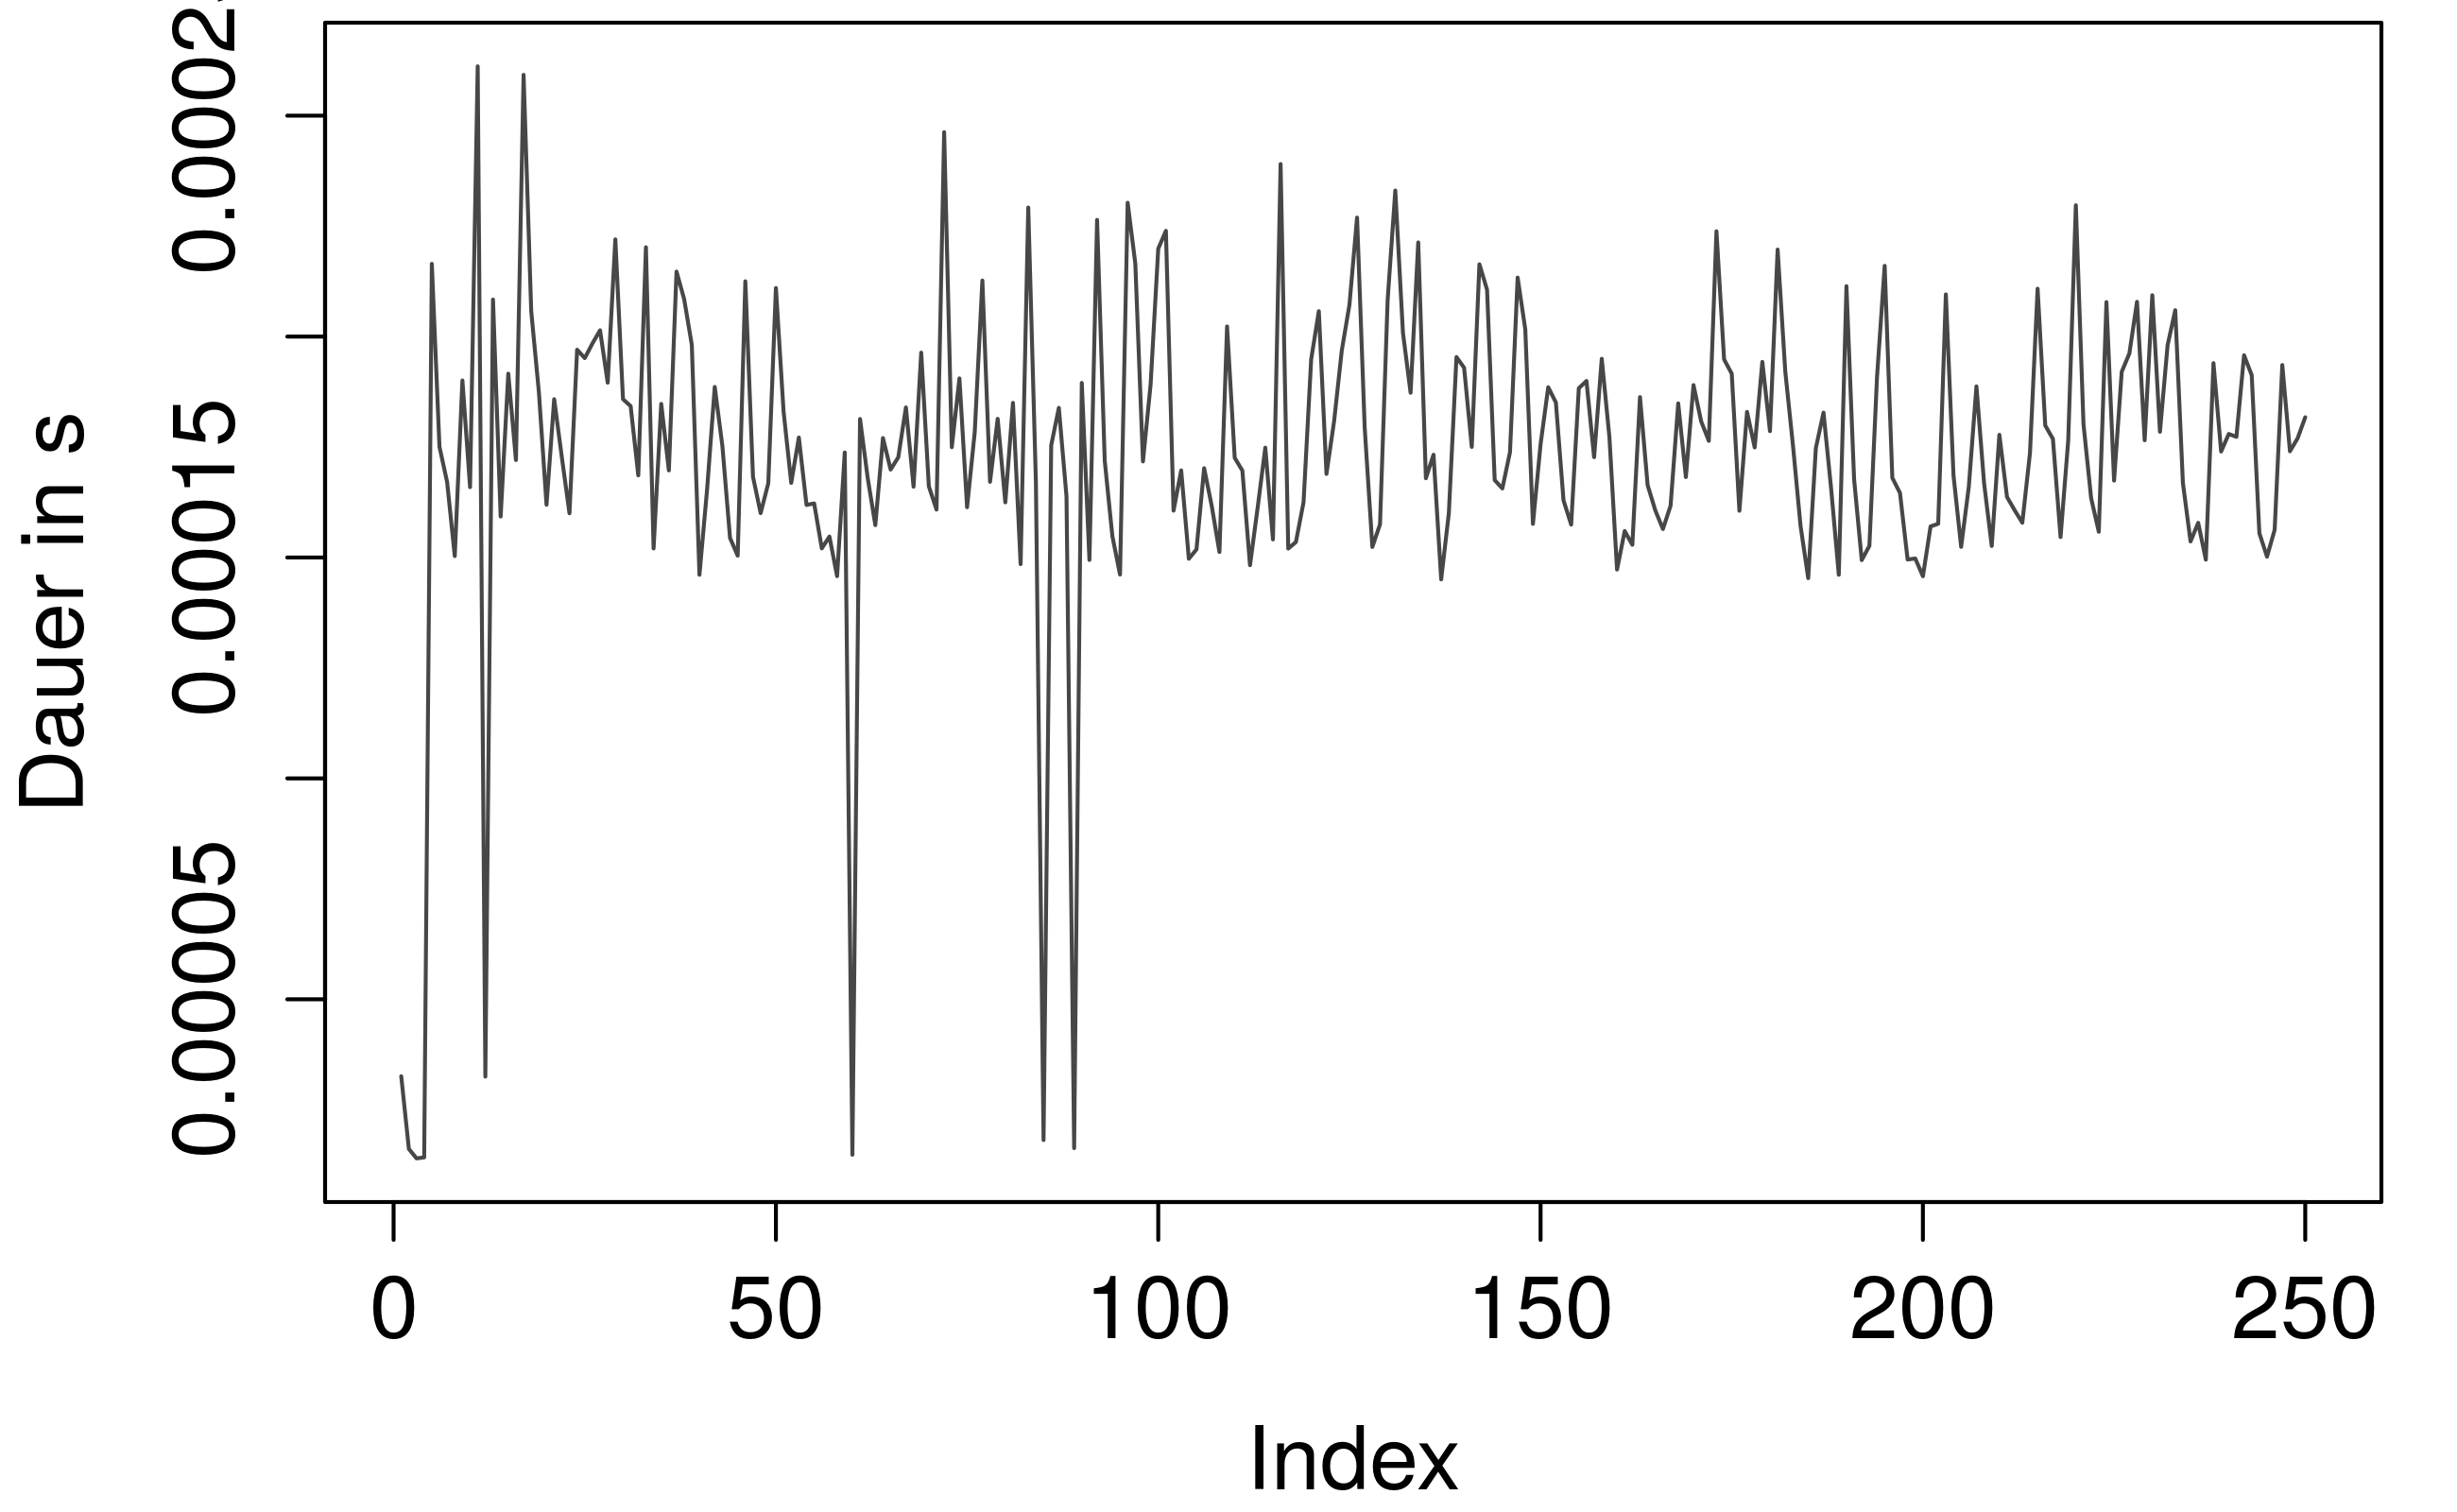
\includegraphics[width=.43\textwidth]{Bilder/Plots/exploration/plot_First250_write_rnd.png}
	}		
	\caption{Detailbetrachtung der ersten 250 Messungen}
	\label{fig:first250}
\end{figure} 

\begin{figure}
	\begin{center}
		\subfloat{
			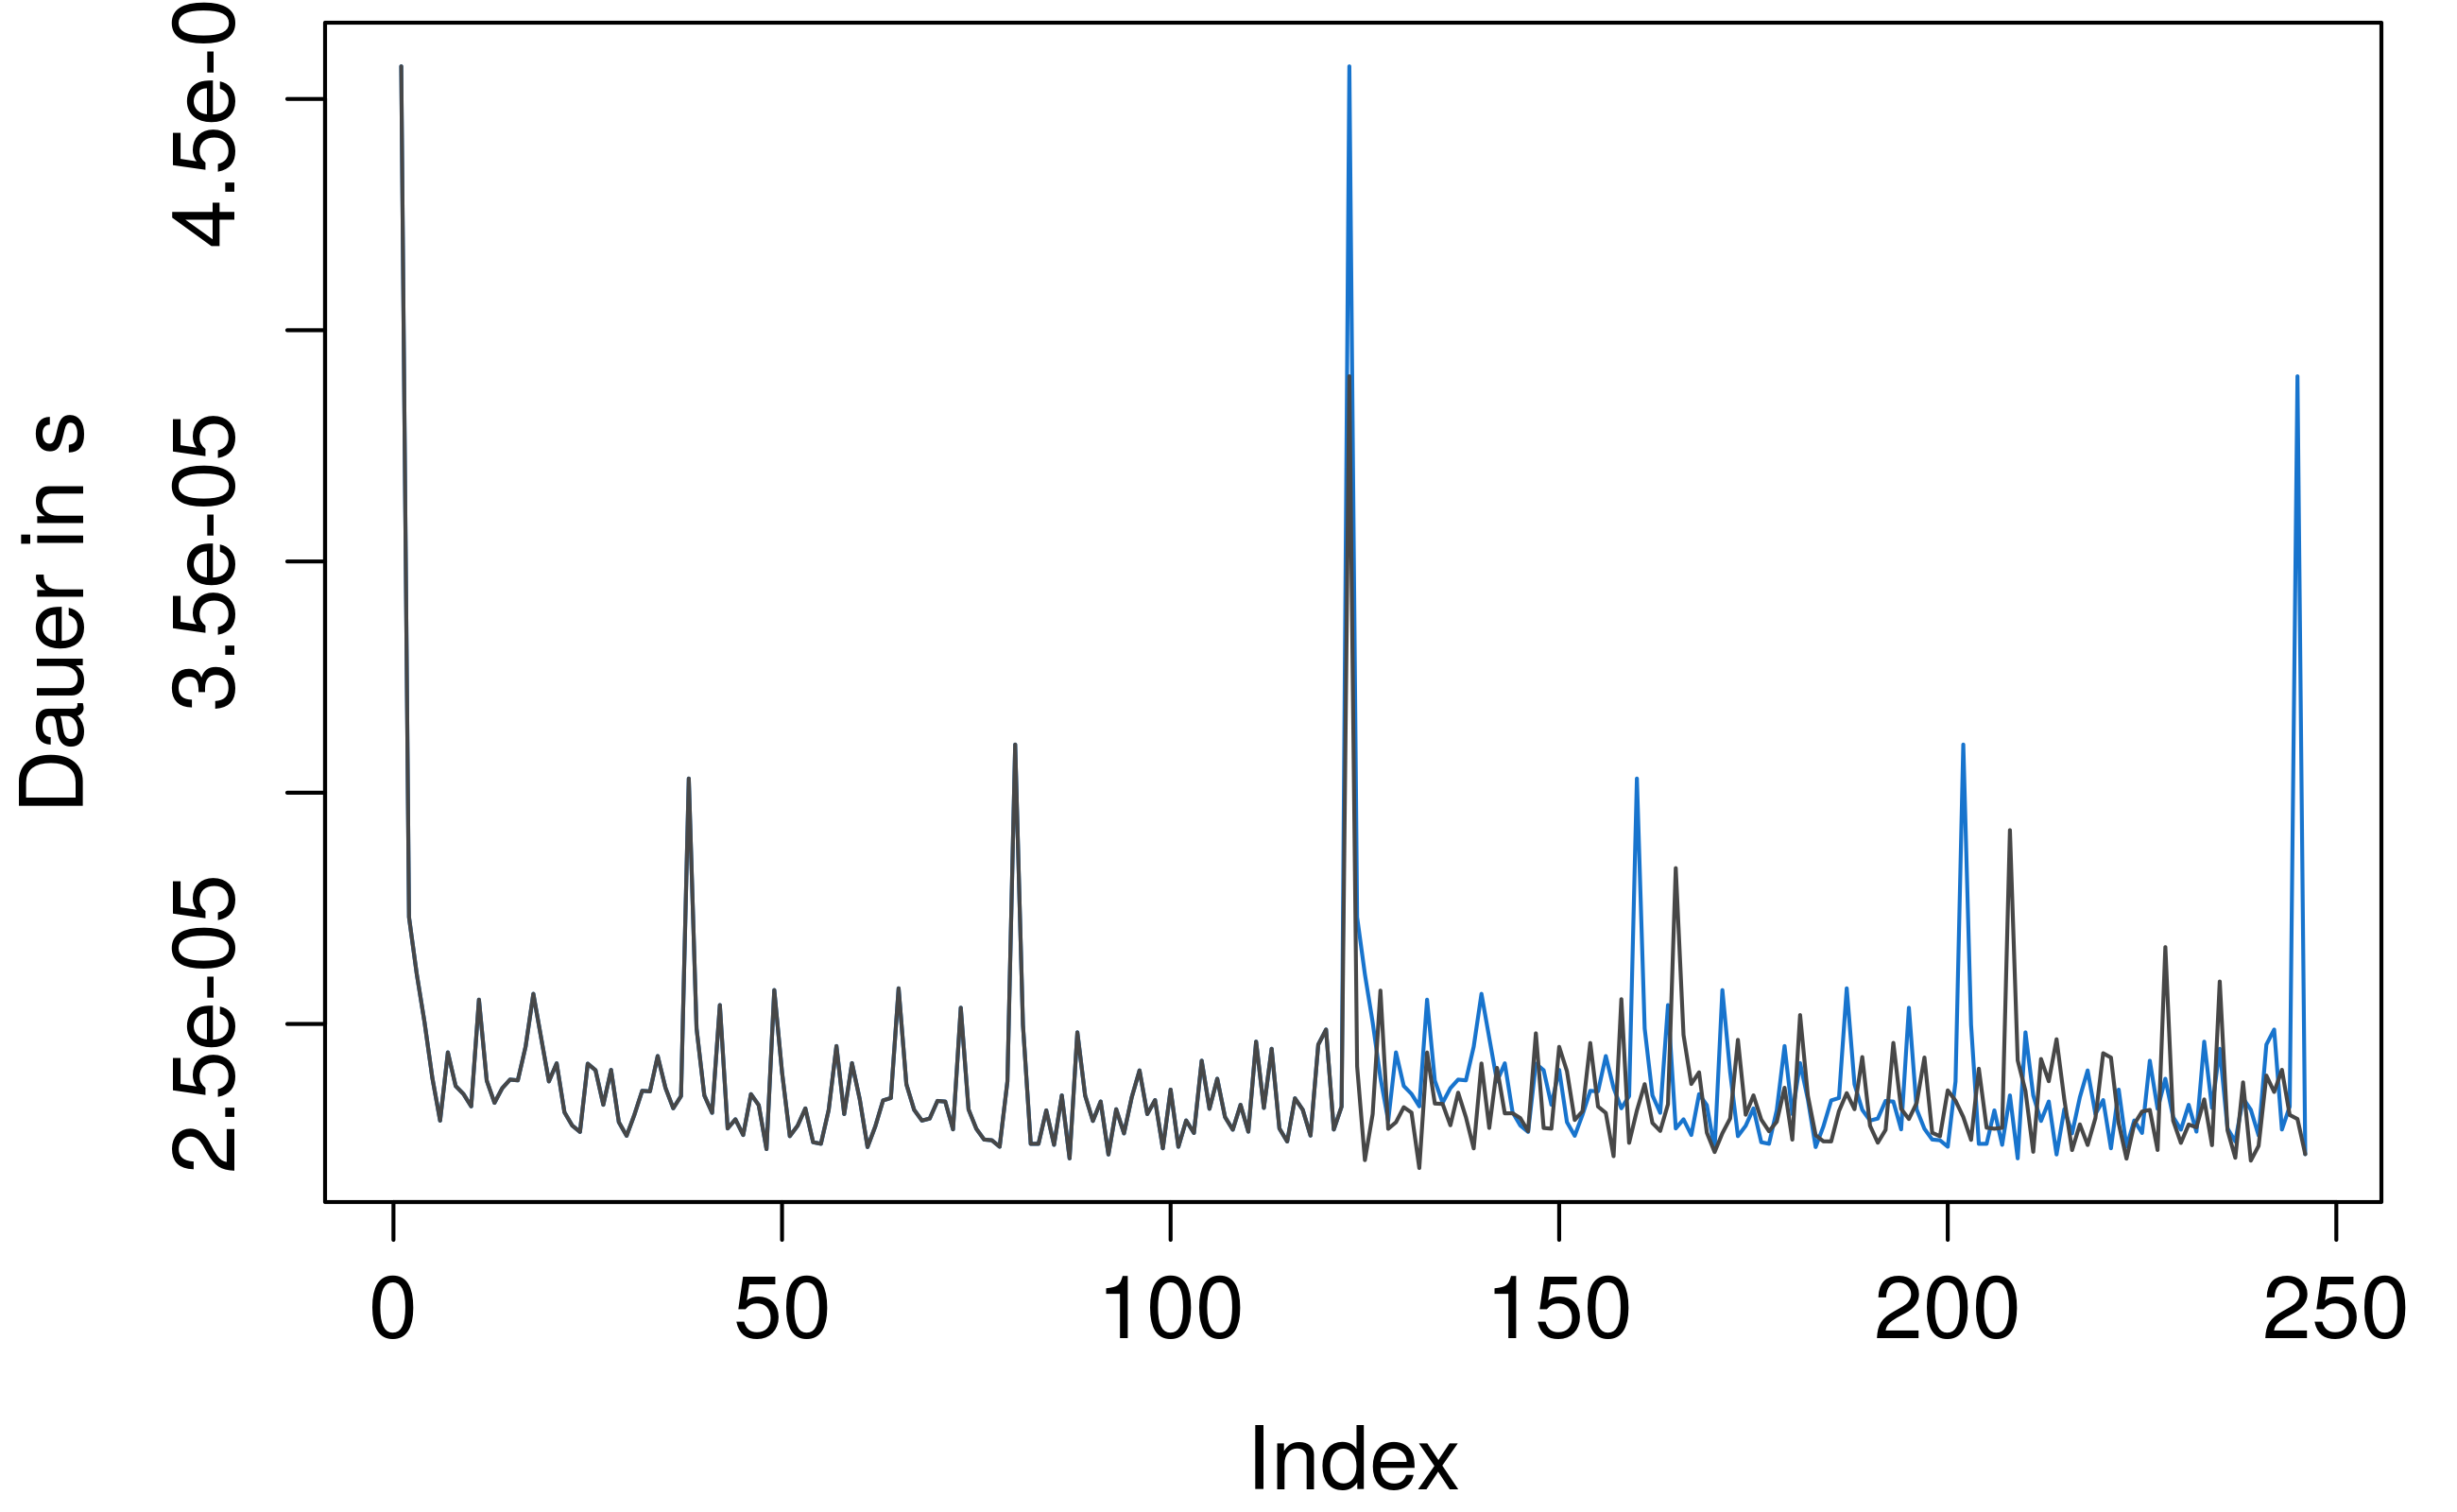
\includegraphics[width=0.6\textwidth]{Bilder/Plots/exploration/plot_periodicitywrite_seq.png}
		}	
		\caption{Ausnutzen des periodischen Verhaltens der Zugriffszeiten als erstes einfaches Modell}
		\label{fig:periodicity}
	\end{center}
\end{figure} 
\medskip

Eine weitere Detailbetrachtung mache ich willkürlich bei den Messungen 100\,001 bis 100\,250.
In diesem Fall scheint eine Periodizität in den Zugriffszeiten zu SEQ-R vorhanden zu sein. In Abbildung \ref{fig:periodicity100001} wurde eine Überlappung von Laufzeit und Vorhersage wie zuvor durchgeführt (diesmal werden die ersten 129 Messungen wiederholt). Man erkennt, dass dieses simple Modell die Ausreißer für diesen kleinen Ausschnitt tatsächlich exakt vorhersagen kann.\\
Im Allgemeinen kann dies jedoch offensichtlich nicht funktionieren.
Doch die Annahme einer gewissen Periodizität in der Leistung des E/A-Systems scheint gerechtfertigt zu sein.
Ein Modell, das versucht diese auszunutzen muss dabei eine komplexere Methode als schlichtes Übertragen vorheriger Leistungswerte ausnutzen, ansonsten kann es wohl nur in äußerst eingeschränktem Maße korrekte Leistung vorhersagen.

\begin{figure}
	\centering
	\subfloat[SEQ-R]{
		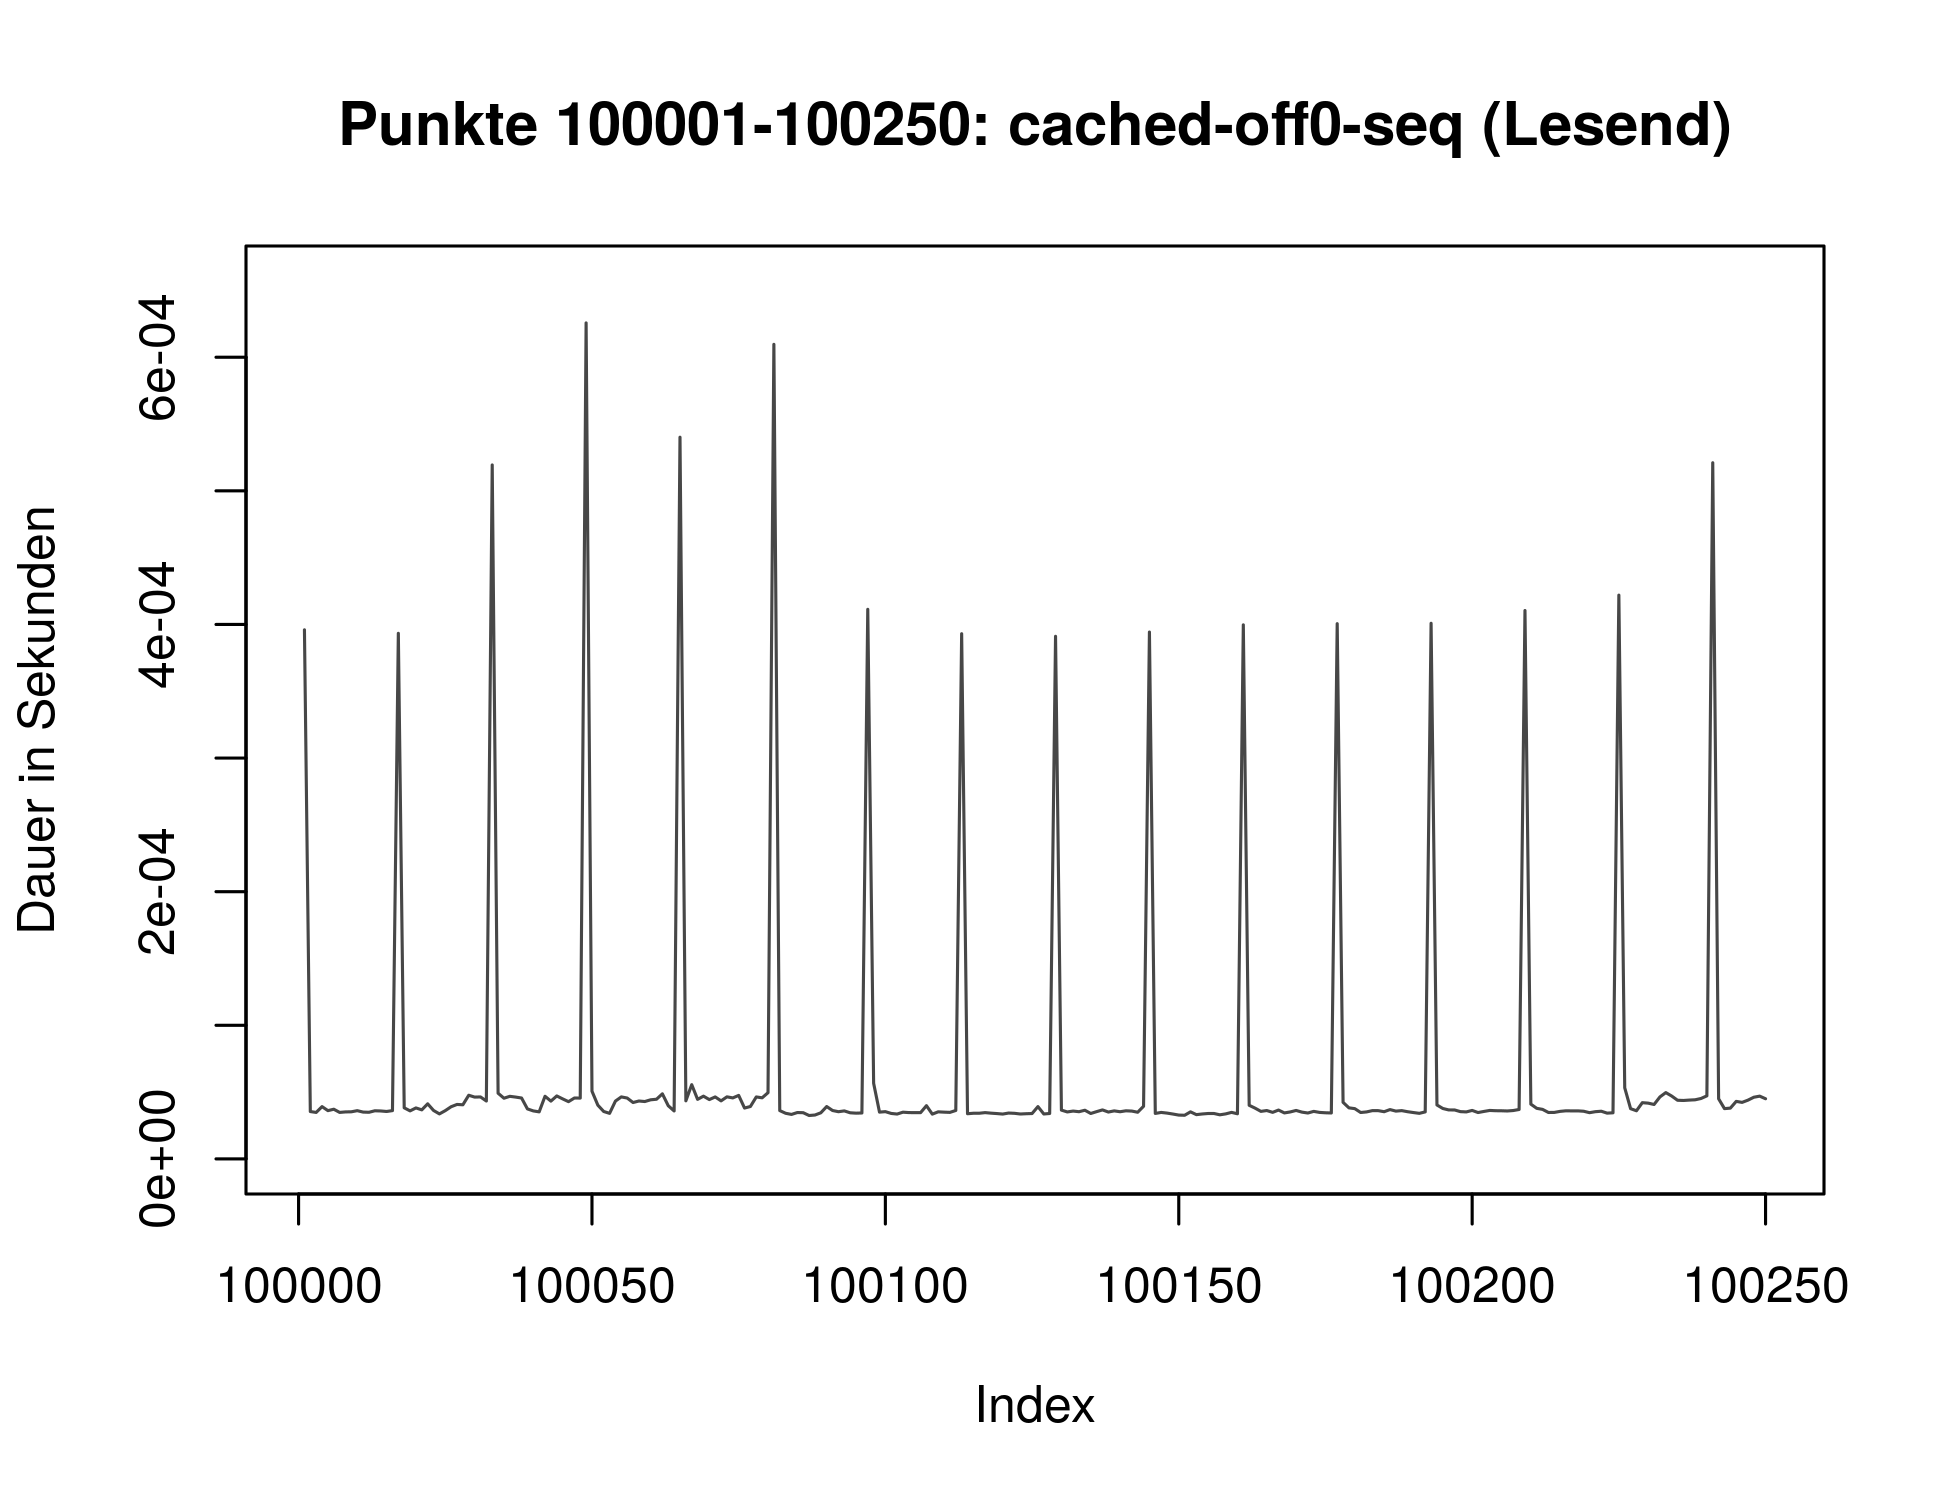
\includegraphics[width=.43\textwidth]{Bilder/Plots/exploration/plot_From100001to100250_read_seq.png}
	}
	\hfill
	\subfloat[SEQ-W]{
		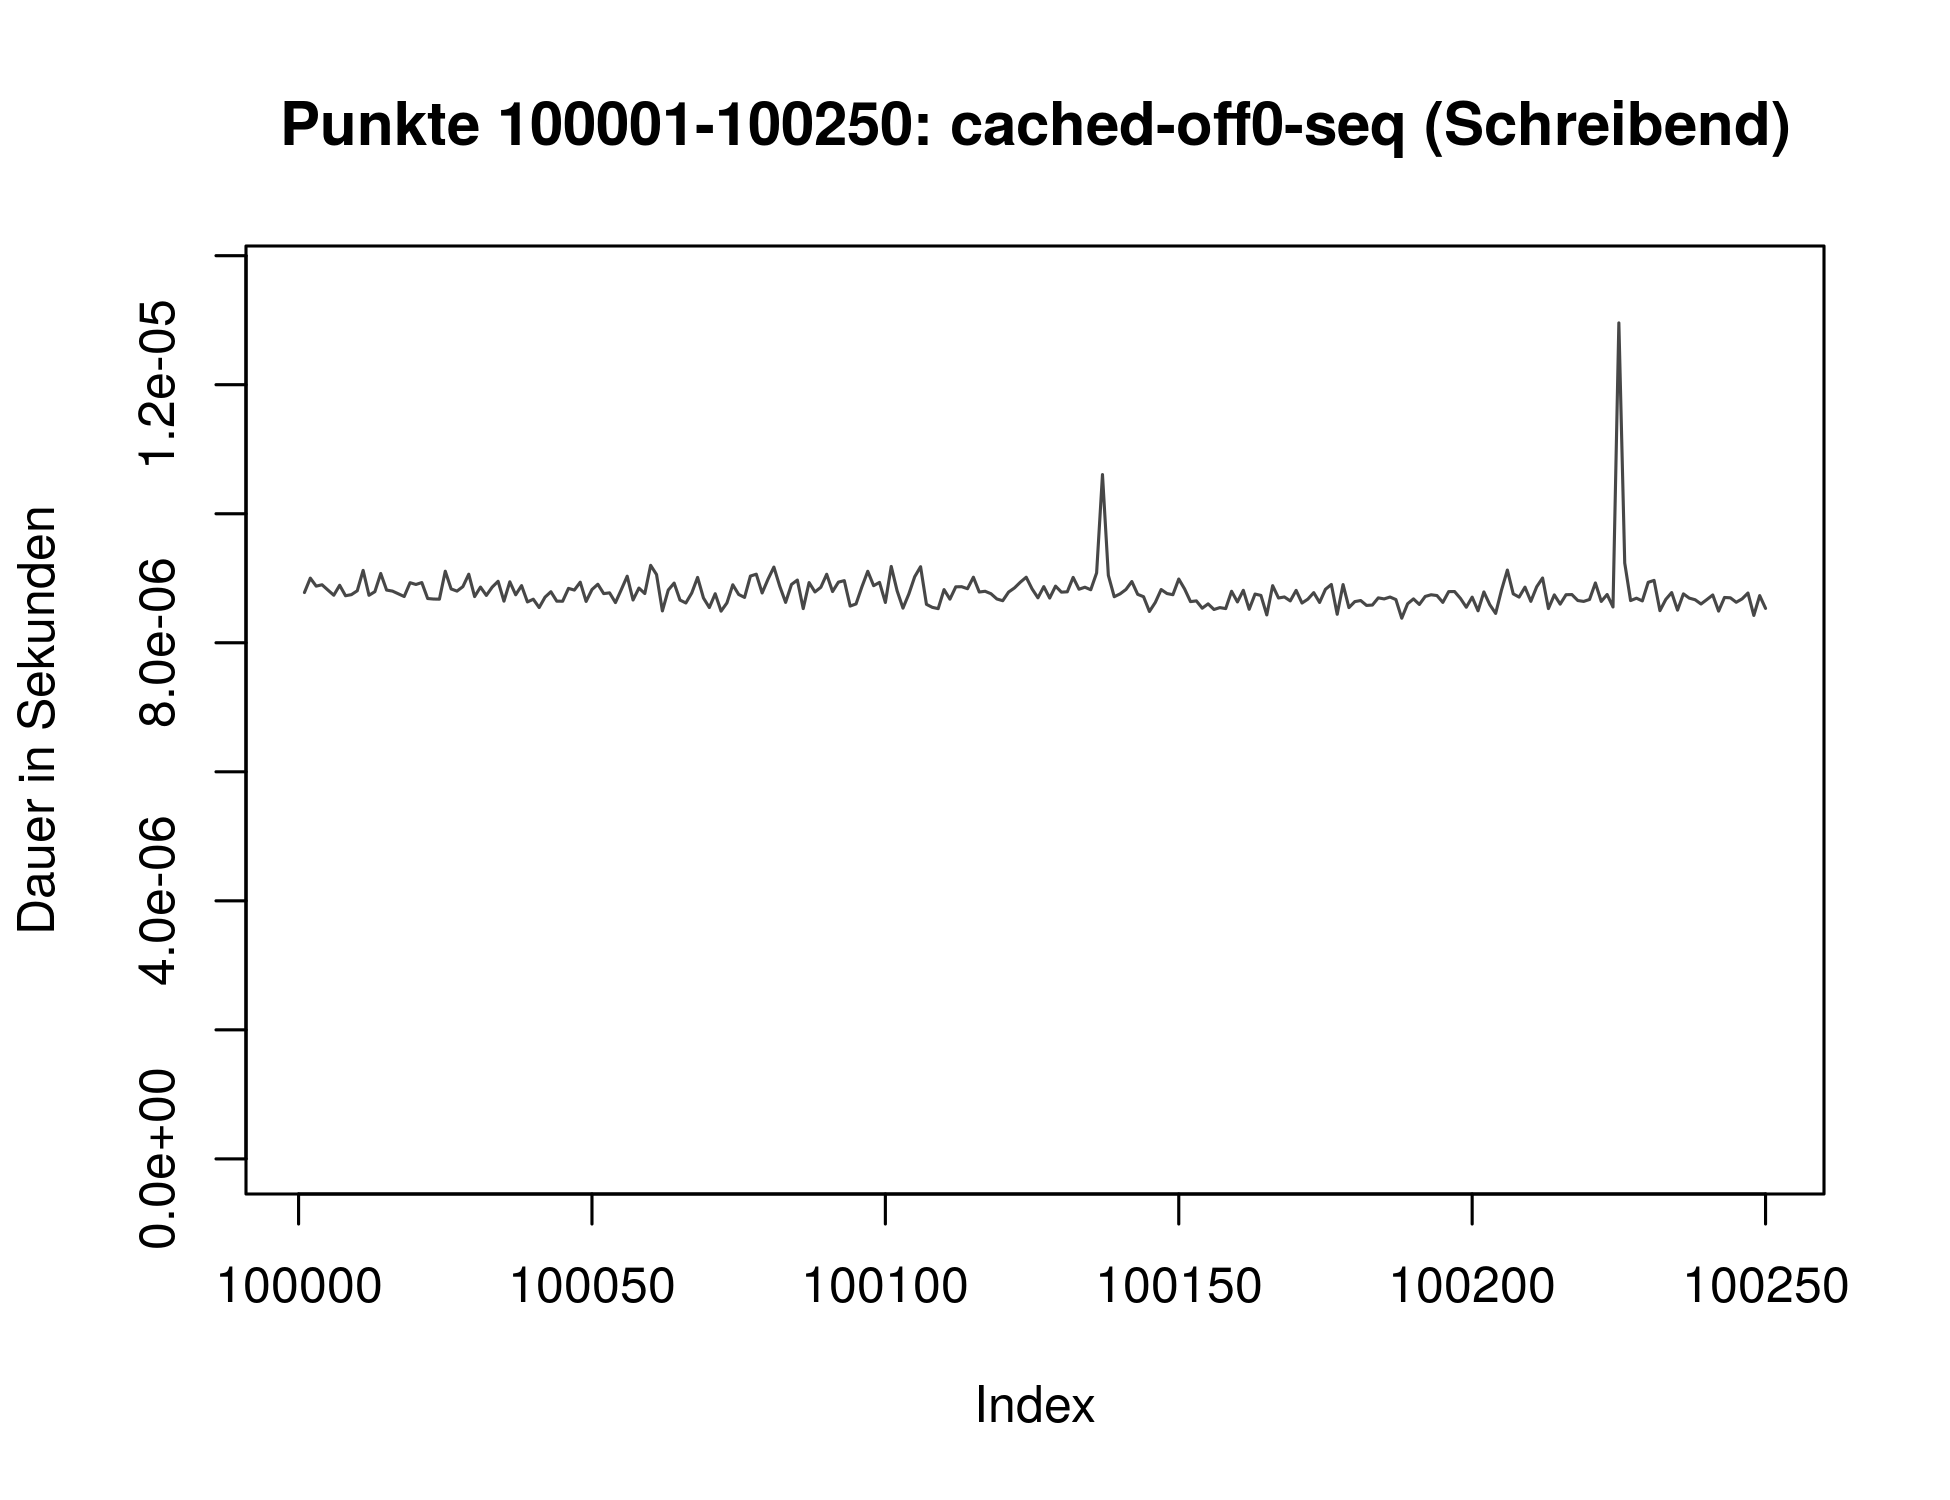
\includegraphics[width=.43\textwidth]{Bilder/Plots/exploration/plot_From100001to100250_write_seq.png}
	}\\
	\subfloat[RND-R]{
		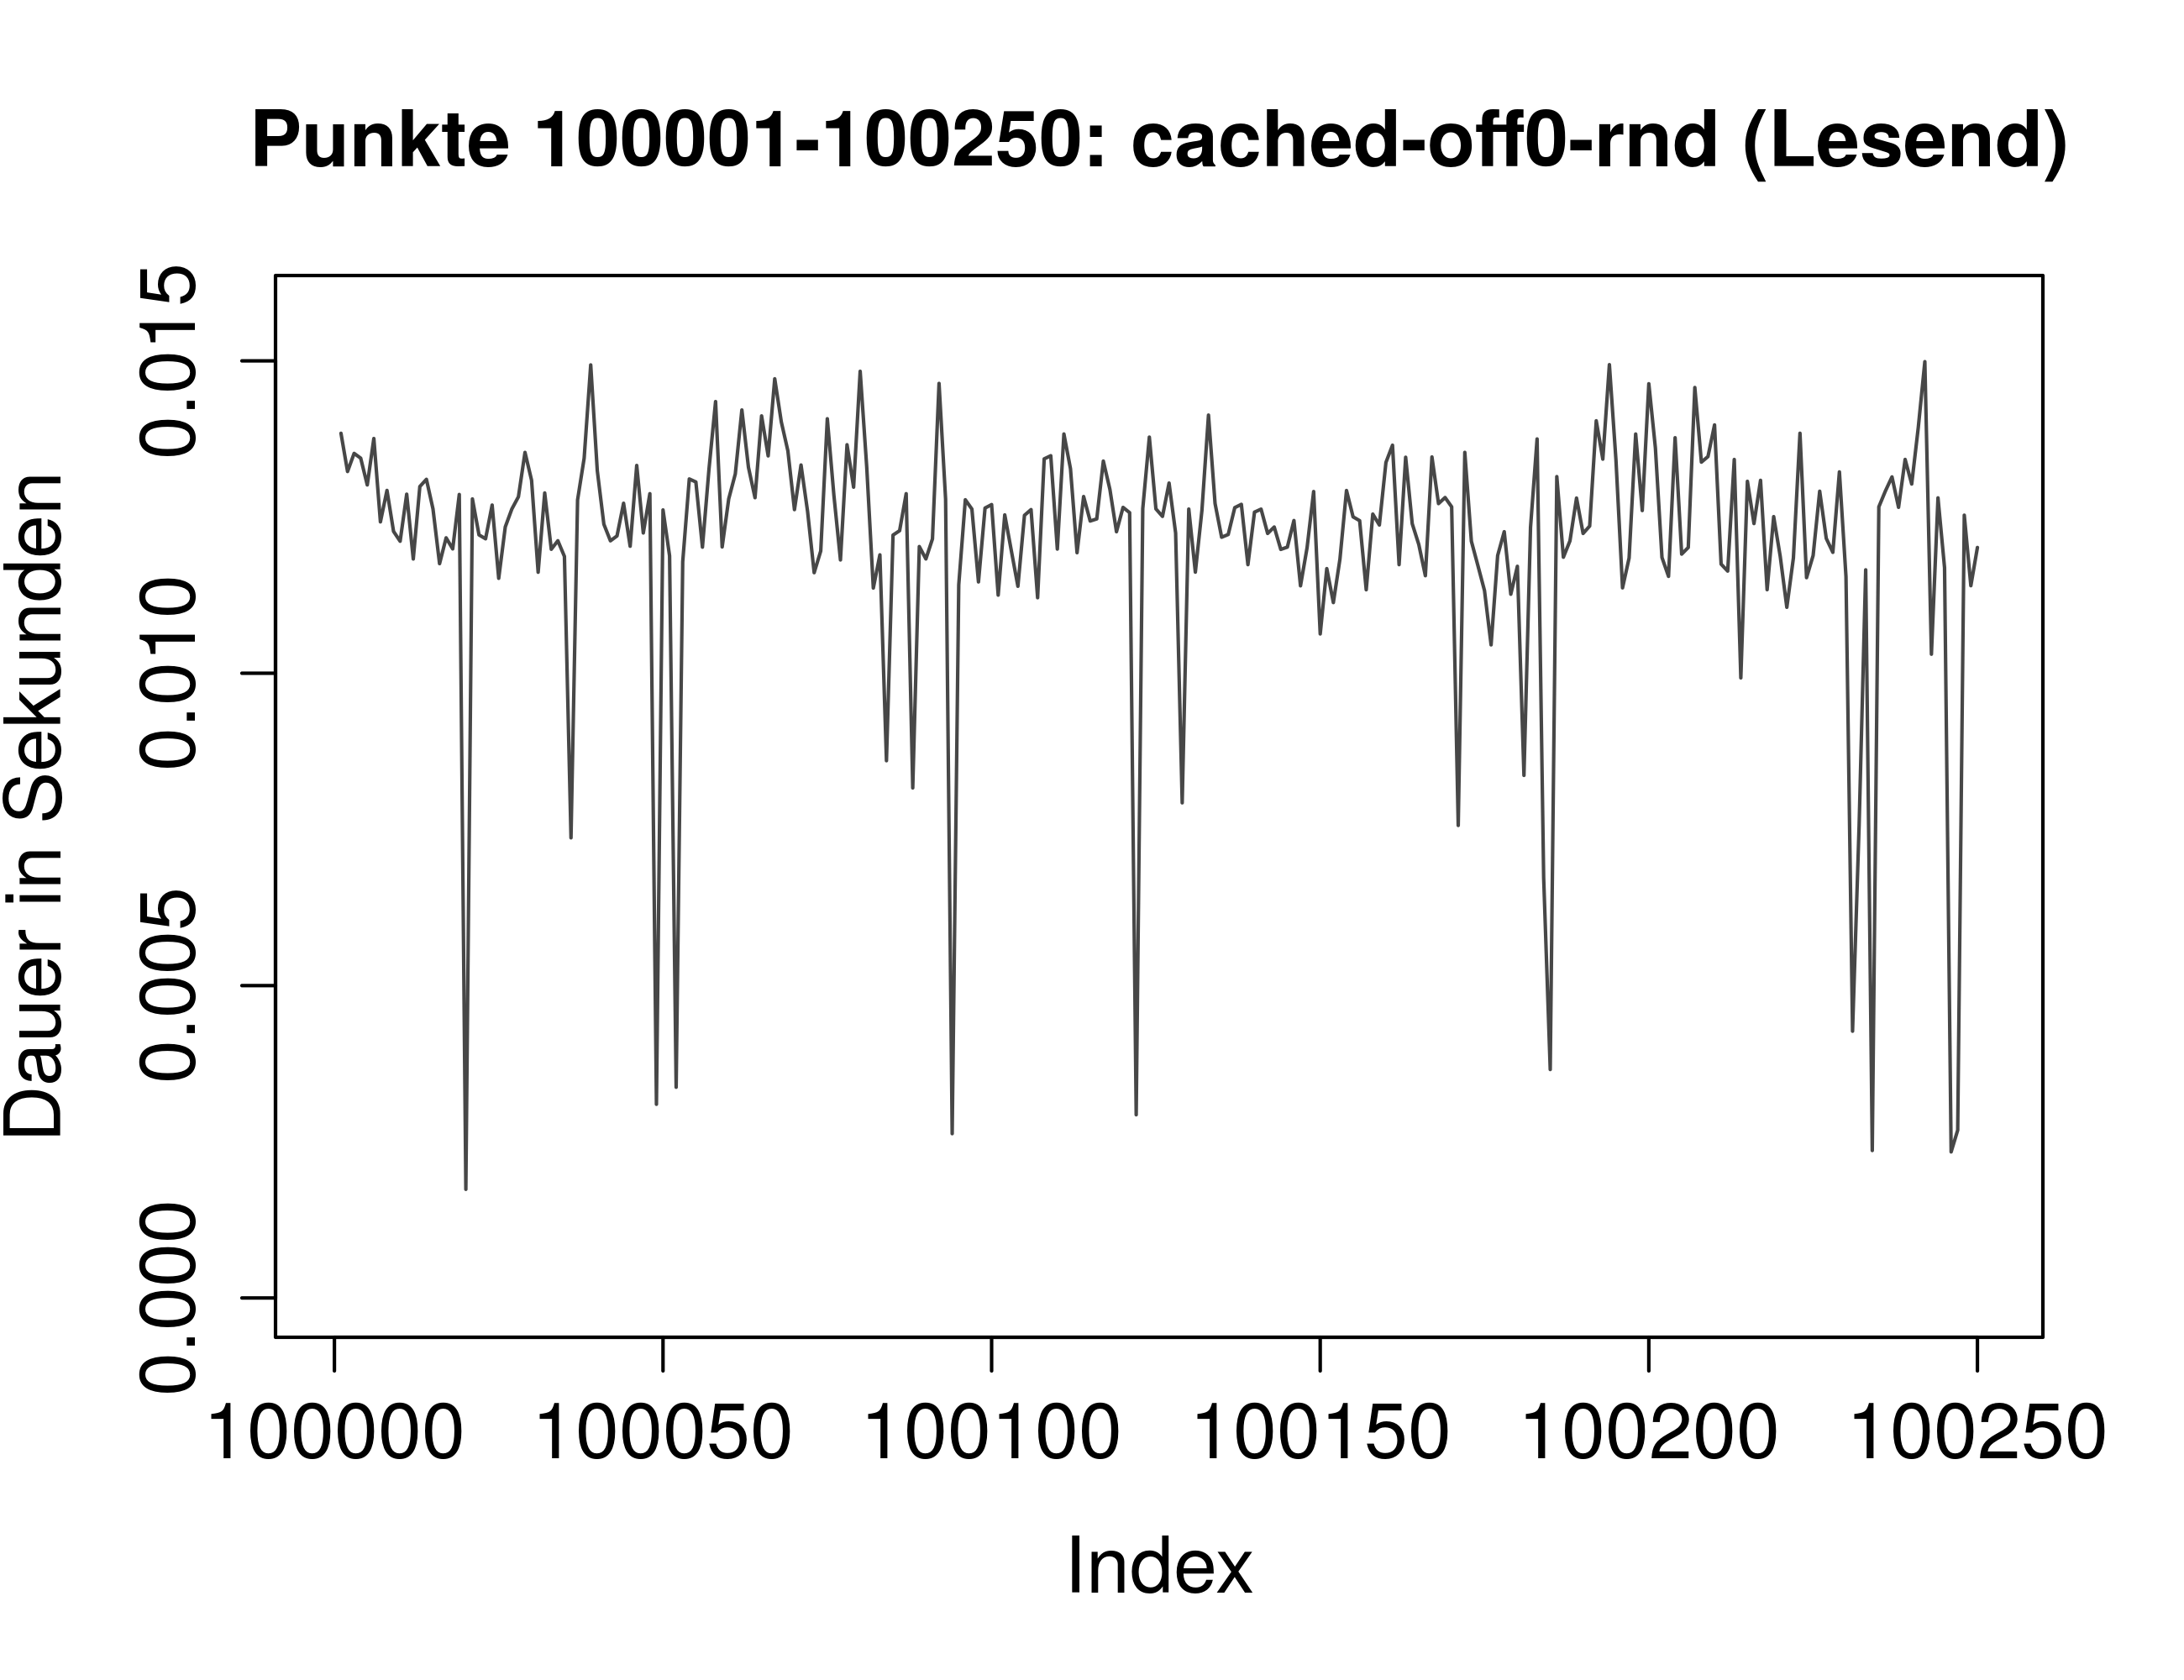
\includegraphics[width=.43\textwidth]{Bilder/Plots/exploration/plot_From100001to100250_read_rnd.png}
	}
	\hfill
	\subfloat[RND-W]{
		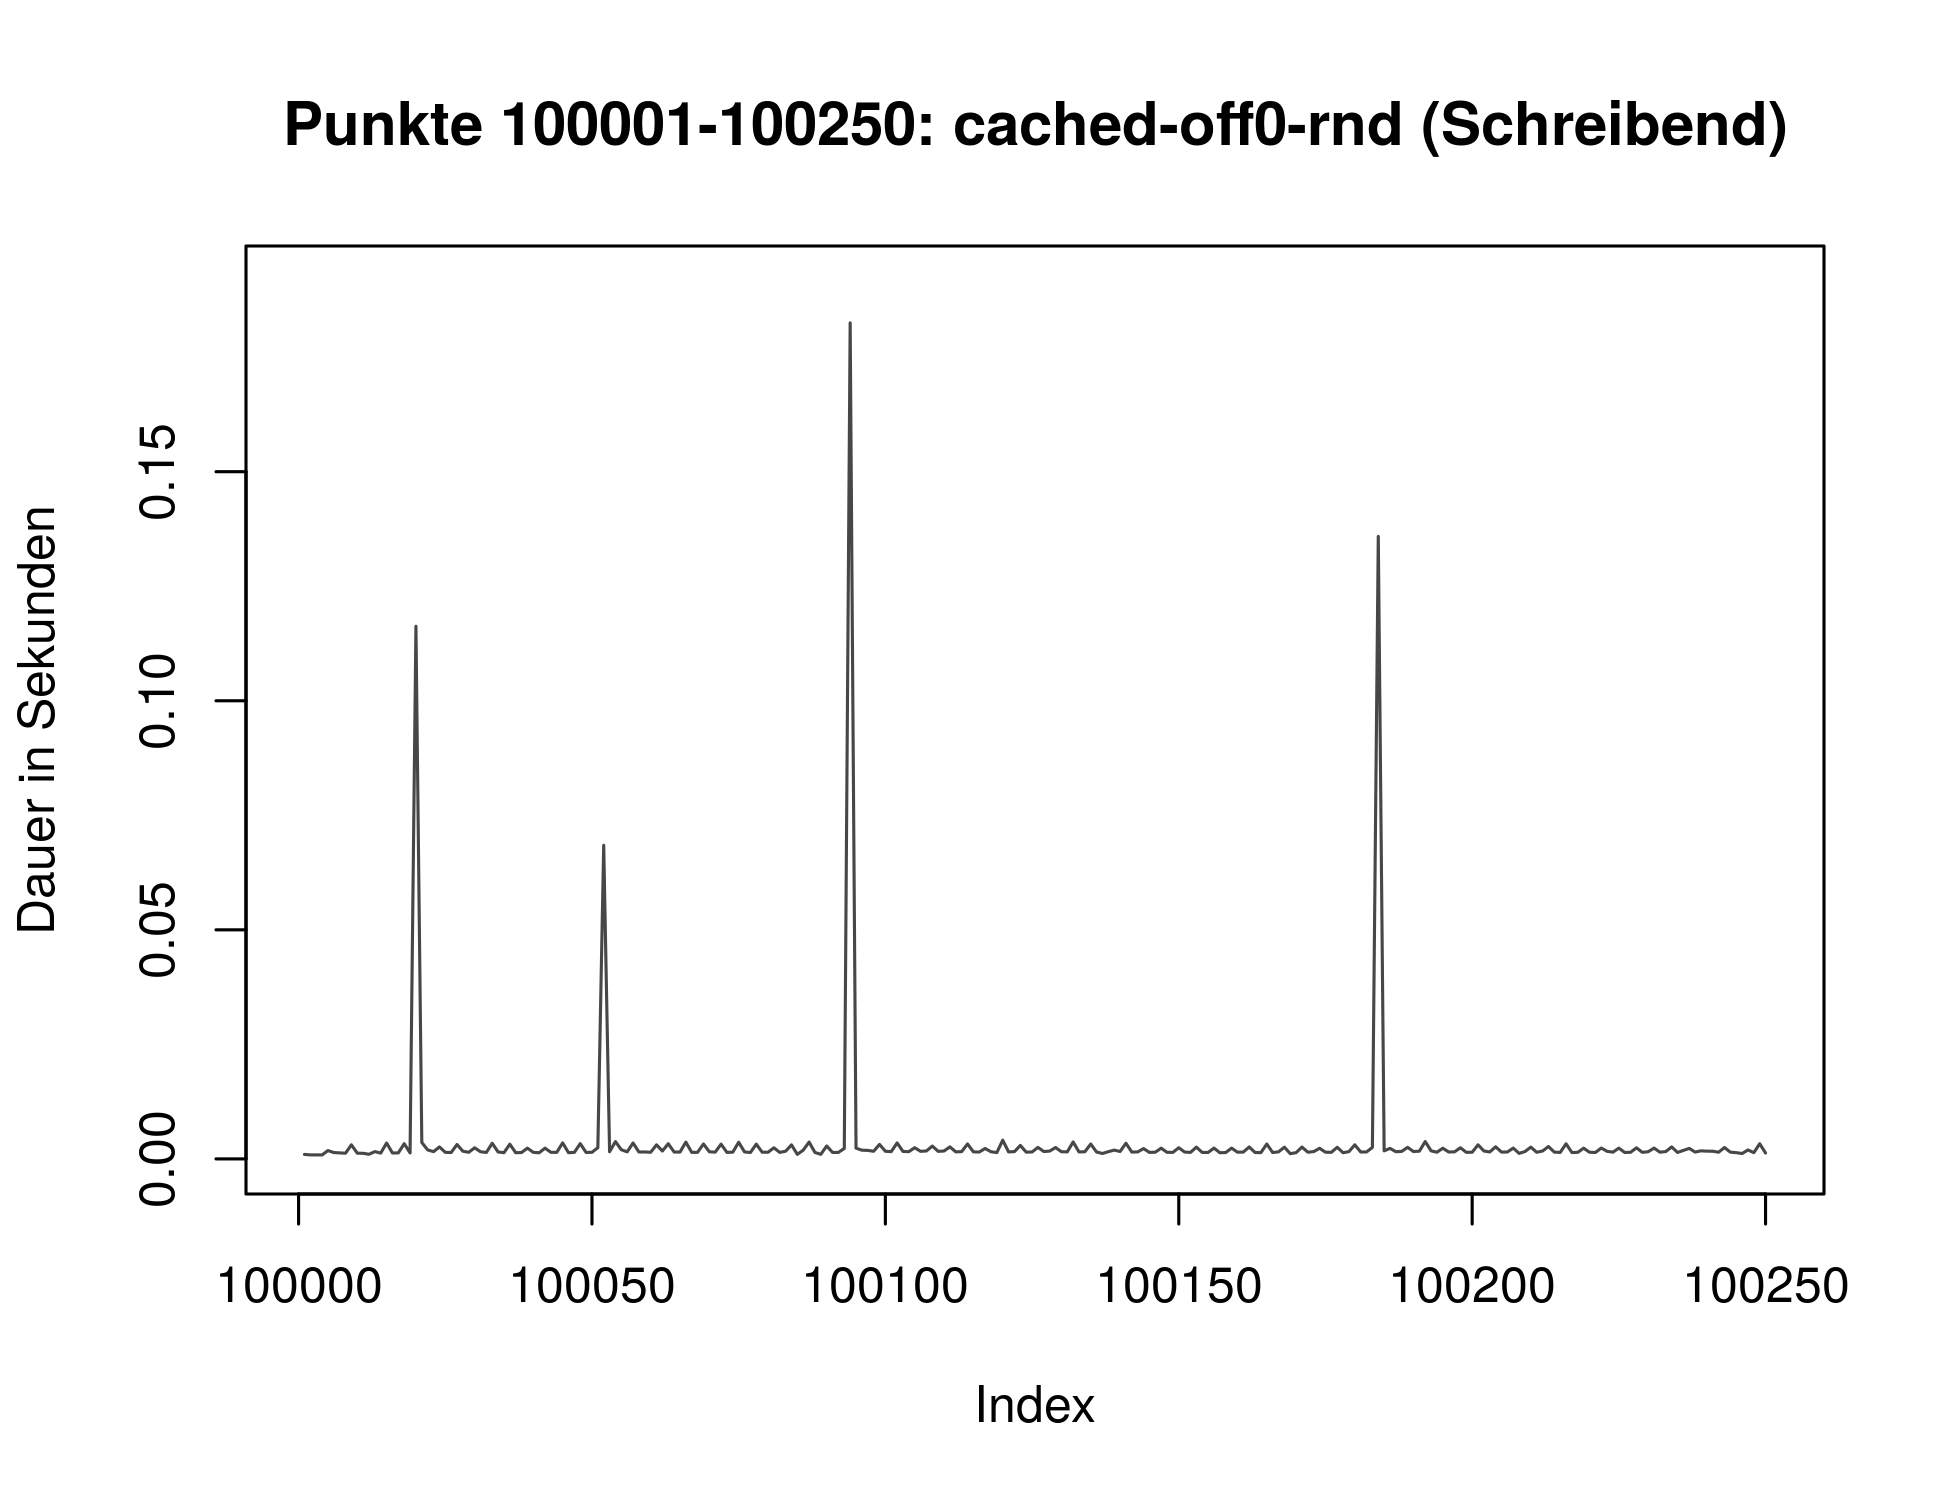
\includegraphics[width=.43\textwidth]{Bilder/Plots/exploration/plot_From100001to100250_write_rnd.png}
	}		
	\caption{Detailbetrachtung der Messungen 100\,001 bis 100\,250}
	\label{fig:from100001}
\end{figure} 

\begin{figure}
	\begin{center}
		\subfloat{
			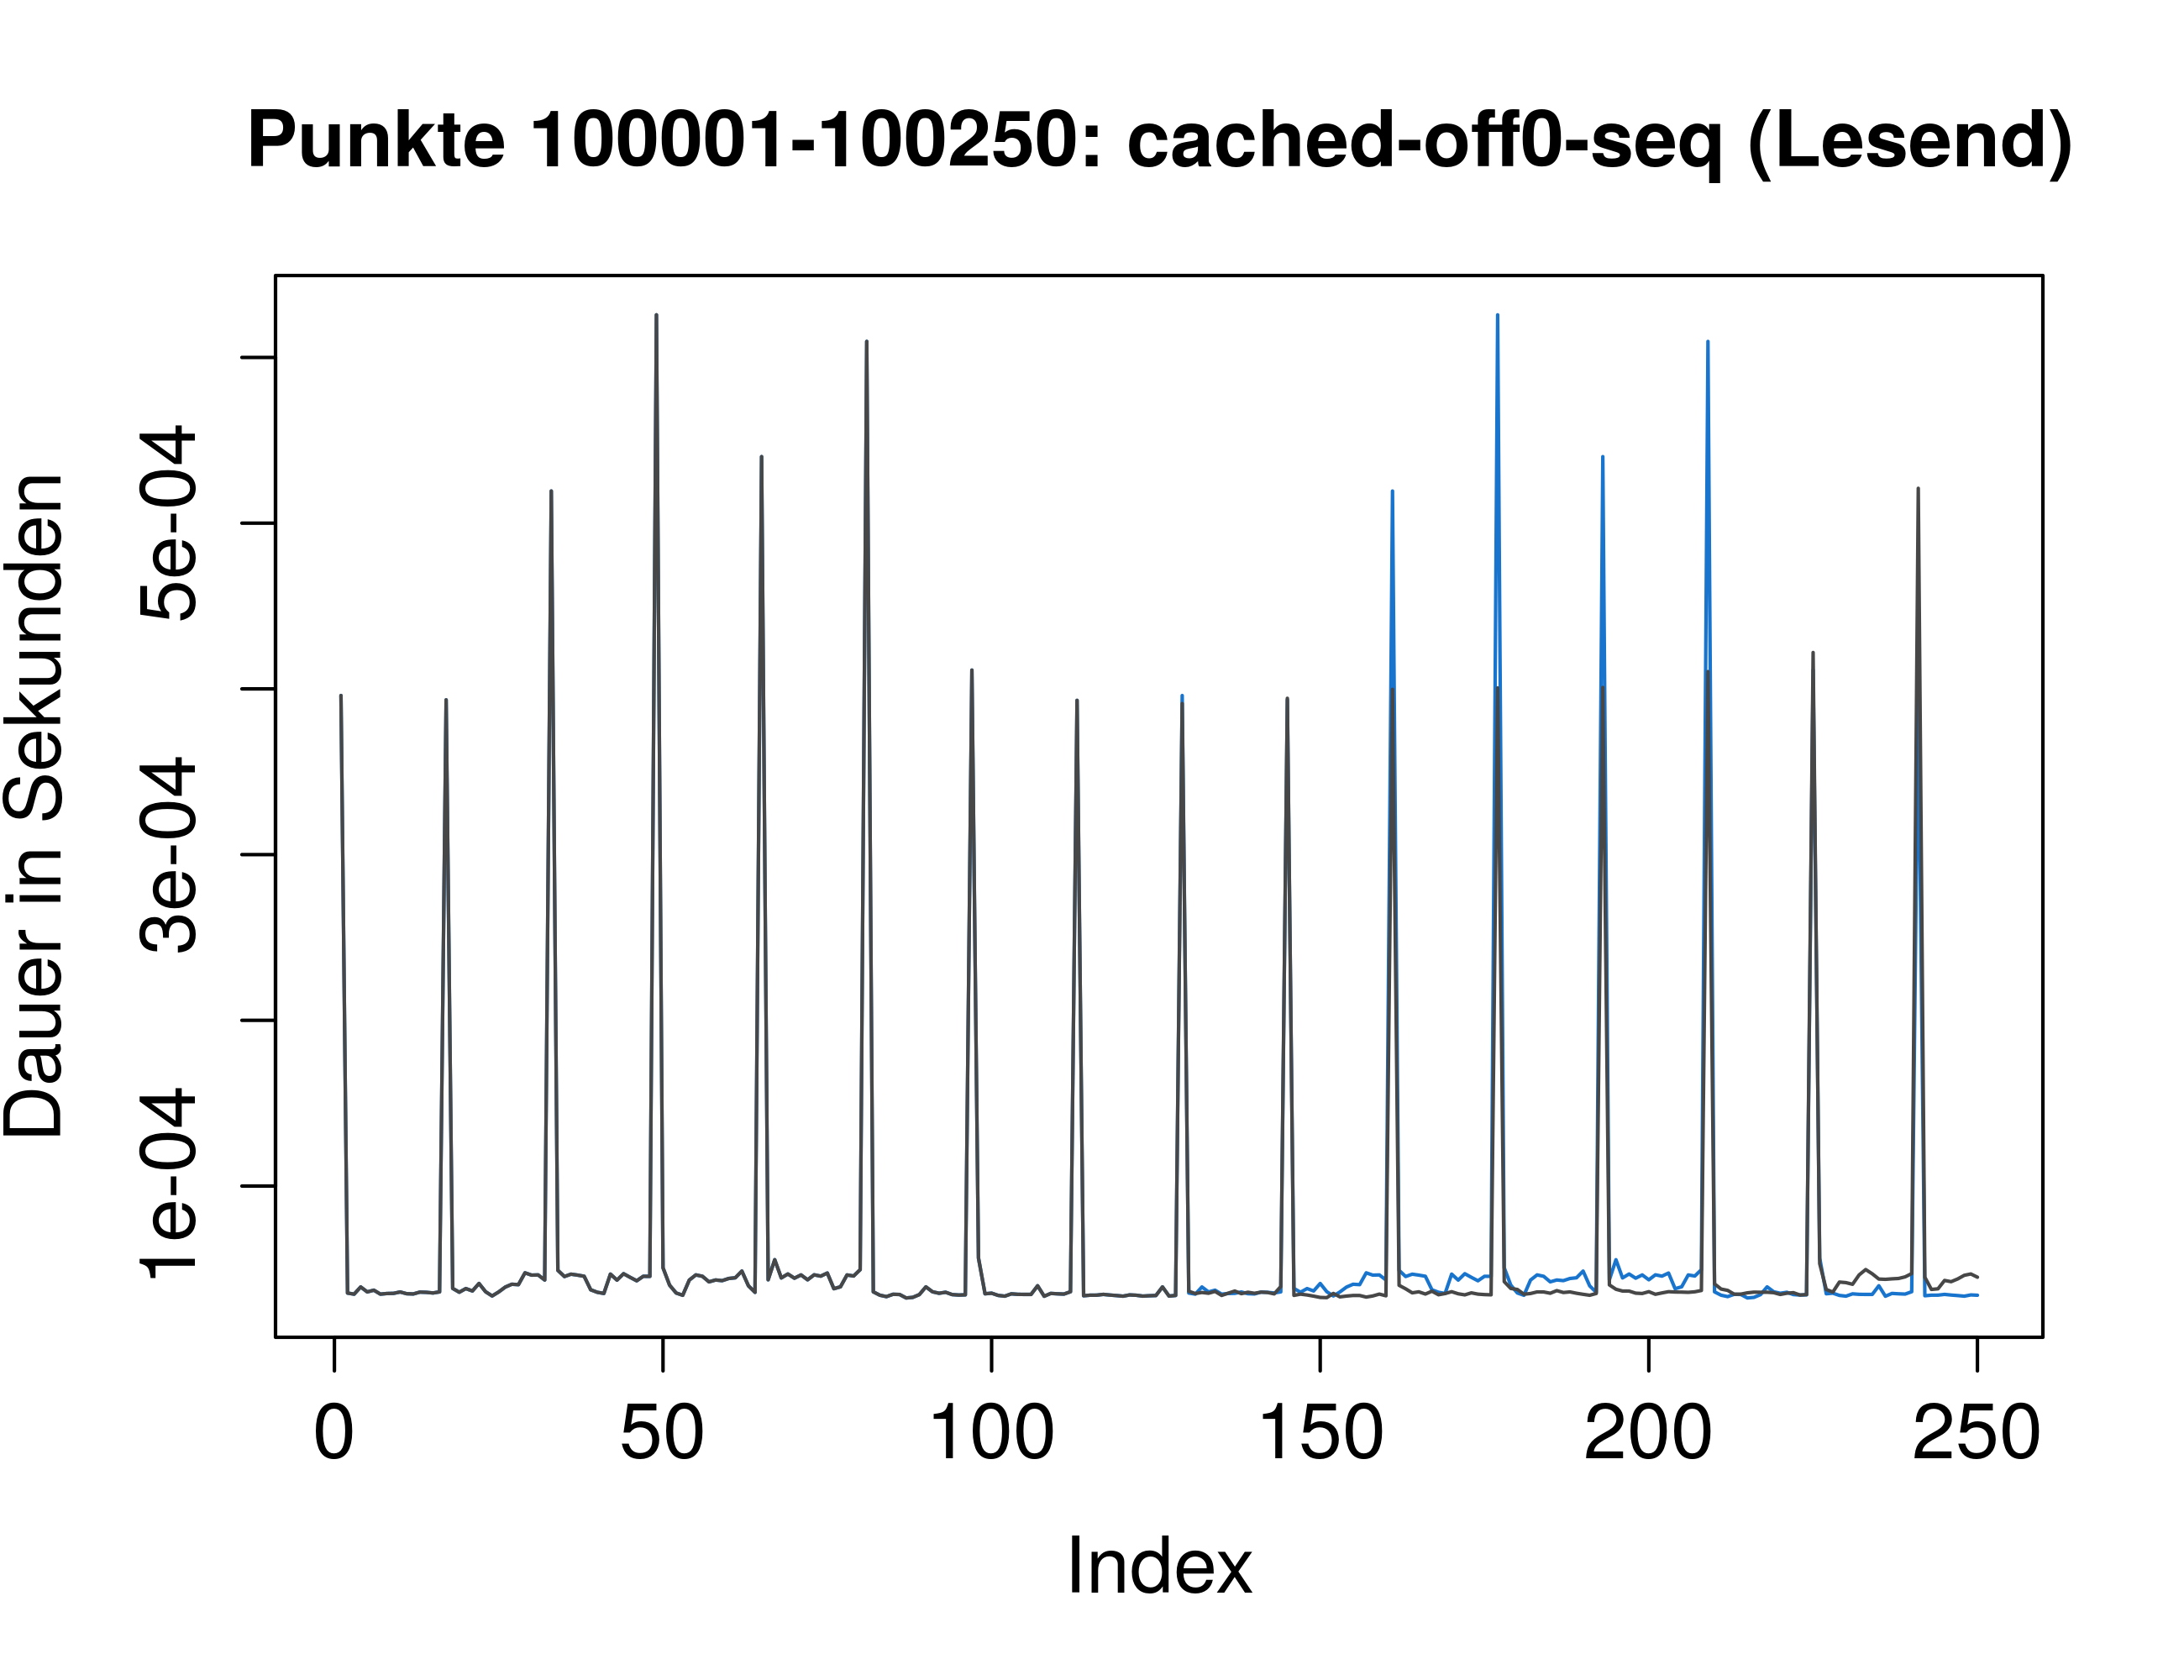
\includegraphics[width=.6\textwidth]{Bilder/Plots/exploration/plot_periodicity100001read_seq.png}
		}	
		\caption{Ausnutzen des periodischen Verhaltens der Zugriffszeiten als erstes einfaches Modell}
		\label{fig:periodicity100001}
	\end{center}
\end{figure} 
\clearpage

\section{Analyse der Fehlerklassen}
\label{eval:fk_analyse}
Alle Modelle werden auf den zusammengeführten Datensätzen aus lesenden und schreibenden Zugriffen angewendet. Daher gibt es im Folgenden nur noch jeweils eine Abbildung zu den sequentiellen und eine zu den Messungen mit zufälligem Dateizugriff.
Zunächst werden zu einer Zugriffsgröße alle Messreihen mit lesenden Aufrufen gezeichnet, danach kommen die schreibenden Zugriffe. 
Die in \ref{fk-modelle} eingeführten Fehlerklassen untersuche ich anhand der Ergebnisse, die aus der Clusteranalyse der Residuen von \textit{LinReg G} entstanden sind.\medskip

Die Laufzeit-Vorhersagen von \textit{LinReg G} werden in \ref{eval:analyse_referenz} genauer betrachtet.
Um den Prozess der Generierung der Fehlerklassen besser zu verstehen, werden die entsprechenden Graphen schon einmal vorgezogen, die Vorhersagen des Modells für beide Datensätze sind in Abbildung \ref{fig:vorgriff_linreg} zu sehen.
Für die Bestimmung der Fehlerklassen werden die Residuen des Modells verwendet, diese ergeben sich aus dem Abstand der vorhergesagten Laufzeiten (in blau) zu den tatsächlichen Laufzeiten (in grau). 

\begin{figure}[!b]
	\centering
	\subfloat[Modell \textit{LinReg G}; Obacht: verschobene Y-Achse]{
		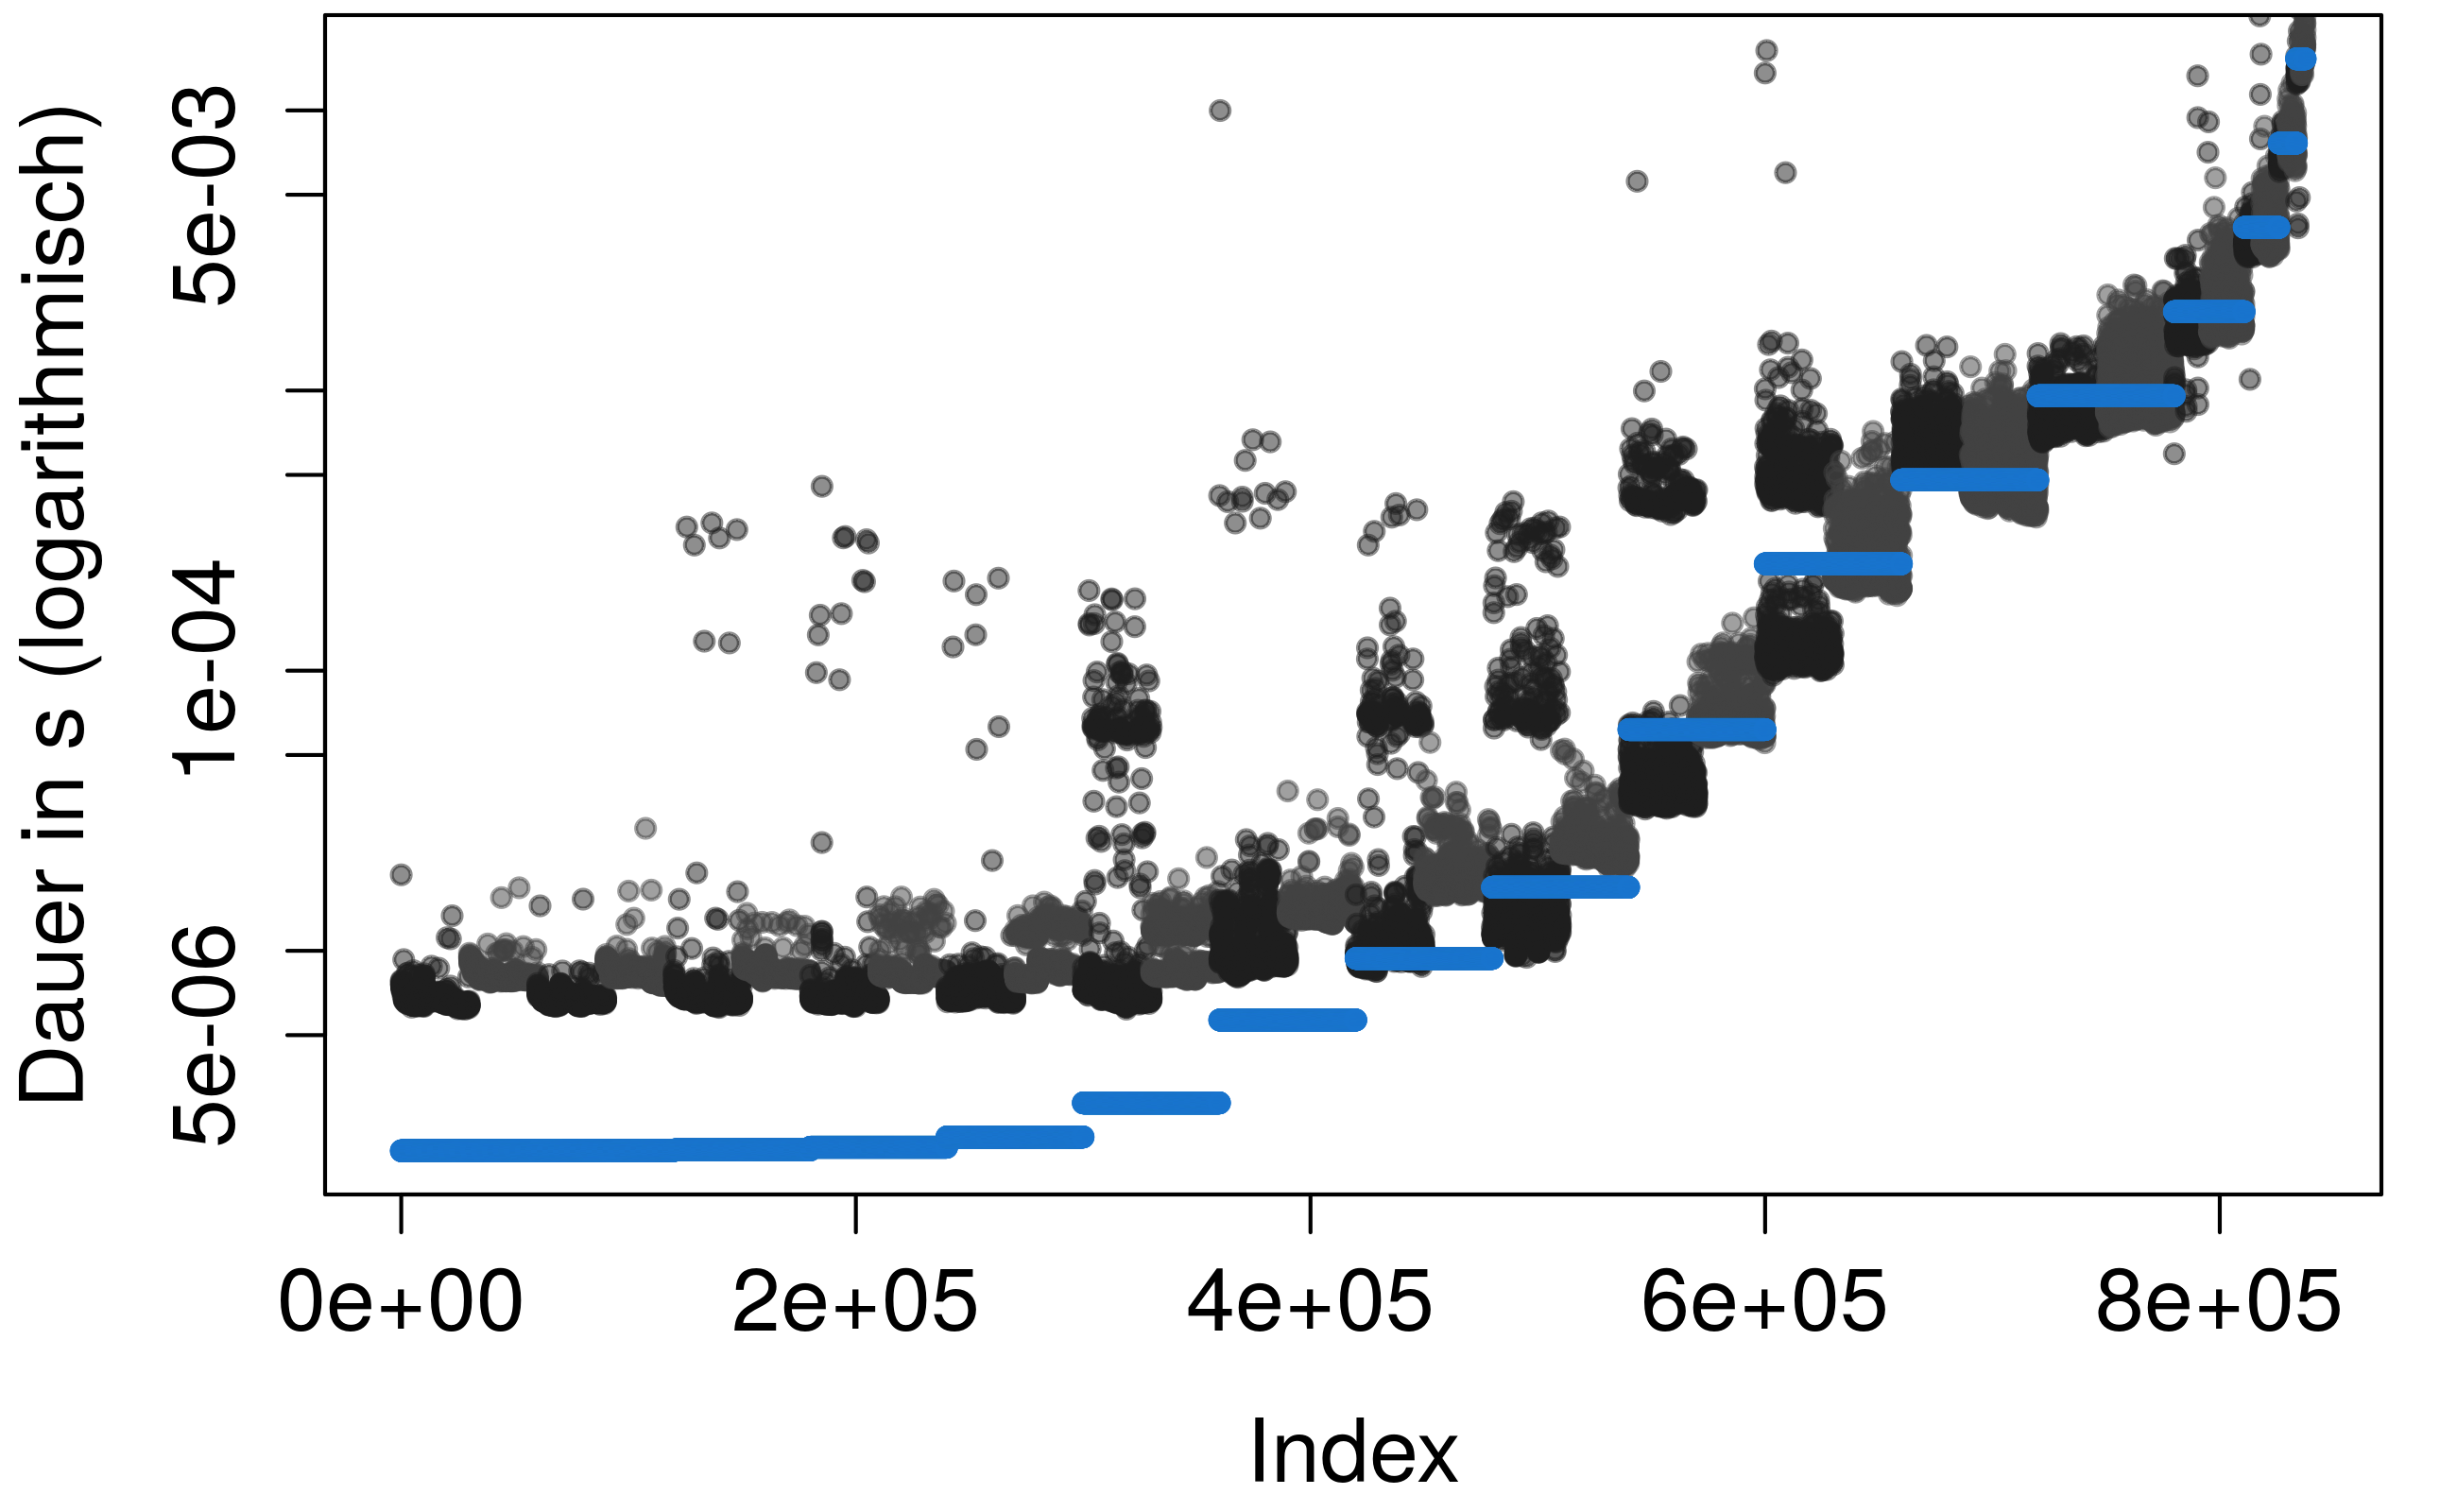
\includegraphics[width=.43\textwidth]{Bilder/Plots/baselines/plot_seq_linreg_Size.png}
	}
	\hfill
	\subfloat[Modell \textit{LinReg G}]{
		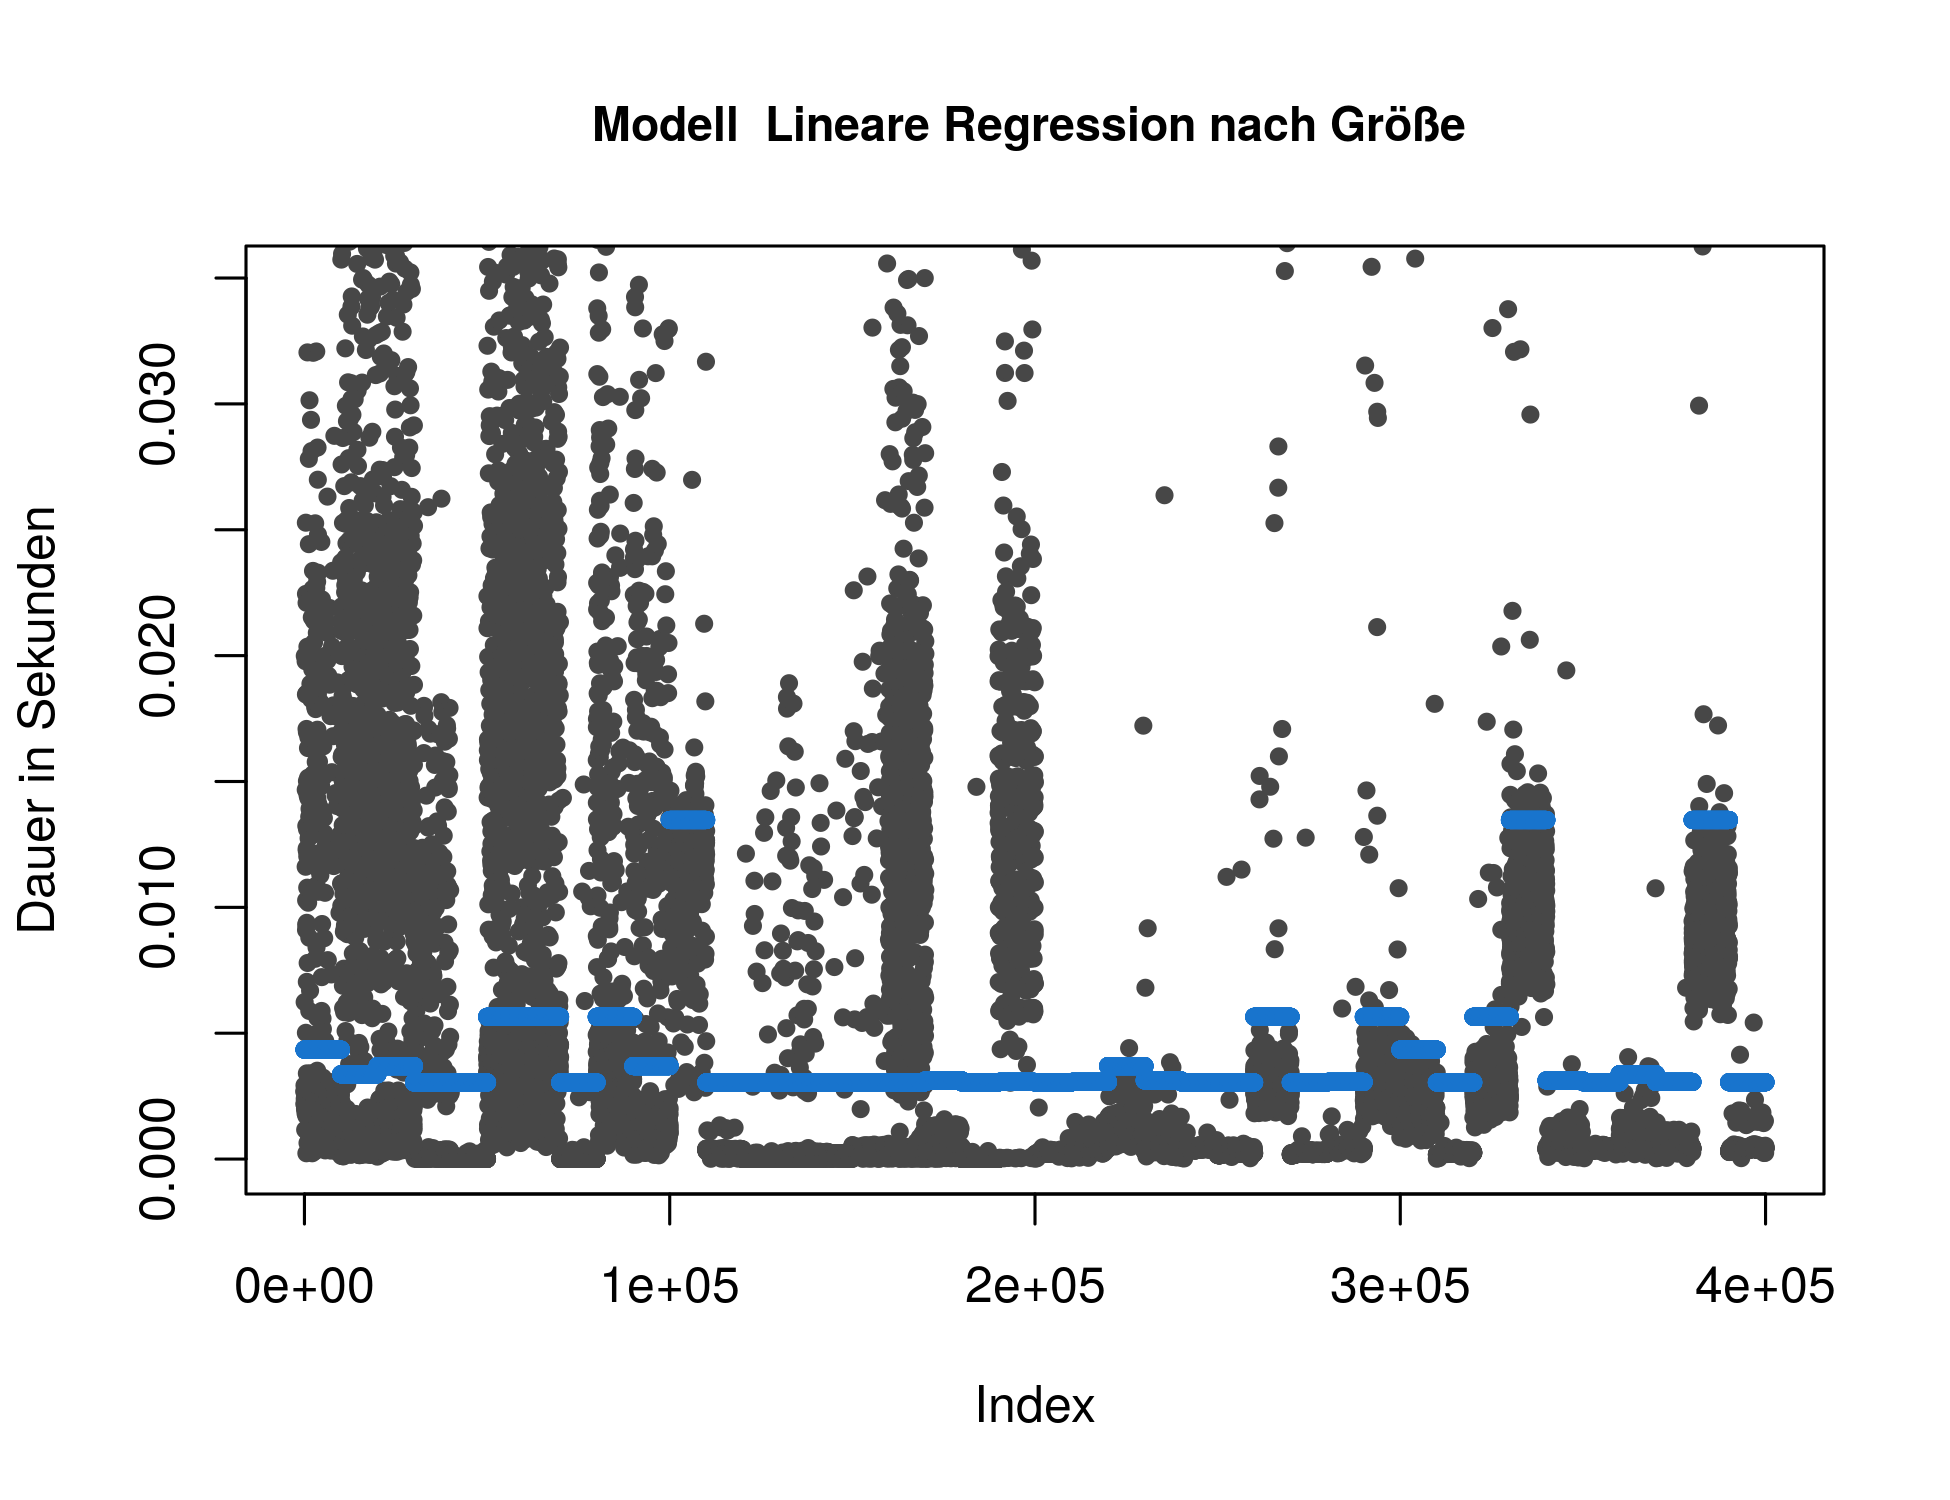
\includegraphics[width=.43\textwidth]{Bilder/Plots/baselines/plot_rnd_linreg_Size.png}
	}
	\caption{Referenzmodell \textit{LinReg G} angewendet auf SEQ (links) und RND (rechts). Die Vorhersagen sind in blau gezeichnet.}
	\label{fig:vorgriff_linreg}
\end{figure} 

In den Abbildungen \ref{fig:error_class_clustering_seq}a und \ref{fig:error_class_clustering_rnd}a sind in Zeitreihe die Residuen aufgezeichnet, die \textit{LinReg G} auf den sequentiell, respektive randomisiert, ausgeführten Messungen mit seinen Vorhersagen gegenüber den tatsächlichen Laufzeiten erreicht hat.
Das Modell \textit{LinReg G} kann nicht zwischen den Operationsarten unterscheiden, auf SEQ führt dies zu etwa gleichen Modellabweichungen für lesende und schreibende Zugriffe, auf RND werden die weit verstreuten Laufzeiten zu lesenden Zugriffen schlechter approximiert.
Die absolute Abweichung wächst bei sequentiellem Zugriff mit der Größe der E/A-Aufrufe, für die zufälligen Zugriffe gilt dies nur bedingt. Auf den kleinsten Zugriffsgrößen werden kleine Fehler gemacht, danach bleibt der Betrag in etwa auf einem Niveau.
Ein Grund für höhere Abweichungen bei Messungen mit längeren Zugriffszeiten ist, dass ein bestimmter relativer Fehler zu entsprechend höheren absoluten Fehlern führt.
Für den plötzlichen und sehr starken Anstieg der Residuen auf höheren Zugriffsgrößen kann dies aber vermutlich nicht die einzige Erklärung sein.

\begin{figure}[t!]
	\centering
	\subfloat[Residuen von \textit{LinReg G} auf SEQ]{
		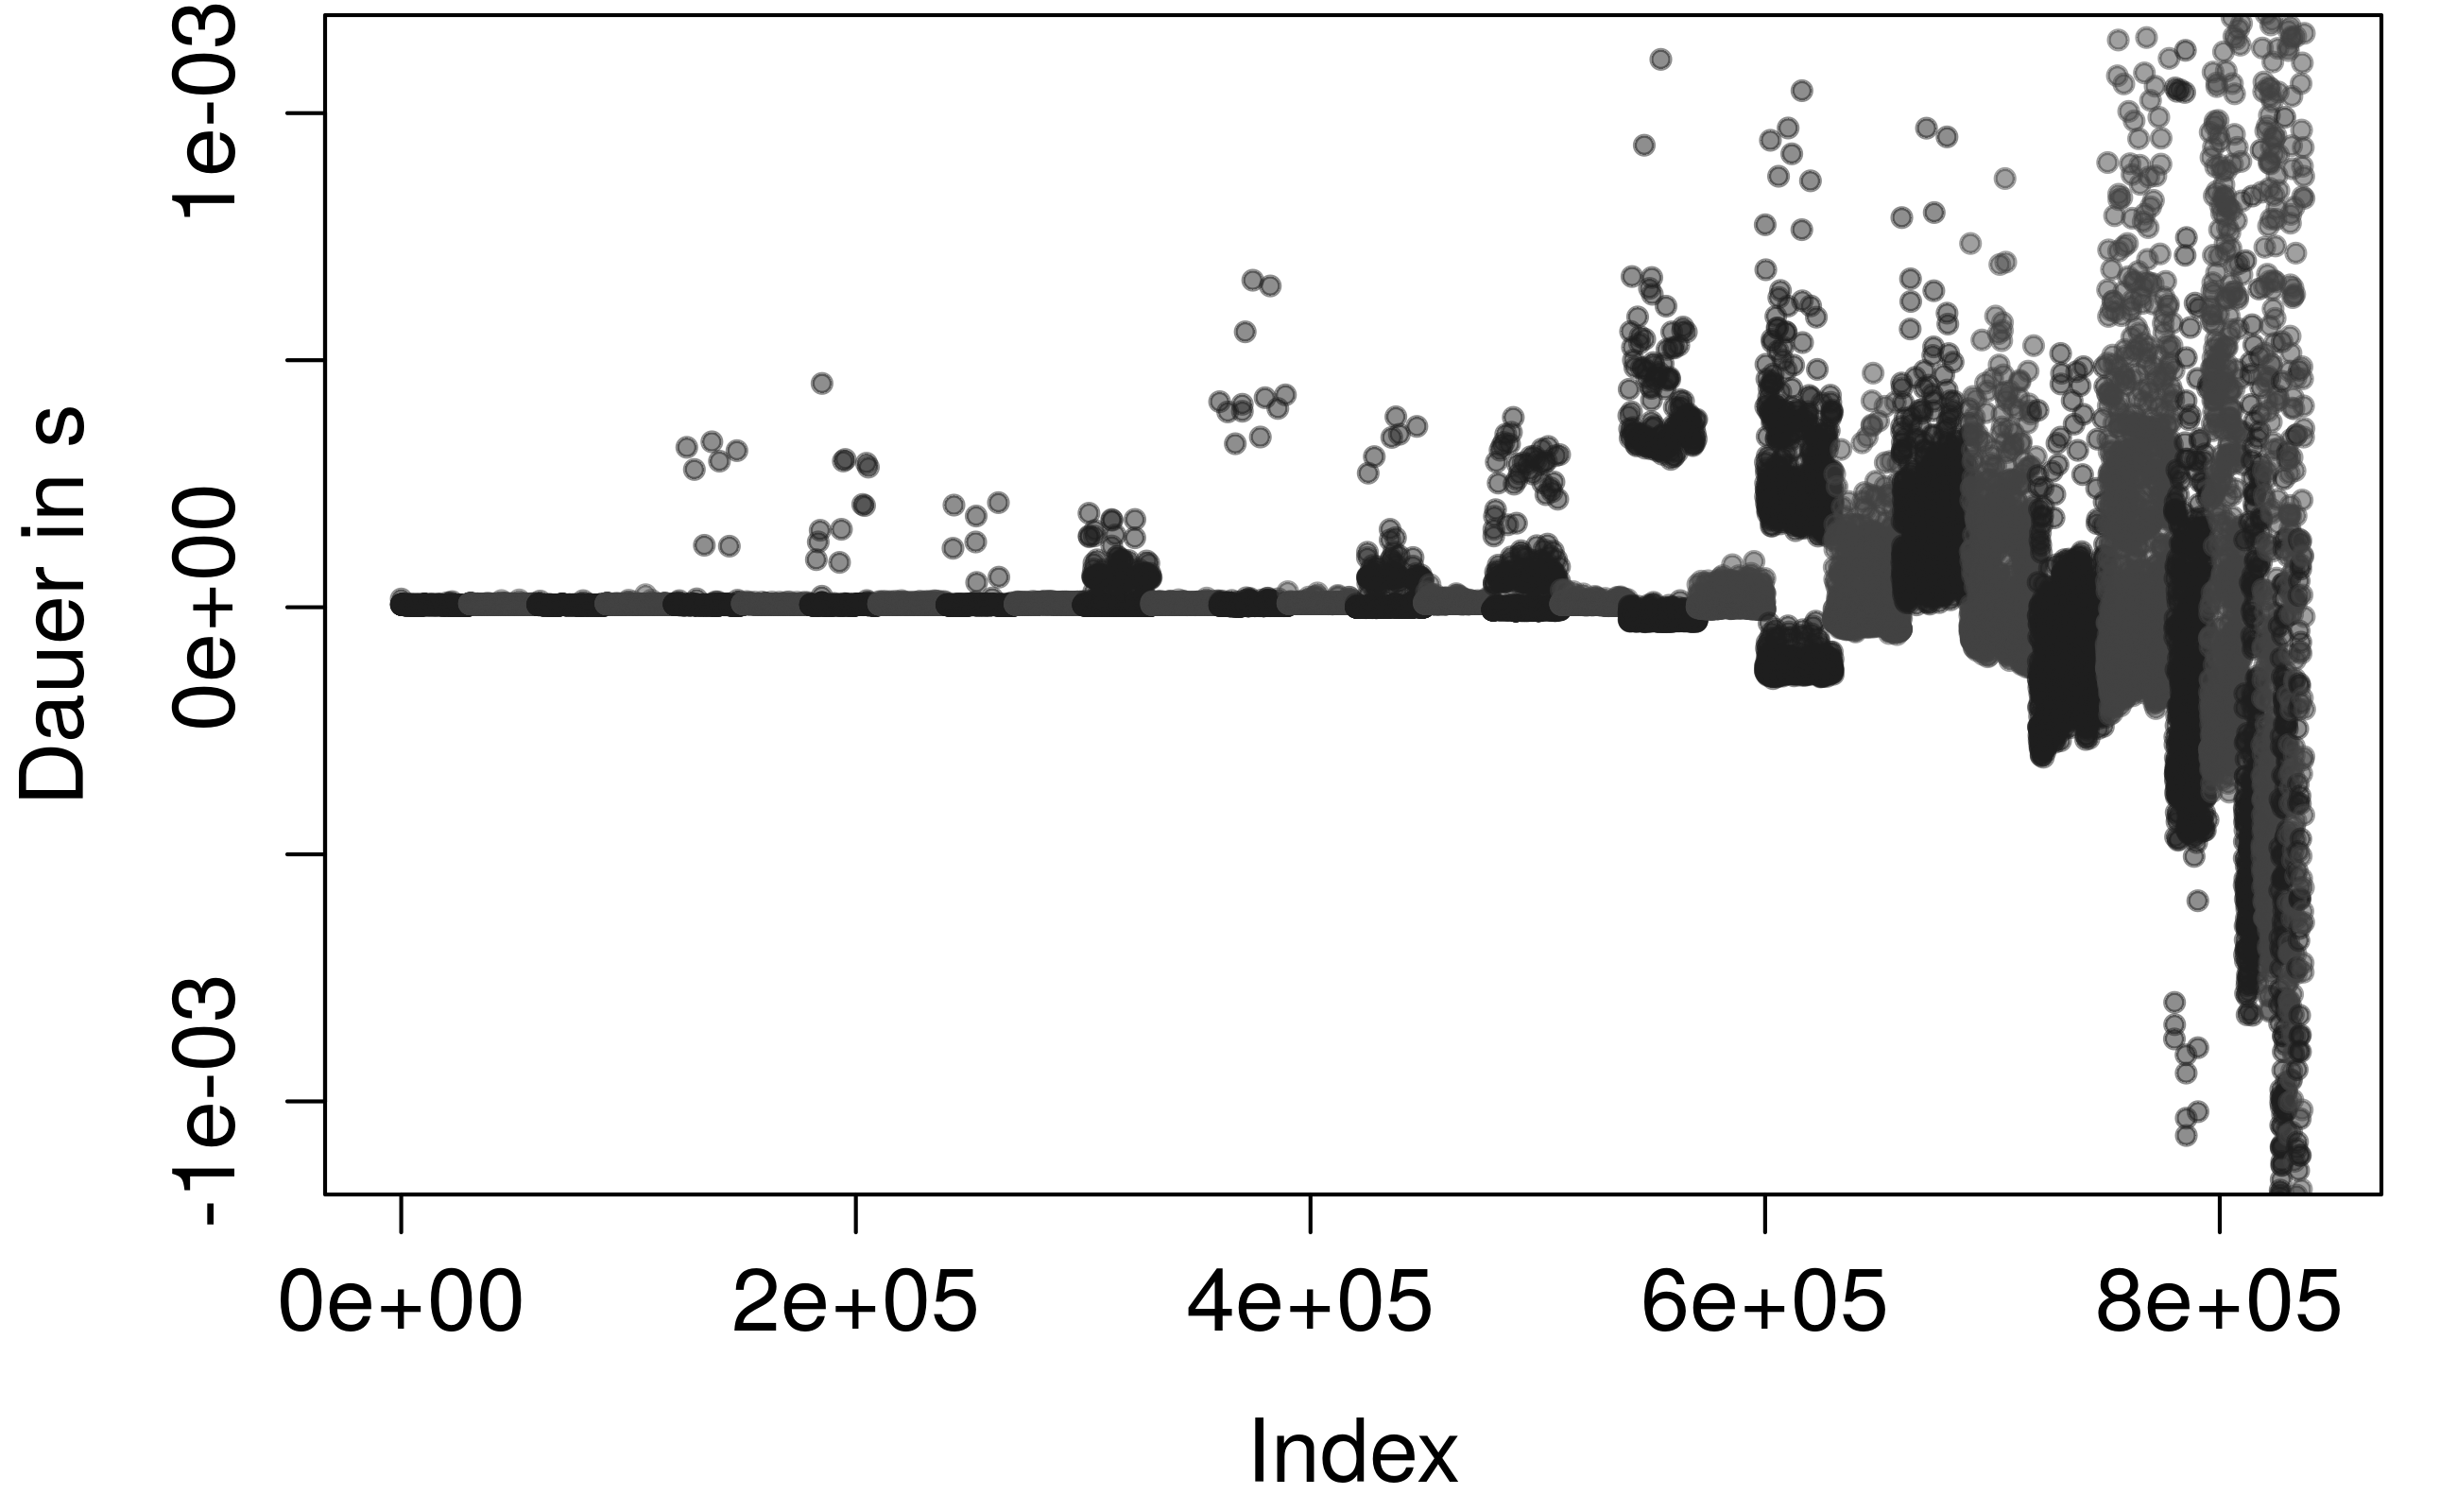
\includegraphics[width=.40\textwidth]{Bilder/Plots/error_class/exploration/linreg_error_seq_all.png}
	}\hfill
	\subfloat[Farblich markierte Fehlerklassen]{
		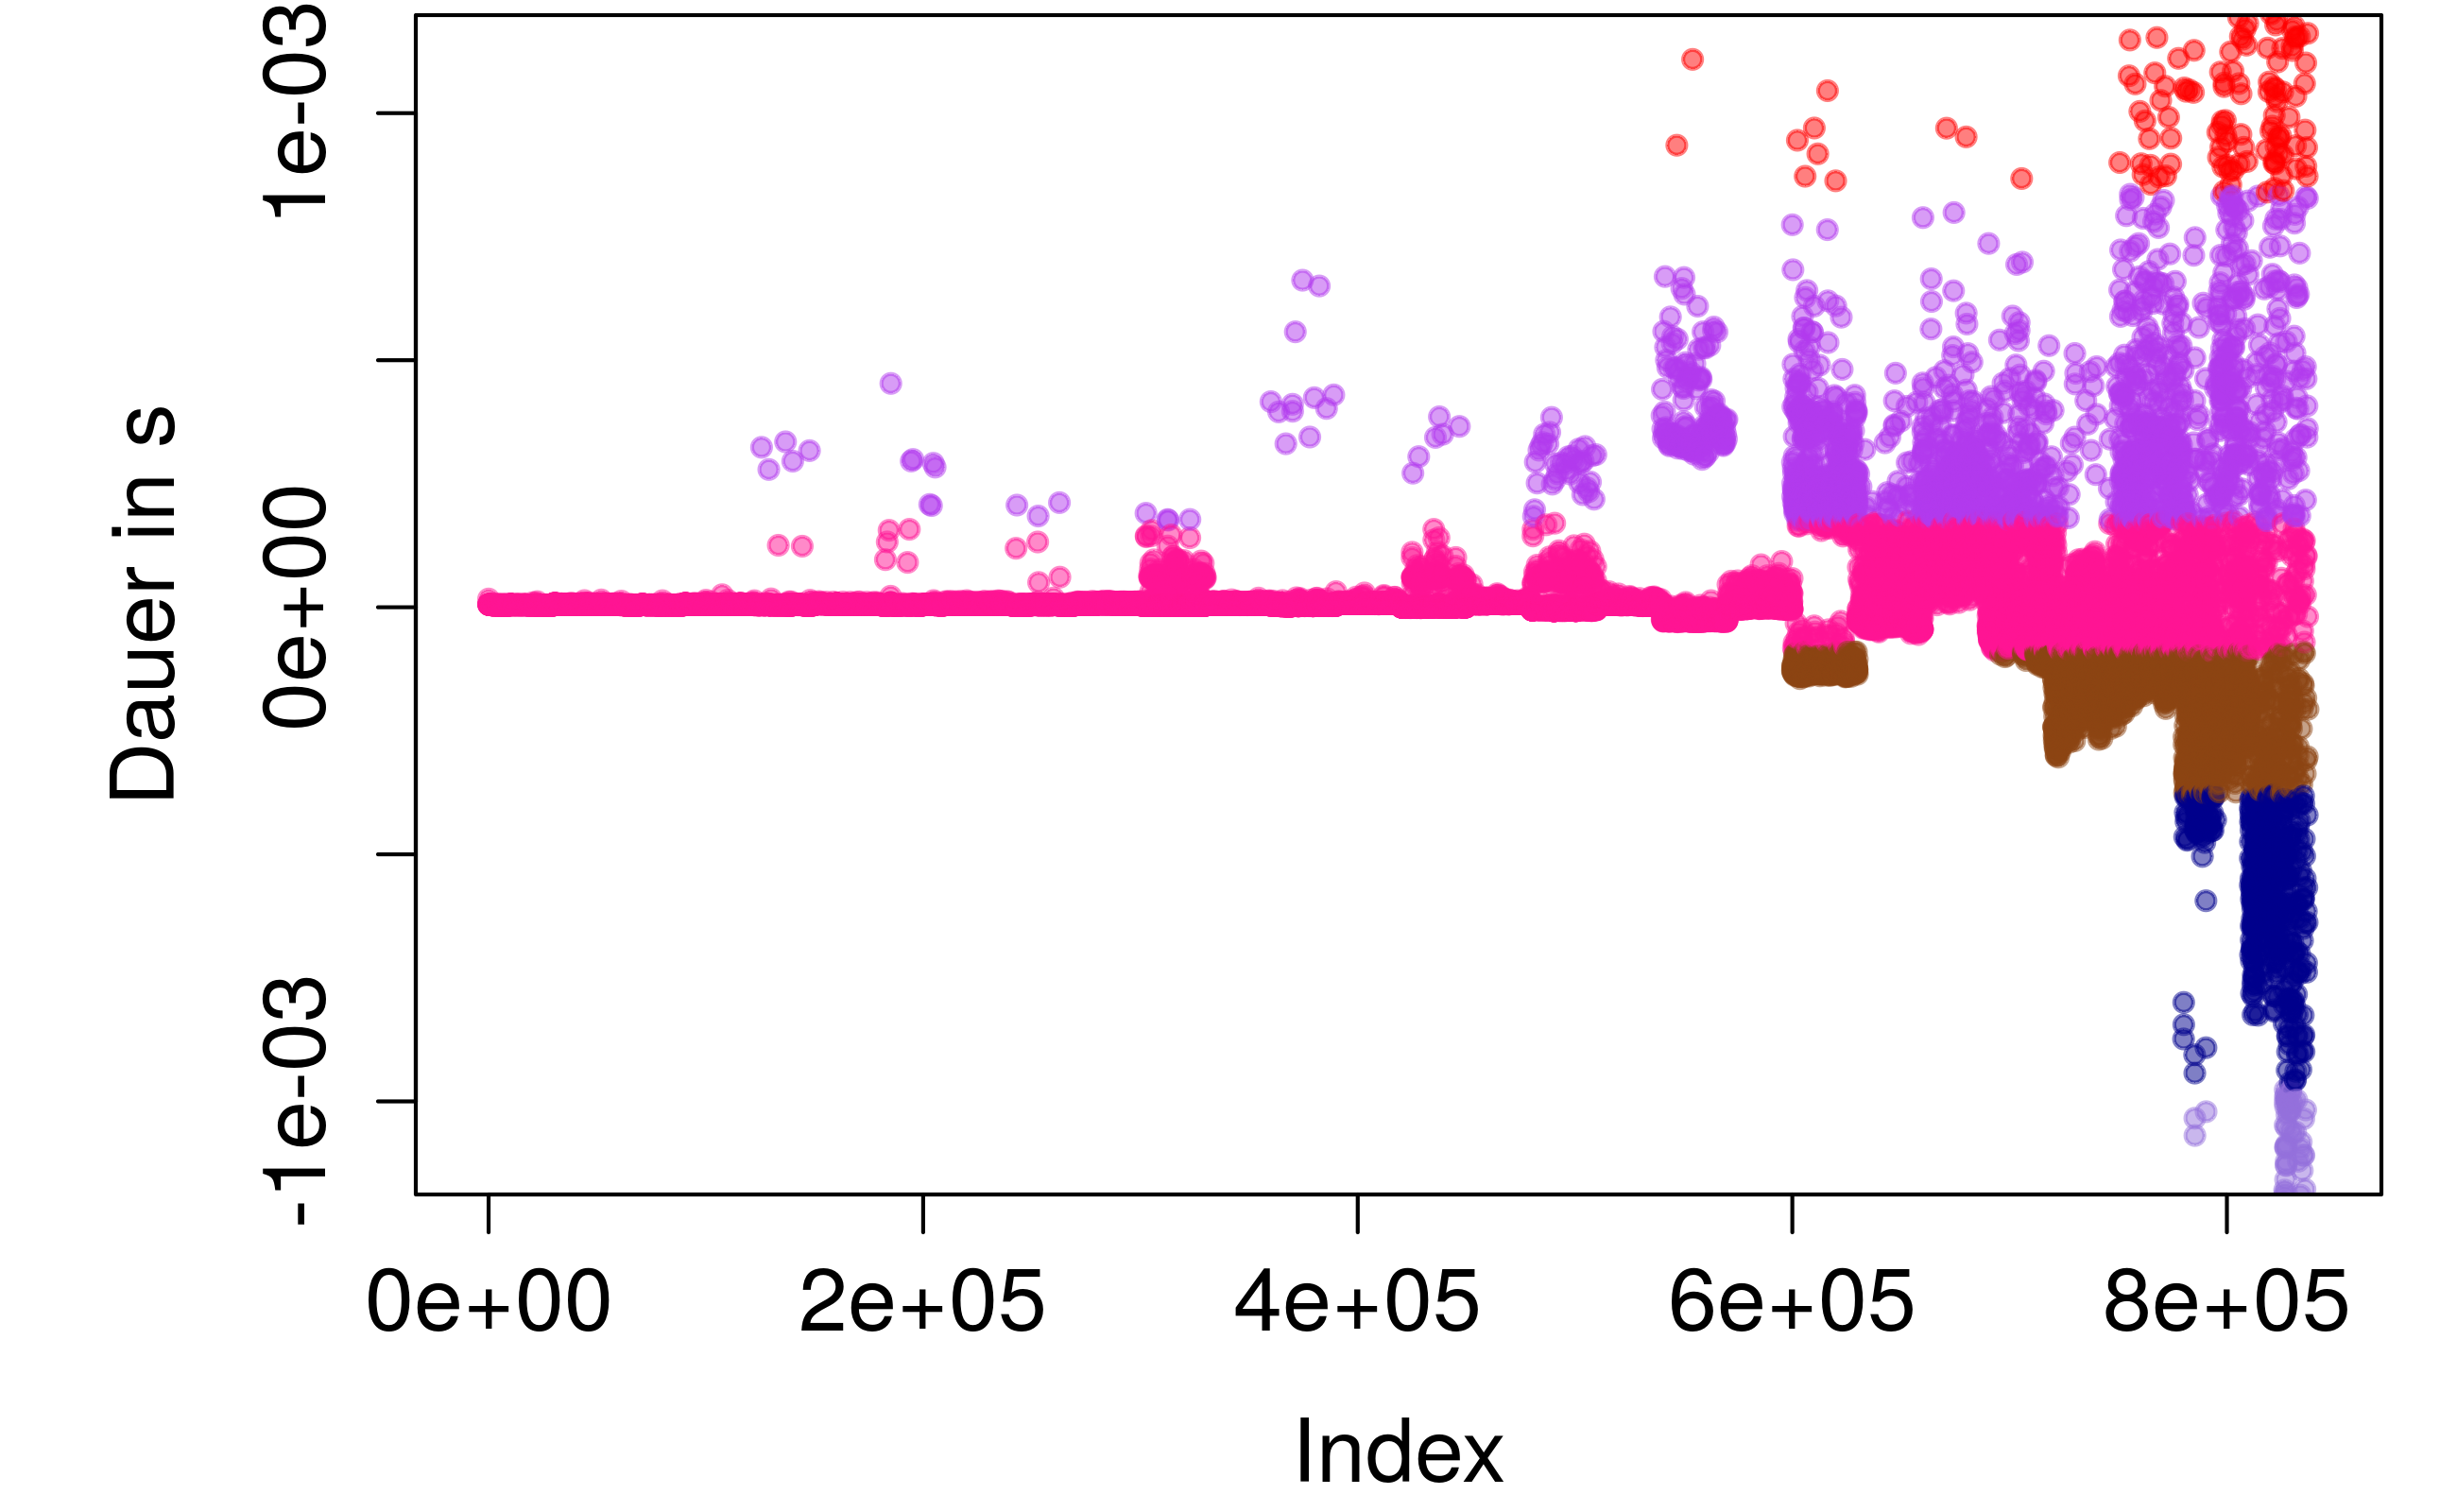
\includegraphics[width=.40\textwidth]{Bilder/Plots/error_class/exploration/linreg_error_clustering_seq_all.png}
	}\\
	\subfloat[sortierte Residuen]{
		\includegraphics[width=.40\textwidth]{Bilder/Plots/error_class/exploration/linreg_error_sorted_clustering_seq.png}
	}\hfill
	\subfloat[Dichte der Klassen um den Nullpunkt]{
		\includegraphics[width=.40\textwidth]{Bilder/Plots/error_class/exploration/density_of_fk_seq.png}
	}
	\vspace*{-0.3cm}
	\caption{Fehlerklassen, die aus den Residuen von \textit{LinReg G} auf SEQ durch eine Cluster-Analyse erstellt wurden}
	\label{fig:error_class_clustering_seq}
\end{figure} 
\begin{figure}[b!]
	\centering
	\subfloat[Residuen von \textit{LinReg G} auf RND]{
		\includegraphics[width=.40\textwidth]{Bilder/Plots/error_class/exploration/linreg_error_rnd_all.png}
	}\hfill
	\subfloat[Farblich markierte Fehlerklassen]{
		\includegraphics[width=.40\textwidth]{Bilder/Plots/error_class/exploration/linreg_error_clustering_rnd_all.png}
	}\\
	\subfloat[sortierte Residuen]{
		\includegraphics[width=.40\textwidth]{Bilder/Plots/error_class/exploration/linreg_error_sorted_clustering_rnd.png}
	}\hfill
	\subfloat[Dichte der Klassen um den Nullpunkt]{
		\includegraphics[width=.40\textwidth]{Bilder/Plots/error_class/exploration/density_of_fk_rnd.png}
	}
	\vspace*{-0.3cm}
	\caption{Fehlerklassen, die aus den Residuen von \textit{LinReg G} auf RND durch eine Cluster-Analyse erstellt wurden}
	\label{fig:error_class_clustering_rnd}
\end{figure} \medskip

In den Graphen \ref{fig:error_class_clustering_seq}b und \ref{fig:error_class_clustering_rnd}b ist durch farbliche Markierung die Zugehörigkeit der Messpunkte zu ihren Fehlerklassen dargestellt.
Die Unterscheidung in verschiedene Klassen findet in horizontalen Linien statt.
Jede Klasse deckt einen bestimmten Bereich der Residuen ab.
Bei den sequentiellen Messungen werden nur die höheren Zugriffsgrößen durch Fehlerklassen differenziert, bei den zufälligen Zugriffen wird bereits bei kleineren Zugriffsgrößen unterschieden. Die auf RND gefunden Fehlerklassen beziehen sich größtenteils auf die lesenden Zugriffe, dies deckt sich mit der Beobachtung in Kapitel \ref{eval:exploration}, dass es in RND-R große Varianzen in den Laufzeiten zu einer Zugriffsgröße gibt.\medskip

Bei der Betrachtung der Graphen, in denen nach Fehler sortiert wurde (Abbildung \ref{fig:error_class_clustering_seq}c und \ref{fig:error_class_clustering_rnd}c ), können die Anzahlen der jeweils zugeordneten Punkte zu den Klassen gut quantifiziert werden.
In beiden Fällen enthält eine Klasse den Großteil der Punkte.
Die Klassen, die Bereiche mit ähnlich großen Residuen abdecken, enthalten noch einen größeren Anteil der Messdaten. Den weiteren Fehlerklassen werden nur sehr wenige Messungen zugeordnet.
Es gibt recht wenig Messungen mit sehr hohen und niedrigen Residuen, die werden allerdings durch mehrere Klassen abgedeckt. So werden die obersten 5\% der Modellabweichungen vom sequentiellen Datensatz in 5 Klassen aufgeteilt.\medskip

Die beiden Abbildungen \ref{fig:error_class_clustering_seq}d und \ref{fig:error_class_clustering_rnd}d zeigen die Dichteverteilungen der Fehlerklasse, die den kleinsten Fehler abdeckt, sowie der nächst kleineren und größeren Fehlerklasse.
Idealerweise sollte die Dichte einer Fehlerklasse nur eine Spitze enthalten. Die Klasse repräsentiert dann genau einen Fehlerbetrag, der dann einem E/A-Pfad entsprechen sollte.
Auf den sequentiellen Daten weisen die Dichten klar voneinander unterscheidbare Spitzen auf.
Ebenso hat die Dichte der Fehlerklasse links vom Nullpunkt sowie die um den Nullpunkt auf RND klar definierte Spitzen. Die Verteilung der Dichte rechts vom Nullpunkt auf den randomisierten Daten weist allerdings keine Spitze auf. Diese Klasse stellt daher keinen E/A-Pfad dar.
Die Fehlerklassen mit mehreren Spitzen hätten unter Umständen noch weiter unterteilt werden müssen, um die E/A-Pfade korrekt darzustellen.
Diese Beobachtungen könnten darauf hinweisen, dass auf den Messungen mit sequentiellem Zugriff eigentlich eine größere Anzahl Cluster-Gruppen benötigt worden wäre, um alle E/A-Pfade zu repräsentieren, während bei den Messungen mit zufälligen Dateizugriffen weniger genutzt werden müssten. \medskip

Das Modell \textit{LinReg G} scheint generell schon recht gut zu sein, da die Fehler sich für die Klassen mit dem kleinsten durchschnittlichen Fehler sammeln.
Es gibt allerdings einige Datenpunkte, die das Modell sehr schlecht vorhersagen konnte. Die Annahme ist nun, dass die Messergebnisse mit stark abweichenden Residuen im Allgemeinen unterschiedlich vom System verarbeitet wurden, sodass Fehlerklassen die unterschiedlichen E/A-Wege im System repräsentieren. 
Dabei muss immer beachtet werden, dass die Vorhersage von Messungen mit höheren Zugriffsgrößen auch zu größeren Abweichungen führt.\\
Ein Modell, das eine Modellierung mit dem zusätzlichen Wissen dieser Klassenzuordnungen vornimmt, sollte die Ausreißer, die \textit{LinReg G} schlecht bestimmt hat, wesentlich besser vorhersagen können.
Für die Vorhersage der vielen Messungen mit Residuen um den Nullpunkt herum hat ein Modell mit Fehlerklasseninformationen jedoch keine weiteren Vorteile. 

\subsubsection{Detailbetrachtung der Fehlerklassen}
\begin{table}
	\centering
	\scriptsize
	\hspace*{-1.6cm}
	\subfloat[Fehlerklassen aus \textit{LinReg G} auf SEQ]{
		\begin{tabular}{|r|r|r|r|r|r|r|r|r|}\hline%
			 & \multicolumn{3}{|c|}{gemittelte Angaben} & \multicolumn{3}{|c|}{Angaben zu den Residuen} & \multicolumn{2}{r|}{zugeordnete Messungen} \\ \hline
			Klasse & Durchsatz (B/s) & Größe (B) & Dauer (s) & Min (s) & Durchschnitt (s) & Max (s) & auf SEQ selbst & auf RND \\ \hline\hline
			\csvreader[late after line=\\\hline]%
			{CSV/error_class/seq_linreg_classes_on_rnd.csv}{tp=\tp,idx = \idx,rndcount=\rndcount,minerror=\minerror, meanerror = \meanerror, maxerror = \maxerror, seqcount = \seqcount, size = \size, duration = \duration}%
			{\idx & \tp & \size & \duration & \minerror & \meanerror & \maxerror & \seqcount & \rndcount}%
		\end{tabular}
	}\\
	\hspace*{-1.6cm}
	\subfloat[Fehlerklassen aus \textit{LinReg G} auf RND]{
		\begin{tabular}{|r|r|r|r|r|r|r|r|r|}\hline%
			& \multicolumn{3}{|c|}{gemittelte Angaben} & \multicolumn{3}{|c|}{Angaben zu den Residuen} & \multicolumn{2}{r|}{zugeordnete Messungen} \\ \hline
			Klasse & Durchsatz (B/s) & Größe (B) & Dauer (s) & Min (s) & Durchschnitt (s) & Max (s) & auf RND selbst & auf SEQ \\\hline\hline
			\csvreader[late after line=\\\hline]%
			{CSV/error_class/rnd_linreg_classes_on_seq.csv}{tp=\tp,idx = \idx,rndcount=\rndcount,minerror=\minerror, meanerror = \meanerror, maxerror = \maxerror, seqcount = \seqcount, size = \size, duration = \duration}%
			{\idx & \tp & \size & \duration & \minerror & \meanerror & \maxerror & \rndcount & \seqcount}%
		\end{tabular}
	}
	\caption{Fehlerklassen sortiert nach durchschnittlichem Residuum}
	\label{tab:error_classes_switched}
\end{table}

In den Tabellen \ref{tab:error_classes_switched} wurden die Fehlerklassen nach dem arithmetischen Mittel der Residuen (Durchschnitt) der enthaltenen Datenpunkte sortiert.
Zu jeder Fehlerklasse wird der von ihnen abgedeckte Bereich der Residuen angegeben, dieser erstreckt sich von der ihm zugeordneten Messung mit dem kleinsten Fehler (Min) bis zu der Messung mit dem größten Fehler (Max).
Desweiteren ist zu jeder Klasse der mittlere Durchsatz in Byte pro Sekunde, die mittlere Zugriffsgröße in Bytes und die mittlere Laufzeit in Sekunden aufgeführt.
Zuletzt wird die Anzahl Datenpunkte, die sich in dem abgedeckten Bereich der Klasse befinden, angegeben, zum einen für den Datensatz auf dem sie erstellt wurden und auch für den jeweils anderen Datensatz.\medskip

An den Anzahlen der Messungen, die den Fehlerklassen zugeordnet wurden (\textit{auf SEQ selbst} bzw. \textit{auf RND selbst}) spiegelt sich wieder, was bereits zuvor beobachtet wurde.
Den Fehlerklassen im Bereich der kleinen Residuen werden sehr viele Messungen zugeordnet. Umso größer der absolute Wert der abgedeckten Residuen ist, desto weniger Messungen gehören zu der Klasse.\medskip

Wenn die Fehlerklassen E/A-Pfade repräsentieren, sollten sie sich durch einen spezifischen Durchsatz kennzeichnen.
Für die Fehlerklassen auf RND wird dies im Wesentlichen auch erreicht.
Den ansteigenden durchschnittlichen Residuen werden abnehmende Durchsätze zugeordnet, es gibt also ein umgekehrt proportionales Verhalten zwischen Residuum und Durchsatz.
Die Fehlerklassen 4, 5 und 6 entsprechen alle etwa dem gleichen Durchsatz, hier scheint es eher eine Differenzierung nach Zugriffsgrößen gegeben zu haben.
Die Zuordnung von Durchsatz zum mittleren Residuum auf SEQ gelingt nicht so erfolgreich.\medskip

Ein Hinweis auf gute Unterscheidung von E/A-Pfaden durch Fehlerklassen ist es, wenn es mehrere Klassen mit gleichen Zugriffsgrößen, aber unterschiedlichen Durchsätzen gibt.
Dafür gibt es auf beiden Datensätzen positive und negative Beispiele.
So haben Klasse 4 und 7 auf SEQ mit $1.8\cdot 10^6$ und $1.6\cdot 10^6$ Bytes sehr ähnliche Zugriffsgrößen, aber mit $1.7\cdot 10^9$ und $6.8\cdot 10^8$ Bytes pro Sekunde einen wesentlich unterschiedlichen Durchsatz.
Klasse 4 und 8 auf RND weisen sogar die gleiche mittlere Zugriffsgröße auf.\\
Insgesamt scheint die Zuordnung von Fehlerklassen zu E/A-Pfaden durchaus zu gelingen, auf RND funktioniert es eventuell noch etwas besser als auf SEQ.

\subsubsection{Anwendung der Fehlerklassen auf dem jeweils anderen Datensatz}
Anhand einer weiteren Betrachtung der Fehlerklassen sollen die Unterschiede zwischen den Klassen auf den beiden Datensätzen analysiert werden.
Dazu werden die Fehlerklassen-Klassifikatoren auf einem Datensatz generiert und auf dem jeweils anderen Datensatz zur Zuordnung der Messungen genutzt.
Eine Skizze zu diesem Ablauf ist in Abbildung \ref{fig:switched_classificators} zu sehen.

\begin{figure}
	\begin{center}
		\subfloat{
			\includegraphics[width=.93\textwidth]{Dot/switched.png}
		}
		\caption{Anwendung der auf SEQ mit \textit{LinReg G} erstellten Fehlerklassen zur Zuordnung der Messungen in RND}
		\label{fig:switched_classificators}
	\end{center}
\end{figure} 

Die Neuzuordnung wurde ebenso gemacht, wie sie vom k-means-Algorithmus durchgeführt wird.
Für alle Klassen wurden die mittleren Residuen nach Zuordnung der Punkte auf dem ursprünglichen Datensatz berechnet und dann wurde jeder Datenpunkt im anderen Datensatz der Klasse zugeordnet, die am nächsten an seinem eigenen Residuum liegt.\medskip

Die Ergebnisse sind einerseits in Abbildung \ref{fig:error_classes_switched} dargestellt und andererseits in den letzten Spalten in den Tabellen \ref{tab:error_classes_switched}a und \ref{tab:error_classes_switched}b beziffert.\\
Für SEQ ist deutlich zu sehen, dass ein Großteil der Punkte derselben Fehlerklasse zugeordnet worden sind. Dadurch findet zwischen den Messungen in der Abbildung \ref{fig:error_classes_switched}a keine Unterscheidung mehr statt.
In der Abbildung \ref{fig:error_classes_switched}b mit sortierten Residuen ist zu erkennen, dass das gesamte Plateau aus Messungen mit Residuen um den Nullpunkt und die Fortsätze in beide Richtungen zu dieser einen Klasse gehören.
Die Zahlen zu \textit{auf SEQ} in Tabelle \ref{tab:error_classes_switched}b bestätigen diese Erkenntnis.
Es befinden sich 836\,841 von von 837\,600 Messungen in derselben Klasse, wenn RND-Fehlerklassen auf SEQ genutzt werden.
Dies ist die Klasse mit kleinstem mittleren Residuum, der auch auf RND selbst ein Großteil der Messungen zugeordnet wurden.\medskip

Dagegen wird bei RND mit Fehlerklassen aus SEQ (Abbildungen \ref{fig:error_class_clustering_rnd}c und \ref{fig:error_class_clustering_rnd}d) in dem Bereich mit kleinerem Fehler nun stärker als zuvor differenziert, während alle Messungen mit größerem Residuum dieselbe Klasse haben.
Die Fehlerklassen von SEQ sind so gesehen recht gut zur Differenzierung der Datenpunkte auf RND nutzbar.
Dies ist auch in Tabelle \ref{tab:error_classes_switched}a den Werten für \textit{RND} zu entnehmen. Die meisten Messungen wurden Klasse 2 zugeordnet, allerdings wurden auch den anderen Klassen einige Messungen zugewiesen.
Dies ist dem Umstand geschuldet, dass die SEQ-Fehlerklassen in dem Bereich mit kleinem Residuum stärker differenzieren als die RND-Fehlerklassen.
Da die allermeisten Messungen aus RND zur Klasse mit dem geringsten Residuum gehören, konnten diese Messungen nun etwas besser unterschieden werden.\medskip

Diese Beobachtungen ergeben sich, da die Aufrufe mit sequentiellen Dateizugriff im Allgemeinen erheblich kleinere Residuen haben, als die Aufrufe mit zufälligem Dateizugriff.

\begin{figure}
	\centering
	\subfloat[Klassen aus RND angewendet auf SEQ]{
		\includegraphics[width=.43\textwidth]{Bilder/Plots/error_class/exploration/rnd_linreg_classes_on_seq.png}
	}\hfill
	\subfloat[Sortiert nach Modellabweichung]{
		\includegraphics[width=.43\textwidth]{Bilder/Plots/error_class/exploration/rnd_linreg_classes_on_seq_sorted.png}
	}\\
	\subfloat[Klassen aus SEQ angewendet auf RND]{
		\includegraphics[width=.43\textwidth]{Bilder/Plots/error_class/exploration/seq_linreg_classes_on_rnd.png}
	}\hfill
	\subfloat[Sortiert nach Modellabweichung]{
		\includegraphics[width=.43\textwidth]{Bilder/Plots/error_class/exploration/seq_linreg_classes_on_rnd_sorted.png}
	}
	\caption{Darstellung der Fehlerklassen, die aus aus dem jeweils anderen Datensatz stammen}
	\label{fig:error_classes_switched}
\end{figure} 
\clearpage

\section{Leistungsvorhersage}
\label{eval:leistungsvorhersage}
Nachdem die aus den Benchmark-Tests erhaltenen Messdaten untersucht und aufbereitet worden sind, werden nun die verschiedenen Modelle auf diese Daten angewendet.
Die Modellabweichungen gegenüber den tatsächlich gemessen Werten können dazu genutzt werden, weitere Informationen über die Beschaffenheit der Messdaten zu erlangen und letztendlich das E/A-System besser zu verstehen.\medskip

Die Modelle werden jeweils auf der Verkettung der Datensätze für lesende und schreibende Zugriffe pro Anwendungsfall gelernt, also auf SEQ und RND.
Die Trainingsdaten der neuronalen Netze bestehen aus 1000 zufällig bestimmte Messungen pro Zugriffsgröße und Operationstyp. Insgesamt stehen dem Netz somit 34000 Datenpunkte zum Lernen zur Verfügung.
Dies sollte eine relevante Stichprobe der Messdaten sein, gleichzeitig bleibt der Trainingsaufwand für die Netze so in einem angemessen Rahmen von einigen Minuten bis wenigen Stunden.
Die restlichen Daten werden als Testdatensatz zur Berechnung der Fehlermetriken verwendet.

\subsection{Analyse der Referenzmodelle}
\label{eval:analyse_referenz}
Die Ergebnisse der in Kapitel \ref{analyse:modelle} beschriebenen Referenzmodelle zu den Fehlermetriken sind in Tabelle \ref{tab:triv} zu sehen.
Zusätzlich zu den Fehlermetriken \textit{MAE}, \textit{MAPE}, \textit{MSPE}, \textit{RQ3} und \textit{MAX}, gibt die Spalte \textit{Typ} an, ob das Modell auf aggregierten Daten (agg) oder auf individuellen Messungen (Ind) in Zeitreihe gelernt wurden.\medskip

\begin{table}
	\centering
	\scriptsize
	\subfloat[Anwendung der Referenzmodelle auf SEQ]{
		\begin{tabular}{|r|r|r|r|r|r|r|}\hline%
			Modell & Typ & MAE (s)  & MAPE (\%) & MSPE (\%) & RQ3 (\%) & RMax (\%) \\\hline\hline
			\csvreader[late after line=\\\hline]%
			{CSV/baselines/latex_baseline_seq_results.csv}{Modell=\Model,MAF=\MAF,RMAF=\RMAF, RMQA = \RMQA, Q3 = \Q3, Max = \Max, Typ = \Typ}%
			{\Model & \Typ & \MAF & \RMAF & \RMQA & \Q3 & \Max}%
		\end{tabular}
	} \\
	\subfloat[Anwendung der Referenzmodelle auf RND]{
		\begin{tabular}{|r|r|r|r|r|r|r|}\hline%
			Modell & Typ & MAE (s)  & MAPE (\%) & MSPE (\%) & RQ3 (\%) & RMax (\%) \\\hline\hline
			\csvreader[late after line=\\\hline]%
			{CSV/baselines/latex_baseline_rnd_results.csv}{Modell=\Model,MAF=\MAF,RMAF=\RMAF, RMQA = \RMQA, Q3 = \Q3, Max = \Max, Typ = \Typ}%
			{\Model & \Typ & \MAF & \RMAF & \RMQA & \Q3 & \Max}%
		\end{tabular}
	}
	\caption{Ergebnisse der Referenzmodelle zu den Fehlermetriken}
	\label{tab:triv}
\end{table}

Eine positive Beobachtung in den Ergebnissen auf SEQ ist zunächst, dass alle Metriken einen ähnlichen Trend der  Modelle aufzeichnen, die Modelle verhalten sich insofern konsistent.
Das gilt im Wesentlichen auch für RND, jedoch hat das Modell \textit{Median agg} einen sehr hohen maximalen Fehler. Dies führt entsprechend zu einem vergleichsweise hohen \textit{MSPE}-Wert, obwohl der relative arithmetische Fehler noch recht gering ist.
Wie bereits vermutet, sind die Vorhersagen auf dem Datensatz mit randomisierten Zugriffen schwieriger zu machen, sodass die Modellabweichungen wesentlich höher sind.
Dies gilt insbesondere für die Modelle, die auf linearer Regression basieren.
Eine Ausnahme bilden die Fehlerklassen-Modelle, diese Modelle können weiterhin sehr gute mittlere Vorhersagen treffen, einige Messungen können auf RND allerdings scheinbar sehr schlecht vorhergesagt werden, sodass \textit{RMax} und \textit{MSPE} höher als beim sequentiellen Datensatz sind.\medskip

Insgesamt sind die Ergebnisse der Referenzmodelle auf SEQ bereits überraschend gut.
Die Modelle \textit{Median Agg} und \textit{LinReg G} haben eine durchschnittliche Modellabweichung von 0.06-0.08 Millisekunden gegenüber den sequentiell durchgeführten Zugriffen.\\
Auf RND erreichen nur die \textit{Median agg}-Modelle gute Werte für die Fehlermetriken.
Da die Aggregate der Attribut-Tupel auf RND allerdings nur wenige Messungen enthalten, ist es in diesem Fall fast so, als würden die \textit{Median-Agg}-Modelle zur Vorhersage die Laufzeiten zu den Messungen schlicht auslesen. Die guten Ergebnisse dieser Modelle auf RND waren also zu erwarten.\\
Die \textit{LinReg}-Modelle erreichen auf RND teilweise kaum bessere Ergebnisse als das \textit{Durschnitts}-Modell.
Durchschnittliche Fehler von mehreren tausend Prozentpunkten können kaum sinnvollen Vorhersagen entsprechen. \medskip

Das Modell, das immer die Durchschnittsdauer vorhersagt, definiert mit seinen Ergebnissen eine absolute untere Grenze, die alle anderen Modelle übertreffen sollten, denn bei diesem Modell geht praktisch keine Expertise in die Vorhersage ein.\\ 
Tatsächlich ist dies auch gegeben. \textit{Durchschnitt} erreicht die höchsten Werte für die Fehlermetriken in beiden Testfällen.
Die Modelle mit aufwendigerer Modellierung halten diesem Anspruch also stand und sind soweit gerechtfertigt. Auch wenn, wie erwähnt, die \textit{LinReg}-Modelle scheinbar kaum lineare Zusammenhänge auf RND ausnutzen können.\medskip

Die Modelle, die Fehlerklassen ausnutzen, erzielen bei beiden Anwendungsfällen sehr gute Ergebnisse.
Ein durchschnittlicher relativer Fehler von $6-7\%$ gegenüber den sequentiellen Messungen bzw. $8-12\%$ gegenüber den randomisierten Messungen durch die Modelle, deutet daraufhin, dass die Vorgänge im E/A-System mit Hilfe der Fehlerklassen im Wesentlichen korrekt repräsentiert werden.
Ob über eine größere Messreihe ein wesentlich geringerer durchschnittlicher Fehler als einige Prozentpunkte überhaupt erreicht werden kann, ist fraglich, da das Messrauschen durch unvorhersehbare Ereignisse sowohl auf System- als auch Bauteilebene in diesen Bereichen eine zu große Bedeutung zukommt. \medskip
 
Die Erkenntnisse, die aus den \textit{LinReg}-Modellen gezogen werden können, sind:
\begin{itemize}
	\item Wie bereits aufgrund der berechneten linearen Korrelationen vermutet werden konnte, kann nur die Zugriffsgröße von der linearen Regression erfolgreich zur Bestimmung der Laufzeit ausgenutzt werden.
	\item Die Hinzunahme des Delta-Offsets führt zu keinen Änderungen an den Ergebnissen, das Delta-Offset kann somit höchstens durch komplexere Modelle zur besseren Vorhersage der Laufzeit genutzt werden.
	\item Die weitere Hinzunahme des Operationstyps verschlechtert die Ergebnisse sogar, scheinbar führt der OpTyp zu widersprüchlichen Informationen über die Laufzeit.	
	\item SEQ lässt sich also bereits sehr gut durch den linearen Zusammenhang zwischen Zugriffsgröße und Laufzeit beschreiben, während für RND diese Abhängigkeit unzureichend für eine gute Bestimmung der Zugriffszeiten ist.
\end{itemize}
 
Aufgrund des geringen Nutzens der Attribute Delta-Offset und OpTyp für die lineare Regression wird im Folgenden nur das Modell über die Zugriffsgröße betrachtet.
Da \textit{LinReg G} auf SEQ wesentlich bessere Werte mit Eingabedaten als individuelle Messungen hat, und die Leistung für \textit{Agg} und \textit{Ind} auf RND in etwa gleichauf sind, wird nur \textit{LinReg G} mit Einzelmessungen berücksichtigt.\\

\subsubsection{Betrachtung der Vorhersagen von Referenzmodellen}
Um genauer zu verstehen, wie die Referenzmodelle die Messdaten annähern, ist es notwendig, sich die vorhergesagten Werte gegenüber den tatsächlichen Werten anzuschauen.
Wie zuvor sind die Messdaten nach Zugriffsgröße und Operationstyp sortiert.\medskip

In den Abbildungen \ref{fig:zeit_baselines_seq} und \ref{fig:zeit_baselines_rnd} sind die vorhergesagten Laufzeiten von \textit{Durchschnitt}, \textit{LinReg G}, \textit{Median Agg} und \textit{LinRegFK Median agg} dargestellt.
Die erreichte Qualität der Vorhersagen der Modelle lässt sich recht gut anhand der Stärke der Differenzierung zwischen den Zugriffsgrößen erkennen:
\begin{itemize}
	\item \textit{Durchschnitt} kann aufgrund der Aggregierung über sämtliche Messungen überhaupt nicht zwischen Messungen differenzieren und erreichte entsprechend die schlechtesten Ergebnisse der Fehlermetriken.
	\item \textit{LinReg G} kann einige Zugriffsgrößen unterscheiden, versagt jedoch bei den kleinsten Zugriffen. Die aufwendigeren Zugriffe können scheinbar recht gut als linear abhängig von der Zugriffsgröße modelliert werden, für die kleineren Größen gilt dies jedoch nicht mehr.
	\item \textit{Median agg} kann durch die Aggregierung nach Attribut-Tupel natürlich alle Größen unterscheiden und erreicht damit unter den Modellen ohne Fehlerklassen die besten Ergebnisse. 
	\item \textit{LinRegFK Median agg} kann, mit Hilfe der Fehlerklassen, zusätzlich innerhalb einer Zugriffsgröße weitere Differenzierungen der Messungen durchführen und erreicht entsprechend die besten Fehlerwerte unter den Referenzmodellen.
	Auf SEQ kann bereits so erkannt werden, dass besonders die höheren Zugriffsgrößen besser von \textit{LinRegFK Median agg} als von \textit{Median agg} modelliert werden können.
	Um die Leistungsunterschiede zwischen \textit{Median agg} und \textit{LinRegFK Median agg} auf RND zu erkennen, ist die Darstellung der Vorhersagen in Zeitreihe eher ungeeignet.
	Beim Vergleich der sortierten Graphen in Abbildung \ref{fig:zeit_baselines_sorted_rnd} ist dagegen klar zu erkennen, dass \textit{Median agg} eine stärkere Streuung bei der Vorhersage der langsameren Messungen aufweist und somit öfter daneben liegt.
	Die zusätzliche Differenzierung des Modells mit Fehlerklassen scheint ausschließlich für die Vorhersage der Messungen mit größeren Zugriffsgrößen eine Rolle zu spielen.
	Das passt zu dem Bild, das wir von der Struktur der Fehlerklassen gewonnen haben, nachdem alle schnellen Messungen in derselben Klasse landen und nur die Langsameren in verschiedene Klassen aufgeteilt werden.
\end{itemize}
\begin{figure}
	\centering
	\subfloat[Modell \textit{Durchschnitt}]{
		\includegraphics[width=.45\textwidth]{Bilder/Plots/baselines/plot_seq_mean_performance.png}
	}
	\hfill
	\subfloat[Modell \textit{LinReg G}; Obacht: verschobene Y-Achse]{
		\includegraphics[width=.45\textwidth]{Bilder/Plots/baselines/plot_seq_linreg_Size.png}
	}\\
	\subfloat[Modell \textit{Median agg}]{
		\includegraphics[width=.45\textwidth]{Bilder/Plots/baselines/plot_seq_median_Duration_aggregated.png}
	}
	\hfill
	\subfloat[Modell \textit{LinRegFK Median agg}]{
		\includegraphics[width=.45\textwidth]{Bilder/Plots/baselines/plot_seq_median_Duration_with_linreg_error_class_aggregated.png}
	}
	\caption{Referenzodelle auf SEQ angewendet. In blau sind die vom Modell vorhergesagten Werte, lesende Zugriffe sind in dunkelgrau und schreibende sind in hellgrau dargestellt}
	\label{fig:zeit_baselines_seq}
\end{figure} 

\begin{figure}
	\centering
	\subfloat[Modell \textit{Durchschnitt}]{
		\includegraphics[width=.45\textwidth]{Bilder/Plots/baselines/plot_rnd_mean_performance.png}
	}
	\hfill
	\subfloat[Modell \textit{LinReg G}]{
		\includegraphics[width=.45\textwidth]{Bilder/Plots/baselines/plot_rnd_linreg_Size.png}
	}\\
	\subfloat[Modell \textit{Median agg}]{
		\includegraphics[width=.45\textwidth]{Bilder/Plots/baselines/plot_rnd_median_Duration_aggregated.png}
	}
	\hfill
	\subfloat[Modell \textit{LinRegFK Median agg}]{
		\includegraphics[width=.45\textwidth]{Bilder/Plots/baselines/plot_rnd_median_Duration_with_linreg_error_class_aggregated.png}
	}
	\caption{Referenzodelle auf RND angewendet. In blau sind die vom Modell vorhergesagten Werte, lesende Zugriffe sind in dunkelgrau und schreibende sind in hellgrau dargestellt}
	\label{fig:zeit_baselines_rnd}
\end{figure} 
\begin{figure}
	\centering
	\subfloat[Modell \textit{Median agg}]{
		\includegraphics[width=.45\textwidth]{Bilder/Plots/baselines/plot_rnd_DurationToPredSorted_median_Duration_aggregated.png}
	}
	\hfill
	\subfloat[Modell \textit{LinRegFK Median agg}]{
		\includegraphics[width=.45\textwidth]{Bilder/Plots/baselines/plot_rnd_DurationToPredSorted_median_Duration_with_linreg_error_class_aggregated.png}
	}
	\caption{Referenzodelle auf RND angewendet. Messungen sortiert nach Laufzeit, es wurde nur jeder 250te Punkt gezeichnet.}
	\label{fig:zeit_baselines_sorted_rnd}
\end{figure} 
\clearpage
\subsubsection{Detailbetrachtung der Vorhersagen von Referenzmodellen}
Die Analyse kleinerer Ausschnitte der Modell-Prognosen kann weitere interessante Zusammenhänge zwischen Messdaten und Modellierung aufdecken.\\
In Abbildung \ref{fig:densities_baselines_seq} ist eine Auswahl an Graphen gezeigt, in denen die Dichten der Laufzeiten für jeweils ein spezifisches Attribut-Tupel dargestellt wurden.
Zusätzlich zur Verteilung der Laufzeiten der Messungen der spezifischen Attribute, wurde der vorhergesagte Wert der verschiedenen Modelle zu diesen Attributen in blau eingezeichnet.
Die schwarze Linie markiert das arithmetische Mittel der Laufzeiten, die grüne ist an der Stelle des 0.1 Quantils der Laufzeiten und die pinke Linie markiert das 0.9 Quantil der Laufzeiten.\\
Zu jedem Graphen werden die Attribute der dargestellten Messungen und der \textit{MAPE} (mean absolute percentage error) des Modells gegenüber diesen Messungen angegeben.\medskip

In Abbildung \ref{fig:densities_baselines_seq}a ist die Vorhersage vom Modell \textit{Durchschnitt} zu einem Attribut-Tupel zu sehen, zu dem das Modell einen seiner geringsten \textit{MAPE}-Werte erreicht hat.
Die Vorhersage ist dennoch nicht sehr genau, da der vom Modell geschätzte Wert wesentlich näher am 0.1 Quantil ist, als am tatsächlichen Mittelwert.
Es ist zusehen, dass es eine typische Laufzeit zu diesen Attributen gibt, dort hat die Dichte seine Spitze. Für die Messungen mit dieser Laufzeit wurde vermutlich derselbe E/A-Pfad verwendet. Es gibt aber auch einige Laufzeiten mit größeren Werten.
Anhand des lokalen Maximums bei $6\cdot 10^-4$ Sekunden kann wohl der am zweithäufigsten genommene E/A-Pfad erkannt werden.\medskip

Das Attribut-Tupel zu dem \textit{LinReg G} die Vorhersagen mit seinem geringsten \textit{MAPE} erreicht hat, ist in Abbildung \ref{fig:densities_baselines_seq}b dargestellt.
Der vorhergesagte Wert befindet sich ziemlich genau am Maximum der Dichtefunktion. Entsprechend sagt dieses Modell für eine möglichst große Anzahl Messungen den richtigen Wert voraus. Dies führt allerdings nicht zum kleinst möglichen \textit{MAPE}-Wert, dieser würde auf der schwarzen Linie erreicht werden.\medskip
 
In Abbildung \ref{fig:densities_baselines_seq}c ist die vorhergesagte Laufzeit von \textit{LinRegFK Median agg} eingezeichnet.
Die Vorhersage des Modells zu diesem Attribut-Tupel liegt ziemlich genau auf dem Wert des arithmetischen Mittels der Laufzeiten, sodass der \textit{MAPE} hier gerade minimal wird.\medskip

Als letztes Beispiel wird der Verlauf der Laufzeit-Dichte eines Attribut-Tupels gezeigt, zu dem das Modell \textit{Median agg} eine seiner größten Modellabweichungen erreicht hat.
Interessanterweise sind die Residuen für dieses Attribut-Tupel sehr groß, dabei ist der vorhergesagte Wert des Modells in direkter Nähe des tatsächlichen arithmetischen Mittelwerts der Laufzeiten.
Scheinbar gibt es zwei E/A-Pfade, die etwa mit gleicher Häufigkeit für Messungen mit diesem Attribut-Tupel genommen wurden. 
Das \textit{Median agg}-Modell, das für alle Messungen eines Attribut-Tupels dieselbe Laufzeit vorhersagt, macht gegenüber solchen E/A-Aufrufen, die nicht hauptsächlich denselben E/A-Pfad nehmen, zwangsweise ungenaue Vorhersagen. \medskip

Nach dieser Betrachtung lässt sich feststellen:
Ein Modell, das für alle Messungen eines Attribut-Tupels denselben Wert vorhersagt, kann zu den gemachten Messungen nicht immer kleine Residuen erreichen.
Eine weitere Unterscheidung von Messungen innerhalb eines Attribut-Tupels kann mit den verfügbaren Messdaten allerdings nur durch eine Betrachtung der zeitlichen Abhängigkeit des E/A-Aufrufs von den vorherigen gelingen.\\
Alternativ kann ein Ansatz wie die Zuhilfenahme von Fehlerklassen zur besseren Modellierung verwendet werden, dies ist aber natürlich \glqq unfair\grqq{}, da in den Klassen Informationen über die tatsächliche Laufzeit der E/A-Aufrufe stecken.
 
 \begin{figure}
 	\centering
 	\subfloat[Modell \textit{Durchschnitt} auf SEQ. \textit{MAPE} = 20.77\%, Zugriffsgröße = Delta-Offset = 512\,KiB, OpTyp = W]{
 		\includegraphics[width=.43\textwidth]{Bilder/Plots/baselines/Dichten/plot_density_best_mean_performance.png}
 	}\hfill
 	\subfloat[Modell \textit{LinReg G} auf SEQ. \textit{MAPE} = 6.74\%, Zugriffsgröße = Delta-Offset: 64\,KiB, OpTyp: W]{
 		\includegraphics[width=.43\textwidth]{Bilder/Plots/baselines/Dichten/plot_density_best_linreg_Size.png}
 	}\\
 	\subfloat[Modell \textit{LinRegFK Median agg} auf SEQ. \textit{MAPE} = 2.6\%, Zugriffsgröße = Delta-Offset = 8\,MiB, OpTyp = W]{
 		\includegraphics[width=.43\textwidth]{Bilder/Plots/baselines/Dichten/plot_density_best_median_Duration_with_linreg_error_class_aggregated.png}
 	}\hfill
 	\subfloat[Modell \textit{Median agg} auf SEQ. \textit{MAPE} = 68.65\%, Zugriffsgröße = Delta-Offset = 512\,KiB, OpTyp = W]{
 		\includegraphics[width=.43\textwidth]{Bilder/Plots/baselines/Dichten/plot_density_worst_median_Duration_aggregated.png}
 	} 
 	
 	\caption{Laufzeit-Dichte einiger Referenzodelle auf SEQ; 90\% der Werte sind größer als die grüne, 10\% sind größer als die pinke Linie, die mittlere Laufzeit entspricht der schwarzen Linie, die blaue Linie markiert die Vorhersage des Modells zu diesen Attributen}
 	\label{fig:densities_baselines_seq}
 \end{figure} 
\clearpage

\subsection{Analyse der NN-Modelle}
Die Analyse zu den komplexeren Modellen, die auf neuronalen Netzen basieren, ist dreigeteilt. 
\begin{itemize}
	\item Es wird zu jedem Modell das neuronale Netz betrachtet, das bei der Untersuchung des Parameterraums gefunden wurde und den geringsten \textit{MSPE}-Wert erzielt hat.
Informationen über die Struktur der gefundenen Netze und den Aufwand des Trainingsprozesses finden sich in Tabelle \ref{tab:model-stats}. Im Detail sind dies die Anzahl der verdeckten Schichten, die Anzahl Neuronen pro Schicht, die Anzahl Iterationen, die der Algorithmus gebraucht hat, bis der Schwellenwert für die Konvergenz erreicht war und die Trainingsdauer, also wie lange die Berechnung des Netzes tatsächlich gedauert hat.
	\item In Tabelle \ref{tab:results} sind für alle NN-Modelle die Werte der verschiedenen Fehlermetriken angegeben, zusätzlich sind zum Vergleich die Referenzmodelle \textit{Durchschnitt}, \textit{LinReg G} angewendet auf individuelle Messungen und \textit{LinRegFK Median agg} aufgelistet.
	\item Die Tabelle \ref{tab:outlier} wird für die Analyse der Ausreißervorhersage betrachtet. In der Tabelle sind alle beschriebenen Fehlermetriken zu den NN-Modellen auf SEQ angegeben. Wie bereits beschrieben wurde, gibt es bei den Messungen mit zufälligen Dateizugriffen zu wenig Messungen pro Attribut-Tupel, um die Ausreißervorhersage auf diesen Daten sinnvoll zu betrachten.
\end{itemize}
Im Folgenden werden zunächst einige Beobachtungen zu verschiedenen Bereichen auf den Testergebnissen geschildert, dann werden im Detail die Ergebnisse von den Modellen \textit{NN-Tupel1} und \textit{NN-LinRegFK} betrachtet.

\begin{table}
	\centering
	\scriptsize
	\subfloat[NN-Modelle auf SEQ]{
		\begin{tabular}{|r|r|r|r|r|}\hline%
			Modell & verdeckte Schichten & Neuronen & Iterationen & Trainingsdauer (s) \\\hline\hline
			\csvreader[late after line=\\\hline]%
			{CSV/models/latex_seq_net-stats.csv}{Modell=\Model,verdeckteSchichten=\verdeckteSchichten,Neuronen=\Neuronen, Iterationen = \Iterationen, Trainingsdauer = \Trainingsdauer}%
			{\Model & \verdeckteSchichten & \Neuronen & \Iterationen & \Trainingsdauer}%
		\end{tabular}
	} \\
	\subfloat[NN-Modelle auf RND]{
		\begin{tabular}{|r|r|r|r|r|}\hline%
			Modell & verdeckte Schichten & Neuronen & Iterationen & Trainingsdauer (s) \\\hline\hline
			\csvreader[late after line=\\\hline]%
			{CSV/models/latex_rnd_net-stats.csv}{Modell=\Model,verdeckteSchichten=\verdeckteSchichten,Neuronen=\Neuronen, Iterationen = \Iterationen, Trainingsdauer = \Trainingsdauer}%
			{\Model & \verdeckteSchichten & \Neuronen & \Iterationen & \Trainingsdauer}%
		\end{tabular}
	}
	\caption{Informationen über die erfolgreichsten Neuronalen Netze}
	\label{tab:model-stats}
\end{table}

\begin{table}
	\centering
	\scriptsize
%	\makebox[\textwidth][c]{
	\hspace*{-0.3cm}
		\subfloat[Fehlermetriken auf SEQ]{
			\begin{tabular}{|p{2cm}|r|p{1.4cm}|p{1.4cm}|r|r|r|r|r|}\hline%
				Modell & MAE (s) & Avg- \mbox{MAPE (\%)} & Train- \mbox{MAPE (\%)} &  MAPE (\%) & MSPE (\%) & RQ3 (\%) & RMax (\%) & In-range (\%) \\\hline\hline
				\csvreader[late after line=\\\hline]%
				{CSV/models/latex_seq_results.csv}{Modell=\Model,MAF=\MAF,RMAF=\RMAF, RMQA = \RMQA, Q3 = \Q3, Max = \Max,RMAFTraining = \RMAFTraining, Bereich = \Bereich, RMAFavg = \RMAFavg}%
				{\Model & \MAF & \RMAFavg & \RMAFTraining & \RMAF & \RMQA & \Q3 & \Max & \Bereich}%
			\end{tabular}
%		}
	}\\
%	\makebox[\textwidth][c]{
	\hspace*{-0.3cm}
		\subfloat[Fehlermetriken auf RND]{
			\begin{tabular}{|p{2cm}|r|p{1.4cm}|p{1.4cm}|r|r|r|r|r|}\hline%
				Modell & MAE (s) & Avg- \mbox{MAPE (\%)} &  Train- \mbox{MAPE (\%)} & MAPE (\%) & MSPE (\%) & RQ3 (\%) & RMax (\%) & In-range (\%) \\\hline\hline
				\csvreader[late after line=\\\hline]%
				{CSV/models/latex_rnd_results.csv}{Modell=\Model,MAF=\MAF,RMAF=\RMAF, RMQA = \RMQA, Q3 = \Q3, Max = \Max,RMAFTraining = \RMAFTraining, Bereich = \Bereich, RMAFavg = \RMAFavg}%
				{\Model & \MAF & \RMAFavg & \RMAFTraining & \RMAF & \RMQA & \Q3 & \Max & \Bereich}%
			\end{tabular}
%		}
	}
%	\vspace*{-0.3cm}
	\caption{Ergebnisse der NN-Modelle und einiger Referenzmodelle}
	\label{tab:results}
\end{table}

\subsubsection{Strukturen der neuronalen Netze}
Die Strukturen der erhaltenen neuronalen Netze sind teilweise recht erstaunlich.
Einige Netze sind äußerst komplex.
So hat beispielsweise das erhaltene Netz zu \textit{NN-Tupel1FK} auf RND 17 verdeckte Schichten mit jeweils 28 Neuronen.
Das Lernverfahren zum Erstellen des Netzes selbst war recht aufwendig und hat über 3.5 Stunden gedauert.
Trotz dieser komplexen Struktur des Netzes wurde keine zu starke Anpassung an den Trainingsdatensatz betrieben, denn der erreichte \textit{MAPE} auf Trainings- und Testdaten ist mit etwa 24\% gleich. Andere Fälle wie \textit{NN-Tupel1FK} auf SEQ oder \textit{NN-Tupel2} auf SEQ und RND weisen ein ähnliches Verhalten auf; die berechneten Netze sind sehr komplex, der Fehler auf Trainings- und Testdaten aber gleichauf.\\
Daraus kann entweder geschlussfolgert werden, dass es bei einigen Modellierungen sehr aufwendig ist, aus den gegebenen Informationen gute Vorhersagen für die Laufzeiten zu berechnen, oder aber, dass sich Trainings- und Testdatensätze zu ähnlich sind, sodass ein eigentlich überangepasstes Netz gute Ergebnisse erzielt.
Es ist gut möglich, dass eine Kombination beider Gründe der Wahrheit am nächsten kommt.\\
Da die Trainingsdaten 1000 Messungen zu jeder gemessenen Zugriffsgröße enthalten und dies scheinbar der wichtigste Indikator für die Laufzeit der Messungen ist, könnte die Überanpassung an die Trainingsdaten durchaus ein Problem sein.\medskip

Ob die Strukturen der neuronalen Netze zu gleichmäßiger Konvergenz geführt haben, kann an den Werten für \textit{Avg-MAPE} abgelesen werden.\\
Die meisten Strukturen erreichen konstant gute Ergebnisse über die 12 trainierten Netze.
Bei der Suche nach guten Parametern für die NN-Modelle ist aber immer wieder aufgefallen, dass einige Strukturen höchst instabil sind.
Ein solcher Fall ist mit \textit{NN-Tupel1FK} auf RND auch unter den Netzen mit besten \textit{MSPE}-Wert aufgetreten.
Der durchschnittliche \textit{MAPE} über die 12 Netze der Netzwerkstruktur entspricht über 37\,000 mal der tatsächlichen Laufzeit.
Die Ergebnisse einiger Strukturen von neuronalen Netzen hängen also sehr stark von der Initialisierung der Kantengewichte ab.\\
Aus dieser Beobachtung wird klar für reproduzierbare und verlässliche Ergebnisse in den neuronalen Netzen sollte in Betracht gezogen werden, nicht nur nach einem Netz mit den besten Ergebnissen zu suchen, sondern auch die gemittelten Ergebnisse über eine Mehrzahl Netze mit unterschiedlicher Initialisierung zu berücksichtigen.

\subsubsection{Betrachtung der linearen Abhängigkeit}
Wie in \ref{back_nn} geschrieben wurde, können künstliche neuronale Netze nicht-lineare Zusammenhänge modellieren.
Außer \textit{NN-Tupel2} auf SEQ gelingt es allen NN-Modellen, bessere Ergebnisse als \textit{LinReg G} zu erzielen. Dies bestätigt die zuvor gewonnene Einsicht, dass lineare Zusammenhänge unzureichend für die Beschreibung der E/A-Leistung der Messungen sind.
Die nicht-linearen Abhängigkeiten können von den NN-Modellen für bessere Leistungsvorhersagen ausgenutzt werden.\medskip

Bei der Betrachtung linearer Modelle muss allerdings auch \textit{NN-Tupel1 agg} auf RND berücksichtigt werden.
Auffällig sind die vergleichsweise kleinen Netze, die zu \textit{NN-Tupel1 agg} erstellt wurden.
Auf RND kommt das Modell mit einer einzigen verdeckten Schicht mit einem Neuron aus.
Mit einer solchen Struktur kann das Netz nur lineare Zusammenhänge des Eingangsvektors mit der Laufzeit ausnutzen, denn jeder Wert des Vektors wird mit nur einem Kantengewicht verrechnet und dann in dem einen Neuron der verdeckten Schicht zusammengerechnet.\medskip

Das für \textit{NN-Tupel1 agg} auf RND erhaltene Netz ist in \ref{fig:agg_net} zu sehen.
Jedes Attribut des Eingangsvektors wird mit dem Kantengewicht multipliziert und in dem einen Neuron der verdeckten Schicht aufaddiert. Zusätzliche Bias-Neuronen verschieben den Schwellwert der Aktivierungsfunktion.
Abschließend werden die Quantile 0.1, 0.5 und 0.9 zum Attribut-Tupel als Ausgabevektor berechnet. Das 0.5 Quantil der Laufzeit entspricht für dieses Modell der Vorhersage der Laufzeit, da es nicht zwischen Messungen mit diesen Attributen unterscheiden kann.\medskip

\begin{figure}
	\centering
	\subfloat{
		\includegraphics[width=.8\textwidth]{Bilder/aggregated_net.png}
	}
	\caption{Darstellung des neuronalen Netzes von \textit{NN-Tupel1 agg} auf RND}
	\label{fig:agg_net}
\end{figure} 

Dieses neuronale Netz macht daher auch nichts anderes als eine lineare Regression, es gelingt ihm durch das aufwendige Lernverfahren allerdings eine wesentlich bessere Approximation der Laufzeiten zu erreichen als dies \textit{LinReg G} gelungen ist.
Um dieses Verhalten näher zu untersuchen sind in Abbildung \ref{fig:lin_vergleich} die Graphen der Vorhersagen zu \textit{LinReg G} und \textit{NN-Tupel1 agg} auf RND dargestellt.
Es ist gut zu erkennen, dass \textit{NN-Tupel1 agg} die Information über den Operationstypen sehr gut ausnutzen kann, um unterschiedliche Vorhersagen für lesende und schreibende Zugriffe zu machen.
Dies war dem Modell \textit{LinReg G+D+O} zuvor nicht gelungen.
RND kann also doch besser als zuvor gedacht mit einem linearen Zusammenhang approximiert werden.
Das Modell \textit{NN-Tupel1} kann dennoch mit einem aufwendigeren neuronalen Netz nicht-lineare Abhängigkeiten ausnutzen und so mit einem MAPE-Wert von 103\% gegenüber 270\% und einem \textit{RQ3}-Wert von 70\% gegenüber 170\% wesentlich bessere Ergebnisse erzielen.
\begin{figure}
	\centering
	\subfloat[Vorhersage der Laufzeiten auf RND von \textit{LinReg G}]{
		\includegraphics[width=.43\textwidth]{Bilder/Plots/baselines/plot_rnd_linreg_Size.png}
	}
	\hfill
	\subfloat[Vorhersagen der Laufzeiten auf RND von \textit{NN-Tupel1 agg}]{
		\includegraphics[width=.43\textwidth]{Bilder/Plots/models/plot_onlyPred_aggregated_Duration_rnd.png}
	}
	\caption{Vergleich der Modelle \textit{LinReg G} und \textit{NN-Tupel1 agg} auf RND}
	\label{fig:lin_vergleich}
\end{figure} 

\subsubsection{Analyse der Ausreißervorhersage}
Es soll hier auf einige Beobachtungen aus der Tabelle \ref{tab:outlier} eingegangen werden.

\begin{table}[b!]
	\centering
	\scriptsize
	\subfloat{
		\hspace*{-0.65cm}
		\begin{tabular}{|r|r|r|r|r|r|r|}\hline%
			Modell & Q0.1-MAPE (\%) &Q0.1-MSPE (\%) & Q0.9-MAPE (\%) & Q0.9-MSPE (\%) & TP (\%) & FP (\%) \\\hline\hline
			\csvreader[late after line=\\\hline]%
			{CSV/models/latex_seq_outlier.csv}{Modell=\Model,QRMAF=\QRMAF,QRMQA=\QRMQA, LRMAF = \LRMAF, LRMQA = \LRMQA, Korrekt = \Korrekt, FalschPositiv = \FalschPositiv}%
			{\Model & \QRMAF & \QRMQA & \LRMAF & \LRMQA & \Korrekt & \FalschPositiv}%
		\end{tabular}
	}
	\caption{Informationen über die Ausreißervorhersage der NN-Modelle auf SEQ}
	\label{tab:outlier}
\end{table}

Die 0.1 und 0.9 Quantile der Laufzeiten zu den Attribut-Tupeln vorherzusagen gelingt, außer bei \textit{NN-Tupel2}, recht gut und mit wesentlich kleineren Fehlerwerten als die Vorhersage der tatsächlichen Laufzeiten.
Dies macht auch Sinn, denn für die Quantile gibt es nur jeweils einen Wert pro Attribut-Tupel, die sich die neuronalen Netze \glqq merken \grqq{}müssen.\\
Für eine korrekte Ausreißervorhersage müssen die Modelle zwei Dinge erfüllen:\\
Zum einen müssen die Quantile richtig approximiert werden und zum anderen müssen zu den Ausreißern auch entsprechend hohe (bzw. niedrige) Laufzeiten vorhergesagt werden.\\
So erreicht \textit{NN-Tupel1} zwar eine gute Näherung der Quantile, macht aber sehr konservative Vorhersagen, wie auch am \textit{In-range}-Wert in Tabelle \ref{tab:results}a von 100\% erkannt werden kann.
Die \textit{In-range} Fehlermetrik gibt an wie viele Vorhersagen zwischen den Quantilen 0.1 und 0.9 der Laufzeit des Attribut-Tupels gelandet sind.
 Daher sagt \textit{NN-Tupel1} keinen einzigen Ausreißer korrekt oder falsch voraus.\\
Die beiden Modelle \textit{NN-Tupel2} und \textit{NN-EMA} mit zeitabhängigen Attributen haben im Gegensatz zu \textit{NN-Tupel1} eine Grundlage für die Vorhersage von Ausreißern, da sie mit diesen Informationen innerhalb der Messungen zu einem Attribut-Tupel unterscheiden können.
Tatsächlich sagen sie jeweils einige Ausreißer vorher und liegen mit diesen Vorhersagen einige Male richtig, aber sehr oft auch falsch (11.12\% richtig Positiv und 8.43\% falsch Positiv klassierte Ausreißer von \textit{NN-Tupel2}, sowie 4.59\% richtig Positive und 3.41\% falsch Postive von \textit{NN-EMA}).
Da die Anzahl Nicht-Ausreißer vier mal größer ist, als die Anzahl Ausreißer, wurden wesentlich mehr Nicht-Ausreißer als Ausreißer deklariert als Ausreißer auch als solche erkannt wurden. Dies korrespondiert mit den hohen Werten für \textit{MSPE} und \textit{RMax} der beiden Modelle.\\
Wie zu erwarten war, können die beiden Modelle \textit{NN-LinRegFK} und \textit{NN-Tupel1FK} mit Hilfe der Fehlerklassen am erfolgreichsten Ausreißer vorhersagen. 
\textit{NN-LinRegFK} hat 26\,664 der 167\,175 (15.95\%) Ausreißer korrekt identifiziert.
Gleichzeitig wurden allerdings 36\,069 der 67\,0425 (5.38\%) Nicht-Ausreißer fälschlicherweise als Ausreißer klassiert.
\textit{NN-Tupel1FK} konnte mit 20\,713 korrekt erkannten Ausreißern und nur 18\,772 falsch klassierten Nicht-Ausreißern am besten Ausreißer bestimmten. Dieses Modell hat als einziges mehr Ausreißer korrekt als falsch vorhergesagt.\medskip

Die erfolgreichere Ausreißervorhersage von \textit{NN-Tupel1FK} gegenüber \textit{NN-LinRegFK} kann durch zwei Interpretationen erklärt werden:
\begin{enumerate}
	\item Die aus \textit{NN-Tupel1} gewonnenen Fehlerklassen beschreiben die E/A-Pfade besser als die \textit{LinReg G}-Fehlerklassen und können somit auch bei der Approximation der Laufzeiten der schwierig vorherzusagenden Ausreißer helfen.
	\item \textit{NN-Tupel1} und \textit{NN-Tupel1FK} beruhen auf einer sehr ähnlichen Modellierung.
	Während Ersteres das Attribut-Tupel zu jeder Messung als Eingabevektor bekommt, arbeitet Letzteres zusätzlich noch mit den \textit{NN-Tupel1}-Fehlerklassen.
	\textit{NN-Tupel1FK} würde also idealerweise zunächst mit dem Attribut-Tupel intern die gleiche Vorhersage wie \textit{NN-Tupel1} machen, dann die Fehlerklassen in ihre mittleren Residuen übersetzen und zu dieser Vorhersage hinzurechnen.
	Es ist recht wahrscheinlich, dass die \textit{NN-Tupel1FK}-Netze eine derartige Berechnung der Laufzeiten vornehmen.
	In dem Fall stellen die \textit{NN-Tupel1}-Fehlerklassen nicht unbedingt eine bessere Repräsentation der E/A-Pfade dar, sondern sie können nur besser in die zugrundeliegenden Residuen entschlüsselt werden.
\end{enumerate}
Damit sich wirklich nur der Zusammenhang zwischen Fehlerklassen und E/A-Pfaden in den verbesserten Vorhersagen widerspiegelt, sollte in Betracht gezogen werden, unterschiedliche Modellierungen zur Erstellung der Fehlerklassen und für die Nutzung dieser zu verwenden.

\subsubsection{Betrachtung der zeitlichen Abhängigkeit der Laufzeiten}
\textit{NN-EMA} und \textit{NN-Tupel2} sind die beiden Modelle, die zeitlich periodisches Verhalten in den Messreihen ausnutzen sollten.
Die Ergebnisse dieser beiden Modelle sollen hier analysiert werden.\medskip

Die Modellierung von \textit{NN-Tupel2} scheint nicht ganz aufzugehen, da das Modell auf SEQ einen höheren \textit{MSPE} als die lineare Regression erreicht und auf RND beträgt er über 2000\%.
Tatsächlich sind die meisten Vorhersagen von \textit{NN-Tupel2} allerdings recht passabel.
Wie der sehr hohe \textit{RMax}-Wert von 132\,820\% und der \textit{MSPE} mit 2124\% gegenüber dem \textit{MAPE} mit 234\% andeuten, scheint das Modell einige Messungen äußerst schlecht vorhersagen zu können.
Es werden allerdings 75\% der Laufzeiten auf SEQ mit kleinerem relativen Fehler als 17\% und auf RND mit kleinerem Fehler als 56\% vorhergesagt. Dies sind verhältnismäßig gute Werte für \textit{RQ3}.\\
Alle neuronalen Netze müssen allerdings dem Verlgeich mit \textit{NN-Tupel1} (bzw. \textit{NN-Tupel1 agg}) standhalten, denn alle anderen Modelle arbeiten mit mehr Informationen über die Messungen.
Wenn ein Modell schlechtere Ergebnisse als \textit{NN-Tupel1} und \textit{NN-Tupel1 agg} erzielt, war die aufwendigere Modellierung kontraproduktiv.\\
Wenn dieser Vergleich an \textit{NN-Tupel2} gemacht wird, so wird offensichtlich, dass es dem Modell zwar gelingt gute Vorhersagen zu einem Großteil der Messdaten zu machen, aber insgesamt in den meisten Belangen schlechter als \textit{NN-Tupel1} ist.\\
Ganz ähnliche Beobachtungen können zu \textit{NN-EMA} gemacht werden.
Auch diesem Modell gelingt es nicht, sich trotz zusätzlicher Informationen signifikant von \textit{NN-Tupel1} abzusetzen.\medskip

Die Zusatzinformationen der \textit{exponential moving averages} für \textit{NN-EMA} bzw. die Kenntnis über den vorherigen E/A-Aufruf in \textit{NN-Tupel2} scheinen dazu zu führen, dass einige Laufzeiten sehr schlecht vorhergesagt werden können, daher die hohen Werte zu \textit{MSPE} und \textit{RMax} bei diesen Modellen.
Teilweise können die beiden Modelle diese Informationen allerdings für bessere Vorhersagen nutzen. So erreicht \textit{NN-EMA} auf SEQ mit 13.7\% einen besseren \textit{MAPE}-Wert als \textit{NN-Tupel1} und \textit{NN-Tupel1 agg} mit 14.1\% respektive 14.3\%, 
Auch auf RND erreicht \textit{NN-EMA} ein besseres \textit{MAPE}-Ergebnis mit 86\% zu 103\% bzw. 270\% von \textit{NN-Tupel1} und \textit{NN-Tupel1 agg}.
Zudem sind die \textit{RQ3}-Werte von \textit{NN-EMA} und \textit{NN-Tupel2} auf RND besser.\medskip

Es scheint also so sein, dass das in Kapitel \ref{eval:exploration} beobachtete periodische Verhalten im E/A-System von \textit{NN-Tupel2}, insbesondere aber von \textit{NN-EMA}, für bessere Laufzeit-Vorhersagen ausgenutzt werden kann.
Bei einigen Messungen, bei denen ein zeitlich abhängiges Verhalten von den Modellen angenommen wird, wurde die Vorhersage durch diese Annahme negativ beeinflusst, sodass die Ergebnisse der beiden Modelle gemittelt über den gesamten Testdatensatz schlechter sind als die des Modells ohne Kenntnis der periodischen Zusammenhänge.

\subsubsection{Detailbetrachtung: \textit{NN-Tupel1}}
Das Modell \textit{NN-Tupel1} gehört auf beiden Datensätzen zu den besten Modellen, die keine Fehlerklassen nutzen, es soll nun im Detail untersucht werden.
Das erfolgreichste neuronale Netz des Modells auf den sequentiellen Daten hat 12 verdeckte Schichten mit jeweils 8 Neuronen, es wurde über 24 Minuten in 1934 Iterationen entwickelt.
Trotz der höheren Varianz der Messdaten auf RND kommt das Modell hier mit 4 verdeckten Schichten mit 5 Neuronen aus, zudem wurde es mit nur 1310 Iterationen über knapp 4 Minuten wesentlich schneller berechnet.
Da die Leistungswerte des Modells auf RND schlechter sind, scheint die Modellierung für dieses Problem nicht so erfolgreich zu sein, sodass ein simples Netz, das stärker von den Trainingsdaten abstrahiert, einem komplexeren überlegen ist.
Das Modell scheint stärker von der Tiefe der Schichten des neuronalen Netzes zu profitieren als von der Anzahl Neuronen.\medskip

Die Abbildungen \ref{fig:tupel1_seq} und \ref{fig:tupel1_rnd} visualisieren die Vorhersagen von \textit{NN-Tupel1} auf SEQ respektive RND.
In den ersten beiden Graphen werden, wie zuvor bei der Analyse der Referenzmodelle, die Vorhersagen in blau gegenüber den tatsächlichen Laufzeiten in dunkelgrau für lesende und hellgrau für schreibende Zugriffe dargestellt.
Abbildung \ref{fig:tupel1_seq}b zeigt die Vorhersagen des Modells zu den Quantilen für die Ausreißervorhersage.
Die letzten beiden Diagramme heben die Messungen hervor, deren Laufzeiten zu den 1\% der Vorhersagen gehören, die mit den größten bzw. kleinsten Residuen vom Modell bestimmt wurden.\medskip

Zunächst werden die Vorhersagen von \textit{NN-Tupel1} auf SEQ analysiert.
In Abbildung \ref{fig:tupel1_seq}a ist zu erkennen, dass es dem Modell gut gelingt, zwischen den Zugriffsgrößen und Operationstypen zu differenzieren. Dadurch approximiert es die verschiedenen Attribut-Tupel recht zuverlässig mit einem guten Mittelwert.
Innerhalb eines Attribut-Tupels kann das Modell jedoch keine weitere Differenzierung durchführen, stattdessen wird für dieselben Attribute immer derselbe Wert vorhergesagt.
Das zeigt sich auch am Wert für \textit{In-range}: Da das Modell nur eine Art Mittelwert vorhersagt, ist der Wert für \textit{In-range} folglich bei 100\%.
Dieses Verhalten entspricht dem des Referenzmodells \textit{Median agg}, tatsächlich ist der entsprechende Graph \ref{fig:zeit_baselines_seq}c von dem zu \textit{NN-Tupel1} kaum unterscheidbar.
Auch die Leistungswerte sind vergleichbar. Während \textit{NN-Tupel1} einen etwas besseren \textit{MSPE} mit 22\% zu 24\% hat, hat \textit{Median} mit einem \textit{MAPE} von 11.1\% gegenüber 14.1\% ein etwas besseres Ergebnis. 
Dieses ähnliche Verhalten  der beiden Modelle macht auch im Rahmen der Modellierung von \textit{NN-Tupel1} Sinn.
Dem Modell stehen keine Informationen zur Unterscheidung der Attribut-Tupel zur Verfügung, sodass intern ein möglichst guter Mittelwert zur Laufzeit jedes Sets gebildet werden muss. Dies gelingt \textit{NN-Tupel1} mit seinem Trainingsdatensatz in etwa genauso gut, wie \textit{Median agg} unter Kenntnis sämtlicher Messungen. Das NN-Modell kann also sehr gut von seinem Ausschnitt der Messdaten die Laufzeiten ungesehener Messungen interpolieren.\medskip

Wie bereits in Tabelle \ref{tab:outlier} gesehen wurde, kann \textit{NN-Tupel1} die 0.1 und 0.9 Quantile der Laufzeiten sehr gut abschätzen.
In Abbildung \ref{fig:tupel1_seq}b ist entsprechend eine gute Eingrenzung der Messungen durch die eingezeichneten roten und grünen Punkte zu sehen.\medskip

Der Modellierung entsprechend macht \textit{NN-Tupel1} ungenaue Vorhersagen für Attribut-Tupel mit großer Varianz in den Zugriffszeiten. 
Dies lässt sich in \ref{fig:tupel1_seq}c an der Markierung der nach oben gestreuten Laufzeiten erkennen.\\
Die besten Vorhersagen werden für Messungen gemacht, die möglichst genau der mittleren Dauer ihres Attribut-Tupels entsprechen.\medskip

\begin{figure}
	\centering
	\subfloat[Vorhersage der Laufzeiten]{
		\includegraphics[width=.43\textwidth]{Bilder/Plots/models/plot_onlyPred_tuple1_Duration_seq.png}
	}
	\hfill
	\subfloat[Näherungen des Modells zu den Quantilen der Laufzeiten, Quantil 0.1 in grün und Quantil 0.9 in rot]{
		\includegraphics[width=.43\textwidth]{Bilder/Plots/models/plot_tuple1_Duration_seq.png}
	}\\
	\subfloat[Die am schlechtesten vorhergesagten Laufzeiten sind in rot markiert]{
		\includegraphics[width=.43\textwidth]{Bilder/Plots/models/plot_biggest1_errors_tuple1_Duration_seq.png}
	}
	\hfill
	\subfloat[Die am besten vorhergesagten Laufzeiten sind in grün markiert]{
		\includegraphics[width=.43\textwidth]{Bilder/Plots/models/plot_smallest1_errors_tuple1_Duration_seq.png}
	}
	\caption{Modell \textit{NN-Tupel1} angewendet auf SEQ}
	\label{fig:tupel1_seq}
\end{figure} 

Nun werden die Vorhersagen von \textit{NN-Tupel1} auf RND genauer betrachtet.
Im Vergleich mit \textit{NN-Tupel1 agg} (Abbildung \ref{fig:lin_vergleich}b ) kann in Abbildung \ref{fig:tupel1_rnd}a gut erkannt werden, wie das neuronale Netz ausnutzt, dass es nicht an lineare Zusammenhänge gebunden ist.
Die Laufzeiten der lesenden Zugriffe machen ab einer gewissen Zugriffsgröße einen Sprung nach oben. \textit{NN-Tupel1} kann diesen Sprung wesentlich besser in seine Vorhersagen mit einbeziehen, als das Netz zu \textit{NN-Tupel1 agg} mit nur einer verdeckten Schicht mit einem Neuron.
Die schreibenden Zugriffe weisen keinen solchen Sprung in den Laufzeiten auf und werden scheinbar mit einer linearen Gerade von \textit{NN-Tupel1} approximiert.\\
Dadurch dass die Messungen mit gleichen Zugriffsgrößen und Operationstypen bei den randomisierten Zugriffen nicht mehr alle dem selben Attribut-Tupel angehören, sondern sich durch das Delta-Offset unterscheiden, stehen \textit{NN-Tupel1} Informationen zu Verfügung, um innerhalb einer Messreihe unter den Messungen zu unterscheiden.
Die Abhängigkeit der Laufzeit von Delta-Offset scheint jedoch weiterhin sehr gering, sodass sich die Varianz der Vorhersagen in Grenzen hält.
Es ist aber durchaus zu erkennen, dass die gezeichneten Punkte einer Messreihe nicht mehr alle exakt horizontal zueinander sind, sondern teilweise (insbesondere bei den kleinsten lesenden Zugriffen) eine Streuung aufweisen.\medskip

Die Stärken und Schwächen des Modells liegen
in denselben Bereichen wie bei den sequentiellen Messungen.

\begin{figure}
	\centering
	\subfloat[Vorhersage der Laufzeiten]{
		\includegraphics[width=.43\textwidth]{Bilder/Plots/models/plot_onlyPred_tuple1_Duration_rnd.png}
	}\\
	\subfloat[Die am schlechtesten vorhergesagten Laufzeiten sind in rot markiert]{
		\includegraphics[width=.43\textwidth]{Bilder/Plots/models/plot_biggest1_errors_tuple1_Duration_rnd.png}
	}
	\hfill
	\subfloat[Die am besten vorhergesagten Laufzeiten sind in grün markiert]{
		\includegraphics[width=.43\textwidth]{Bilder/Plots/models/plot_smallest1_errors_tuple1_Duration_rnd.png}
	}
	\caption{Modell \textit{NN-Tupel1} angewendet auf RND}
	\label{fig:tupel1_rnd}
\end{figure} 

\subsubsection{Detailbetrachtung: \textit{NN-LinRegFK}}
Analog zu der Betrachtung von \textit{LinRegFK Median agg} erkennt man in den Abbildungen \ref{fig:linregfk_seq}a und \ref{fig:linregfk_rnd}a, dass das Modell mit Hilfe der Fehlerklassen innerhalb der Messungen einer Messreihe unterscheiden können.\medskip

Auf SEQ hat das Modell noch einige Schwierigkeiten. Wie an den rot markierten Punkten in \ref{fig:linregfk_seq}c zu erkennen ist, gibt es drei Gruppen lesender Aufrufe, die nicht korrekt vom Modell erkannt werden. Diese wurden auch von \textit{NN-Tupel1FK} nicht abgedeckt.
Dieses Verhalten kann erklärt werden, wenn die Abbildung \ref{fig:error_class_clustering_seq} aus Kapitel \ref{eval:fk_analyse} betrachtet wird.
Bei der Analyse der Fehlerklassen war bereits aufgefallen, dass auf SEQ alle Messungen mit kleineren Zugriffsgrößen derselben Fehlerklasse zugeordnet wurden.
Nur die langsameren Messungen mit höheren Zugriffsgrößen wurden in verschiedene Klassen aufgeteilt.
Dadurch, dass nur der absolute Fehler für die Fehlerklassenerstellung betrachtet wurde, der für kurze Laufzeiten natürlich kleiner ist, wurden diese drei Punktgruppen mit keiner eigenen Fehlerklasse ausgestattet.
Die langsameren E/A-Zugriffe werden dagegen entsprechend stark differenziert.\medskip

Bei den Vorhersagen zu RND ist dagegen gut zu sehen, dass jede größere Anhäufung von Messungen gut von dem Modell approximiert wurde.
Der Sprung in den Laufzeiten der lesenden Zugriffe auf RND kann leicht von dem Modell berücksichtigt werden, die langsamen Leseaufrufe werden scheinbar hauptsächlich durch zwei Fehlerklassen abgedeckt.
Anders als bei den sequentiellen Dateizugriffen wird auf RND recht gleichmäßig über die Zugriffsgrößen hinweg eine Differenzierung der Messungen durch die Fehlerklassen vorgenommen.\medskip

\begin{figure}
	\centering
	\subfloat[Vorhersage der Laufzeiten]{
		\includegraphics[width=.415\textwidth]{Bilder/Plots/models/plot_onlyPred_tuple1_with_error_class_from_linreg_Duration_seq.png}
	}
	\hfill
	\subfloat[Näherungen des Modells zu den Quantilen der Laufzeiten]{
		\includegraphics[width=.415\textwidth]{Bilder/Plots/models/plot_tuple1_with_error_class_from_linreg_Duration_seq.png}
	}\\
	\vspace*{-0.31cm}
	\subfloat[Die am schlechtesten vorhergesagten Laufzeiten sind in rot markiert]{
		\includegraphics[width=.415\textwidth]{Bilder/Plots/models/plot_biggest1_errors_tuple1_with_error_class_from_linreg_Duration_seq.png}
	}
	\hfill
	\subfloat[Die am besten vorhergesagten Laufzeiten sind in grün markiert]{
		\includegraphics[width=.415\textwidth]{Bilder/Plots/models/plot_smallest1_errors_tuple1_with_error_class_from_linreg_Duration_seq.png}
	}
	\vspace*{-0.3cm}
	\caption{Modell \textit{NN-LinRegFK} angewendet auf SEQ}
	\label{fig:linregfk_seq}
\end{figure} 

\begin{figure}
	\centering
	\subfloat[Vorhersage der Laufzeiten]{
		\includegraphics[width=.415\textwidth]{Bilder/Plots/models/plot_onlyPred_tuple1_with_error_class_from_linreg_Duration_rnd.png}
	}\\
	\vspace*{-0.21cm}
	\subfloat[Die am schlechtesten vorhergesagten Laufzeiten sind in rot markiert]{
		\includegraphics[width=.415\textwidth]{Bilder/Plots/models/plot_biggest1_errors_tuple1_with_error_class_from_linreg_Duration_rnd.png}
	}
	\hfill
	\subfloat[Die am besten vorhergesagten Laufzeiten sind in grün markiert]{
		\includegraphics[width=.415\textwidth]{Bilder/Plots/models/plot_smallest1_errors_tuple1_with_error_class_from_linreg_Duration_rnd.png}
	}
	\vspace*{-0.3cm}
	\caption{Modell \textit{NN-LinRegFK} angewendet auf RND}
	\label{fig:linregfk_rnd}
\end{figure} 

\paragraph{Zusammenfassung:}
\textit{
	In diesem Kapitel wurden zunächst das Testsystem und die Durchführung der Messreihen von E/A-Zugriffen auf diesem beschrieben.
	Dabei wurde ein systematischer Ansatz gewählt, bei dem zum einen sequentielle Dateiaufrufe und zum anderen Aufrufe mit zufälligem Zugriffspunkt getestet wurden.
	Dann wurden die erhaltenen Daten auf ihre Struktur und auf Abhängigkeiten der Laufzeit mit verschiedenen Faktoren untersucht.
	Speziell die gewonnenen Fehlerklassen wurden dann noch einmal detailierter analyisert.
	Abschließend konnten dann die verschiedenen Modelle der Referenzmodelle und NN-Modelle untersucht und untereinander verglichen werden.
	Dabei wurde klar, dass lineare Ansätze nur unzureichende Modellierungen erreichen können, dass eine gewisse periodische Abhängigkeit der Laufzeiten besteht, diese aber schwierig genutzt werden kann, und dass die Fehlerklassen zwar bereits sehr gut dabei helfen das E/A-System zu beschreiben, aber noch verbessert werden müssten.
	}
\clearpage
\chapter{Fazit}
\label{Fazit}
In dieser Bachelorarbeit wurde das parallele Dateisystem eines Hochleistungsrechners analysiert.
Mit dem Einsatz künstlicher neuronaler Netze wurden verschiedene Ansätze zur Modellierung der E/A-Leistung entwickelt und getestet, dadurch konnten Aussagen über die Abhängigkeit der Laufzeiten von Dateizugriffen zu den Aufrufparametern des Zugriffs, zu periodischen Systemzuständen und zu ihrer Verarbeitung im System (dem E/A-Pfad) gemacht werden.\medskip

Zunächst wurde im Hintergrund-Kapitel (Kapitel \ref{Hintergrund}) erläutert, was Ein-/Ausgabe ist und wie sie grundlegend funktioniert, es wurde aufgezeigt, was einen Hochleistungsrechner auszeichnet und weshalb Leistungsvorhersage zu einem solchen System besondere Schwierigkeiten mit sich bringt, zuletzt wurde noch die Funktionsweise von neuronalen Netzen im Kontext des maschinellen Lernens dargelegt.\\
Im darauffolgenden Kapitel \ref{verwandte_arbeiten}, welches verwandte Arbeiten behandelt, wurden zunächst die zwei verschiedenen Ansätze bei der E/A-Leistungsvorhersage eingeführt. So muss zwischen der White-Box-Modellierung, bei der Hardware-Details beachtet werden, und der Black-Box-Modellierung, bei der ein abstraktes Modell aus einer Regressionsanalyse erstellt wird, unterschieden werden. Desweiteren wurden Veröffentlichungen zur Leistungsvorhersage im Kontext von neuronalen Netzen und Hochleistungsrechnen vorgestellt.\\
Bei der Gestaltung der Analyse in Kapitel \ref{gestaltung_der_analyse} wurde das Konzept des E/A-Pfades eingeführt und ein Modell dazu aufgestellt. Es konnte durch Untersuchung von Messdaten gezeigt werden, dass das Wissen über den E/A-Pfad essentiell für die genaue Vorhersage von Zugriffszeiten ist, denn E/A-Aufrufe erreichen trotz identischer Parameter sehr unterschiedliche Laufzeiten.
Da der E/A-Pfad eines Dateizugriffs nicht aus den zu ihm messbaren Attributen ableitbar ist, erweist sich die Vorhersage der Zugriffszeiten als äußerst schwierige Aufgabe. Die einzigen Informationen, die zur Bestimmung des E/A-Pfades eines Zugriffs mit unbekannter Laufzeit zur Verfügung stehen, sind die zuvor durchgeführten Messungen.
Nachdem dann darauf eingegangen wurde, wie Modelle des E/A-Systems in dieser Arbeit validiert werden, wurden die verschiedenen Modellklassen und anschließend die untersuchten Modelle selbst vorgestellt. Unterschieden wird zwischen Referenzmodellen, bei denen es sich hauptsächlich um Kontrollmodelle handelt, NN-Modellen, die neuronale Netze nutzen, und Fehlerklassenmodellen, mit denen die Auswirkung der Kenntnis von E/A-Pfaden auf die Laufzeitvorhersagen überprüft werden kann.
Für letzteres wurde das Konzept der Fehlerklassen eingeführt. Da die verwendeten E/A-Pfade von Zugriffen nicht direkt messbar sind, kann das hier vorgestellte Verfahren genutzt werden, um diese näherungsweise zu bestimmen. Dazu wird ein Modell, das bereits Vorhersagen von guter Qualität macht, auf die Messdaten angewendet und die daraus erhaltenen Residuen anschließend durch den k-Means-Algorithmus in Klassen gruppiert. Die Annahme ist nun, dass Messungen mit gleichen Aufrufparametern, aber unterschiedlicher Fehlerklasse, unterschiedlichen E/A-Pfaden zuzuordnen sind.\\
Im Evaluierungskapitel (Kapitel \ref{eval}) wurden die vorgestellten Modelle und Konzepte überprüft.
Zunächst wurden die durchgeführten Benchmark-Tests erläutert, diese bestehen aus einer Vielzahl Messreihen, die zwei Anwendungstypen darstellen:\\
Zum einen den sequentiellen Zugriff auf hintereinanderliegenden Daten und zum anderen Zugriffe an unvorhersehbaren Stellen der Datei. Diese Messdaten werden für die NN-Modelle in Trainings- und Testdaten aufgeteilt.
Bei der Analyse dieser Messdaten ist die starke lineare Korrelation zwischen Zugriffsgröße und Laufzeit bestätigt worden, zusätzlich konnte gezeigt werden, dass tatsächlich periodisches Verhalten in den Zugriffszeiten auftritt, dieses könnte entsprechend zur Bestimmung der E/A-Pfade genutzt werden.
Bei der Analyse der berechneten Fehlerklassen konnten Hinweise auf den Zusammenhang von diesen mit dem E/A-Pfad gesammelt werden. Für eine wirklichkeitsgetreue Repräsentation der E/A-Pfade müsste das vorgestellte Verfahren jedoch weiter optimiert werden. 
So führte vermutlich die direkte Verwendung des absoluten Fehlers zur Bestimmung der Fehlerklassen dazu, dass diese nur die langsameren E/A-Zugriffe in verschiedene Klassen zuordneten.\\
Abschließend wurden die verschiedenen Referenz- und NN-Modelle auf den Messdaten angewendet und untersucht. Dabei wurden weitere Erkenntnisse erlangt:\\
Trotz der starken linearen Korrelation zwischen Zugriffsgröße und Laufzeit sind die neuronalen Netze mit aufwendigerem Aufbau aufgrund ihrer Fähigkeit, nicht-lineare Zusammenhänge zu approximieren, den linearen Modellen überlegen. So liegt die mittlere Modellabweichung des besten linearen Modells zu den sequentiellen Dateizugriffen bei 0.076 Millisekunden, während neuronale Netze (ohne Fehlerklassen) 0.057 Millisekunden erreichen, gegenüber den zufälligen Dateizugriffen liegen die erreichten Werte bei 4 Millisekunden zu einem linearen Modell und bei 3.1 Millisekunden zu einem guten neuronalen Netz.
Die Zugriffszeiten hängen also nicht rein linear von den Parametern des Aufrufs ab. \\
Die Differenzierung von E/A-Zugriffen mit gleichen Parametern konnte durch die zwei recht einfachen Ansätze, die die periodischen Abhängigkeiten des Systems ausnutzen sollten, nicht hinreichend gewährleistet werden. Ihre Modellabweichungen sind gemittelt über alle Vorhersagen schlechter als die von Modellen mit weniger Informationen über die Zugriffe. Einige Zugriffe konnten allerdings durchaus genauer vorhergesagt werden.\\
Mit Hilfe der Fehlerklassen können die mittleren Fehler (von ansonsten vergleichbaren Modellen) hingegen auf 0.02 Millisekunden zu den Messungen mit sequentiellen Zugriff und etwa 0.1 Millisekunden zu den Messungen mit zufälligen Dateizugriff gebracht werden.
Dieses Ergebnis bedeutet, dass Fehlerklassen, und somit E/A-Pfade, essentielle Informationen über die Laufzeiten eines E/A-Zugriffs enthalten.\medskip

Letztendlich hat sich gezeigt, dass künstliche neuronale Netze als Black-Box-Modell eines parallelen Dateisystems zur Vorhersage von E/A-Leistung durchaus geeignet sind.
Sie erzielen wesentlich bessere Ergebnisse als lineare Modelle und konvergieren bei geeigneter Parameter-Wahl zuverlässig zu einem passenden Prädiktor.
Gerade diese Parametrisierung kann sich jedoch als aufwendig erweisen.
So kann man sich zu keinem Zeitpunkt vollkommen sicher sein, ob eine Modellierung ungeeignet ist oder nur ungünstige Parameter verwendet wurden.\\
Wenn es in einer Anwendung darum geht, ein Modell für die Vorhersage von E/A-Zugriffen zu finden, würde mit dem derzeitigen Kenntnisstand das \textit{NN-Tupel1}-Modell zu empfehlen sein. Dies ist ein sehr simples Modell, für das keine aufwendige Aufbereitung der Trainingsdaten vorgenommen werden muss, es zeigt sich robust bei der Konvergenz zu einem guten Prädiktor, ist nicht so stark von der Parametrisierung abhängig und zeigt dennoch gute Ergebnisse auf beiden untersuchten Anwendungsfällen.\\
Sollen dagegen die E/A-Pfade von Dateizugriffen genauer untersucht werden, kann das vorgestellte Verfahren ein erster Ansatz sein. Dabei kann entweder das Referenzmodell \textit{LinReg G} oder das NN-Modell \textit{NN-Tupel1} zur Erstellung der Fehlerklassen genutzt werden.
Da sich die lineare Regression als besonders stark abhängig vom Anwendungsfall gezeigt hat, sollte hier das NN-Modell bevorzugt werden.

\subsubsection{Ausblick}
Zukünftige Arbeiten könnten versuchen, die zumindest teilweise auftretende Periodizität in der E/A-Leistung besser auszunutzen, um den E/A-Pfad ohne Kenntnis der Laufzeit vorhersagen zu können, sodass damit bessere Laufzeit-Prädiktoren entwickelt werden können. 
Crume und Maltzahn haben mit ihrem Ansatz, die Fourier-Analyse zur Untersuchung dieser periodischen Zusammenhänge auf einzelnen Festplatten zu nutzen, Erfolge aufzeigen können \cite{Crume:2013:FML:2538542.2538561}.
Ob dieser Ansatz in dem komplexen E/A-System eines Hochleistungsrechners funktionieren kann, müsste entsprechend untersucht werden.\medskip

Das Konzept, E/A-Pfade aus den hier vorgeschlagenen Fehlerklassen zu gewinnen, müsste auch weiter im Detail untersucht werden.
Zum einen könnten andere Modelle zum Erstellen der Fehlerklassen untersucht werden und zum anderen müsste der Zusammenhang zwischen E/A-Pfad und Fehlerklassen genauer analysiert werden. So könnte man versuchen, die Laufzeiten der Zugriffe innerhalb einer Fehlerklasse mit ihrer hauptsächlichen Ursache zu korrelieren.\\
Eine weitere Verbesserung der Fehlerklassen könnte erreicht werden, wenn nicht das reine Residuum eines Modells zur Cluster-Analyse genutzt wird, sondern ein Wert, der die Modellabweichung ausdrückt und dabei nicht die Abweichungen zu den schnelleren Aufrufen vernachlässigt.

\bibliographystyle{alpha}
\bibliography{literatur}

\listoffigures

\listoftables

\newpage

\thispagestyle{empty}

\chapter*{}

\section*{Erklärung}

Ich versichere, dass ich die Bachelorarbeit im Studiengang Computing in Science
selbstständig verfasst und keine anderen als die angegebenen Hilfsmittel –
insbesondere keine im Quellenverzeichnis nicht benannten Internet-Quellen –
benutzt habe. Alle Stellen, die wörtlich oder sinngemäß aus Veröffentlichungen
entnommen wurden, sind als solche kenntlich gemacht. Ich versichere weiterhin,
dass ich die Arbeit vorher nicht in einem anderen Prüfungsverfahren eingereicht
habe und die eingereichte schriftliche Fassung der auf dem elektronischen
Speichermedium entspricht.\medskip

Ich bin mit der Einstellung der Bachelorarbeit in den Bestand der Bibliothek des Fachbereichs Informatik einverstanden.

\bigskip
\bigskip
\bigskip

Hamburg, den 17.12.2015  \quad \dotfill

\end{document}
